\documentclass[twoside]{book}

% Packages required by doxygen
\usepackage{fixltx2e}
\usepackage{calc}
\usepackage{doxygen}
\usepackage[export]{adjustbox} % also loads graphicx
\usepackage{graphicx}
\usepackage[utf8]{inputenc}
\usepackage{makeidx}
\usepackage{multicol}
\usepackage{multirow}
\PassOptionsToPackage{warn}{textcomp}
\usepackage{textcomp}
\usepackage[nointegrals]{wasysym}
\usepackage[table]{xcolor}

% NLS support packages
\usepackage[spanish]{babel}
% Font selection
\usepackage[T1]{fontenc}
\usepackage[scaled=.90]{helvet}
\usepackage{courier}
\usepackage{amssymb}
\usepackage{sectsty}
\renewcommand{\familydefault}{\sfdefault}
\allsectionsfont{%
  \fontseries{bc}\selectfont%
  \color{darkgray}%
}
\renewcommand{\DoxyLabelFont}{%
  \fontseries{bc}\selectfont%
  \color{darkgray}%
}
\newcommand{\+}{\discretionary{\mbox{\scriptsize$\hookleftarrow$}}{}{}}

% Page & text layout
\usepackage{geometry}
\geometry{%
  a4paper,%
  top=2.5cm,%
  bottom=2.5cm,%
  left=2.5cm,%
  right=2.5cm%
}
\tolerance=750
\hfuzz=15pt
\hbadness=750
\setlength{\emergencystretch}{15pt}
\setlength{\parindent}{0cm}
\setlength{\parskip}{3ex plus 2ex minus 2ex}
\makeatletter
\renewcommand{\paragraph}{%
  \@startsection{paragraph}{4}{0ex}{-1.0ex}{1.0ex}{%
    \normalfont\normalsize\bfseries\SS@parafont%
  }%
}
\renewcommand{\subparagraph}{%
  \@startsection{subparagraph}{5}{0ex}{-1.0ex}{1.0ex}{%
    \normalfont\normalsize\bfseries\SS@subparafont%
  }%
}
\makeatother

% Headers & footers
\usepackage{fancyhdr}
\pagestyle{fancyplain}
\fancyhead[LE]{\fancyplain{}{\bfseries\thepage}}
\fancyhead[CE]{\fancyplain{}{}}
\fancyhead[RE]{\fancyplain{}{\bfseries\leftmark}}
\fancyhead[LO]{\fancyplain{}{\bfseries\rightmark}}
\fancyhead[CO]{\fancyplain{}{}}
\fancyhead[RO]{\fancyplain{}{\bfseries\thepage}}
\fancyfoot[LE]{\fancyplain{}{}}
\fancyfoot[CE]{\fancyplain{}{}}
\fancyfoot[RE]{\fancyplain{}{\bfseries\scriptsize Generado por Doxygen }}
\fancyfoot[LO]{\fancyplain{}{\bfseries\scriptsize Generado por Doxygen }}
\fancyfoot[CO]{\fancyplain{}{}}
\fancyfoot[RO]{\fancyplain{}{}}
\renewcommand{\footrulewidth}{0.4pt}
\renewcommand{\chaptermark}[1]{%
  \markboth{#1}{}%
}
\renewcommand{\sectionmark}[1]{%
  \markright{\thesection\ #1}%
}

% Indices & bibliography
\usepackage{natbib}
\usepackage[titles]{tocloft}
\setcounter{tocdepth}{3}
\setcounter{secnumdepth}{5}
\makeindex

% Hyperlinks (required, but should be loaded last)
\usepackage{ifpdf}
\ifpdf
  \usepackage[pdftex,pagebackref=true]{hyperref}
\else
  \usepackage[ps2pdf,pagebackref=true]{hyperref}
\fi
\hypersetup{%
  colorlinks=true,%
  linkcolor=blue,%
  citecolor=blue,%
  unicode%
}

% Custom commands
\newcommand{\clearemptydoublepage}{%
  \newpage{\pagestyle{empty}\cleardoublepage}%
}

\usepackage{caption}
\captionsetup{labelsep=space,justification=centering,font={bf},singlelinecheck=off,skip=4pt,position=top}

%===== C O N T E N T S =====

\begin{document}

% Titlepage & ToC
\hypersetup{pageanchor=false,
             bookmarksnumbered=true,
             pdfencoding=unicode
            }
\pagenumbering{alph}
\begin{titlepage}
\vspace*{7cm}
\begin{center}%
{\Large Plantilla\+\_\+6to \\[1ex]\large 1.\+0.\+1 }\\
\vspace*{1cm}
{\large Generado por Doxygen 1.8.13}\\
\end{center}
\end{titlepage}
\clearemptydoublepage
\pagenumbering{roman}
\tableofcontents
\clearemptydoublepage
\pagenumbering{arabic}
\hypersetup{pageanchor=true}

%--- Begin generated contents ---
\chapter{Indice de archivos}
\section{Lista de archivos}
Lista de todos los archivos con descripciones breves\+:\begin{DoxyCompactList}
\item\contentsline{section}{\hyperlink{main_8c}{main.\+c} }{\pageref{main_8c}}{}
\item\contentsline{section}{Aplicacion/\hyperlink{Aplicacion_8c}{Aplicacion.\+c} }{\pageref{Aplicacion_8c}}{}
\item\contentsline{section}{Firmware\+\_\+\+Driver/\hyperlink{FW__Display7Segmentos_8c}{F\+W\+\_\+\+Display7\+Segmentos.\+c} }{\pageref{FW__Display7Segmentos_8c}}{}
\item\contentsline{section}{Firmware\+\_\+\+Driver/\hyperlink{FW__EncoderIncremental_8c}{F\+W\+\_\+\+Encoder\+Incremental.\+c} }{\pageref{FW__EncoderIncremental_8c}}{}
\item\contentsline{section}{Firmware\+\_\+\+Driver/\hyperlink{FW__EntradasDigitales_8c}{F\+W\+\_\+\+Entradas\+Digitales.\+c} }{\pageref{FW__EntradasDigitales_8c}}{}
\item\contentsline{section}{Firmware\+\_\+\+Driver/\hyperlink{FW__Interrupt_8c}{F\+W\+\_\+\+Interrupt.\+c} }{\pageref{FW__Interrupt_8c}}{}
\item\contentsline{section}{Firmware\+\_\+\+Driver/\hyperlink{FW__LCD_8c}{F\+W\+\_\+\+L\+C\+D.\+c} }{\pageref{FW__LCD_8c}}{}
\item\contentsline{section}{Firmware\+\_\+\+Driver/\hyperlink{FW__PWM_8c}{F\+W\+\_\+\+P\+W\+M.\+c} }{\pageref{FW__PWM_8c}}{}
\item\contentsline{section}{Firmware\+\_\+\+Driver/\hyperlink{FW__Teclado_8c}{F\+W\+\_\+\+Teclado.\+c} }{\pageref{FW__Teclado_8c}}{}
\item\contentsline{section}{Firmware\+\_\+\+Init/\hyperlink{FW__InitEncoderIncremetnal_8c}{F\+W\+\_\+\+Init\+Encoder\+Incremetnal.\+c} }{\pageref{FW__InitEncoderIncremetnal_8c}}{}
\item\contentsline{section}{Firmware\+\_\+\+Init/\hyperlink{FW__InitKit_8c}{F\+W\+\_\+\+Init\+Kit.\+c} }{\pageref{FW__InitKit_8c}}{}
\item\contentsline{section}{Firmware\+\_\+\+Init/\hyperlink{FW__InitLCD_8c}{F\+W\+\_\+\+Init\+L\+C\+D.\+c} }{\pageref{FW__InitLCD_8c}}{}
\item\contentsline{section}{Firmware\+\_\+\+Init/\hyperlink{FW__InitTeclado_8c}{F\+W\+\_\+\+Init\+Teclado.\+c} }{\pageref{FW__InitTeclado_8c}}{}
\item\contentsline{section}{Firmware\+\_\+\+Init/\hyperlink{FW__InitTimer_8c}{F\+W\+\_\+\+Init\+Timer.\+c} }{\pageref{FW__InitTimer_8c}}{}
\item\contentsline{section}{Firmware\+\_\+\+Init/\hyperlink{FW__PWMInit_8c}{F\+W\+\_\+\+P\+W\+M\+Init.\+c} }{\pageref{FW__PWMInit_8c}}{}
\item\contentsline{section}{Firmware\+\_\+\+Init/\hyperlink{FW__USARTInit_8c}{F\+W\+\_\+\+U\+S\+A\+R\+T\+Init.\+c} }{\pageref{FW__USARTInit_8c}}{}
\item\contentsline{section}{inc/\hyperlink{Aplicacion_8h}{Aplicacion.\+h} }{\pageref{Aplicacion_8h}}{}
\item\contentsline{section}{inc/\hyperlink{BaseBoard_8h}{Base\+Board.\+h} }{\pageref{BaseBoard_8h}}{}
\item\contentsline{section}{inc/\hyperlink{Confbits_8h}{Confbits.\+h} }{\pageref{Confbits_8h}}{}
\item\contentsline{section}{inc/\hyperlink{Display7Segmentos_8h}{Display7\+Segmentos.\+h} }{\pageref{Display7Segmentos_8h}}{}
\item\contentsline{section}{inc/\hyperlink{EEPROM_8h}{E\+E\+P\+R\+O\+M.\+h} }{\pageref{EEPROM_8h}}{}
\item\contentsline{section}{inc/\hyperlink{EncoderIncremental_8h}{Encoder\+Incremental.\+h} }{\pageref{EncoderIncremental_8h}}{}
\item\contentsline{section}{inc/\hyperlink{EntradasDigitales_8h}{Entradas\+Digitales.\+h} }{\pageref{EntradasDigitales_8h}}{}
\item\contentsline{section}{inc/\hyperlink{FW__InitKit_8h}{F\+W\+\_\+\+Init\+Kit.\+h} }{\pageref{FW__InitKit_8h}}{}
\item\contentsline{section}{inc/\hyperlink{FW__InitTimer_8h}{F\+W\+\_\+\+Init\+Timer.\+h} }{\pageref{FW__InitTimer_8h}}{}
\item\contentsline{section}{inc/\hyperlink{FW__LCD_8h}{F\+W\+\_\+\+L\+C\+D.\+h} }{\pageref{FW__LCD_8h}}{}
\item\contentsline{section}{inc/\hyperlink{FW__Teclado_8h}{F\+W\+\_\+\+Teclado.\+h} }{\pageref{FW__Teclado_8h}}{}
\item\contentsline{section}{inc/\hyperlink{MacTimer_8h}{Mac\+Timer.\+h} }{\pageref{MacTimer_8h}}{}
\item\contentsline{section}{inc/\hyperlink{PR__ADC_8h}{P\+R\+\_\+\+A\+D\+C.\+h} }{\pageref{PR__ADC_8h}}{}
\item\contentsline{section}{inc/\hyperlink{PR__LCD_8h}{P\+R\+\_\+\+L\+C\+D.\+h} }{\pageref{PR__LCD_8h}}{}
\item\contentsline{section}{inc/\hyperlink{PR__Teclado_8h}{P\+R\+\_\+\+Teclado.\+h} }{\pageref{PR__Teclado_8h}}{}
\item\contentsline{section}{inc/\hyperlink{PWM_8h}{P\+W\+M.\+h} }{\pageref{PWM_8h}}{}
\item\contentsline{section}{inc/\hyperlink{Tdatos_8h}{Tdatos.\+h} }{\pageref{Tdatos_8h}}{}
\item\contentsline{section}{inc/\hyperlink{USART_8h}{U\+S\+A\+R\+T.\+h} }{\pageref{USART_8h}}{}
\item\contentsline{section}{Primitivas/\hyperlink{PR__ADC_8c}{P\+R\+\_\+\+A\+D\+C.\+c} }{\pageref{PR__ADC_8c}}{}
\item\contentsline{section}{Primitivas/\hyperlink{PR__Display7Segmentos_8c}{P\+R\+\_\+\+Display7\+Segmentos.\+c} }{\pageref{PR__Display7Segmentos_8c}}{}
\item\contentsline{section}{Primitivas/\hyperlink{PR__EEPROM_8c}{P\+R\+\_\+\+E\+E\+P\+R\+O\+M.\+c} }{\pageref{PR__EEPROM_8c}}{}
\item\contentsline{section}{Primitivas/\hyperlink{PR__EncoderIncremental_8c}{P\+R\+\_\+\+Encoder\+Incremental.\+c} }{\pageref{PR__EncoderIncremental_8c}}{}
\item\contentsline{section}{Primitivas/\hyperlink{PR__EntradasDigitales_8c}{P\+R\+\_\+\+Entradas\+Digitales.\+c} }{\pageref{PR__EntradasDigitales_8c}}{}
\item\contentsline{section}{Primitivas/\hyperlink{PR__LCD_8c}{P\+R\+\_\+\+L\+C\+D.\+c} }{\pageref{PR__LCD_8c}}{}
\item\contentsline{section}{Primitivas/\hyperlink{PR__MacTimer_8c}{P\+R\+\_\+\+Mac\+Timer.\+c} }{\pageref{PR__MacTimer_8c}}{}
\item\contentsline{section}{Primitivas/\hyperlink{PR__PWM_8c}{P\+R\+\_\+\+P\+W\+M.\+c} }{\pageref{PR__PWM_8c}}{}
\item\contentsline{section}{Primitivas/\hyperlink{PR__Teclado_8c}{P\+R\+\_\+\+Teclado.\+c} }{\pageref{PR__Teclado_8c}}{}
\item\contentsline{section}{Primitivas/\hyperlink{PR__USART_8c}{P\+R\+\_\+\+U\+S\+A\+R\+T.\+c} }{\pageref{PR__USART_8c}}{}
\end{DoxyCompactList}

\chapter{Documentación de archivos}
\hypertarget{Aplicacion_8c}{}\section{Referencia del Archivo Aplicacion/\+Aplicacion.c}
\label{Aplicacion_8c}\index{Aplicacion/\+Aplicacion.\+c@{Aplicacion/\+Aplicacion.\+c}}
{\ttfamily \#include \char`\"{}Aplicacion.\+h\char`\"{}}\newline
Dependencia gráfica adjunta para Aplicacion.\+c\+:\nopagebreak
\begin{figure}[H]
\begin{center}
\leavevmode
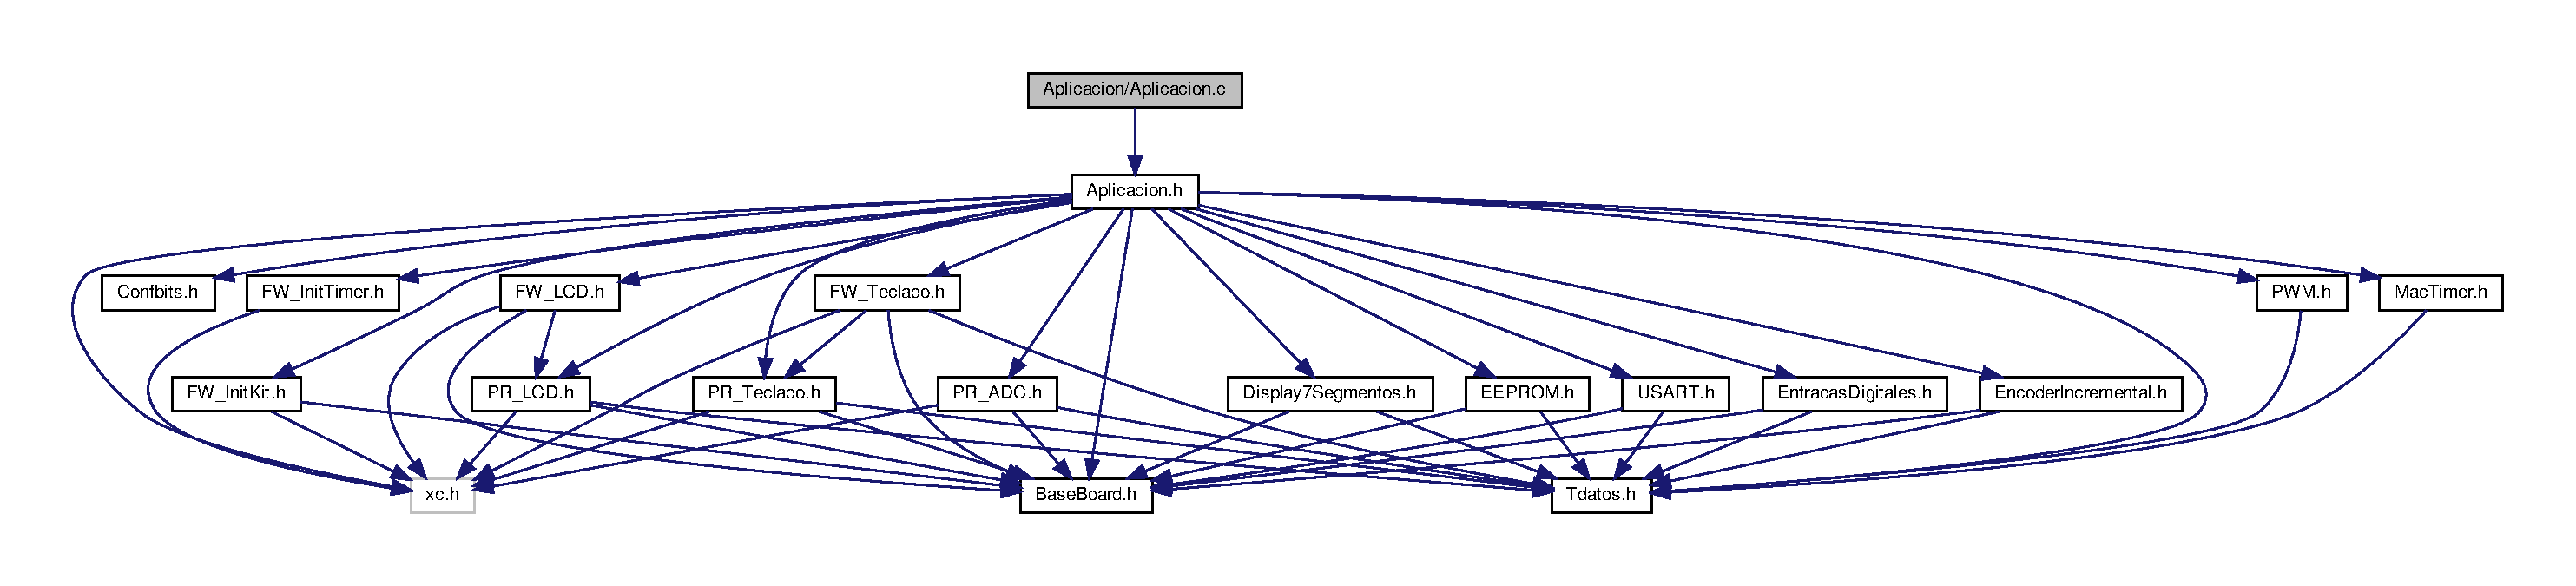
\includegraphics[width=350pt]{db/d10/Aplicacion_8c__incl}
\end{center}
\end{figure}
\subsection*{Funciones}
\begin{DoxyCompactItemize}
\item 
void \hyperlink{Aplicacion_8c_a1c8d673b24659a71245bca4363fa1887}{Aplicacion} (void)
\begin{DoxyCompactList}\small\item\em Funcion principal. \end{DoxyCompactList}\end{DoxyCompactItemize}


\subsection{Documentación de las funciones}
\mbox{\Hypertarget{Aplicacion_8c_a1c8d673b24659a71245bca4363fa1887}\label{Aplicacion_8c_a1c8d673b24659a71245bca4363fa1887}} 
\index{Aplicacion.\+c@{Aplicacion.\+c}!Aplicacion@{Aplicacion}}
\index{Aplicacion@{Aplicacion}!Aplicacion.\+c@{Aplicacion.\+c}}
\subsubsection{\texorpdfstring{Aplicacion()}{Aplicacion()}}
{\footnotesize\ttfamily void Aplicacion (\begin{DoxyParamCaption}\item[{void}]{ }\end{DoxyParamCaption})}



Funcion principal. 

\begin{DoxyAuthor}{Autor}
Nicolas Ferragamo \href{mailto:nferragamo@est.frba.utn.edu.ar}{\tt nferragamo@est.\+frba.\+utn.\+edu.\+ar} 
\end{DoxyAuthor}
\begin{DoxyDate}{Fecha}
13 de junio del 2019 
\end{DoxyDate}


Definición en la línea 84 del archivo Aplicacion.\+c.

Gráfico de llamadas a esta función\+:\nopagebreak
\begin{figure}[H]
\begin{center}
\leavevmode
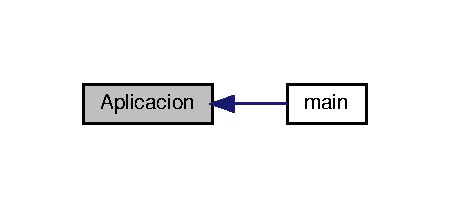
\includegraphics[width=216pt]{d8/db4/Aplicacion_8c_a1c8d673b24659a71245bca4363fa1887_icgraph}
\end{center}
\end{figure}

\hypertarget{FW__Display7Segmentos_8c}{}\section{Referencia del Archivo Firmware\+\_\+\+Driver/\+F\+W\+\_\+\+Display7\+Segmentos.c}
\label{FW__Display7Segmentos_8c}\index{Firmware\+\_\+\+Driver/\+F\+W\+\_\+\+Display7\+Segmentos.\+c@{Firmware\+\_\+\+Driver/\+F\+W\+\_\+\+Display7\+Segmentos.\+c}}
{\ttfamily \#include \char`\"{}xc.\+h\char`\"{}}\newline
{\ttfamily \#include \char`\"{}Display7\+Segmentos.\+h\char`\"{}}\newline
Dependencia gráfica adjunta para F\+W\+\_\+\+Display7\+Segmentos.\+c\+:\nopagebreak
\begin{figure}[H]
\begin{center}
\leavevmode
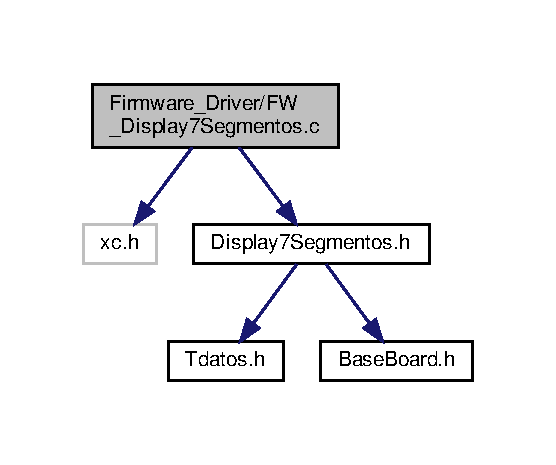
\includegraphics[width=267pt]{dc/dad/FW__Display7Segmentos_8c__incl}
\end{center}
\end{figure}
\subsection*{defines}
\begin{DoxyCompactItemize}
\item 
\#define \hyperlink{FW__Display7Segmentos_8c_a8cb7198d8e8f9b83a161b6d8f15e55cc}{D\+I\+G\+I\+T\+O0}~0
\item 
\#define \hyperlink{FW__Display7Segmentos_8c_a2e11b699b5e17408ee0fd7ce228e218e}{D\+I\+G\+I\+T\+O1}~1
\item 
\#define \hyperlink{FW__Display7Segmentos_8c_abced69cbedd0f7702a5af3d195c816b4}{D\+I\+G\+I\+T\+O2}~2
\item 
\#define \hyperlink{FW__Display7Segmentos_8c_a15fb113f69d249da1871b59d6c3257ec}{D\+I\+G\+I\+T\+O3}~3
\end{DoxyCompactItemize}
\subsection*{Funciones}
\begin{DoxyCompactItemize}
\item 
void \hyperlink{FW__Display7Segmentos_8c_a41b93045d294c7b52da4d1aa857383dd}{D\+P\+\_\+\+Barrido\+Display} (void)
\begin{DoxyCompactList}\small\item\em Realiza el barrido de los displays. \end{DoxyCompactList}\item 
void \hyperlink{FW__Display7Segmentos_8c_a372f00db9001b490f7cec5e8d86b559b}{D\+P\+\_\+\+Tic} (void)
\begin{DoxyCompactList}\small\item\em Se encarga de la demora del barrido. \end{DoxyCompactList}\end{DoxyCompactItemize}
\subsection*{Variables}
\begin{DoxyCompactItemize}
\item 
volatile \hyperlink{Tdatos_8h_aba7bc1797add20fe3efdf37ced1182c5}{uint8\+\_\+t} \hyperlink{FW__Display7Segmentos_8c_a65e480a33e370b81cef253cb71d2a22b}{D\+P\+\_\+\+Delay} = \hyperlink{Display7Segmentos_8h_a664b6ba4767ee385ae6010587d9d8b9a}{D\+P\+\_\+\+T\+IC}
\end{DoxyCompactItemize}


\subsection{Documentación de los \textquotesingle{}defines\textquotesingle{}}
\mbox{\Hypertarget{FW__Display7Segmentos_8c_a8cb7198d8e8f9b83a161b6d8f15e55cc}\label{FW__Display7Segmentos_8c_a8cb7198d8e8f9b83a161b6d8f15e55cc}} 
\index{F\+W\+\_\+\+Display7\+Segmentos.\+c@{F\+W\+\_\+\+Display7\+Segmentos.\+c}!D\+I\+G\+I\+T\+O0@{D\+I\+G\+I\+T\+O0}}
\index{D\+I\+G\+I\+T\+O0@{D\+I\+G\+I\+T\+O0}!F\+W\+\_\+\+Display7\+Segmentos.\+c@{F\+W\+\_\+\+Display7\+Segmentos.\+c}}
\subsubsection{\texorpdfstring{D\+I\+G\+I\+T\+O0}{DIGITO0}}
{\footnotesize\ttfamily \#define D\+I\+G\+I\+T\+O0~0}



Definición en la línea 45 del archivo F\+W\+\_\+\+Display7\+Segmentos.\+c.

\mbox{\Hypertarget{FW__Display7Segmentos_8c_a2e11b699b5e17408ee0fd7ce228e218e}\label{FW__Display7Segmentos_8c_a2e11b699b5e17408ee0fd7ce228e218e}} 
\index{F\+W\+\_\+\+Display7\+Segmentos.\+c@{F\+W\+\_\+\+Display7\+Segmentos.\+c}!D\+I\+G\+I\+T\+O1@{D\+I\+G\+I\+T\+O1}}
\index{D\+I\+G\+I\+T\+O1@{D\+I\+G\+I\+T\+O1}!F\+W\+\_\+\+Display7\+Segmentos.\+c@{F\+W\+\_\+\+Display7\+Segmentos.\+c}}
\subsubsection{\texorpdfstring{D\+I\+G\+I\+T\+O1}{DIGITO1}}
{\footnotesize\ttfamily \#define D\+I\+G\+I\+T\+O1~1}



Definición en la línea 46 del archivo F\+W\+\_\+\+Display7\+Segmentos.\+c.

\mbox{\Hypertarget{FW__Display7Segmentos_8c_abced69cbedd0f7702a5af3d195c816b4}\label{FW__Display7Segmentos_8c_abced69cbedd0f7702a5af3d195c816b4}} 
\index{F\+W\+\_\+\+Display7\+Segmentos.\+c@{F\+W\+\_\+\+Display7\+Segmentos.\+c}!D\+I\+G\+I\+T\+O2@{D\+I\+G\+I\+T\+O2}}
\index{D\+I\+G\+I\+T\+O2@{D\+I\+G\+I\+T\+O2}!F\+W\+\_\+\+Display7\+Segmentos.\+c@{F\+W\+\_\+\+Display7\+Segmentos.\+c}}
\subsubsection{\texorpdfstring{D\+I\+G\+I\+T\+O2}{DIGITO2}}
{\footnotesize\ttfamily \#define D\+I\+G\+I\+T\+O2~2}



Definición en la línea 47 del archivo F\+W\+\_\+\+Display7\+Segmentos.\+c.

\mbox{\Hypertarget{FW__Display7Segmentos_8c_a15fb113f69d249da1871b59d6c3257ec}\label{FW__Display7Segmentos_8c_a15fb113f69d249da1871b59d6c3257ec}} 
\index{F\+W\+\_\+\+Display7\+Segmentos.\+c@{F\+W\+\_\+\+Display7\+Segmentos.\+c}!D\+I\+G\+I\+T\+O3@{D\+I\+G\+I\+T\+O3}}
\index{D\+I\+G\+I\+T\+O3@{D\+I\+G\+I\+T\+O3}!F\+W\+\_\+\+Display7\+Segmentos.\+c@{F\+W\+\_\+\+Display7\+Segmentos.\+c}}
\subsubsection{\texorpdfstring{D\+I\+G\+I\+T\+O3}{DIGITO3}}
{\footnotesize\ttfamily \#define D\+I\+G\+I\+T\+O3~3}



Definición en la línea 48 del archivo F\+W\+\_\+\+Display7\+Segmentos.\+c.



\subsection{Documentación de las funciones}
\mbox{\Hypertarget{FW__Display7Segmentos_8c_a41b93045d294c7b52da4d1aa857383dd}\label{FW__Display7Segmentos_8c_a41b93045d294c7b52da4d1aa857383dd}} 
\index{F\+W\+\_\+\+Display7\+Segmentos.\+c@{F\+W\+\_\+\+Display7\+Segmentos.\+c}!D\+P\+\_\+\+Barrido\+Display@{D\+P\+\_\+\+Barrido\+Display}}
\index{D\+P\+\_\+\+Barrido\+Display@{D\+P\+\_\+\+Barrido\+Display}!F\+W\+\_\+\+Display7\+Segmentos.\+c@{F\+W\+\_\+\+Display7\+Segmentos.\+c}}
\subsubsection{\texorpdfstring{D\+P\+\_\+\+Barrido\+Display()}{DP\_BarridoDisplay()}}
{\footnotesize\ttfamily void D\+P\+\_\+\+Barrido\+Display (\begin{DoxyParamCaption}\item[{void}]{ }\end{DoxyParamCaption})}



Realiza el barrido de los displays. 

\begin{DoxyAuthor}{Autor}
Nicol�s Exequiel Ferragamo 
\end{DoxyAuthor}
\begin{DoxyDate}{Fecha}
30 de septiembre de 2019 
\end{DoxyDate}

\begin{DoxyParams}[1]{Parámetros}
\mbox{\tt in}  & {\em void} & \\
\hline
\mbox{\tt out}  & {\em void} & \\
\hline
\end{DoxyParams}


Definición en la línea 89 del archivo F\+W\+\_\+\+Display7\+Segmentos.\+c.

\mbox{\Hypertarget{FW__Display7Segmentos_8c_a372f00db9001b490f7cec5e8d86b559b}\label{FW__Display7Segmentos_8c_a372f00db9001b490f7cec5e8d86b559b}} 
\index{F\+W\+\_\+\+Display7\+Segmentos.\+c@{F\+W\+\_\+\+Display7\+Segmentos.\+c}!D\+P\+\_\+\+Tic@{D\+P\+\_\+\+Tic}}
\index{D\+P\+\_\+\+Tic@{D\+P\+\_\+\+Tic}!F\+W\+\_\+\+Display7\+Segmentos.\+c@{F\+W\+\_\+\+Display7\+Segmentos.\+c}}
\subsubsection{\texorpdfstring{D\+P\+\_\+\+Tic()}{DP\_Tic()}}
{\footnotesize\ttfamily void D\+P\+\_\+\+Tic (\begin{DoxyParamCaption}\item[{void}]{ }\end{DoxyParamCaption})}



Se encarga de la demora del barrido. 

\begin{DoxyAuthor}{Autor}
Nicol�s Exequiel Ferragamo 
\end{DoxyAuthor}
\begin{DoxyDate}{Fecha}
30 de septiembre de 2019 
\end{DoxyDate}

\begin{DoxyParams}[1]{Parámetros}
\mbox{\tt in}  & {\em void} & \\
\hline
\mbox{\tt out}  & {\em void} & \\
\hline
\end{DoxyParams}


Definición en la línea 136 del archivo F\+W\+\_\+\+Display7\+Segmentos.\+c.



\subsection{Documentación de las variables}
\mbox{\Hypertarget{FW__Display7Segmentos_8c_a65e480a33e370b81cef253cb71d2a22b}\label{FW__Display7Segmentos_8c_a65e480a33e370b81cef253cb71d2a22b}} 
\index{F\+W\+\_\+\+Display7\+Segmentos.\+c@{F\+W\+\_\+\+Display7\+Segmentos.\+c}!D\+P\+\_\+\+Delay@{D\+P\+\_\+\+Delay}}
\index{D\+P\+\_\+\+Delay@{D\+P\+\_\+\+Delay}!F\+W\+\_\+\+Display7\+Segmentos.\+c@{F\+W\+\_\+\+Display7\+Segmentos.\+c}}
\subsubsection{\texorpdfstring{D\+P\+\_\+\+Delay}{DP\_Delay}}
{\footnotesize\ttfamily volatile \hyperlink{Tdatos_8h_aba7bc1797add20fe3efdf37ced1182c5}{uint8\+\_\+t} D\+P\+\_\+\+Delay = \hyperlink{Display7Segmentos_8h_a664b6ba4767ee385ae6010587d9d8b9a}{D\+P\+\_\+\+T\+IC}}



Definición en la línea 64 del archivo F\+W\+\_\+\+Display7\+Segmentos.\+c.


\hypertarget{FW__EncoderIncremental_8c}{}\section{Referencia del Archivo Firmware\+\_\+\+Driver/\+F\+W\+\_\+\+Encoder\+Incremental.c}
\label{FW__EncoderIncremental_8c}\index{Firmware\+\_\+\+Driver/\+F\+W\+\_\+\+Encoder\+Incremental.\+c@{Firmware\+\_\+\+Driver/\+F\+W\+\_\+\+Encoder\+Incremental.\+c}}
{\ttfamily \#include $<$xc.\+h$>$}\newline
{\ttfamily \#include \char`\"{}Tdatos.\+h\char`\"{}}\newline
{\ttfamily \#include \char`\"{}Base\+Board.\+h\char`\"{}}\newline
{\ttfamily \#include \char`\"{}Encoder\+Incremental.\+h\char`\"{}}\newline
{\ttfamily \#include \char`\"{}Display7\+Segmentos.\+h\char`\"{}}\newline
Dependencia gráfica adjunta para F\+W\+\_\+\+Encoder\+Incremental.\+c\+:\nopagebreak
\begin{figure}[H]
\begin{center}
\leavevmode
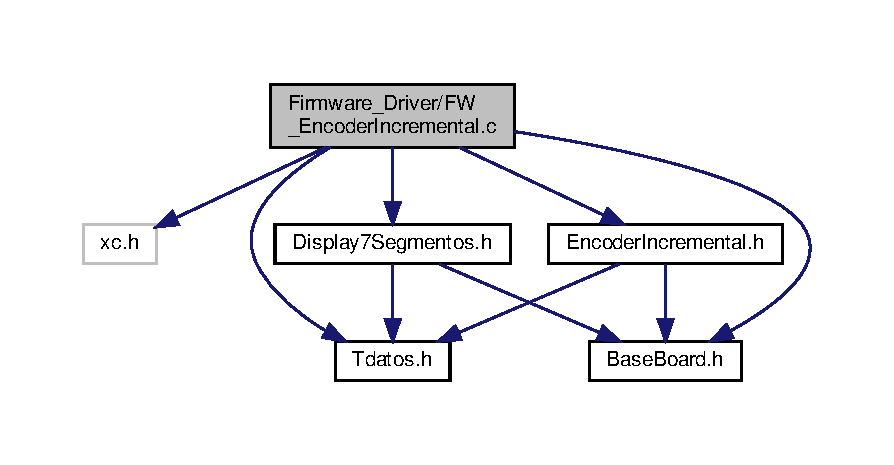
\includegraphics[width=350pt]{d4/d10/FW__EncoderIncremental_8c__incl}
\end{center}
\end{figure}
\subsection*{Funciones}
\begin{DoxyCompactItemize}
\item 
void \hyperlink{FW__EncoderIncremental_8c_a90a4d0e96e4a9aac93bb2b59e2f1b624}{E\+D\+E\+R\+\_\+\+Interrupt} (void)
\item 
void \hyperlink{FW__EncoderIncremental_8c_a11701efeb48e9b7b95efe7a958a91401}{E\+D\+E\+R\+\_\+\+Tic} (void)
\begin{DoxyCompactList}\small\item\em Se encarga de la demora. \end{DoxyCompactList}\end{DoxyCompactItemize}
\subsection*{Variables}
\begin{DoxyCompactItemize}
\item 
volatile \hyperlink{Tdatos_8h_aba7bc1797add20fe3efdf37ced1182c5}{uint8\+\_\+t} \hyperlink{FW__EncoderIncremental_8c_a7a16d365adb64dd67685e78369350faf}{E\+D\+E\+R\+\_\+\+Delay} = \hyperlink{EncoderIncremental_8h_a54aee7bed904715e92c3c6e9f1801f03}{E\+D\+E\+R\+\_\+\+D\+E\+L\+AY}
\item 
volatile \hyperlink{Tdatos_8h_aba7bc1797add20fe3efdf37ced1182c5}{uint8\+\_\+t} \hyperlink{FW__EncoderIncremental_8c_acec90ea3b9fe87fc336faf998a18f74a}{E\+D\+E\+R\+\_\+\+Flag\+Canal} = 0
\end{DoxyCompactItemize}


\subsection{Documentación de las funciones}
\mbox{\Hypertarget{FW__EncoderIncremental_8c_a90a4d0e96e4a9aac93bb2b59e2f1b624}\label{FW__EncoderIncremental_8c_a90a4d0e96e4a9aac93bb2b59e2f1b624}} 
\index{F\+W\+\_\+\+Encoder\+Incremental.\+c@{F\+W\+\_\+\+Encoder\+Incremental.\+c}!E\+D\+E\+R\+\_\+\+Interrupt@{E\+D\+E\+R\+\_\+\+Interrupt}}
\index{E\+D\+E\+R\+\_\+\+Interrupt@{E\+D\+E\+R\+\_\+\+Interrupt}!F\+W\+\_\+\+Encoder\+Incremental.\+c@{F\+W\+\_\+\+Encoder\+Incremental.\+c}}
\subsubsection{\texorpdfstring{E\+D\+E\+R\+\_\+\+Interrupt()}{EDER\_Interrupt()}}
{\footnotesize\ttfamily void E\+D\+E\+R\+\_\+\+Interrupt (\begin{DoxyParamCaption}\item[{void}]{ }\end{DoxyParamCaption})}



Definición en la línea 113 del archivo F\+W\+\_\+\+Encoder\+Incremental.\+c.

\mbox{\Hypertarget{FW__EncoderIncremental_8c_a11701efeb48e9b7b95efe7a958a91401}\label{FW__EncoderIncremental_8c_a11701efeb48e9b7b95efe7a958a91401}} 
\index{F\+W\+\_\+\+Encoder\+Incremental.\+c@{F\+W\+\_\+\+Encoder\+Incremental.\+c}!E\+D\+E\+R\+\_\+\+Tic@{E\+D\+E\+R\+\_\+\+Tic}}
\index{E\+D\+E\+R\+\_\+\+Tic@{E\+D\+E\+R\+\_\+\+Tic}!F\+W\+\_\+\+Encoder\+Incremental.\+c@{F\+W\+\_\+\+Encoder\+Incremental.\+c}}
\subsubsection{\texorpdfstring{E\+D\+E\+R\+\_\+\+Tic()}{EDER\_Tic()}}
{\footnotesize\ttfamily void E\+D\+E\+R\+\_\+\+Tic (\begin{DoxyParamCaption}\item[{void}]{ }\end{DoxyParamCaption})}



Se encarga de la demora. 

\begin{DoxyAuthor}{Autor}

\end{DoxyAuthor}
\begin{DoxyDate}{Fecha}

\end{DoxyDate}

\begin{DoxyParams}[1]{Parámetros}
\mbox{\tt in}  & {\em void} & \\
\hline
\mbox{\tt out}  & {\em void} & \\
\hline
\end{DoxyParams}


Definición en la línea 145 del archivo F\+W\+\_\+\+Encoder\+Incremental.\+c.



\subsection{Documentación de las variables}
\mbox{\Hypertarget{FW__EncoderIncremental_8c_a7a16d365adb64dd67685e78369350faf}\label{FW__EncoderIncremental_8c_a7a16d365adb64dd67685e78369350faf}} 
\index{F\+W\+\_\+\+Encoder\+Incremental.\+c@{F\+W\+\_\+\+Encoder\+Incremental.\+c}!E\+D\+E\+R\+\_\+\+Delay@{E\+D\+E\+R\+\_\+\+Delay}}
\index{E\+D\+E\+R\+\_\+\+Delay@{E\+D\+E\+R\+\_\+\+Delay}!F\+W\+\_\+\+Encoder\+Incremental.\+c@{F\+W\+\_\+\+Encoder\+Incremental.\+c}}
\subsubsection{\texorpdfstring{E\+D\+E\+R\+\_\+\+Delay}{EDER\_Delay}}
{\footnotesize\ttfamily volatile \hyperlink{Tdatos_8h_aba7bc1797add20fe3efdf37ced1182c5}{uint8\+\_\+t} E\+D\+E\+R\+\_\+\+Delay = \hyperlink{EncoderIncremental_8h_a54aee7bed904715e92c3c6e9f1801f03}{E\+D\+E\+R\+\_\+\+D\+E\+L\+AY}}



Definición en la línea 67 del archivo F\+W\+\_\+\+Encoder\+Incremental.\+c.

\mbox{\Hypertarget{FW__EncoderIncremental_8c_acec90ea3b9fe87fc336faf998a18f74a}\label{FW__EncoderIncremental_8c_acec90ea3b9fe87fc336faf998a18f74a}} 
\index{F\+W\+\_\+\+Encoder\+Incremental.\+c@{F\+W\+\_\+\+Encoder\+Incremental.\+c}!E\+D\+E\+R\+\_\+\+Flag\+Canal@{E\+D\+E\+R\+\_\+\+Flag\+Canal}}
\index{E\+D\+E\+R\+\_\+\+Flag\+Canal@{E\+D\+E\+R\+\_\+\+Flag\+Canal}!F\+W\+\_\+\+Encoder\+Incremental.\+c@{F\+W\+\_\+\+Encoder\+Incremental.\+c}}
\subsubsection{\texorpdfstring{E\+D\+E\+R\+\_\+\+Flag\+Canal}{EDER\_FlagCanal}}
{\footnotesize\ttfamily volatile \hyperlink{Tdatos_8h_aba7bc1797add20fe3efdf37ced1182c5}{uint8\+\_\+t} E\+D\+E\+R\+\_\+\+Flag\+Canal = 0}



Definición en la línea 68 del archivo F\+W\+\_\+\+Encoder\+Incremental.\+c.


\hypertarget{FW__EntradasDigitales_8c}{}\section{Referencia del Archivo Firmware\+\_\+\+Driver/\+F\+W\+\_\+\+Entradas\+Digitales.c}
\label{FW__EntradasDigitales_8c}\index{Firmware\+\_\+\+Driver/\+F\+W\+\_\+\+Entradas\+Digitales.\+c@{Firmware\+\_\+\+Driver/\+F\+W\+\_\+\+Entradas\+Digitales.\+c}}
{\ttfamily \#include $<$xc.\+h$>$}\newline
{\ttfamily \#include \char`\"{}Tdatos.\+h\char`\"{}}\newline
{\ttfamily \#include \char`\"{}Base\+Board.\+h\char`\"{}}\newline
{\ttfamily \#include \char`\"{}Entradas\+Digitales.\+h\char`\"{}}\newline
Dependencia gráfica adjunta para F\+W\+\_\+\+Entradas\+Digitales.\+c\+:\nopagebreak
\begin{figure}[H]
\begin{center}
\leavevmode
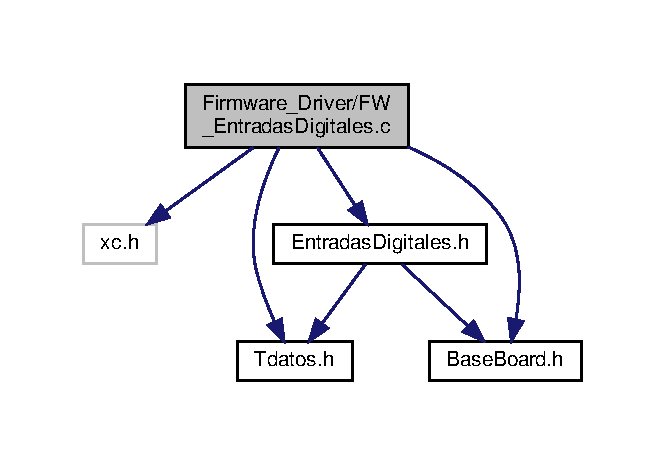
\includegraphics[width=319pt]{dd/d59/FW__EntradasDigitales_8c__incl}
\end{center}
\end{figure}
\subsection*{Funciones}
\begin{DoxyCompactItemize}
\item 
void \hyperlink{FW__EntradasDigitales_8c_aae3299a4d1a16965cb68fdb0dfe20a2a}{E\+D\+\_\+\+Debounce} (void)
\begin{DoxyCompactList}\small\item\em Funcion para el debounce de las entradas digitales. \end{DoxyCompactList}\item 
void \hyperlink{FW__EntradasDigitales_8c_a37cb4f85d5ecd1e06ebee2aff2cea677}{E\+D\+\_\+\+Tic} (void)
\begin{DoxyCompactList}\small\item\em Funcion para el debounce de las entradas digitales. \end{DoxyCompactList}\end{DoxyCompactItemize}
\subsection*{Variables}
\begin{DoxyCompactItemize}
\item 
volatile \hyperlink{Tdatos_8h_aba7bc1797add20fe3efdf37ced1182c5}{uint8\+\_\+t} \hyperlink{FW__EntradasDigitales_8c_a85bf28760a0b8f0d354faa8e0560a4f8}{E\+D\+\_\+\+Delay} = \hyperlink{EntradasDigitales_8h_a63fb786778d627ac652386fea3980b26}{E\+D\+\_\+\+T\+IC}
\end{DoxyCompactItemize}


\subsection{Documentación de las funciones}
\mbox{\Hypertarget{FW__EntradasDigitales_8c_aae3299a4d1a16965cb68fdb0dfe20a2a}\label{FW__EntradasDigitales_8c_aae3299a4d1a16965cb68fdb0dfe20a2a}} 
\index{F\+W\+\_\+\+Entradas\+Digitales.\+c@{F\+W\+\_\+\+Entradas\+Digitales.\+c}!E\+D\+\_\+\+Debounce@{E\+D\+\_\+\+Debounce}}
\index{E\+D\+\_\+\+Debounce@{E\+D\+\_\+\+Debounce}!F\+W\+\_\+\+Entradas\+Digitales.\+c@{F\+W\+\_\+\+Entradas\+Digitales.\+c}}
\subsubsection{\texorpdfstring{E\+D\+\_\+\+Debounce()}{ED\_Debounce()}}
{\footnotesize\ttfamily void E\+D\+\_\+\+Debounce (\begin{DoxyParamCaption}\item[{void}]{ }\end{DoxyParamCaption})}



Funcion para el debounce de las entradas digitales. 

\begin{DoxyAuthor}{Autor}
Nicolas Ferragamo 
\end{DoxyAuthor}
\begin{DoxyDate}{Fecha}
30 de septiembre de 2019 
\end{DoxyDate}

\begin{DoxyParams}[1]{Parámetros}
\mbox{\tt in}  & {\em void} & \\
\hline
\mbox{\tt out}  & {\em void} & \\
\hline
\end{DoxyParams}
\begin{DoxyReturn}{Devuelve}
void 
\end{DoxyReturn}


Definición en la línea 94 del archivo F\+W\+\_\+\+Entradas\+Digitales.\+c.

\mbox{\Hypertarget{FW__EntradasDigitales_8c_a37cb4f85d5ecd1e06ebee2aff2cea677}\label{FW__EntradasDigitales_8c_a37cb4f85d5ecd1e06ebee2aff2cea677}} 
\index{F\+W\+\_\+\+Entradas\+Digitales.\+c@{F\+W\+\_\+\+Entradas\+Digitales.\+c}!E\+D\+\_\+\+Tic@{E\+D\+\_\+\+Tic}}
\index{E\+D\+\_\+\+Tic@{E\+D\+\_\+\+Tic}!F\+W\+\_\+\+Entradas\+Digitales.\+c@{F\+W\+\_\+\+Entradas\+Digitales.\+c}}
\subsubsection{\texorpdfstring{E\+D\+\_\+\+Tic()}{ED\_Tic()}}
{\footnotesize\ttfamily void E\+D\+\_\+\+Tic (\begin{DoxyParamCaption}\item[{void}]{ }\end{DoxyParamCaption})}



Funcion para el debounce de las entradas digitales. 

\begin{DoxyAuthor}{Autor}
Nicolas Ferragamo 
\end{DoxyAuthor}
\begin{DoxyDate}{Fecha}
30 de septiembre de 2019 
\end{DoxyDate}

\begin{DoxyParams}[1]{Parámetros}
\mbox{\tt in}  & {\em void} & \\
\hline
\mbox{\tt out}  & {\em void} & \\
\hline
\end{DoxyParams}
\begin{DoxyReturn}{Devuelve}
void 
\end{DoxyReturn}


Definición en la línea 151 del archivo F\+W\+\_\+\+Entradas\+Digitales.\+c.



\subsection{Documentación de las variables}
\mbox{\Hypertarget{FW__EntradasDigitales_8c_a85bf28760a0b8f0d354faa8e0560a4f8}\label{FW__EntradasDigitales_8c_a85bf28760a0b8f0d354faa8e0560a4f8}} 
\index{F\+W\+\_\+\+Entradas\+Digitales.\+c@{F\+W\+\_\+\+Entradas\+Digitales.\+c}!E\+D\+\_\+\+Delay@{E\+D\+\_\+\+Delay}}
\index{E\+D\+\_\+\+Delay@{E\+D\+\_\+\+Delay}!F\+W\+\_\+\+Entradas\+Digitales.\+c@{F\+W\+\_\+\+Entradas\+Digitales.\+c}}
\subsubsection{\texorpdfstring{E\+D\+\_\+\+Delay}{ED\_Delay}}
{\footnotesize\ttfamily volatile \hyperlink{Tdatos_8h_aba7bc1797add20fe3efdf37ced1182c5}{uint8\+\_\+t} E\+D\+\_\+\+Delay = \hyperlink{EntradasDigitales_8h_a63fb786778d627ac652386fea3980b26}{E\+D\+\_\+\+T\+IC}}



Definición en la línea 66 del archivo F\+W\+\_\+\+Entradas\+Digitales.\+c.


\hypertarget{FW__Interrupt_8c}{}\section{Referencia del Archivo Firmware\+\_\+\+Driver/\+F\+W\+\_\+\+Interrupt.c}
\label{FW__Interrupt_8c}\index{Firmware\+\_\+\+Driver/\+F\+W\+\_\+\+Interrupt.\+c@{Firmware\+\_\+\+Driver/\+F\+W\+\_\+\+Interrupt.\+c}}
{\ttfamily \#include $<$xc.\+h$>$}\newline
{\ttfamily \#include \char`\"{}Tdatos.\+h\char`\"{}}\newline
{\ttfamily \#include \char`\"{}Entradas\+Digitales.\+h\char`\"{}}\newline
{\ttfamily \#include \char`\"{}Display7\+Segmentos.\+h\char`\"{}}\newline
{\ttfamily \#include \char`\"{}P\+R\+\_\+\+Teclado.\+h\char`\"{}}\newline
{\ttfamily \#include \char`\"{}Encoder\+Incremental.\+h\char`\"{}}\newline
{\ttfamily \#include \char`\"{}Mac\+Timer.\+h\char`\"{}}\newline
Dependencia gráfica adjunta para F\+W\+\_\+\+Interrupt.\+c\+:\nopagebreak
\begin{figure}[H]
\begin{center}
\leavevmode
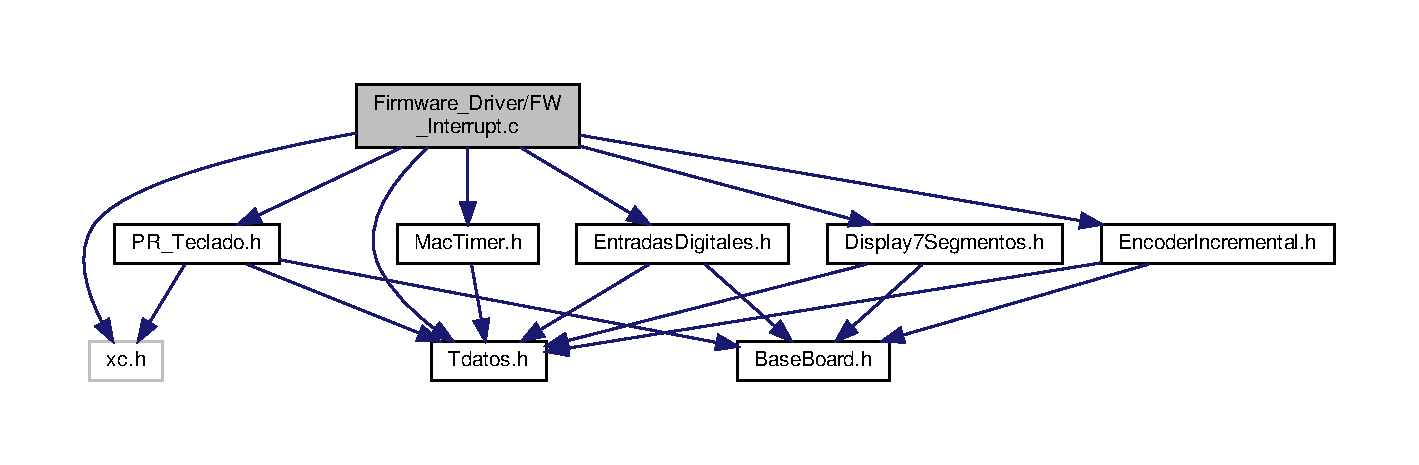
\includegraphics[width=350pt]{d1/d2f/FW__Interrupt_8c__incl}
\end{center}
\end{figure}
\subsection*{Funciones}
\begin{DoxyCompactItemize}
\item 
void \hyperlink{FW__Interrupt_8c_a9c2f60604071e2b4583e463e6825e708}{\+\_\+\+\_\+interrupt} ()
\begin{DoxyCompactList}\small\item\em Funcion de interrupcion. \end{DoxyCompactList}\end{DoxyCompactItemize}


\subsection{Documentación de las funciones}
\mbox{\Hypertarget{FW__Interrupt_8c_a9c2f60604071e2b4583e463e6825e708}\label{FW__Interrupt_8c_a9c2f60604071e2b4583e463e6825e708}} 
\index{F\+W\+\_\+\+Interrupt.\+c@{F\+W\+\_\+\+Interrupt.\+c}!\+\_\+\+\_\+interrupt@{\+\_\+\+\_\+interrupt}}
\index{\+\_\+\+\_\+interrupt@{\+\_\+\+\_\+interrupt}!F\+W\+\_\+\+Interrupt.\+c@{F\+W\+\_\+\+Interrupt.\+c}}
\subsubsection{\texorpdfstring{\+\_\+\+\_\+interrupt()}{\_\_interrupt()}}
{\footnotesize\ttfamily \+\_\+\+\_\+interrupt (\begin{DoxyParamCaption}{ }\end{DoxyParamCaption})}



Funcion de interrupcion. 

\begin{DoxyAuthor}{Autor}
Nicolas Ferragamo 
\end{DoxyAuthor}
\begin{DoxyDate}{Fecha}
23 de abril de 2019 
\end{DoxyDate}

\begin{DoxyParams}[1]{Parámetros}
\mbox{\tt in}  & {\em void} & \\
\hline
\mbox{\tt out}  & {\em void} & \\
\hline
\end{DoxyParams}
\begin{DoxyReturn}{Devuelve}
void 
\end{DoxyReturn}


Definición en la línea 66 del archivo F\+W\+\_\+\+Interrupt.\+c.


\hypertarget{FW__LCD_8c}{}\section{Referencia del Archivo Firmware\+\_\+\+Driver/\+F\+W\+\_\+\+L\+CD.c}
\label{FW__LCD_8c}\index{Firmware\+\_\+\+Driver/\+F\+W\+\_\+\+L\+C\+D.\+c@{Firmware\+\_\+\+Driver/\+F\+W\+\_\+\+L\+C\+D.\+c}}
{\ttfamily \#include \char`\"{}F\+W\+\_\+\+L\+C\+D.\+h\char`\"{}}\newline
Dependencia gráfica adjunta para F\+W\+\_\+\+L\+C\+D.\+c\+:\nopagebreak
\begin{figure}[H]
\begin{center}
\leavevmode
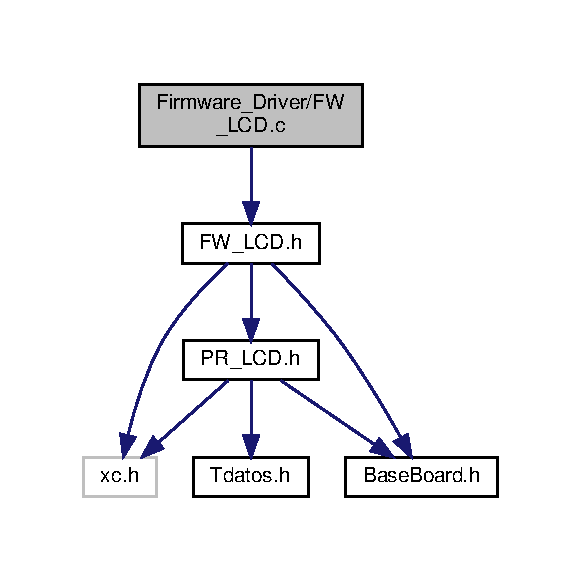
\includegraphics[width=279pt]{dd/d3e/FW__LCD_8c__incl}
\end{center}
\end{figure}
\subsection*{defines}
\begin{DoxyCompactItemize}
\item 
\#define \hyperlink{FW__LCD_8c_a27fc19637a3e83d6a1836349f57beeea}{L\+C\+D\+\_\+\+E\+N\+T\+R\+A\+DA}~0x\+F0
\begin{DoxyCompactList}\small\item\em Esto es para invertir el bus de datos y poder. \end{DoxyCompactList}\item 
\#define \hyperlink{FW__LCD_8c_a372d8466c4b1b318bca88c3d5a454262}{L\+C\+D\+\_\+\+S\+A\+L\+I\+DA}~0x0F
\begin{DoxyCompactList}\small\item\em leer cuando necesito ver si est� busy.. \end{DoxyCompactList}\item 
\#define \hyperlink{FW__LCD_8c_ac8dd1658e235f174d1cabae5c438943d}{L\+C\+D\+\_\+\+B\+U\+SY}~P\+O\+R\+T\+Dbits.\+R\+D7
\begin{DoxyCompactList}\small\item\em Con estos defines me abstraigo del hardware. \end{DoxyCompactList}\item 
\#define \hyperlink{FW__LCD_8c_ae7fe5d669c432901d21fef38c9743dfe}{L\+C\+D\+\_\+\+B\+U\+S\+\_\+\+D\+IR}~T\+R\+I\+SD
\item 
\#define \hyperlink{FW__LCD_8c_aac80e54c3d1d3592462eb30e6cac6ca6}{L\+C\+D\+\_\+\+T\+R\+UE}~0x1
\item 
\#define \hyperlink{FW__LCD_8c_a9719ec9752a485662fafc37d1d54f98e}{L\+C\+D\+\_\+\+F\+A\+L\+SE}~0x0
\end{DoxyCompactItemize}
\subsection*{Funciones}
\begin{DoxyCompactItemize}
\item 
void \hyperlink{FW__LCD_8c_a72115baa02a7c5fb1c015ac3cea2308d}{L\+C\+D\+\_\+\+Read\+Busy} (void)
\item 
void \hyperlink{FW__LCD_8c_a8dbf68ce3dbf3821499c9b5106838700}{L\+C\+D\+\_\+\+Write\+C\+MD} (\hyperlink{Tdatos_8h_aba7bc1797add20fe3efdf37ced1182c5}{uint8\+\_\+t} comando)
\item 
void \hyperlink{FW__LCD_8c_aa0b64783f3a2f265b3bda0b9d92d7d89}{L\+C\+D\+\_\+\+Write} (\hyperlink{Tdatos_8h_aba7bc1797add20fe3efdf37ced1182c5}{uint8\+\_\+t} dato)
\begin{DoxyCompactList}\small\item\em Se encarga de escribir un dato en bus de a un nibble por vez. \end{DoxyCompactList}\item 
void \hyperlink{FW__LCD_8c_a5ced9cb01df0ef6d721dec73ae29b11b}{L\+C\+D\+\_\+\+Write\+Data} (\hyperlink{Tdatos_8h_aba7bc1797add20fe3efdf37ced1182c5}{uint8\+\_\+t} dato)
\item 
void \hyperlink{FW__LCD_8c_a9d705e44e019897df3cf52334f6d2083}{L\+C\+D\+\_\+\+Tic\+L\+CD} (void)
\begin{DoxyCompactList}\small\item\em Rutina necesaria para el fncionamiento del m�dulo. \end{DoxyCompactList}\end{DoxyCompactItemize}
\subsection*{Variables}
\begin{DoxyCompactItemize}
\item 
volatile \hyperlink{Tdatos_8h_aba7bc1797add20fe3efdf37ced1182c5}{uint8\+\_\+t} \hyperlink{FW__LCD_8c_a3dd55c3be6a5452edf6e1d8b8b90213f}{L\+C\+D\+\_\+\+Tout} = 0
\end{DoxyCompactItemize}


\subsection{Documentación de los \textquotesingle{}defines\textquotesingle{}}
\mbox{\Hypertarget{FW__LCD_8c_ae7fe5d669c432901d21fef38c9743dfe}\label{FW__LCD_8c_ae7fe5d669c432901d21fef38c9743dfe}} 
\index{F\+W\+\_\+\+L\+C\+D.\+c@{F\+W\+\_\+\+L\+C\+D.\+c}!L\+C\+D\+\_\+\+B\+U\+S\+\_\+\+D\+IR@{L\+C\+D\+\_\+\+B\+U\+S\+\_\+\+D\+IR}}
\index{L\+C\+D\+\_\+\+B\+U\+S\+\_\+\+D\+IR@{L\+C\+D\+\_\+\+B\+U\+S\+\_\+\+D\+IR}!F\+W\+\_\+\+L\+C\+D.\+c@{F\+W\+\_\+\+L\+C\+D.\+c}}
\subsubsection{\texorpdfstring{L\+C\+D\+\_\+\+B\+U\+S\+\_\+\+D\+IR}{LCD\_BUS\_DIR}}
{\footnotesize\ttfamily \#define L\+C\+D\+\_\+\+B\+U\+S\+\_\+\+D\+IR~T\+R\+I\+SD}



Definición en la línea 48 del archivo F\+W\+\_\+\+L\+C\+D.\+c.

\mbox{\Hypertarget{FW__LCD_8c_ac8dd1658e235f174d1cabae5c438943d}\label{FW__LCD_8c_ac8dd1658e235f174d1cabae5c438943d}} 
\index{F\+W\+\_\+\+L\+C\+D.\+c@{F\+W\+\_\+\+L\+C\+D.\+c}!L\+C\+D\+\_\+\+B\+U\+SY@{L\+C\+D\+\_\+\+B\+U\+SY}}
\index{L\+C\+D\+\_\+\+B\+U\+SY@{L\+C\+D\+\_\+\+B\+U\+SY}!F\+W\+\_\+\+L\+C\+D.\+c@{F\+W\+\_\+\+L\+C\+D.\+c}}
\subsubsection{\texorpdfstring{L\+C\+D\+\_\+\+B\+U\+SY}{LCD\_BUSY}}
{\footnotesize\ttfamily \#define L\+C\+D\+\_\+\+B\+U\+SY~P\+O\+R\+T\+Dbits.\+R\+D7}



Con estos defines me abstraigo del hardware. 



Definición en la línea 47 del archivo F\+W\+\_\+\+L\+C\+D.\+c.

\mbox{\Hypertarget{FW__LCD_8c_a27fc19637a3e83d6a1836349f57beeea}\label{FW__LCD_8c_a27fc19637a3e83d6a1836349f57beeea}} 
\index{F\+W\+\_\+\+L\+C\+D.\+c@{F\+W\+\_\+\+L\+C\+D.\+c}!L\+C\+D\+\_\+\+E\+N\+T\+R\+A\+DA@{L\+C\+D\+\_\+\+E\+N\+T\+R\+A\+DA}}
\index{L\+C\+D\+\_\+\+E\+N\+T\+R\+A\+DA@{L\+C\+D\+\_\+\+E\+N\+T\+R\+A\+DA}!F\+W\+\_\+\+L\+C\+D.\+c@{F\+W\+\_\+\+L\+C\+D.\+c}}
\subsubsection{\texorpdfstring{L\+C\+D\+\_\+\+E\+N\+T\+R\+A\+DA}{LCD\_ENTRADA}}
{\footnotesize\ttfamily \#define L\+C\+D\+\_\+\+E\+N\+T\+R\+A\+DA~0x\+F0}



Esto es para invertir el bus de datos y poder. 



Definición en la línea 45 del archivo F\+W\+\_\+\+L\+C\+D.\+c.

\mbox{\Hypertarget{FW__LCD_8c_a9719ec9752a485662fafc37d1d54f98e}\label{FW__LCD_8c_a9719ec9752a485662fafc37d1d54f98e}} 
\index{F\+W\+\_\+\+L\+C\+D.\+c@{F\+W\+\_\+\+L\+C\+D.\+c}!L\+C\+D\+\_\+\+F\+A\+L\+SE@{L\+C\+D\+\_\+\+F\+A\+L\+SE}}
\index{L\+C\+D\+\_\+\+F\+A\+L\+SE@{L\+C\+D\+\_\+\+F\+A\+L\+SE}!F\+W\+\_\+\+L\+C\+D.\+c@{F\+W\+\_\+\+L\+C\+D.\+c}}
\subsubsection{\texorpdfstring{L\+C\+D\+\_\+\+F\+A\+L\+SE}{LCD\_FALSE}}
{\footnotesize\ttfamily \#define L\+C\+D\+\_\+\+F\+A\+L\+SE~0x0}



Definición en la línea 51 del archivo F\+W\+\_\+\+L\+C\+D.\+c.

\mbox{\Hypertarget{FW__LCD_8c_a372d8466c4b1b318bca88c3d5a454262}\label{FW__LCD_8c_a372d8466c4b1b318bca88c3d5a454262}} 
\index{F\+W\+\_\+\+L\+C\+D.\+c@{F\+W\+\_\+\+L\+C\+D.\+c}!L\+C\+D\+\_\+\+S\+A\+L\+I\+DA@{L\+C\+D\+\_\+\+S\+A\+L\+I\+DA}}
\index{L\+C\+D\+\_\+\+S\+A\+L\+I\+DA@{L\+C\+D\+\_\+\+S\+A\+L\+I\+DA}!F\+W\+\_\+\+L\+C\+D.\+c@{F\+W\+\_\+\+L\+C\+D.\+c}}
\subsubsection{\texorpdfstring{L\+C\+D\+\_\+\+S\+A\+L\+I\+DA}{LCD\_SALIDA}}
{\footnotesize\ttfamily \#define L\+C\+D\+\_\+\+S\+A\+L\+I\+DA~0x0F}



leer cuando necesito ver si est� busy.. 



Definición en la línea 46 del archivo F\+W\+\_\+\+L\+C\+D.\+c.

\mbox{\Hypertarget{FW__LCD_8c_aac80e54c3d1d3592462eb30e6cac6ca6}\label{FW__LCD_8c_aac80e54c3d1d3592462eb30e6cac6ca6}} 
\index{F\+W\+\_\+\+L\+C\+D.\+c@{F\+W\+\_\+\+L\+C\+D.\+c}!L\+C\+D\+\_\+\+T\+R\+UE@{L\+C\+D\+\_\+\+T\+R\+UE}}
\index{L\+C\+D\+\_\+\+T\+R\+UE@{L\+C\+D\+\_\+\+T\+R\+UE}!F\+W\+\_\+\+L\+C\+D.\+c@{F\+W\+\_\+\+L\+C\+D.\+c}}
\subsubsection{\texorpdfstring{L\+C\+D\+\_\+\+T\+R\+UE}{LCD\_TRUE}}
{\footnotesize\ttfamily \#define L\+C\+D\+\_\+\+T\+R\+UE~0x1}



Definición en la línea 50 del archivo F\+W\+\_\+\+L\+C\+D.\+c.



\subsection{Documentación de las funciones}
\mbox{\Hypertarget{FW__LCD_8c_a72115baa02a7c5fb1c015ac3cea2308d}\label{FW__LCD_8c_a72115baa02a7c5fb1c015ac3cea2308d}} 
\index{F\+W\+\_\+\+L\+C\+D.\+c@{F\+W\+\_\+\+L\+C\+D.\+c}!L\+C\+D\+\_\+\+Read\+Busy@{L\+C\+D\+\_\+\+Read\+Busy}}
\index{L\+C\+D\+\_\+\+Read\+Busy@{L\+C\+D\+\_\+\+Read\+Busy}!F\+W\+\_\+\+L\+C\+D.\+c@{F\+W\+\_\+\+L\+C\+D.\+c}}
\subsubsection{\texorpdfstring{L\+C\+D\+\_\+\+Read\+Busy()}{LCD\_ReadBusy()}}
{\footnotesize\ttfamily void L\+C\+D\+\_\+\+Read\+Busy (\begin{DoxyParamCaption}\item[{void}]{ }\end{DoxyParamCaption})}



Definición en la línea 95 del archivo F\+W\+\_\+\+L\+C\+D.\+c.

Gráfico de llamadas a esta función\+:\nopagebreak
\begin{figure}[H]
\begin{center}
\leavevmode
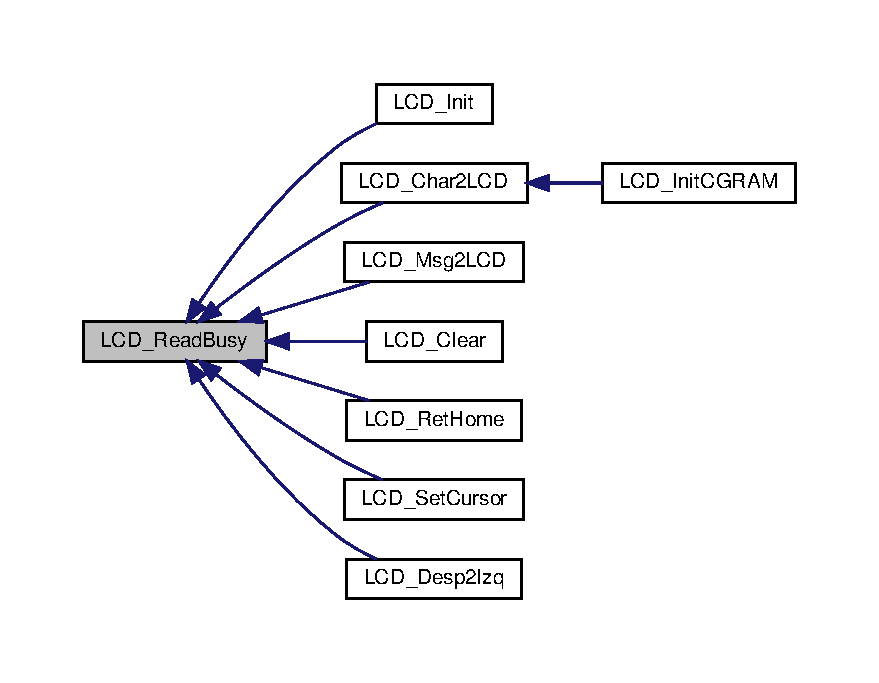
\includegraphics[width=350pt]{d8/dd6/FW__LCD_8c_a72115baa02a7c5fb1c015ac3cea2308d_icgraph}
\end{center}
\end{figure}
\mbox{\Hypertarget{FW__LCD_8c_a9d705e44e019897df3cf52334f6d2083}\label{FW__LCD_8c_a9d705e44e019897df3cf52334f6d2083}} 
\index{F\+W\+\_\+\+L\+C\+D.\+c@{F\+W\+\_\+\+L\+C\+D.\+c}!L\+C\+D\+\_\+\+Tic\+L\+CD@{L\+C\+D\+\_\+\+Tic\+L\+CD}}
\index{L\+C\+D\+\_\+\+Tic\+L\+CD@{L\+C\+D\+\_\+\+Tic\+L\+CD}!F\+W\+\_\+\+L\+C\+D.\+c@{F\+W\+\_\+\+L\+C\+D.\+c}}
\subsubsection{\texorpdfstring{L\+C\+D\+\_\+\+Tic\+L\+C\+D()}{LCD\_TicLCD()}}
{\footnotesize\ttfamily void L\+C\+D\+\_\+\+Tic\+L\+CD (\begin{DoxyParamCaption}\item[{void}]{ }\end{DoxyParamCaption})}



Rutina necesaria para el fncionamiento del m�dulo. 

Esta rutina se debe llama desde la interrupci�n de timer cada 1mS \begin{DoxyAuthor}{Autor}
Esteban Lemos 
\end{DoxyAuthor}
\begin{DoxyDate}{Fecha}

\end{DoxyDate}


Definición en la línea 172 del archivo F\+W\+\_\+\+L\+C\+D.\+c.

\mbox{\Hypertarget{FW__LCD_8c_aa0b64783f3a2f265b3bda0b9d92d7d89}\label{FW__LCD_8c_aa0b64783f3a2f265b3bda0b9d92d7d89}} 
\index{F\+W\+\_\+\+L\+C\+D.\+c@{F\+W\+\_\+\+L\+C\+D.\+c}!L\+C\+D\+\_\+\+Write@{L\+C\+D\+\_\+\+Write}}
\index{L\+C\+D\+\_\+\+Write@{L\+C\+D\+\_\+\+Write}!F\+W\+\_\+\+L\+C\+D.\+c@{F\+W\+\_\+\+L\+C\+D.\+c}}
\subsubsection{\texorpdfstring{L\+C\+D\+\_\+\+Write()}{LCD\_Write()}}
{\footnotesize\ttfamily void L\+C\+D\+\_\+\+Write (\begin{DoxyParamCaption}\item[{\hyperlink{Tdatos_8h_aba7bc1797add20fe3efdf37ced1182c5}{uint8\+\_\+t}}]{dato }\end{DoxyParamCaption})}



Se encarga de escribir un dato en bus de a un nibble por vez. 

Se encarga de escribir un dato en bus de a un nibble por vez para poder trabajar en 4 bits. \begin{DoxyAuthor}{Autor}
Esteban Lemos 
\end{DoxyAuthor}
\begin{DoxyDate}{Fecha}

\end{DoxyDate}

\begin{DoxyParams}[1]{Parámetros}
\mbox{\tt in}  & {\em Recive} & el dato a enviar al L\+CD \\
\hline
\end{DoxyParams}


Definición en la línea 138 del archivo F\+W\+\_\+\+L\+C\+D.\+c.

Gráfico de llamadas a esta función\+:\nopagebreak
\begin{figure}[H]
\begin{center}
\leavevmode
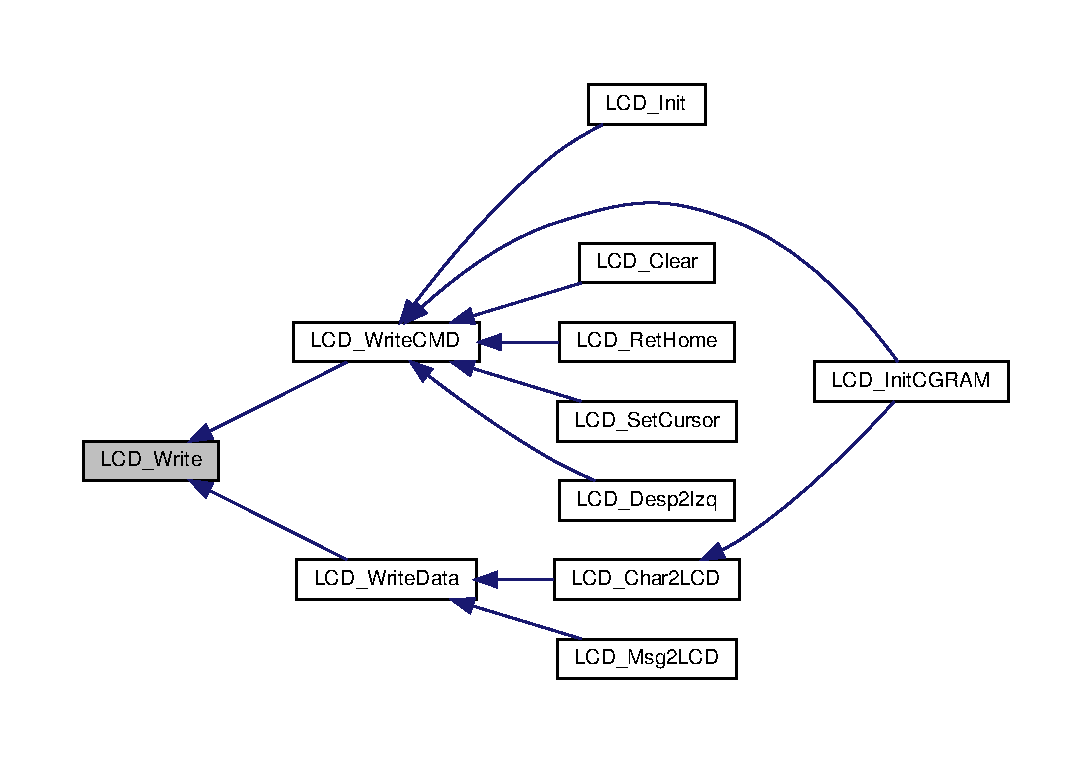
\includegraphics[width=350pt]{d8/dd6/FW__LCD_8c_aa0b64783f3a2f265b3bda0b9d92d7d89_icgraph}
\end{center}
\end{figure}
\mbox{\Hypertarget{FW__LCD_8c_a8dbf68ce3dbf3821499c9b5106838700}\label{FW__LCD_8c_a8dbf68ce3dbf3821499c9b5106838700}} 
\index{F\+W\+\_\+\+L\+C\+D.\+c@{F\+W\+\_\+\+L\+C\+D.\+c}!L\+C\+D\+\_\+\+Write\+C\+MD@{L\+C\+D\+\_\+\+Write\+C\+MD}}
\index{L\+C\+D\+\_\+\+Write\+C\+MD@{L\+C\+D\+\_\+\+Write\+C\+MD}!F\+W\+\_\+\+L\+C\+D.\+c@{F\+W\+\_\+\+L\+C\+D.\+c}}
\subsubsection{\texorpdfstring{L\+C\+D\+\_\+\+Write\+C\+M\+D()}{LCD\_WriteCMD()}}
{\footnotesize\ttfamily void L\+C\+D\+\_\+\+Write\+C\+MD (\begin{DoxyParamCaption}\item[{\hyperlink{Tdatos_8h_aba7bc1797add20fe3efdf37ced1182c5}{uint8\+\_\+t}}]{comando }\end{DoxyParamCaption})}



Definición en la línea 122 del archivo F\+W\+\_\+\+L\+C\+D.\+c.

Gráfico de llamadas a esta función\+:\nopagebreak
\begin{figure}[H]
\begin{center}
\leavevmode
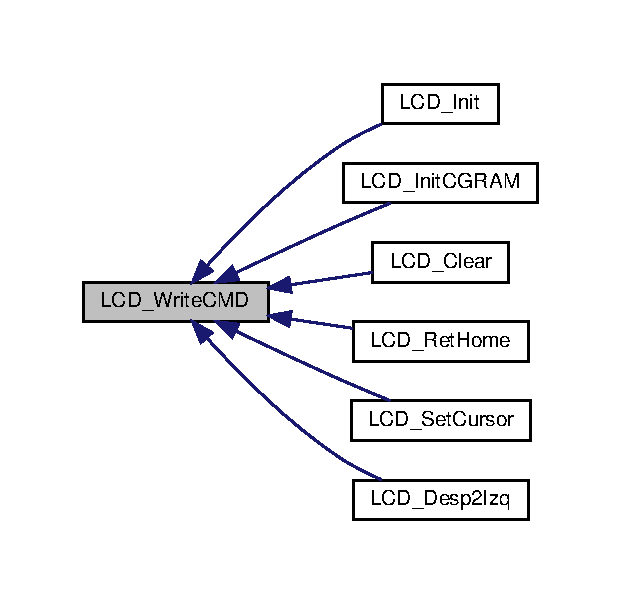
\includegraphics[width=298pt]{d8/dd6/FW__LCD_8c_a8dbf68ce3dbf3821499c9b5106838700_icgraph}
\end{center}
\end{figure}
\mbox{\Hypertarget{FW__LCD_8c_a5ced9cb01df0ef6d721dec73ae29b11b}\label{FW__LCD_8c_a5ced9cb01df0ef6d721dec73ae29b11b}} 
\index{F\+W\+\_\+\+L\+C\+D.\+c@{F\+W\+\_\+\+L\+C\+D.\+c}!L\+C\+D\+\_\+\+Write\+Data@{L\+C\+D\+\_\+\+Write\+Data}}
\index{L\+C\+D\+\_\+\+Write\+Data@{L\+C\+D\+\_\+\+Write\+Data}!F\+W\+\_\+\+L\+C\+D.\+c@{F\+W\+\_\+\+L\+C\+D.\+c}}
\subsubsection{\texorpdfstring{L\+C\+D\+\_\+\+Write\+Data()}{LCD\_WriteData()}}
{\footnotesize\ttfamily void L\+C\+D\+\_\+\+Write\+Data (\begin{DoxyParamCaption}\item[{\hyperlink{Tdatos_8h_aba7bc1797add20fe3efdf37ced1182c5}{uint8\+\_\+t}}]{dato }\end{DoxyParamCaption})}



Definición en la línea 157 del archivo F\+W\+\_\+\+L\+C\+D.\+c.

Gráfico de llamadas a esta función\+:\nopagebreak
\begin{figure}[H]
\begin{center}
\leavevmode
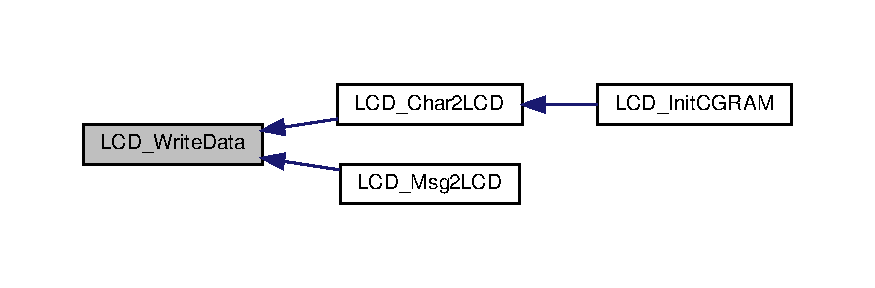
\includegraphics[width=350pt]{d8/dd6/FW__LCD_8c_a5ced9cb01df0ef6d721dec73ae29b11b_icgraph}
\end{center}
\end{figure}


\subsection{Documentación de las variables}
\mbox{\Hypertarget{FW__LCD_8c_a3dd55c3be6a5452edf6e1d8b8b90213f}\label{FW__LCD_8c_a3dd55c3be6a5452edf6e1d8b8b90213f}} 
\index{F\+W\+\_\+\+L\+C\+D.\+c@{F\+W\+\_\+\+L\+C\+D.\+c}!L\+C\+D\+\_\+\+Tout@{L\+C\+D\+\_\+\+Tout}}
\index{L\+C\+D\+\_\+\+Tout@{L\+C\+D\+\_\+\+Tout}!F\+W\+\_\+\+L\+C\+D.\+c@{F\+W\+\_\+\+L\+C\+D.\+c}}
\subsubsection{\texorpdfstring{L\+C\+D\+\_\+\+Tout}{LCD\_Tout}}
{\footnotesize\ttfamily volatile \hyperlink{Tdatos_8h_aba7bc1797add20fe3efdf37ced1182c5}{uint8\+\_\+t} L\+C\+D\+\_\+\+Tout = 0}



Definición en la línea 68 del archivo F\+W\+\_\+\+L\+C\+D.\+c.


\hypertarget{FW__PWM_8c}{}\section{Referencia del Archivo Firmware\+\_\+\+Driver/\+F\+W\+\_\+\+P\+WM.c}
\label{FW__PWM_8c}\index{Firmware\+\_\+\+Driver/\+F\+W\+\_\+\+P\+W\+M.\+c@{Firmware\+\_\+\+Driver/\+F\+W\+\_\+\+P\+W\+M.\+c}}
{\ttfamily \#include $<$xc.\+h$>$}\newline
{\ttfamily \#include \char`\"{}P\+W\+M.\+h\char`\"{}}\newline
Dependencia gráfica adjunta para F\+W\+\_\+\+P\+W\+M.\+c\+:\nopagebreak
\begin{figure}[H]
\begin{center}
\leavevmode
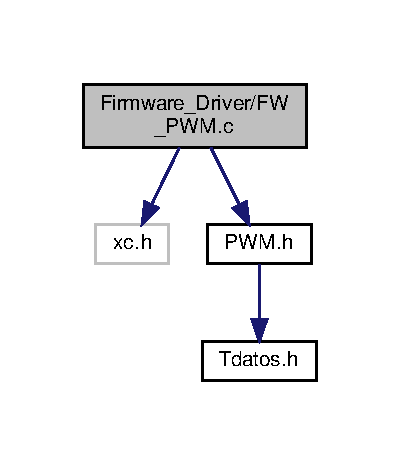
\includegraphics[width=192pt]{d6/d51/FW__PWM_8c__incl}
\end{center}
\end{figure}
\subsection*{Funciones}
\begin{DoxyCompactItemize}
\item 
void \hyperlink{FW__PWM_8c_a25de8920266a6c9f55c9b84784243228}{P\+W\+M\+\_\+\+Calc\+Frec} (void)
\end{DoxyCompactItemize}
\subsection*{Variables}
\begin{DoxyCompactItemize}
\item 
\hyperlink{Tdatos_8h_adf4d876453337156dde61095e1f20223}{uint16\+\_\+t} \hyperlink{FW__PWM_8c_a8ee991cf7d3558ce62bbc1440560d014}{P\+W\+M\+\_\+\+Medio\+Periodo\+Set} = 0
\item 
\hyperlink{Tdatos_8h_aba7bc1797add20fe3efdf37ced1182c5}{uint8\+\_\+t} \hyperlink{FW__PWM_8c_a27017d4960691c46fe56e8021898b497}{P\+W\+M\+\_\+\+Upper\+Byte} = 0x\+FF
\item 
\hyperlink{Tdatos_8h_aba7bc1797add20fe3efdf37ced1182c5}{uint8\+\_\+t} \hyperlink{FW__PWM_8c_ac2d85b4ee7ada68975e3b6f6c2c37802}{P\+W\+M\+\_\+\+Lower\+Byte} = 0x00
\item 
\hyperlink{Tdatos_8h_aba7bc1797add20fe3efdf37ced1182c5}{uint8\+\_\+t} \hyperlink{FW__PWM_8c_abdab689370a39894be9f79e83110be3c}{P\+W\+M\+\_\+\+Offset\+Periodo} = 32
\item 
\hyperlink{Tdatos_8h_aba7bc1797add20fe3efdf37ced1182c5}{uint8\+\_\+t} \hyperlink{FW__PWM_8c_adc919b5f60108a289ad35530d26d68ac}{P\+W\+M\+\_\+\+Multiplicador} = 0
\item 
\hyperlink{Tdatos_8h_aba7bc1797add20fe3efdf37ced1182c5}{uint8\+\_\+t} \hyperlink{FW__PWM_8c_a5051e364477b0fe60bb312237fbc5b50}{P\+W\+M\+\_\+\+Multiplicador\+Set} = 0
\end{DoxyCompactItemize}


\subsection{Documentación de las funciones}
\mbox{\Hypertarget{FW__PWM_8c_a25de8920266a6c9f55c9b84784243228}\label{FW__PWM_8c_a25de8920266a6c9f55c9b84784243228}} 
\index{F\+W\+\_\+\+P\+W\+M.\+c@{F\+W\+\_\+\+P\+W\+M.\+c}!P\+W\+M\+\_\+\+Calc\+Frec@{P\+W\+M\+\_\+\+Calc\+Frec}}
\index{P\+W\+M\+\_\+\+Calc\+Frec@{P\+W\+M\+\_\+\+Calc\+Frec}!F\+W\+\_\+\+P\+W\+M.\+c@{F\+W\+\_\+\+P\+W\+M.\+c}}
\subsubsection{\texorpdfstring{P\+W\+M\+\_\+\+Calc\+Frec()}{PWM\_CalcFrec()}}
{\footnotesize\ttfamily void P\+W\+M\+\_\+\+Calc\+Frec (\begin{DoxyParamCaption}\item[{void}]{ }\end{DoxyParamCaption})}

\begin{DoxyAuthor}{Autor}
Nombre 
\end{DoxyAuthor}
\begin{DoxyDate}{Fecha}
\$\{date\} 
\end{DoxyDate}

\begin{DoxyParams}[1]{Parámetros}
\mbox{\tt in}  & {\em periodo} & \\
\hline
\mbox{\tt in}  & {\em duty} & \\
\hline
\mbox{\tt out}  & {\em void} & \\
\hline
\end{DoxyParams}


Definición en la línea 92 del archivo F\+W\+\_\+\+P\+W\+M.\+c.

Gráfico de llamadas a esta función\+:\nopagebreak
\begin{figure}[H]
\begin{center}
\leavevmode
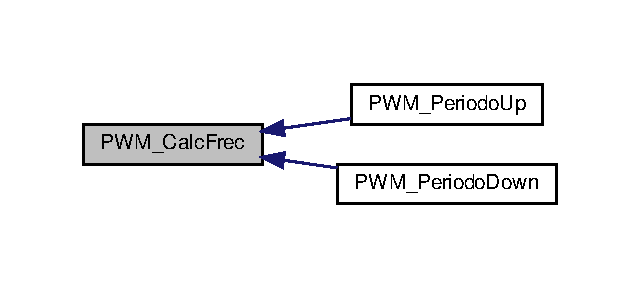
\includegraphics[width=307pt]{de/dcc/FW__PWM_8c_a25de8920266a6c9f55c9b84784243228_icgraph}
\end{center}
\end{figure}


\subsection{Documentación de las variables}
\mbox{\Hypertarget{FW__PWM_8c_ac2d85b4ee7ada68975e3b6f6c2c37802}\label{FW__PWM_8c_ac2d85b4ee7ada68975e3b6f6c2c37802}} 
\index{F\+W\+\_\+\+P\+W\+M.\+c@{F\+W\+\_\+\+P\+W\+M.\+c}!P\+W\+M\+\_\+\+Lower\+Byte@{P\+W\+M\+\_\+\+Lower\+Byte}}
\index{P\+W\+M\+\_\+\+Lower\+Byte@{P\+W\+M\+\_\+\+Lower\+Byte}!F\+W\+\_\+\+P\+W\+M.\+c@{F\+W\+\_\+\+P\+W\+M.\+c}}
\subsubsection{\texorpdfstring{P\+W\+M\+\_\+\+Lower\+Byte}{PWM\_LowerByte}}
{\footnotesize\ttfamily \hyperlink{Tdatos_8h_aba7bc1797add20fe3efdf37ced1182c5}{uint8\+\_\+t} P\+W\+M\+\_\+\+Lower\+Byte = 0x00}



Definición en la línea 66 del archivo F\+W\+\_\+\+P\+W\+M.\+c.

\mbox{\Hypertarget{FW__PWM_8c_a8ee991cf7d3558ce62bbc1440560d014}\label{FW__PWM_8c_a8ee991cf7d3558ce62bbc1440560d014}} 
\index{F\+W\+\_\+\+P\+W\+M.\+c@{F\+W\+\_\+\+P\+W\+M.\+c}!P\+W\+M\+\_\+\+Medio\+Periodo\+Set@{P\+W\+M\+\_\+\+Medio\+Periodo\+Set}}
\index{P\+W\+M\+\_\+\+Medio\+Periodo\+Set@{P\+W\+M\+\_\+\+Medio\+Periodo\+Set}!F\+W\+\_\+\+P\+W\+M.\+c@{F\+W\+\_\+\+P\+W\+M.\+c}}
\subsubsection{\texorpdfstring{P\+W\+M\+\_\+\+Medio\+Periodo\+Set}{PWM\_MedioPeriodoSet}}
{\footnotesize\ttfamily \hyperlink{Tdatos_8h_adf4d876453337156dde61095e1f20223}{uint16\+\_\+t} P\+W\+M\+\_\+\+Medio\+Periodo\+Set = 0}



Definición en la línea 64 del archivo F\+W\+\_\+\+P\+W\+M.\+c.

\mbox{\Hypertarget{FW__PWM_8c_adc919b5f60108a289ad35530d26d68ac}\label{FW__PWM_8c_adc919b5f60108a289ad35530d26d68ac}} 
\index{F\+W\+\_\+\+P\+W\+M.\+c@{F\+W\+\_\+\+P\+W\+M.\+c}!P\+W\+M\+\_\+\+Multiplicador@{P\+W\+M\+\_\+\+Multiplicador}}
\index{P\+W\+M\+\_\+\+Multiplicador@{P\+W\+M\+\_\+\+Multiplicador}!F\+W\+\_\+\+P\+W\+M.\+c@{F\+W\+\_\+\+P\+W\+M.\+c}}
\subsubsection{\texorpdfstring{P\+W\+M\+\_\+\+Multiplicador}{PWM\_Multiplicador}}
{\footnotesize\ttfamily \hyperlink{Tdatos_8h_aba7bc1797add20fe3efdf37ced1182c5}{uint8\+\_\+t} P\+W\+M\+\_\+\+Multiplicador = 0}



Definición en la línea 68 del archivo F\+W\+\_\+\+P\+W\+M.\+c.

\mbox{\Hypertarget{FW__PWM_8c_a5051e364477b0fe60bb312237fbc5b50}\label{FW__PWM_8c_a5051e364477b0fe60bb312237fbc5b50}} 
\index{F\+W\+\_\+\+P\+W\+M.\+c@{F\+W\+\_\+\+P\+W\+M.\+c}!P\+W\+M\+\_\+\+Multiplicador\+Set@{P\+W\+M\+\_\+\+Multiplicador\+Set}}
\index{P\+W\+M\+\_\+\+Multiplicador\+Set@{P\+W\+M\+\_\+\+Multiplicador\+Set}!F\+W\+\_\+\+P\+W\+M.\+c@{F\+W\+\_\+\+P\+W\+M.\+c}}
\subsubsection{\texorpdfstring{P\+W\+M\+\_\+\+Multiplicador\+Set}{PWM\_MultiplicadorSet}}
{\footnotesize\ttfamily \hyperlink{Tdatos_8h_aba7bc1797add20fe3efdf37ced1182c5}{uint8\+\_\+t} P\+W\+M\+\_\+\+Multiplicador\+Set = 0}



Definición en la línea 69 del archivo F\+W\+\_\+\+P\+W\+M.\+c.

\mbox{\Hypertarget{FW__PWM_8c_abdab689370a39894be9f79e83110be3c}\label{FW__PWM_8c_abdab689370a39894be9f79e83110be3c}} 
\index{F\+W\+\_\+\+P\+W\+M.\+c@{F\+W\+\_\+\+P\+W\+M.\+c}!P\+W\+M\+\_\+\+Offset\+Periodo@{P\+W\+M\+\_\+\+Offset\+Periodo}}
\index{P\+W\+M\+\_\+\+Offset\+Periodo@{P\+W\+M\+\_\+\+Offset\+Periodo}!F\+W\+\_\+\+P\+W\+M.\+c@{F\+W\+\_\+\+P\+W\+M.\+c}}
\subsubsection{\texorpdfstring{P\+W\+M\+\_\+\+Offset\+Periodo}{PWM\_OffsetPeriodo}}
{\footnotesize\ttfamily \hyperlink{Tdatos_8h_aba7bc1797add20fe3efdf37ced1182c5}{uint8\+\_\+t} P\+W\+M\+\_\+\+Offset\+Periodo = 32}



Definición en la línea 67 del archivo F\+W\+\_\+\+P\+W\+M.\+c.

\mbox{\Hypertarget{FW__PWM_8c_a27017d4960691c46fe56e8021898b497}\label{FW__PWM_8c_a27017d4960691c46fe56e8021898b497}} 
\index{F\+W\+\_\+\+P\+W\+M.\+c@{F\+W\+\_\+\+P\+W\+M.\+c}!P\+W\+M\+\_\+\+Upper\+Byte@{P\+W\+M\+\_\+\+Upper\+Byte}}
\index{P\+W\+M\+\_\+\+Upper\+Byte@{P\+W\+M\+\_\+\+Upper\+Byte}!F\+W\+\_\+\+P\+W\+M.\+c@{F\+W\+\_\+\+P\+W\+M.\+c}}
\subsubsection{\texorpdfstring{P\+W\+M\+\_\+\+Upper\+Byte}{PWM\_UpperByte}}
{\footnotesize\ttfamily \hyperlink{Tdatos_8h_aba7bc1797add20fe3efdf37ced1182c5}{uint8\+\_\+t} P\+W\+M\+\_\+\+Upper\+Byte = 0x\+FF}



Definición en la línea 65 del archivo F\+W\+\_\+\+P\+W\+M.\+c.


\hypertarget{FW__Teclado_8c}{}\section{Referencia del Archivo Firmware\+\_\+\+Driver/\+F\+W\+\_\+\+Teclado.c}
\label{FW__Teclado_8c}\index{Firmware\+\_\+\+Driver/\+F\+W\+\_\+\+Teclado.\+c@{Firmware\+\_\+\+Driver/\+F\+W\+\_\+\+Teclado.\+c}}
{\ttfamily \#include \char`\"{}F\+W\+\_\+\+Teclado.\+h\char`\"{}}\newline
Dependencia gráfica adjunta para F\+W\+\_\+\+Teclado.\+c\+:\nopagebreak
\begin{figure}[H]
\begin{center}
\leavevmode
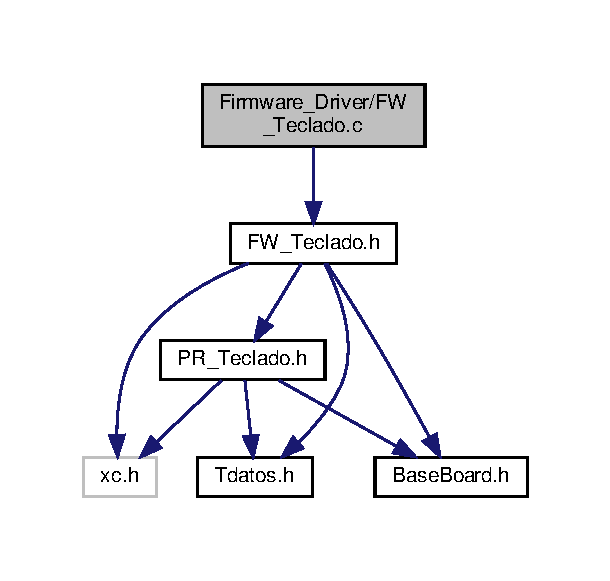
\includegraphics[width=293pt]{d7/d3b/FW__Teclado_8c__incl}
\end{center}
\end{figure}
\subsection*{Funciones}
\begin{DoxyCompactItemize}
\item 
void \hyperlink{FW__Teclado_8c_a64caa519224486b8d93e72a92156679a}{T\+D\+O\+\_\+\+Marca\+Tecla} (void)
\item 
void \hyperlink{FW__Teclado_8c_a0baf84f98398f0ba3fa364fec157e136}{T\+D\+O\+\_\+\+Tic} (void)
\item 
void \hyperlink{FW__Teclado_8c_a72699b8ff8dd75ac13b3fc778bfe365e}{T\+D\+O\+\_\+\+Little\+Delay} (void)
\begin{DoxyCompactList}\small\item\em demora breve \end{DoxyCompactList}\end{DoxyCompactItemize}
\subsection*{Variables}
\begin{DoxyCompactItemize}
\item 
volatile \hyperlink{Tdatos_8h_aba7bc1797add20fe3efdf37ced1182c5}{uint8\+\_\+t} \hyperlink{FW__Teclado_8c_ab75acb8d09061e3b294d9c0c435e8514}{T\+D\+O\+\_\+fila}
\item 
volatile \hyperlink{Tdatos_8h_aba7bc1797add20fe3efdf37ced1182c5}{uint8\+\_\+t} \hyperlink{FW__Teclado_8c_ab846ff016af943e75c8eba19dcf42b8c}{T\+D\+O\+\_\+col}
\item 
volatile \hyperlink{Tdatos_8h_aba7bc1797add20fe3efdf37ced1182c5}{uint8\+\_\+t} \hyperlink{FW__Teclado_8c_a49975b416d0c0b1ffb4d872eb258950e}{T\+D\+O\+\_\+flag\+\_\+kb}
\item 
volatile \hyperlink{Tdatos_8h_aba7bc1797add20fe3efdf37ced1182c5}{uint8\+\_\+t} \hyperlink{FW__Teclado_8c_abe39f361a76120416e542e6402704c48}{T\+D\+O\+\_\+delay\+\_\+kb}
\end{DoxyCompactItemize}


\subsection{Documentación de las funciones}
\mbox{\Hypertarget{FW__Teclado_8c_a72699b8ff8dd75ac13b3fc778bfe365e}\label{FW__Teclado_8c_a72699b8ff8dd75ac13b3fc778bfe365e}} 
\index{F\+W\+\_\+\+Teclado.\+c@{F\+W\+\_\+\+Teclado.\+c}!T\+D\+O\+\_\+\+Little\+Delay@{T\+D\+O\+\_\+\+Little\+Delay}}
\index{T\+D\+O\+\_\+\+Little\+Delay@{T\+D\+O\+\_\+\+Little\+Delay}!F\+W\+\_\+\+Teclado.\+c@{F\+W\+\_\+\+Teclado.\+c}}
\subsubsection{\texorpdfstring{T\+D\+O\+\_\+\+Little\+Delay()}{TDO\_LittleDelay()}}
{\footnotesize\ttfamily void T\+D\+O\+\_\+\+Little\+Delay (\begin{DoxyParamCaption}\item[{void}]{ }\end{DoxyParamCaption})}



demora breve 

\begin{DoxyAuthor}{Autor}
Esteban Lemos 
\end{DoxyAuthor}
\begin{DoxyDate}{Fecha}

\end{DoxyDate}


Definición en la línea 120 del archivo F\+W\+\_\+\+Teclado.\+c.

Gráfico de llamadas a esta función\+:\nopagebreak
\begin{figure}[H]
\begin{center}
\leavevmode
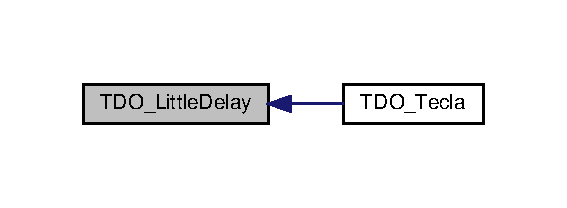
\includegraphics[width=272pt]{df/daa/FW__Teclado_8c_a72699b8ff8dd75ac13b3fc778bfe365e_icgraph}
\end{center}
\end{figure}
\mbox{\Hypertarget{FW__Teclado_8c_a64caa519224486b8d93e72a92156679a}\label{FW__Teclado_8c_a64caa519224486b8d93e72a92156679a}} 
\index{F\+W\+\_\+\+Teclado.\+c@{F\+W\+\_\+\+Teclado.\+c}!T\+D\+O\+\_\+\+Marca\+Tecla@{T\+D\+O\+\_\+\+Marca\+Tecla}}
\index{T\+D\+O\+\_\+\+Marca\+Tecla@{T\+D\+O\+\_\+\+Marca\+Tecla}!F\+W\+\_\+\+Teclado.\+c@{F\+W\+\_\+\+Teclado.\+c}}
\subsubsection{\texorpdfstring{T\+D\+O\+\_\+\+Marca\+Tecla()}{TDO\_MarcaTecla()}}
{\footnotesize\ttfamily void T\+D\+O\+\_\+\+Marca\+Tecla (\begin{DoxyParamCaption}\item[{void}]{ }\end{DoxyParamCaption})}

Funcion para uso de teclado la misma se incluye en la interrupci�n de teclado. La misma pone un estado alto el flag que indica el evento de teclado para otros micros o placas \begin{DoxyAuthor}{Autor}
Esteban Lemos 
\end{DoxyAuthor}
\begin{DoxyDate}{Fecha}

\end{DoxyDate}


Definición en la línea 90 del archivo F\+W\+\_\+\+Teclado.\+c.

\mbox{\Hypertarget{FW__Teclado_8c_a0baf84f98398f0ba3fa364fec157e136}\label{FW__Teclado_8c_a0baf84f98398f0ba3fa364fec157e136}} 
\index{F\+W\+\_\+\+Teclado.\+c@{F\+W\+\_\+\+Teclado.\+c}!T\+D\+O\+\_\+\+Tic@{T\+D\+O\+\_\+\+Tic}}
\index{T\+D\+O\+\_\+\+Tic@{T\+D\+O\+\_\+\+Tic}!F\+W\+\_\+\+Teclado.\+c@{F\+W\+\_\+\+Teclado.\+c}}
\subsubsection{\texorpdfstring{T\+D\+O\+\_\+\+Tic()}{TDO\_Tic()}}
{\footnotesize\ttfamily void T\+D\+O\+\_\+\+Tic (\begin{DoxyParamCaption}\item[{void}]{ }\end{DoxyParamCaption})}

Funci�n para el tratamiento del rebote se incluye en la interrupci�n del timer , que deber� estar configurado en 1ms un milisegundo. La misma decrementa una variable que se encarga de definir los tiempos de estabilidad y as� evitar el rebote. \begin{DoxyAuthor}{Autor}
Esteban Lemos 
\end{DoxyAuthor}
\begin{DoxyDate}{Fecha}

\end{DoxyDate}


Definición en la línea 109 del archivo F\+W\+\_\+\+Teclado.\+c.



\subsection{Documentación de las variables}
\mbox{\Hypertarget{FW__Teclado_8c_ab846ff016af943e75c8eba19dcf42b8c}\label{FW__Teclado_8c_ab846ff016af943e75c8eba19dcf42b8c}} 
\index{F\+W\+\_\+\+Teclado.\+c@{F\+W\+\_\+\+Teclado.\+c}!T\+D\+O\+\_\+col@{T\+D\+O\+\_\+col}}
\index{T\+D\+O\+\_\+col@{T\+D\+O\+\_\+col}!F\+W\+\_\+\+Teclado.\+c@{F\+W\+\_\+\+Teclado.\+c}}
\subsubsection{\texorpdfstring{T\+D\+O\+\_\+col}{TDO\_col}}
{\footnotesize\ttfamily volatile \hyperlink{Tdatos_8h_aba7bc1797add20fe3efdf37ced1182c5}{uint8\+\_\+t} T\+D\+O\+\_\+col}



Definición en la línea 62 del archivo F\+W\+\_\+\+Init\+Teclado.\+c.

\mbox{\Hypertarget{FW__Teclado_8c_abe39f361a76120416e542e6402704c48}\label{FW__Teclado_8c_abe39f361a76120416e542e6402704c48}} 
\index{F\+W\+\_\+\+Teclado.\+c@{F\+W\+\_\+\+Teclado.\+c}!T\+D\+O\+\_\+delay\+\_\+kb@{T\+D\+O\+\_\+delay\+\_\+kb}}
\index{T\+D\+O\+\_\+delay\+\_\+kb@{T\+D\+O\+\_\+delay\+\_\+kb}!F\+W\+\_\+\+Teclado.\+c@{F\+W\+\_\+\+Teclado.\+c}}
\subsubsection{\texorpdfstring{T\+D\+O\+\_\+delay\+\_\+kb}{TDO\_delay\_kb}}
{\footnotesize\ttfamily volatile \hyperlink{Tdatos_8h_aba7bc1797add20fe3efdf37ced1182c5}{uint8\+\_\+t} T\+D\+O\+\_\+delay\+\_\+kb}



Definición en la línea 64 del archivo F\+W\+\_\+\+Init\+Teclado.\+c.

\mbox{\Hypertarget{FW__Teclado_8c_ab75acb8d09061e3b294d9c0c435e8514}\label{FW__Teclado_8c_ab75acb8d09061e3b294d9c0c435e8514}} 
\index{F\+W\+\_\+\+Teclado.\+c@{F\+W\+\_\+\+Teclado.\+c}!T\+D\+O\+\_\+fila@{T\+D\+O\+\_\+fila}}
\index{T\+D\+O\+\_\+fila@{T\+D\+O\+\_\+fila}!F\+W\+\_\+\+Teclado.\+c@{F\+W\+\_\+\+Teclado.\+c}}
\subsubsection{\texorpdfstring{T\+D\+O\+\_\+fila}{TDO\_fila}}
{\footnotesize\ttfamily volatile \hyperlink{Tdatos_8h_aba7bc1797add20fe3efdf37ced1182c5}{uint8\+\_\+t} T\+D\+O\+\_\+fila}



Definición en la línea 61 del archivo F\+W\+\_\+\+Init\+Teclado.\+c.

\mbox{\Hypertarget{FW__Teclado_8c_a49975b416d0c0b1ffb4d872eb258950e}\label{FW__Teclado_8c_a49975b416d0c0b1ffb4d872eb258950e}} 
\index{F\+W\+\_\+\+Teclado.\+c@{F\+W\+\_\+\+Teclado.\+c}!T\+D\+O\+\_\+flag\+\_\+kb@{T\+D\+O\+\_\+flag\+\_\+kb}}
\index{T\+D\+O\+\_\+flag\+\_\+kb@{T\+D\+O\+\_\+flag\+\_\+kb}!F\+W\+\_\+\+Teclado.\+c@{F\+W\+\_\+\+Teclado.\+c}}
\subsubsection{\texorpdfstring{T\+D\+O\+\_\+flag\+\_\+kb}{TDO\_flag\_kb}}
{\footnotesize\ttfamily volatile \hyperlink{Tdatos_8h_aba7bc1797add20fe3efdf37ced1182c5}{uint8\+\_\+t} T\+D\+O\+\_\+flag\+\_\+kb}



Definición en la línea 63 del archivo F\+W\+\_\+\+Init\+Teclado.\+c.


\hypertarget{FW__InitEncoderIncremetnal_8c}{}\section{Referencia del Archivo Firmware\+\_\+\+Init/\+F\+W\+\_\+\+Init\+Encoder\+Incremetnal.c}
\label{FW__InitEncoderIncremetnal_8c}\index{Firmware\+\_\+\+Init/\+F\+W\+\_\+\+Init\+Encoder\+Incremetnal.\+c@{Firmware\+\_\+\+Init/\+F\+W\+\_\+\+Init\+Encoder\+Incremetnal.\+c}}
{\ttfamily \#include $<$xc.\+h$>$}\newline
{\ttfamily \#include \char`\"{}Tdatos.\+h\char`\"{}}\newline
{\ttfamily \#include \char`\"{}Base\+Board.\+h\char`\"{}}\newline
{\ttfamily \#include \char`\"{}Encoder\+Incremental.\+h\char`\"{}}\newline
Dependencia gráfica adjunta para F\+W\+\_\+\+Init\+Encoder\+Incremetnal.\+c\+:\nopagebreak
\begin{figure}[H]
\begin{center}
\leavevmode
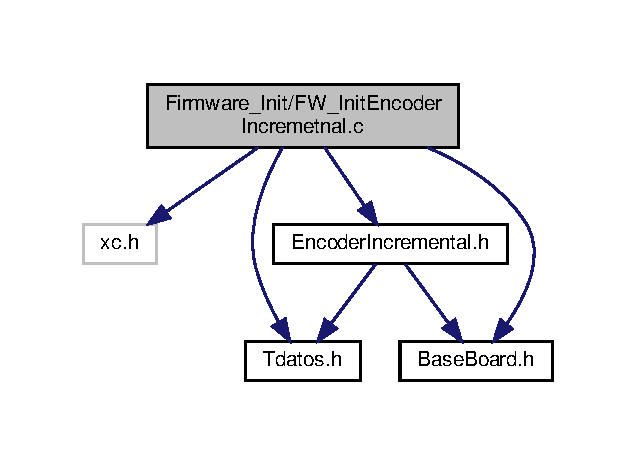
\includegraphics[width=305pt]{df/d6c/FW__InitEncoderIncremetnal_8c__incl}
\end{center}
\end{figure}
\subsection*{Funciones}
\begin{DoxyCompactItemize}
\item 
void \hyperlink{FW__InitEncoderIncremetnal_8c_a1f92e3491d1d96007589f41b5eb03fe7}{E\+D\+E\+R\+\_\+\+Init} (\hyperlink{Tdatos_8h_aba7bc1797add20fe3efdf37ced1182c5}{uint8\+\_\+t} set\+M\+AX, \hyperlink{Tdatos_8h_aba7bc1797add20fe3efdf37ced1182c5}{uint8\+\_\+t} set\+Min)
\begin{DoxyCompactList}\small\item\em Funcion necesaria para inicializar el encoder, en la misma se define el rango del encoder. \end{DoxyCompactList}\end{DoxyCompactItemize}
\subsection*{Variables}
\begin{DoxyCompactItemize}
\item 
volatile \hyperlink{Tdatos_8h_aba7bc1797add20fe3efdf37ced1182c5}{uint8\+\_\+t} \hyperlink{FW__InitEncoderIncremetnal_8c_acba4a26c0330eb8f52158e306351fd67}{E\+D\+E\+R\+\_\+\+Maximo} = 0
\item 
volatile \hyperlink{Tdatos_8h_aba7bc1797add20fe3efdf37ced1182c5}{uint8\+\_\+t} \hyperlink{FW__InitEncoderIncremetnal_8c_a60645d94d942d68dd1c4a5d039df5860}{E\+D\+E\+R\+\_\+\+Minimo} = 0
\end{DoxyCompactItemize}


\subsection{Documentación de las funciones}
\mbox{\Hypertarget{FW__InitEncoderIncremetnal_8c_a1f92e3491d1d96007589f41b5eb03fe7}\label{FW__InitEncoderIncremetnal_8c_a1f92e3491d1d96007589f41b5eb03fe7}} 
\index{F\+W\+\_\+\+Init\+Encoder\+Incremetnal.\+c@{F\+W\+\_\+\+Init\+Encoder\+Incremetnal.\+c}!E\+D\+E\+R\+\_\+\+Init@{E\+D\+E\+R\+\_\+\+Init}}
\index{E\+D\+E\+R\+\_\+\+Init@{E\+D\+E\+R\+\_\+\+Init}!F\+W\+\_\+\+Init\+Encoder\+Incremetnal.\+c@{F\+W\+\_\+\+Init\+Encoder\+Incremetnal.\+c}}
\subsubsection{\texorpdfstring{E\+D\+E\+R\+\_\+\+Init()}{EDER\_Init()}}
{\footnotesize\ttfamily void E\+D\+E\+R\+\_\+\+Init (\begin{DoxyParamCaption}\item[{\hyperlink{Tdatos_8h_aba7bc1797add20fe3efdf37ced1182c5}{uint8\+\_\+t}}]{set\+M\+AX,  }\item[{\hyperlink{Tdatos_8h_aba7bc1797add20fe3efdf37ced1182c5}{uint8\+\_\+t}}]{set\+Min }\end{DoxyParamCaption})}



Funcion necesaria para inicializar el encoder, en la misma se define el rango del encoder. 

\begin{DoxyAuthor}{Autor}

\end{DoxyAuthor}
\begin{DoxyDate}{Fecha}

\end{DoxyDate}

\begin{DoxyParams}[1]{Parámetros}
\mbox{\tt in}  & {\em set\+M\+AX} & necesario para definir la posicion maxima \\
\hline
\mbox{\tt in}  & {\em set\+Min} & necesario para definir la posicion minima \\
\hline
\mbox{\tt out}  & {\em void} & \\
\hline
\end{DoxyParams}


Definición en la línea 93 del archivo F\+W\+\_\+\+Init\+Encoder\+Incremetnal.\+c.



\subsection{Documentación de las variables}
\mbox{\Hypertarget{FW__InitEncoderIncremetnal_8c_acba4a26c0330eb8f52158e306351fd67}\label{FW__InitEncoderIncremetnal_8c_acba4a26c0330eb8f52158e306351fd67}} 
\index{F\+W\+\_\+\+Init\+Encoder\+Incremetnal.\+c@{F\+W\+\_\+\+Init\+Encoder\+Incremetnal.\+c}!E\+D\+E\+R\+\_\+\+Maximo@{E\+D\+E\+R\+\_\+\+Maximo}}
\index{E\+D\+E\+R\+\_\+\+Maximo@{E\+D\+E\+R\+\_\+\+Maximo}!F\+W\+\_\+\+Init\+Encoder\+Incremetnal.\+c@{F\+W\+\_\+\+Init\+Encoder\+Incremetnal.\+c}}
\subsubsection{\texorpdfstring{E\+D\+E\+R\+\_\+\+Maximo}{EDER\_Maximo}}
{\footnotesize\ttfamily volatile \hyperlink{Tdatos_8h_aba7bc1797add20fe3efdf37ced1182c5}{uint8\+\_\+t} E\+D\+E\+R\+\_\+\+Maximo = 0}



Definición en la línea 68 del archivo F\+W\+\_\+\+Init\+Encoder\+Incremetnal.\+c.

\mbox{\Hypertarget{FW__InitEncoderIncremetnal_8c_a60645d94d942d68dd1c4a5d039df5860}\label{FW__InitEncoderIncremetnal_8c_a60645d94d942d68dd1c4a5d039df5860}} 
\index{F\+W\+\_\+\+Init\+Encoder\+Incremetnal.\+c@{F\+W\+\_\+\+Init\+Encoder\+Incremetnal.\+c}!E\+D\+E\+R\+\_\+\+Minimo@{E\+D\+E\+R\+\_\+\+Minimo}}
\index{E\+D\+E\+R\+\_\+\+Minimo@{E\+D\+E\+R\+\_\+\+Minimo}!F\+W\+\_\+\+Init\+Encoder\+Incremetnal.\+c@{F\+W\+\_\+\+Init\+Encoder\+Incremetnal.\+c}}
\subsubsection{\texorpdfstring{E\+D\+E\+R\+\_\+\+Minimo}{EDER\_Minimo}}
{\footnotesize\ttfamily volatile \hyperlink{Tdatos_8h_aba7bc1797add20fe3efdf37ced1182c5}{uint8\+\_\+t} E\+D\+E\+R\+\_\+\+Minimo = 0}



Definición en la línea 69 del archivo F\+W\+\_\+\+Init\+Encoder\+Incremetnal.\+c.


\hypertarget{FW__InitKit_8c}{}\section{Referencia del Archivo Firmware\+\_\+\+Init/\+F\+W\+\_\+\+Init\+Kit.c}
\label{FW__InitKit_8c}\index{Firmware\+\_\+\+Init/\+F\+W\+\_\+\+Init\+Kit.\+c@{Firmware\+\_\+\+Init/\+F\+W\+\_\+\+Init\+Kit.\+c}}
{\ttfamily \#include \char`\"{}F\+W\+\_\+\+Init\+Kit.\+h\char`\"{}}\newline
Dependencia gráfica adjunta para F\+W\+\_\+\+Init\+Kit.\+c\+:\nopagebreak
\begin{figure}[H]
\begin{center}
\leavevmode
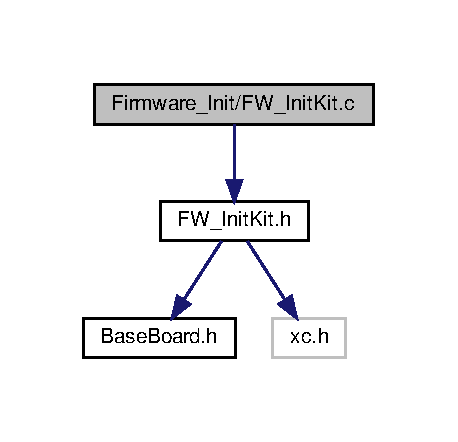
\includegraphics[width=220pt]{de/da1/FW__InitKit_8c__incl}
\end{center}
\end{figure}
\subsection*{Funciones}
\begin{DoxyCompactItemize}
\item 
void \hyperlink{FW__InitKit_8c_a91a9e93581be29c6af058d09741ee5be}{Kit\+\_\+\+Init} (void)
\begin{DoxyCompactList}\small\item\em Inicializa el entrenador para el shield 1. \end{DoxyCompactList}\end{DoxyCompactItemize}


\subsection{Documentación de las funciones}
\mbox{\Hypertarget{FW__InitKit_8c_a91a9e93581be29c6af058d09741ee5be}\label{FW__InitKit_8c_a91a9e93581be29c6af058d09741ee5be}} 
\index{F\+W\+\_\+\+Init\+Kit.\+c@{F\+W\+\_\+\+Init\+Kit.\+c}!Kit\+\_\+\+Init@{Kit\+\_\+\+Init}}
\index{Kit\+\_\+\+Init@{Kit\+\_\+\+Init}!F\+W\+\_\+\+Init\+Kit.\+c@{F\+W\+\_\+\+Init\+Kit.\+c}}
\subsubsection{\texorpdfstring{Kit\+\_\+\+Init()}{Kit\_Init()}}
{\footnotesize\ttfamily void Kit\+\_\+\+Init (\begin{DoxyParamCaption}\item[{void}]{ }\end{DoxyParamCaption})}



Inicializa el entrenador para el shield 1. 

Inicializa todos los puertos del entrenador preparandolo para usar el display y deshabilitando los comparadores de entrada y los canales anal�gicos. Tambi�n limpia todas las salidas. \begin{DoxyAuthor}{Autor}
Esteban Lemos 
\end{DoxyAuthor}
\begin{DoxyDate}{Fecha}

\end{DoxyDate}

\begin{DoxyParams}[1]{Parámetros}
\mbox{\tt in}  & {\em void} & \\
\hline
\mbox{\tt out}  & {\em void} & \\
\hline
\end{DoxyParams}
\begin{DoxyReturn}{Devuelve}
void 
\end{DoxyReturn}


Definición en la línea 65 del archivo F\+W\+\_\+\+Init\+Kit.\+c.

Gráfico de llamadas a esta función\+:\nopagebreak
\begin{figure}[H]
\begin{center}
\leavevmode
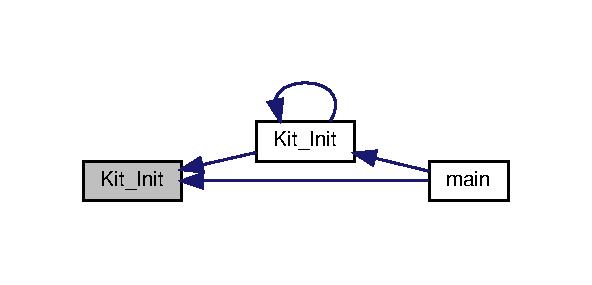
\includegraphics[width=284pt]{d6/d67/FW__InitKit_8c_a91a9e93581be29c6af058d09741ee5be_icgraph}
\end{center}
\end{figure}

\hypertarget{FW__InitLCD_8c}{}\section{Referencia del Archivo Firmware\+\_\+\+Init/\+F\+W\+\_\+\+Init\+L\+CD.c}
\label{FW__InitLCD_8c}\index{Firmware\+\_\+\+Init/\+F\+W\+\_\+\+Init\+L\+C\+D.\+c@{Firmware\+\_\+\+Init/\+F\+W\+\_\+\+Init\+L\+C\+D.\+c}}
{\ttfamily \#include \char`\"{}F\+W\+\_\+\+L\+C\+D.\+h\char`\"{}}\newline
{\ttfamily \#include \char`\"{}P\+R\+\_\+\+L\+C\+D.\+h\char`\"{}}\newline
Dependencia gráfica adjunta para F\+W\+\_\+\+Init\+L\+C\+D.\+c\+:\nopagebreak
\begin{figure}[H]
\begin{center}
\leavevmode
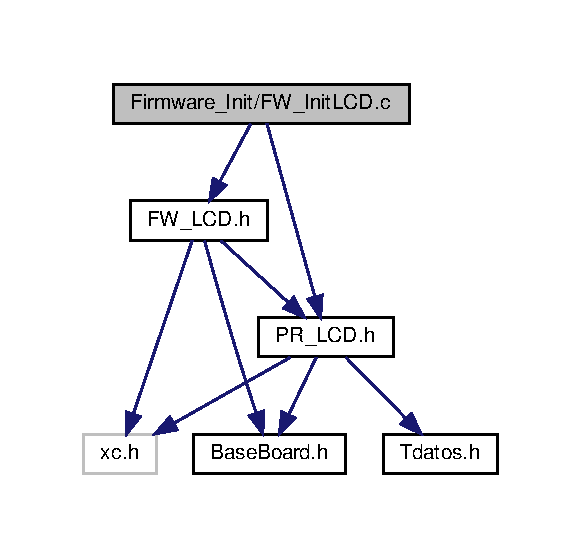
\includegraphics[width=279pt]{da/d8b/FW__InitLCD_8c__incl}
\end{center}
\end{figure}
\subsection*{defines}
\begin{DoxyCompactItemize}
\item 
\#define \hyperlink{FW__InitLCD_8c_a27fc19637a3e83d6a1836349f57beeea}{L\+C\+D\+\_\+\+E\+N\+T\+R\+A\+DA}~0x\+F0
\begin{DoxyCompactList}\small\item\em Esto es para invertir el bus de datos y poder. \end{DoxyCompactList}\item 
\#define \hyperlink{FW__InitLCD_8c_a372d8466c4b1b318bca88c3d5a454262}{L\+C\+D\+\_\+\+S\+A\+L\+I\+DA}~0x0F
\begin{DoxyCompactList}\small\item\em leer cuando necesito ver si est� busy.. \end{DoxyCompactList}\item 
\#define \hyperlink{FW__InitLCD_8c_ac8dd1658e235f174d1cabae5c438943d}{L\+C\+D\+\_\+\+B\+U\+SY}~P\+O\+R\+T\+Dbits.\+R\+D7
\begin{DoxyCompactList}\small\item\em Con estos defines me abstraigo del hardware. \end{DoxyCompactList}\item 
\#define \hyperlink{FW__InitLCD_8c_ae7fe5d669c432901d21fef38c9743dfe}{L\+C\+D\+\_\+\+B\+U\+S\+\_\+\+D\+IR}~T\+R\+I\+SD
\item 
\#define \hyperlink{FW__InitLCD_8c_aac80e54c3d1d3592462eb30e6cac6ca6}{L\+C\+D\+\_\+\+T\+R\+UE}~0x1
\item 
\#define \hyperlink{FW__InitLCD_8c_a9719ec9752a485662fafc37d1d54f98e}{L\+C\+D\+\_\+\+F\+A\+L\+SE}~0x0
\end{DoxyCompactItemize}
\subsection*{Funciones}
\begin{DoxyCompactItemize}
\item 
void \hyperlink{FW__InitLCD_8c_aa53c9d40f3aa552a9974cd55ac510cb3}{L\+C\+D\+\_\+\+Init} (void)
\begin{DoxyCompactList}\small\item\em Inicializa el L\+CD para el shield 2. \end{DoxyCompactList}\item 
void \hyperlink{FW__InitLCD_8c_ac8e88178400aaa1fc99c546c2317be14}{L\+C\+D\+\_\+\+Init\+C\+G\+R\+AM} (void)
\begin{DoxyCompactList}\small\item\em Inicializa los caracteres de la C\+G\+R\+AM para el shield 2. \end{DoxyCompactList}\end{DoxyCompactItemize}
\subsection*{Variables}
\begin{DoxyCompactItemize}
\item 
volatile \hyperlink{Tdatos_8h_aba7bc1797add20fe3efdf37ced1182c5}{uint8\+\_\+t} \hyperlink{FW__InitLCD_8c_a3dd55c3be6a5452edf6e1d8b8b90213f}{L\+C\+D\+\_\+\+Tout}
\end{DoxyCompactItemize}


\subsection{Documentación de los \textquotesingle{}defines\textquotesingle{}}
\mbox{\Hypertarget{FW__InitLCD_8c_ae7fe5d669c432901d21fef38c9743dfe}\label{FW__InitLCD_8c_ae7fe5d669c432901d21fef38c9743dfe}} 
\index{F\+W\+\_\+\+Init\+L\+C\+D.\+c@{F\+W\+\_\+\+Init\+L\+C\+D.\+c}!L\+C\+D\+\_\+\+B\+U\+S\+\_\+\+D\+IR@{L\+C\+D\+\_\+\+B\+U\+S\+\_\+\+D\+IR}}
\index{L\+C\+D\+\_\+\+B\+U\+S\+\_\+\+D\+IR@{L\+C\+D\+\_\+\+B\+U\+S\+\_\+\+D\+IR}!F\+W\+\_\+\+Init\+L\+C\+D.\+c@{F\+W\+\_\+\+Init\+L\+C\+D.\+c}}
\subsubsection{\texorpdfstring{L\+C\+D\+\_\+\+B\+U\+S\+\_\+\+D\+IR}{LCD\_BUS\_DIR}}
{\footnotesize\ttfamily \#define L\+C\+D\+\_\+\+B\+U\+S\+\_\+\+D\+IR~T\+R\+I\+SD}



Definición en la línea 53 del archivo F\+W\+\_\+\+Init\+L\+C\+D.\+c.

\mbox{\Hypertarget{FW__InitLCD_8c_ac8dd1658e235f174d1cabae5c438943d}\label{FW__InitLCD_8c_ac8dd1658e235f174d1cabae5c438943d}} 
\index{F\+W\+\_\+\+Init\+L\+C\+D.\+c@{F\+W\+\_\+\+Init\+L\+C\+D.\+c}!L\+C\+D\+\_\+\+B\+U\+SY@{L\+C\+D\+\_\+\+B\+U\+SY}}
\index{L\+C\+D\+\_\+\+B\+U\+SY@{L\+C\+D\+\_\+\+B\+U\+SY}!F\+W\+\_\+\+Init\+L\+C\+D.\+c@{F\+W\+\_\+\+Init\+L\+C\+D.\+c}}
\subsubsection{\texorpdfstring{L\+C\+D\+\_\+\+B\+U\+SY}{LCD\_BUSY}}
{\footnotesize\ttfamily \#define L\+C\+D\+\_\+\+B\+U\+SY~P\+O\+R\+T\+Dbits.\+R\+D7}



Con estos defines me abstraigo del hardware. 



Definición en la línea 52 del archivo F\+W\+\_\+\+Init\+L\+C\+D.\+c.

\mbox{\Hypertarget{FW__InitLCD_8c_a27fc19637a3e83d6a1836349f57beeea}\label{FW__InitLCD_8c_a27fc19637a3e83d6a1836349f57beeea}} 
\index{F\+W\+\_\+\+Init\+L\+C\+D.\+c@{F\+W\+\_\+\+Init\+L\+C\+D.\+c}!L\+C\+D\+\_\+\+E\+N\+T\+R\+A\+DA@{L\+C\+D\+\_\+\+E\+N\+T\+R\+A\+DA}}
\index{L\+C\+D\+\_\+\+E\+N\+T\+R\+A\+DA@{L\+C\+D\+\_\+\+E\+N\+T\+R\+A\+DA}!F\+W\+\_\+\+Init\+L\+C\+D.\+c@{F\+W\+\_\+\+Init\+L\+C\+D.\+c}}
\subsubsection{\texorpdfstring{L\+C\+D\+\_\+\+E\+N\+T\+R\+A\+DA}{LCD\_ENTRADA}}
{\footnotesize\ttfamily \#define L\+C\+D\+\_\+\+E\+N\+T\+R\+A\+DA~0x\+F0}



Esto es para invertir el bus de datos y poder. 



Definición en la línea 50 del archivo F\+W\+\_\+\+Init\+L\+C\+D.\+c.

\mbox{\Hypertarget{FW__InitLCD_8c_a9719ec9752a485662fafc37d1d54f98e}\label{FW__InitLCD_8c_a9719ec9752a485662fafc37d1d54f98e}} 
\index{F\+W\+\_\+\+Init\+L\+C\+D.\+c@{F\+W\+\_\+\+Init\+L\+C\+D.\+c}!L\+C\+D\+\_\+\+F\+A\+L\+SE@{L\+C\+D\+\_\+\+F\+A\+L\+SE}}
\index{L\+C\+D\+\_\+\+F\+A\+L\+SE@{L\+C\+D\+\_\+\+F\+A\+L\+SE}!F\+W\+\_\+\+Init\+L\+C\+D.\+c@{F\+W\+\_\+\+Init\+L\+C\+D.\+c}}
\subsubsection{\texorpdfstring{L\+C\+D\+\_\+\+F\+A\+L\+SE}{LCD\_FALSE}}
{\footnotesize\ttfamily \#define L\+C\+D\+\_\+\+F\+A\+L\+SE~0x0}



Definición en la línea 56 del archivo F\+W\+\_\+\+Init\+L\+C\+D.\+c.

\mbox{\Hypertarget{FW__InitLCD_8c_a372d8466c4b1b318bca88c3d5a454262}\label{FW__InitLCD_8c_a372d8466c4b1b318bca88c3d5a454262}} 
\index{F\+W\+\_\+\+Init\+L\+C\+D.\+c@{F\+W\+\_\+\+Init\+L\+C\+D.\+c}!L\+C\+D\+\_\+\+S\+A\+L\+I\+DA@{L\+C\+D\+\_\+\+S\+A\+L\+I\+DA}}
\index{L\+C\+D\+\_\+\+S\+A\+L\+I\+DA@{L\+C\+D\+\_\+\+S\+A\+L\+I\+DA}!F\+W\+\_\+\+Init\+L\+C\+D.\+c@{F\+W\+\_\+\+Init\+L\+C\+D.\+c}}
\subsubsection{\texorpdfstring{L\+C\+D\+\_\+\+S\+A\+L\+I\+DA}{LCD\_SALIDA}}
{\footnotesize\ttfamily \#define L\+C\+D\+\_\+\+S\+A\+L\+I\+DA~0x0F}



leer cuando necesito ver si est� busy.. 



Definición en la línea 51 del archivo F\+W\+\_\+\+Init\+L\+C\+D.\+c.

\mbox{\Hypertarget{FW__InitLCD_8c_aac80e54c3d1d3592462eb30e6cac6ca6}\label{FW__InitLCD_8c_aac80e54c3d1d3592462eb30e6cac6ca6}} 
\index{F\+W\+\_\+\+Init\+L\+C\+D.\+c@{F\+W\+\_\+\+Init\+L\+C\+D.\+c}!L\+C\+D\+\_\+\+T\+R\+UE@{L\+C\+D\+\_\+\+T\+R\+UE}}
\index{L\+C\+D\+\_\+\+T\+R\+UE@{L\+C\+D\+\_\+\+T\+R\+UE}!F\+W\+\_\+\+Init\+L\+C\+D.\+c@{F\+W\+\_\+\+Init\+L\+C\+D.\+c}}
\subsubsection{\texorpdfstring{L\+C\+D\+\_\+\+T\+R\+UE}{LCD\_TRUE}}
{\footnotesize\ttfamily \#define L\+C\+D\+\_\+\+T\+R\+UE~0x1}



Definición en la línea 55 del archivo F\+W\+\_\+\+Init\+L\+C\+D.\+c.



\subsection{Documentación de las funciones}
\mbox{\Hypertarget{FW__InitLCD_8c_aa53c9d40f3aa552a9974cd55ac510cb3}\label{FW__InitLCD_8c_aa53c9d40f3aa552a9974cd55ac510cb3}} 
\index{F\+W\+\_\+\+Init\+L\+C\+D.\+c@{F\+W\+\_\+\+Init\+L\+C\+D.\+c}!L\+C\+D\+\_\+\+Init@{L\+C\+D\+\_\+\+Init}}
\index{L\+C\+D\+\_\+\+Init@{L\+C\+D\+\_\+\+Init}!F\+W\+\_\+\+Init\+L\+C\+D.\+c@{F\+W\+\_\+\+Init\+L\+C\+D.\+c}}
\subsubsection{\texorpdfstring{L\+C\+D\+\_\+\+Init()}{LCD\_Init()}}
{\footnotesize\ttfamily void L\+C\+D\+\_\+\+Init (\begin{DoxyParamCaption}\item[{void}]{ }\end{DoxyParamCaption})}



Inicializa el L\+CD para el shield 2. 

Inicializa los puertos del entrenador necesarios para usar el display L\+CD e inicializa el L\+CD propiamente dicho. \begin{DoxyAuthor}{Autor}
Esteban Lemos 
\end{DoxyAuthor}
\begin{DoxyDate}{Fecha}

\end{DoxyDate}


Definición en la línea 120 del archivo F\+W\+\_\+\+Init\+L\+C\+D.\+c.

\mbox{\Hypertarget{FW__InitLCD_8c_ac8e88178400aaa1fc99c546c2317be14}\label{FW__InitLCD_8c_ac8e88178400aaa1fc99c546c2317be14}} 
\index{F\+W\+\_\+\+Init\+L\+C\+D.\+c@{F\+W\+\_\+\+Init\+L\+C\+D.\+c}!L\+C\+D\+\_\+\+Init\+C\+G\+R\+AM@{L\+C\+D\+\_\+\+Init\+C\+G\+R\+AM}}
\index{L\+C\+D\+\_\+\+Init\+C\+G\+R\+AM@{L\+C\+D\+\_\+\+Init\+C\+G\+R\+AM}!F\+W\+\_\+\+Init\+L\+C\+D.\+c@{F\+W\+\_\+\+Init\+L\+C\+D.\+c}}
\subsubsection{\texorpdfstring{L\+C\+D\+\_\+\+Init\+C\+G\+R\+A\+M()}{LCD\_InitCGRAM()}}
{\footnotesize\ttfamily L\+C\+D\+\_\+\+Init\+C\+G\+R\+AM (\begin{DoxyParamCaption}\item[{void}]{ }\end{DoxyParamCaption})}



Inicializa los caracteres de la C\+G\+R\+AM para el shield 2. 

Iicioaliza los caracteres creados por el usuario, solo debe llamar a esta funci�n en el main y guardar sus caracteres en la tabla L\+C\+D\+\_\+\+Characters\+C\+G\+R\+AM\mbox{[} \mbox{]} \begin{DoxyAuthor}{Autor}
Nico?as Ferragamo 
\end{DoxyAuthor}
\begin{DoxyDate}{Fecha}
1 de octubre de 2019 
\end{DoxyDate}


Definición en la línea 163 del archivo F\+W\+\_\+\+Init\+L\+C\+D.\+c.



\subsection{Documentación de las variables}
\mbox{\Hypertarget{FW__InitLCD_8c_a3dd55c3be6a5452edf6e1d8b8b90213f}\label{FW__InitLCD_8c_a3dd55c3be6a5452edf6e1d8b8b90213f}} 
\index{F\+W\+\_\+\+Init\+L\+C\+D.\+c@{F\+W\+\_\+\+Init\+L\+C\+D.\+c}!L\+C\+D\+\_\+\+Tout@{L\+C\+D\+\_\+\+Tout}}
\index{L\+C\+D\+\_\+\+Tout@{L\+C\+D\+\_\+\+Tout}!F\+W\+\_\+\+Init\+L\+C\+D.\+c@{F\+W\+\_\+\+Init\+L\+C\+D.\+c}}
\subsubsection{\texorpdfstring{L\+C\+D\+\_\+\+Tout}{LCD\_Tout}}
{\footnotesize\ttfamily volatile \hyperlink{Tdatos_8h_aba7bc1797add20fe3efdf37ced1182c5}{uint8\+\_\+t} L\+C\+D\+\_\+\+Tout}



Definición en la línea 68 del archivo F\+W\+\_\+\+L\+C\+D.\+c.


\hypertarget{FW__InitTeclado_8c}{}\section{Referencia del Archivo Firmware\+\_\+\+Init/\+F\+W\+\_\+\+Init\+Teclado.c}
\label{FW__InitTeclado_8c}\index{Firmware\+\_\+\+Init/\+F\+W\+\_\+\+Init\+Teclado.\+c@{Firmware\+\_\+\+Init/\+F\+W\+\_\+\+Init\+Teclado.\+c}}
{\ttfamily \#include \char`\"{}F\+W\+\_\+\+Teclado.\+h\char`\"{}}\newline
Dependencia gráfica adjunta para F\+W\+\_\+\+Init\+Teclado.\+c\+:\nopagebreak
\begin{figure}[H]
\begin{center}
\leavevmode
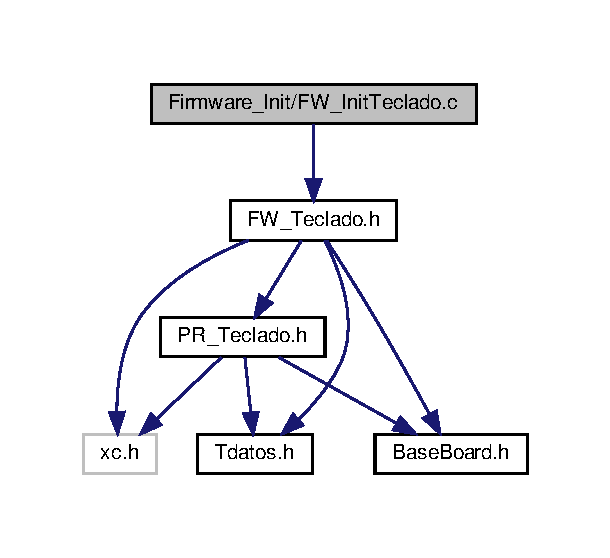
\includegraphics[width=293pt]{da/d37/FW__InitTeclado_8c__incl}
\end{center}
\end{figure}
\subsection*{Funciones}
\begin{DoxyCompactItemize}
\item 
void \hyperlink{FW__InitTeclado_8c_afca05d832c45a47fe754f4ab43de364e}{T\+D\+O\+\_\+\+Init} (void)
\begin{DoxyCompactList}\small\item\em Inicializa el puerto y las interrupciones. \end{DoxyCompactList}\end{DoxyCompactItemize}
\subsection*{Variables}
\begin{DoxyCompactItemize}
\item 
volatile \hyperlink{Tdatos_8h_aba7bc1797add20fe3efdf37ced1182c5}{uint8\+\_\+t} \hyperlink{FW__InitTeclado_8c_ab75acb8d09061e3b294d9c0c435e8514}{T\+D\+O\+\_\+fila} = \hyperlink{PR__Teclado_8h_a5c2ac6b318f743f8ff94c6c98f90f160}{T\+D\+O\+\_\+\+N\+O\+\_\+\+F\+I\+LA}
\item 
volatile \hyperlink{Tdatos_8h_aba7bc1797add20fe3efdf37ced1182c5}{uint8\+\_\+t} \hyperlink{FW__InitTeclado_8c_ab846ff016af943e75c8eba19dcf42b8c}{T\+D\+O\+\_\+col} = \hyperlink{PR__Teclado_8h_a6fa2aa72f18fdcb2f1edd6b9a4191505}{T\+D\+O\+\_\+\+N\+O\+\_\+\+C\+OL}
\item 
volatile \hyperlink{Tdatos_8h_aba7bc1797add20fe3efdf37ced1182c5}{uint8\+\_\+t} \hyperlink{FW__InitTeclado_8c_a49975b416d0c0b1ffb4d872eb258950e}{T\+D\+O\+\_\+flag\+\_\+kb} = 0
\item 
volatile \hyperlink{Tdatos_8h_aba7bc1797add20fe3efdf37ced1182c5}{uint8\+\_\+t} \hyperlink{FW__InitTeclado_8c_abe39f361a76120416e542e6402704c48}{T\+D\+O\+\_\+delay\+\_\+kb} = 0
\end{DoxyCompactItemize}


\subsection{Documentación de las funciones}
\mbox{\Hypertarget{FW__InitTeclado_8c_afca05d832c45a47fe754f4ab43de364e}\label{FW__InitTeclado_8c_afca05d832c45a47fe754f4ab43de364e}} 
\index{F\+W\+\_\+\+Init\+Teclado.\+c@{F\+W\+\_\+\+Init\+Teclado.\+c}!T\+D\+O\+\_\+\+Init@{T\+D\+O\+\_\+\+Init}}
\index{T\+D\+O\+\_\+\+Init@{T\+D\+O\+\_\+\+Init}!F\+W\+\_\+\+Init\+Teclado.\+c@{F\+W\+\_\+\+Init\+Teclado.\+c}}
\subsubsection{\texorpdfstring{T\+D\+O\+\_\+\+Init()}{TDO\_Init()}}
{\footnotesize\ttfamily void T\+D\+O\+\_\+\+Init (\begin{DoxyParamCaption}\item[{void}]{ }\end{DoxyParamCaption})}



Inicializa el puerto y las interrupciones. 

La siguiente funcion inicializa el puerto y las interrupciones. $\ast$ Para incorporar el teclado al puerto B debe de llamarse luego de\+: $\ast$ \hyperlink{FW__InitKit_8c_a91a9e93581be29c6af058d09741ee5be}{Kit\+\_\+\+Init()} y \hyperlink{FW__InitTimer_8c_a4d368e642dbd363e361c8be19cd144eb}{Tmr0\+\_\+\+Init()} I\+M\+P\+O\+R\+T\+A\+N\+T\+E!! esta funci�n solamente funciona con el Shield 1.\+3 y no debe de ser tenida en cuenta para otros micros o placas \begin{DoxyAuthor}{Autor}
Esteban Lemos 
\end{DoxyAuthor}
\begin{DoxyDate}{Fecha}

\end{DoxyDate}


Definición en la línea 94 del archivo F\+W\+\_\+\+Init\+Teclado.\+c.



\subsection{Documentación de las variables}
\mbox{\Hypertarget{FW__InitTeclado_8c_ab846ff016af943e75c8eba19dcf42b8c}\label{FW__InitTeclado_8c_ab846ff016af943e75c8eba19dcf42b8c}} 
\index{F\+W\+\_\+\+Init\+Teclado.\+c@{F\+W\+\_\+\+Init\+Teclado.\+c}!T\+D\+O\+\_\+col@{T\+D\+O\+\_\+col}}
\index{T\+D\+O\+\_\+col@{T\+D\+O\+\_\+col}!F\+W\+\_\+\+Init\+Teclado.\+c@{F\+W\+\_\+\+Init\+Teclado.\+c}}
\subsubsection{\texorpdfstring{T\+D\+O\+\_\+col}{TDO\_col}}
{\footnotesize\ttfamily volatile \hyperlink{Tdatos_8h_aba7bc1797add20fe3efdf37ced1182c5}{uint8\+\_\+t} T\+D\+O\+\_\+col = \hyperlink{PR__Teclado_8h_a6fa2aa72f18fdcb2f1edd6b9a4191505}{T\+D\+O\+\_\+\+N\+O\+\_\+\+C\+OL}}



Definición en la línea 62 del archivo F\+W\+\_\+\+Init\+Teclado.\+c.

\mbox{\Hypertarget{FW__InitTeclado_8c_abe39f361a76120416e542e6402704c48}\label{FW__InitTeclado_8c_abe39f361a76120416e542e6402704c48}} 
\index{F\+W\+\_\+\+Init\+Teclado.\+c@{F\+W\+\_\+\+Init\+Teclado.\+c}!T\+D\+O\+\_\+delay\+\_\+kb@{T\+D\+O\+\_\+delay\+\_\+kb}}
\index{T\+D\+O\+\_\+delay\+\_\+kb@{T\+D\+O\+\_\+delay\+\_\+kb}!F\+W\+\_\+\+Init\+Teclado.\+c@{F\+W\+\_\+\+Init\+Teclado.\+c}}
\subsubsection{\texorpdfstring{T\+D\+O\+\_\+delay\+\_\+kb}{TDO\_delay\_kb}}
{\footnotesize\ttfamily volatile \hyperlink{Tdatos_8h_aba7bc1797add20fe3efdf37ced1182c5}{uint8\+\_\+t} T\+D\+O\+\_\+delay\+\_\+kb = 0}



Definición en la línea 64 del archivo F\+W\+\_\+\+Init\+Teclado.\+c.

\mbox{\Hypertarget{FW__InitTeclado_8c_ab75acb8d09061e3b294d9c0c435e8514}\label{FW__InitTeclado_8c_ab75acb8d09061e3b294d9c0c435e8514}} 
\index{F\+W\+\_\+\+Init\+Teclado.\+c@{F\+W\+\_\+\+Init\+Teclado.\+c}!T\+D\+O\+\_\+fila@{T\+D\+O\+\_\+fila}}
\index{T\+D\+O\+\_\+fila@{T\+D\+O\+\_\+fila}!F\+W\+\_\+\+Init\+Teclado.\+c@{F\+W\+\_\+\+Init\+Teclado.\+c}}
\subsubsection{\texorpdfstring{T\+D\+O\+\_\+fila}{TDO\_fila}}
{\footnotesize\ttfamily volatile \hyperlink{Tdatos_8h_aba7bc1797add20fe3efdf37ced1182c5}{uint8\+\_\+t} T\+D\+O\+\_\+fila = \hyperlink{PR__Teclado_8h_a5c2ac6b318f743f8ff94c6c98f90f160}{T\+D\+O\+\_\+\+N\+O\+\_\+\+F\+I\+LA}}



Definición en la línea 61 del archivo F\+W\+\_\+\+Init\+Teclado.\+c.

\mbox{\Hypertarget{FW__InitTeclado_8c_a49975b416d0c0b1ffb4d872eb258950e}\label{FW__InitTeclado_8c_a49975b416d0c0b1ffb4d872eb258950e}} 
\index{F\+W\+\_\+\+Init\+Teclado.\+c@{F\+W\+\_\+\+Init\+Teclado.\+c}!T\+D\+O\+\_\+flag\+\_\+kb@{T\+D\+O\+\_\+flag\+\_\+kb}}
\index{T\+D\+O\+\_\+flag\+\_\+kb@{T\+D\+O\+\_\+flag\+\_\+kb}!F\+W\+\_\+\+Init\+Teclado.\+c@{F\+W\+\_\+\+Init\+Teclado.\+c}}
\subsubsection{\texorpdfstring{T\+D\+O\+\_\+flag\+\_\+kb}{TDO\_flag\_kb}}
{\footnotesize\ttfamily volatile \hyperlink{Tdatos_8h_aba7bc1797add20fe3efdf37ced1182c5}{uint8\+\_\+t} T\+D\+O\+\_\+flag\+\_\+kb = 0}



Definición en la línea 63 del archivo F\+W\+\_\+\+Init\+Teclado.\+c.


\hypertarget{FW__InitTimer_8c}{}\section{Referencia del Archivo Firmware\+\_\+\+Init/\+F\+W\+\_\+\+Init\+Timer.c}
\label{FW__InitTimer_8c}\index{Firmware\+\_\+\+Init/\+F\+W\+\_\+\+Init\+Timer.\+c@{Firmware\+\_\+\+Init/\+F\+W\+\_\+\+Init\+Timer.\+c}}
{\ttfamily \#include \char`\"{}F\+W\+\_\+\+Init\+Timer.\+h\char`\"{}}\newline
{\ttfamily \#include $<$xc.\+h$>$}\newline
{\ttfamily \#include \char`\"{}Tdatos.\+h\char`\"{}}\newline
{\ttfamily \#include \char`\"{}Base\+Board.\+h\char`\"{}}\newline
Dependencia gráfica adjunta para F\+W\+\_\+\+Init\+Timer.\+c\+:\nopagebreak
\begin{figure}[H]
\begin{center}
\leavevmode
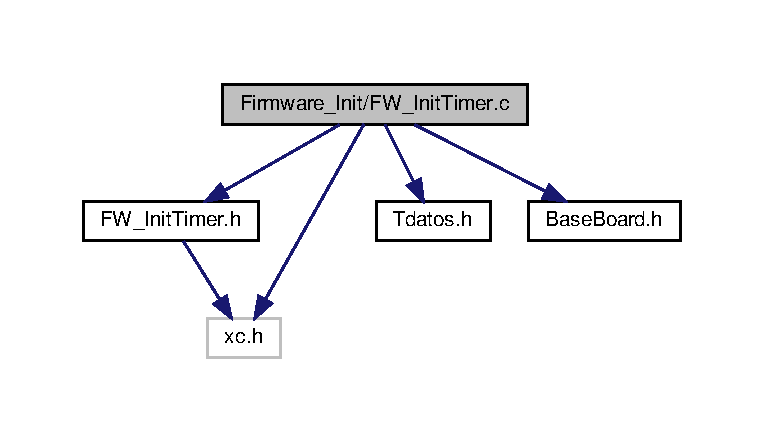
\includegraphics[width=350pt]{db/d06/FW__InitTimer_8c__incl}
\end{center}
\end{figure}
\subsection*{Funciones}
\begin{DoxyCompactItemize}
\item 
void \hyperlink{FW__InitTimer_8c_a4d368e642dbd363e361c8be19cd144eb}{Tmr0\+\_\+\+Init} (void)
\begin{DoxyCompactList}\small\item\em Inicializacion del Tmr0. \end{DoxyCompactList}\item 
void \hyperlink{FW__InitTimer_8c_aab6d953bdda9a04e181ae71ae072f95f}{Tmr1\+\_\+\+Init} (void)
\begin{DoxyCompactList}\small\item\em Inicializacion del Tmr1. \end{DoxyCompactList}\end{DoxyCompactItemize}


\subsection{Documentación de las funciones}
\mbox{\Hypertarget{FW__InitTimer_8c_a4d368e642dbd363e361c8be19cd144eb}\label{FW__InitTimer_8c_a4d368e642dbd363e361c8be19cd144eb}} 
\index{F\+W\+\_\+\+Init\+Timer.\+c@{F\+W\+\_\+\+Init\+Timer.\+c}!Tmr0\+\_\+\+Init@{Tmr0\+\_\+\+Init}}
\index{Tmr0\+\_\+\+Init@{Tmr0\+\_\+\+Init}!F\+W\+\_\+\+Init\+Timer.\+c@{F\+W\+\_\+\+Init\+Timer.\+c}}
\subsubsection{\texorpdfstring{Tmr0\+\_\+\+Init()}{Tmr0\_Init()}}
{\footnotesize\ttfamily Tmr0\+\_\+\+Init (\begin{DoxyParamCaption}\item[{void}]{ }\end{DoxyParamCaption})}



Inicializacion del Tmr0. 

Inicializa el timer 0 en 8 bits, con el prescaler en 256 y con la interrupcion activada. Esta configurado para que interrumpa cada 1.\+0022ms \begin{DoxyAuthor}{Autor}
I Esteban Lemos 
\end{DoxyAuthor}
\begin{DoxyDate}{Fecha}

\end{DoxyDate}

\begin{DoxyParams}[1]{Parámetros}
\mbox{\tt in}  & {\em void} & \\
\hline
\mbox{\tt out}  & {\em void} & \\
\hline
\end{DoxyParams}
\begin{DoxyReturn}{Devuelve}
void 
\end{DoxyReturn}


Definición en la línea 67 del archivo F\+W\+\_\+\+Init\+Timer.\+c.

Gráfico de llamadas a esta función\+:\nopagebreak
\begin{figure}[H]
\begin{center}
\leavevmode
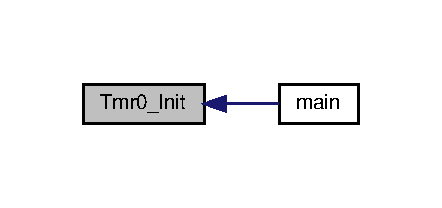
\includegraphics[width=212pt]{d2/d7e/FW__InitTimer_8c_a4d368e642dbd363e361c8be19cd144eb_icgraph}
\end{center}
\end{figure}
\mbox{\Hypertarget{FW__InitTimer_8c_aab6d953bdda9a04e181ae71ae072f95f}\label{FW__InitTimer_8c_aab6d953bdda9a04e181ae71ae072f95f}} 
\index{F\+W\+\_\+\+Init\+Timer.\+c@{F\+W\+\_\+\+Init\+Timer.\+c}!Tmr1\+\_\+\+Init@{Tmr1\+\_\+\+Init}}
\index{Tmr1\+\_\+\+Init@{Tmr1\+\_\+\+Init}!F\+W\+\_\+\+Init\+Timer.\+c@{F\+W\+\_\+\+Init\+Timer.\+c}}
\subsubsection{\texorpdfstring{Tmr1\+\_\+\+Init()}{Tmr1\_Init()}}
{\footnotesize\ttfamily Tmr1\+\_\+\+Init (\begin{DoxyParamCaption}\item[{void}]{ }\end{DoxyParamCaption})}



Inicializacion del Tmr1. 

Inicializa el timer 0 en 8 bits, con el prescaler en 256 y con la interrupcion activada. Esta configurado para que interrumpa cada 99,96 uS \begin{DoxyAuthor}{Autor}
I Esteban Lemos 
\end{DoxyAuthor}
\begin{DoxyDate}{Fecha}

\end{DoxyDate}

\begin{DoxyParams}[1]{Parámetros}
\mbox{\tt in}  & {\em void} & \\
\hline
\mbox{\tt out}  & {\em void} & \\
\hline
\end{DoxyParams}
\begin{DoxyReturn}{Devuelve}
void 
\end{DoxyReturn}


Definición en la línea 94 del archivo F\+W\+\_\+\+Init\+Timer.\+c.


\hypertarget{FW__PWMInit_8c}{}\section{Referencia del Archivo Firmware\+\_\+\+Init/\+F\+W\+\_\+\+P\+W\+M\+Init.c}
\label{FW__PWMInit_8c}\index{Firmware\+\_\+\+Init/\+F\+W\+\_\+\+P\+W\+M\+Init.\+c@{Firmware\+\_\+\+Init/\+F\+W\+\_\+\+P\+W\+M\+Init.\+c}}
{\ttfamily \#include $<$xc.\+h$>$}\newline
{\ttfamily \#include \char`\"{}P\+W\+M.\+h\char`\"{}}\newline
Dependencia gráfica adjunta para F\+W\+\_\+\+P\+W\+M\+Init.\+c\+:\nopagebreak
\begin{figure}[H]
\begin{center}
\leavevmode
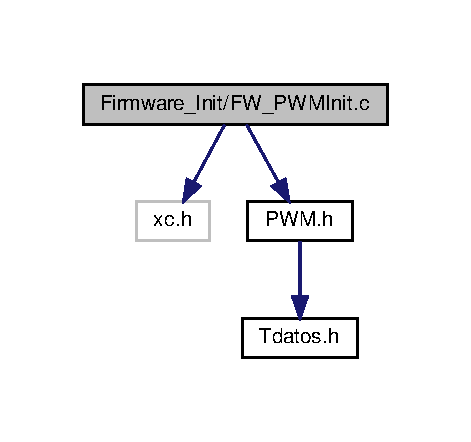
\includegraphics[width=226pt]{d7/dcd/FW__PWMInit_8c__incl}
\end{center}
\end{figure}
\subsection*{Funciones}
\begin{DoxyCompactItemize}
\item 
void \hyperlink{FW__PWMInit_8c_a2c0e86960979f0c8d21b864925b06e71}{P\+W\+M\+\_\+\+Init} (void)
\begin{DoxyCompactList}\small\item\em Inicializa los registros necesarios para usar P\+WM. \end{DoxyCompactList}\end{DoxyCompactItemize}


\subsection{Documentación de las funciones}
\mbox{\Hypertarget{FW__PWMInit_8c_a2c0e86960979f0c8d21b864925b06e71}\label{FW__PWMInit_8c_a2c0e86960979f0c8d21b864925b06e71}} 
\index{F\+W\+\_\+\+P\+W\+M\+Init.\+c@{F\+W\+\_\+\+P\+W\+M\+Init.\+c}!P\+W\+M\+\_\+\+Init@{P\+W\+M\+\_\+\+Init}}
\index{P\+W\+M\+\_\+\+Init@{P\+W\+M\+\_\+\+Init}!F\+W\+\_\+\+P\+W\+M\+Init.\+c@{F\+W\+\_\+\+P\+W\+M\+Init.\+c}}
\subsubsection{\texorpdfstring{P\+W\+M\+\_\+\+Init()}{PWM\_Init()}}
{\footnotesize\ttfamily void P\+W\+M\+\_\+\+Init (\begin{DoxyParamCaption}\item[{void}]{ }\end{DoxyParamCaption})}



Inicializa los registros necesarios para usar P\+WM. 

\begin{DoxyAuthor}{Autor}
Nombre 
\end{DoxyAuthor}
\begin{DoxyDate}{Fecha}
\$\{date\} 
\end{DoxyDate}

\begin{DoxyParams}[1]{Parámetros}
\mbox{\tt in}  & {\em void} & \\
\hline
\mbox{\tt out}  & {\em void} & \\
\hline
\end{DoxyParams}


Definición en la línea 86 del archivo F\+W\+\_\+\+P\+W\+M\+Init.\+c.


\hypertarget{FW__USARTInit_8c}{}\section{Referencia del Archivo Firmware\+\_\+\+Init/\+F\+W\+\_\+\+U\+S\+A\+R\+T\+Init.c}
\label{FW__USARTInit_8c}\index{Firmware\+\_\+\+Init/\+F\+W\+\_\+\+U\+S\+A\+R\+T\+Init.\+c@{Firmware\+\_\+\+Init/\+F\+W\+\_\+\+U\+S\+A\+R\+T\+Init.\+c}}
{\ttfamily \#include $<$xc.\+h$>$}\newline
{\ttfamily \#include \char`\"{}U\+S\+A\+R\+T.\+h\char`\"{}}\newline
Dependencia gráfica adjunta para F\+W\+\_\+\+U\+S\+A\+R\+T\+Init.\+c\+:\nopagebreak
\begin{figure}[H]
\begin{center}
\leavevmode
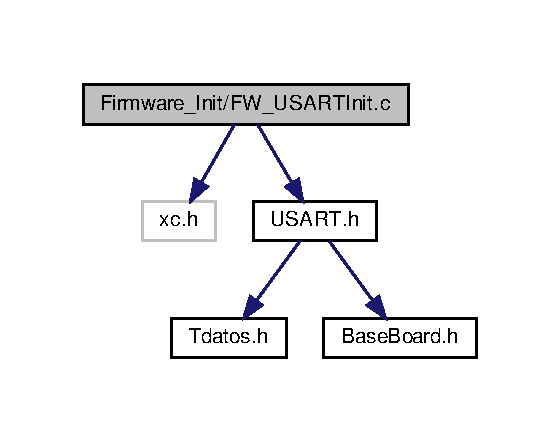
\includegraphics[width=269pt]{d6/d74/FW__USARTInit_8c__incl}
\end{center}
\end{figure}
\subsection*{Funciones}
\begin{DoxyCompactItemize}
\item 
void \hyperlink{FW__USARTInit_8c_aba398ef6d2b9f80899b2d65ca9a0fe7d}{U\+S\+A\+R\+T\+\_\+\+Init} (void)
\begin{DoxyCompactList}\small\item\em Se encarga de inicializar la U\+S\+A\+RT. \end{DoxyCompactList}\end{DoxyCompactItemize}


\subsection{Documentación de las funciones}
\mbox{\Hypertarget{FW__USARTInit_8c_aba398ef6d2b9f80899b2d65ca9a0fe7d}\label{FW__USARTInit_8c_aba398ef6d2b9f80899b2d65ca9a0fe7d}} 
\index{F\+W\+\_\+\+U\+S\+A\+R\+T\+Init.\+c@{F\+W\+\_\+\+U\+S\+A\+R\+T\+Init.\+c}!U\+S\+A\+R\+T\+\_\+\+Init@{U\+S\+A\+R\+T\+\_\+\+Init}}
\index{U\+S\+A\+R\+T\+\_\+\+Init@{U\+S\+A\+R\+T\+\_\+\+Init}!F\+W\+\_\+\+U\+S\+A\+R\+T\+Init.\+c@{F\+W\+\_\+\+U\+S\+A\+R\+T\+Init.\+c}}
\subsubsection{\texorpdfstring{U\+S\+A\+R\+T\+\_\+\+Init()}{USART\_Init()}}
{\footnotesize\ttfamily void U\+S\+A\+R\+T\+\_\+\+Init (\begin{DoxyParamCaption}\item[{void}]{ }\end{DoxyParamCaption})}



Se encarga de inicializar la U\+S\+A\+RT. 

\begin{DoxyAuthor}{Autor}

\end{DoxyAuthor}
\begin{DoxyDate}{Fecha}

\end{DoxyDate}

\begin{DoxyParams}[1]{Parámetros}
\mbox{\tt in}  & {\em void} & \\
\hline
\mbox{\tt out}  & {\em void} & \\
\hline
\end{DoxyParams}


Definición en la línea 86 del archivo F\+W\+\_\+\+U\+S\+A\+R\+T\+Init.\+c.


\hypertarget{Aplicacion_8h}{}\section{Referencia del Archivo inc/\+Aplicacion.h}
\label{Aplicacion_8h}\index{inc/\+Aplicacion.\+h@{inc/\+Aplicacion.\+h}}
{\ttfamily \#include $<$xc.\+h$>$}\newline
{\ttfamily \#include \char`\"{}Confbits.\+h\char`\"{}}\newline
{\ttfamily \#include \char`\"{}Tdatos.\+h\char`\"{}}\newline
{\ttfamily \#include \char`\"{}Base\+Board.\+h\char`\"{}}\newline
{\ttfamily \#include \char`\"{}F\+W\+\_\+\+Init\+Kit.\+h\char`\"{}}\newline
{\ttfamily \#include \char`\"{}F\+W\+\_\+\+Init\+Timer.\+h\char`\"{}}\newline
{\ttfamily \#include \char`\"{}P\+R\+\_\+\+L\+C\+D.\+h\char`\"{}}\newline
{\ttfamily \#include \char`\"{}F\+W\+\_\+\+L\+C\+D.\+h\char`\"{}}\newline
{\ttfamily \#include \char`\"{}F\+W\+\_\+\+Teclado.\+h\char`\"{}}\newline
{\ttfamily \#include \char`\"{}P\+R\+\_\+\+Teclado.\+h\char`\"{}}\newline
{\ttfamily \#include \char`\"{}Display7\+Segmentos.\+h\char`\"{}}\newline
{\ttfamily \#include \char`\"{}Entradas\+Digitales.\+h\char`\"{}}\newline
{\ttfamily \#include \char`\"{}Encoder\+Incremental.\+h\char`\"{}}\newline
{\ttfamily \#include \char`\"{}P\+W\+M.\+h\char`\"{}}\newline
{\ttfamily \#include \char`\"{}E\+E\+P\+R\+O\+M.\+h\char`\"{}}\newline
{\ttfamily \#include \char`\"{}U\+S\+A\+R\+T.\+h\char`\"{}}\newline
{\ttfamily \#include \char`\"{}P\+R\+\_\+\+A\+D\+C.\+h\char`\"{}}\newline
{\ttfamily \#include \char`\"{}Mac\+Timer.\+h\char`\"{}}\newline
Dependencia gráfica adjunta para Aplicacion.\+h\+:\nopagebreak
\begin{figure}[H]
\begin{center}
\leavevmode
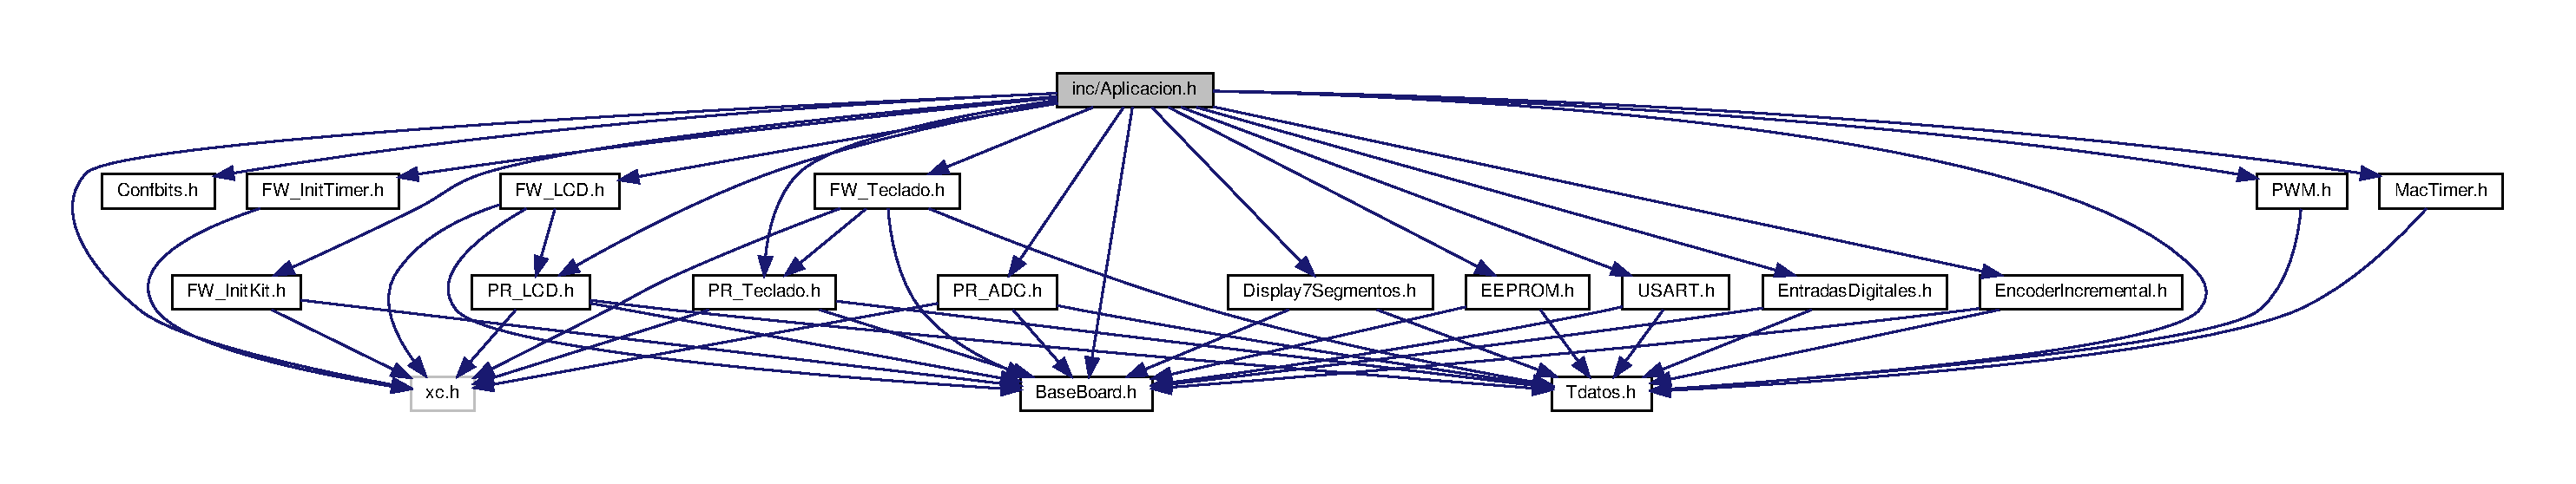
\includegraphics[width=350pt]{d3/dd0/Aplicacion_8h__incl}
\end{center}
\end{figure}
Gráfico de los archivos que directa o indirectamente incluyen a este archivo\+:\nopagebreak
\begin{figure}[H]
\begin{center}
\leavevmode
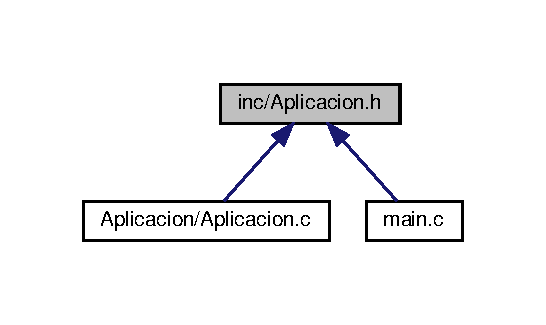
\includegraphics[width=262pt]{d9/d0c/Aplicacion_8h__dep__incl}
\end{center}
\end{figure}
\subsection*{Funciones}
\begin{DoxyCompactItemize}
\item 
void \hyperlink{Aplicacion_8h_a1c8d673b24659a71245bca4363fa1887}{Aplicacion} (void)
\begin{DoxyCompactList}\small\item\em Funcion principal. \end{DoxyCompactList}\end{DoxyCompactItemize}


\subsection{Documentación de las funciones}
\mbox{\Hypertarget{Aplicacion_8h_a1c8d673b24659a71245bca4363fa1887}\label{Aplicacion_8h_a1c8d673b24659a71245bca4363fa1887}} 
\index{Aplicacion.\+h@{Aplicacion.\+h}!Aplicacion@{Aplicacion}}
\index{Aplicacion@{Aplicacion}!Aplicacion.\+h@{Aplicacion.\+h}}
\subsubsection{\texorpdfstring{Aplicacion()}{Aplicacion()}}
{\footnotesize\ttfamily void Aplicacion (\begin{DoxyParamCaption}\item[{void}]{ }\end{DoxyParamCaption})}



Funcion principal. 

\begin{DoxyAuthor}{Autor}
Nicolas Ferragamo \href{mailto:nferragamo@est.frba.utn.edu.ar}{\tt nferragamo@est.\+frba.\+utn.\+edu.\+ar} 
\end{DoxyAuthor}
\begin{DoxyDate}{Fecha}
13 de junio del 2019 
\end{DoxyDate}


Definición en la línea 84 del archivo Aplicacion.\+c.

Gráfico de llamadas a esta función\+:\nopagebreak
\begin{figure}[H]
\begin{center}
\leavevmode
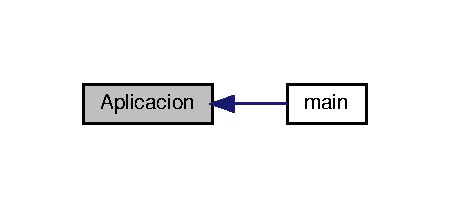
\includegraphics[width=216pt]{d4/da4/Aplicacion_8h_a1c8d673b24659a71245bca4363fa1887_icgraph}
\end{center}
\end{figure}

\hypertarget{BaseBoard_8h}{}\section{Referencia del Archivo inc/\+Base\+Board.h}
\label{BaseBoard_8h}\index{inc/\+Base\+Board.\+h@{inc/\+Base\+Board.\+h}}
Gráfico de los archivos que directa o indirectamente incluyen a este archivo\+:\nopagebreak
\begin{figure}[H]
\begin{center}
\leavevmode
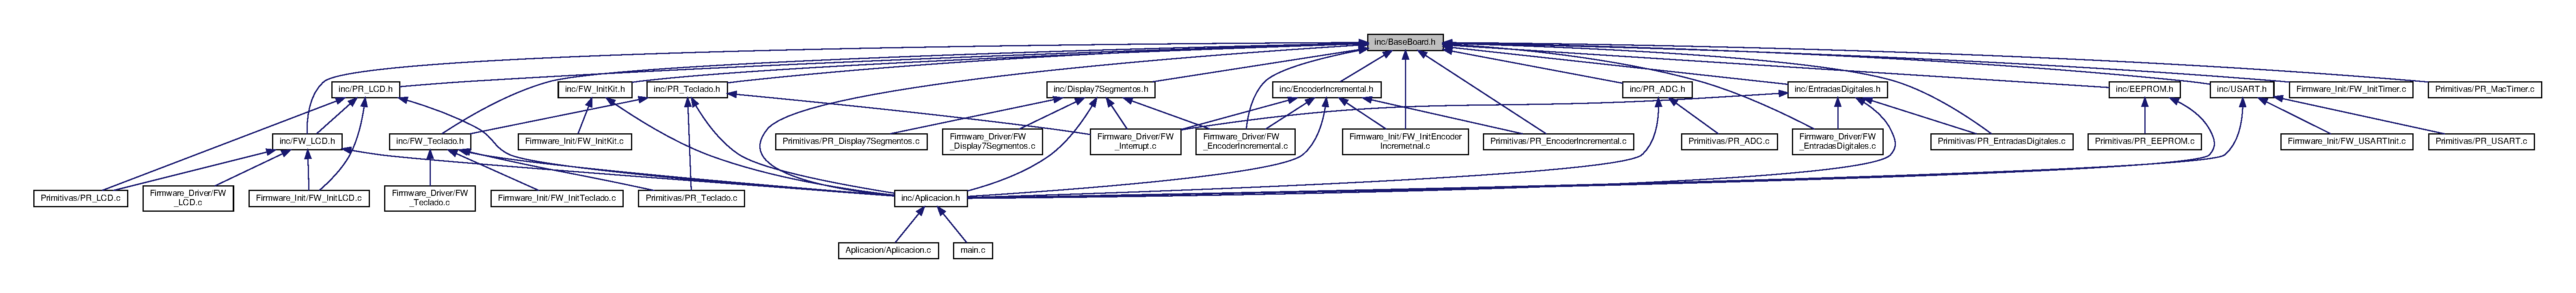
\includegraphics[width=350pt]{de/df5/BaseBoard_8h__dep__incl}
\end{center}
\end{figure}
\subsection*{defines}
\begin{DoxyCompactItemize}
\item 
\#define \hyperlink{BaseBoard_8h_abac3f33da608d244839fb370344cb585}{\+\_\+\+\_\+\+S\+H\+I\+E\+L\+D1}~1
\begin{DoxyCompactList}\small\item\em Selecciono el shield 1. \end{DoxyCompactList}\item 
\#define \hyperlink{BaseBoard_8h_a0a420bf23a04e7bb3d94dd685de69f73}{\+\_\+\+\_\+\+S\+H\+I\+E\+L\+D2}~2
\begin{DoxyCompactList}\small\item\em Selecciono el shield 2. \end{DoxyCompactList}\item 
\#define \hyperlink{BaseBoard_8h_a2af18bca5c2ed6af36e242305f94117d}{S\+H\+I\+E\+L\+D\+\_\+\+A\+C\+T\+I\+VO}~\hyperlink{BaseBoard_8h_abac3f33da608d244839fb370344cb585}{\+\_\+\+\_\+\+S\+H\+I\+E\+L\+D1}
\begin{DoxyCompactList}\small\item\em seleciona el shield activo \end{DoxyCompactList}\item 
\#define \hyperlink{BaseBoard_8h_aefae505e2588183f1921a9e840b16044}{L\+E\+D5}~L\+A\+T\+Dbits.\+L\+D0
\begin{DoxyCompactList}\small\item\em Indica ingreso a modo Boot\+Loader, puede ser usado por el usuario. \end{DoxyCompactList}\item 
\#define \hyperlink{BaseBoard_8h_ab922b15d42b90025c9e13c087d86ce81}{L\+E\+D6}~L\+A\+T\+Dbits.\+L\+D1
\begin{DoxyCompactList}\small\item\em Inica modo conectado, puede ser usado por el usuario. \end{DoxyCompactList}\item 
\#define \hyperlink{BaseBoard_8h_a8aa85ae9867fabf70ec72cd3bf6fb6b9}{L\+E\+D1}~L\+A\+T\+Dbits.\+L\+D2
\item 
\#define \hyperlink{BaseBoard_8h_ad09fe5bf321b9a2de26bd5e5b9af6424}{L\+E\+D2}~L\+A\+T\+Dbits.\+L\+D3
\item 
\#define \hyperlink{BaseBoard_8h_a4b7ff8e253a7412f83deba3a447028a8}{L\+E\+D3}~L\+A\+T\+Cbits.\+L\+C6
\item 
\#define \hyperlink{BaseBoard_8h_ae048837f20072bed467332b1bd1da9fa}{L\+E\+D4}~L\+A\+T\+Cbits.\+L\+C7
\item 
\#define \hyperlink{BaseBoard_8h_a514fed6fb5235478075a85e1a50b2aa7}{B\+O\+T1}~P\+O\+R\+T\+Dbits.\+R\+D4
\item 
\#define \hyperlink{BaseBoard_8h_a9de2fc6886584e508307bc2e6a5ab6d6}{B\+O\+T2}~P\+O\+R\+T\+Dbits.\+R\+D5
\item 
\#define \hyperlink{BaseBoard_8h_a145570f189e6e1523bf1dec991f477e7}{B\+O\+T3}~P\+O\+R\+T\+Dbits.\+R\+D6
\item 
\#define \hyperlink{BaseBoard_8h_ac54405c71508dad19a53e9c85c1462ef}{B\+O\+T4}~P\+O\+R\+T\+Dbits.\+R\+D7
\item 
\#define \hyperlink{BaseBoard_8h_a51ed185096fb63d11fe581879d4dd724}{D\+I\+S\+P1}~L\+A\+T\+Abits.\+L\+A4
\item 
\#define \hyperlink{BaseBoard_8h_abfd463b3ac57b2cc718abf1e9f07ee9c}{D\+I\+S\+P2}~L\+A\+T\+Abits.\+L\+A5
\item 
\#define \hyperlink{BaseBoard_8h_a6d6e11b0c9cc074a2c9af1747e68ef74}{D\+I\+S\+P3}~L\+A\+T\+Ebits.\+L\+E0
\item 
\#define \hyperlink{BaseBoard_8h_ad0225737fa73024abb640898eed601df}{D\+I\+S\+P4}~L\+A\+T\+Ebits.\+L\+E1
\item 
\#define \hyperlink{BaseBoard_8h_a8a5043e7ab655e37e903ffbd8b95d6b2}{D\+OT}~L\+A\+T\+Ebits.\+L\+E2
\item 
\#define \hyperlink{BaseBoard_8h_ac9067847b65e4676b029fc32cc0712cf}{Init\+\_\+\+Kit\+\_\+\+P\+U\+L\+S\+A\+D\+O\+R\+ES}~(P\+O\+R\+TD$^\wedge$0x\+F0)\&0x\+F0
\begin{DoxyCompactList}\small\item\em Nibble superior del puerto D. \end{DoxyCompactList}\item 
\#define \hyperlink{BaseBoard_8h_a2267fe6b19995924d44cef4b7d895535}{E\+N\+T\+R\+A\+DA}~1
\item 
\#define \hyperlink{BaseBoard_8h_a180bb04c74aa394e9c1eab5d26506c2b}{S\+A\+L\+I\+DA}~0
\item 
\#define \hyperlink{BaseBoard_8h_ad76d1750a6cdeebd506bfcd6752554d2}{ON}~1
\item 
\#define \hyperlink{BaseBoard_8h_a29e413f6725b2ba32d165ffaa35b01e5}{O\+FF}~0
\item 
\#define \hyperlink{BaseBoard_8h_af1d93aa494b8be71b3f8b3009d8fe032}{A\+C\+T\+I\+V\+O\+\_\+\+A\+L\+TO}~1
\item 
\#define \hyperlink{BaseBoard_8h_ae4b3d745479c62c04ea571e5feac8322}{A\+C\+T\+I\+V\+O\+\_\+\+B\+A\+JO}~0
\end{DoxyCompactItemize}


\subsection{Documentación de los \textquotesingle{}defines\textquotesingle{}}
\mbox{\Hypertarget{BaseBoard_8h_abac3f33da608d244839fb370344cb585}\label{BaseBoard_8h_abac3f33da608d244839fb370344cb585}} 
\index{Base\+Board.\+h@{Base\+Board.\+h}!\+\_\+\+\_\+\+S\+H\+I\+E\+L\+D1@{\+\_\+\+\_\+\+S\+H\+I\+E\+L\+D1}}
\index{\+\_\+\+\_\+\+S\+H\+I\+E\+L\+D1@{\+\_\+\+\_\+\+S\+H\+I\+E\+L\+D1}!Base\+Board.\+h@{Base\+Board.\+h}}
\subsubsection{\texorpdfstring{\+\_\+\+\_\+\+S\+H\+I\+E\+L\+D1}{\_\_SHIELD1}}
{\footnotesize\ttfamily \#define \+\_\+\+\_\+\+S\+H\+I\+E\+L\+D1~1}



Selecciono el shield 1. 



Definición en la línea 49 del archivo Base\+Board.\+h.

\mbox{\Hypertarget{BaseBoard_8h_a0a420bf23a04e7bb3d94dd685de69f73}\label{BaseBoard_8h_a0a420bf23a04e7bb3d94dd685de69f73}} 
\index{Base\+Board.\+h@{Base\+Board.\+h}!\+\_\+\+\_\+\+S\+H\+I\+E\+L\+D2@{\+\_\+\+\_\+\+S\+H\+I\+E\+L\+D2}}
\index{\+\_\+\+\_\+\+S\+H\+I\+E\+L\+D2@{\+\_\+\+\_\+\+S\+H\+I\+E\+L\+D2}!Base\+Board.\+h@{Base\+Board.\+h}}
\subsubsection{\texorpdfstring{\+\_\+\+\_\+\+S\+H\+I\+E\+L\+D2}{\_\_SHIELD2}}
{\footnotesize\ttfamily \#define \+\_\+\+\_\+\+S\+H\+I\+E\+L\+D2~2}



Selecciono el shield 2. 



Definición en la línea 50 del archivo Base\+Board.\+h.

\mbox{\Hypertarget{BaseBoard_8h_af1d93aa494b8be71b3f8b3009d8fe032}\label{BaseBoard_8h_af1d93aa494b8be71b3f8b3009d8fe032}} 
\index{Base\+Board.\+h@{Base\+Board.\+h}!A\+C\+T\+I\+V\+O\+\_\+\+A\+L\+TO@{A\+C\+T\+I\+V\+O\+\_\+\+A\+L\+TO}}
\index{A\+C\+T\+I\+V\+O\+\_\+\+A\+L\+TO@{A\+C\+T\+I\+V\+O\+\_\+\+A\+L\+TO}!Base\+Board.\+h@{Base\+Board.\+h}}
\subsubsection{\texorpdfstring{A\+C\+T\+I\+V\+O\+\_\+\+A\+L\+TO}{ACTIVO\_ALTO}}
{\footnotesize\ttfamily \#define A\+C\+T\+I\+V\+O\+\_\+\+A\+L\+TO~1}



Definición en la línea 135 del archivo Base\+Board.\+h.

\mbox{\Hypertarget{BaseBoard_8h_ae4b3d745479c62c04ea571e5feac8322}\label{BaseBoard_8h_ae4b3d745479c62c04ea571e5feac8322}} 
\index{Base\+Board.\+h@{Base\+Board.\+h}!A\+C\+T\+I\+V\+O\+\_\+\+B\+A\+JO@{A\+C\+T\+I\+V\+O\+\_\+\+B\+A\+JO}}
\index{A\+C\+T\+I\+V\+O\+\_\+\+B\+A\+JO@{A\+C\+T\+I\+V\+O\+\_\+\+B\+A\+JO}!Base\+Board.\+h@{Base\+Board.\+h}}
\subsubsection{\texorpdfstring{A\+C\+T\+I\+V\+O\+\_\+\+B\+A\+JO}{ACTIVO\_BAJO}}
{\footnotesize\ttfamily \#define A\+C\+T\+I\+V\+O\+\_\+\+B\+A\+JO~0}



Definición en la línea 136 del archivo Base\+Board.\+h.

\mbox{\Hypertarget{BaseBoard_8h_a514fed6fb5235478075a85e1a50b2aa7}\label{BaseBoard_8h_a514fed6fb5235478075a85e1a50b2aa7}} 
\index{Base\+Board.\+h@{Base\+Board.\+h}!B\+O\+T1@{B\+O\+T1}}
\index{B\+O\+T1@{B\+O\+T1}!Base\+Board.\+h@{Base\+Board.\+h}}
\subsubsection{\texorpdfstring{B\+O\+T1}{BOT1}}
{\footnotesize\ttfamily \#define B\+O\+T1~P\+O\+R\+T\+Dbits.\+R\+D4}



Definición en la línea 64 del archivo Base\+Board.\+h.

\mbox{\Hypertarget{BaseBoard_8h_a9de2fc6886584e508307bc2e6a5ab6d6}\label{BaseBoard_8h_a9de2fc6886584e508307bc2e6a5ab6d6}} 
\index{Base\+Board.\+h@{Base\+Board.\+h}!B\+O\+T2@{B\+O\+T2}}
\index{B\+O\+T2@{B\+O\+T2}!Base\+Board.\+h@{Base\+Board.\+h}}
\subsubsection{\texorpdfstring{B\+O\+T2}{BOT2}}
{\footnotesize\ttfamily \#define B\+O\+T2~P\+O\+R\+T\+Dbits.\+R\+D5}



Definición en la línea 65 del archivo Base\+Board.\+h.

\mbox{\Hypertarget{BaseBoard_8h_a145570f189e6e1523bf1dec991f477e7}\label{BaseBoard_8h_a145570f189e6e1523bf1dec991f477e7}} 
\index{Base\+Board.\+h@{Base\+Board.\+h}!B\+O\+T3@{B\+O\+T3}}
\index{B\+O\+T3@{B\+O\+T3}!Base\+Board.\+h@{Base\+Board.\+h}}
\subsubsection{\texorpdfstring{B\+O\+T3}{BOT3}}
{\footnotesize\ttfamily \#define B\+O\+T3~P\+O\+R\+T\+Dbits.\+R\+D6}



Definición en la línea 66 del archivo Base\+Board.\+h.

\mbox{\Hypertarget{BaseBoard_8h_ac54405c71508dad19a53e9c85c1462ef}\label{BaseBoard_8h_ac54405c71508dad19a53e9c85c1462ef}} 
\index{Base\+Board.\+h@{Base\+Board.\+h}!B\+O\+T4@{B\+O\+T4}}
\index{B\+O\+T4@{B\+O\+T4}!Base\+Board.\+h@{Base\+Board.\+h}}
\subsubsection{\texorpdfstring{B\+O\+T4}{BOT4}}
{\footnotesize\ttfamily \#define B\+O\+T4~P\+O\+R\+T\+Dbits.\+R\+D7}



Definición en la línea 67 del archivo Base\+Board.\+h.

\mbox{\Hypertarget{BaseBoard_8h_a51ed185096fb63d11fe581879d4dd724}\label{BaseBoard_8h_a51ed185096fb63d11fe581879d4dd724}} 
\index{Base\+Board.\+h@{Base\+Board.\+h}!D\+I\+S\+P1@{D\+I\+S\+P1}}
\index{D\+I\+S\+P1@{D\+I\+S\+P1}!Base\+Board.\+h@{Base\+Board.\+h}}
\subsubsection{\texorpdfstring{D\+I\+S\+P1}{DISP1}}
{\footnotesize\ttfamily \#define D\+I\+S\+P1~L\+A\+T\+Abits.\+L\+A4}



Definición en la línea 70 del archivo Base\+Board.\+h.

\mbox{\Hypertarget{BaseBoard_8h_abfd463b3ac57b2cc718abf1e9f07ee9c}\label{BaseBoard_8h_abfd463b3ac57b2cc718abf1e9f07ee9c}} 
\index{Base\+Board.\+h@{Base\+Board.\+h}!D\+I\+S\+P2@{D\+I\+S\+P2}}
\index{D\+I\+S\+P2@{D\+I\+S\+P2}!Base\+Board.\+h@{Base\+Board.\+h}}
\subsubsection{\texorpdfstring{D\+I\+S\+P2}{DISP2}}
{\footnotesize\ttfamily \#define D\+I\+S\+P2~L\+A\+T\+Abits.\+L\+A5}



Definición en la línea 71 del archivo Base\+Board.\+h.

\mbox{\Hypertarget{BaseBoard_8h_a6d6e11b0c9cc074a2c9af1747e68ef74}\label{BaseBoard_8h_a6d6e11b0c9cc074a2c9af1747e68ef74}} 
\index{Base\+Board.\+h@{Base\+Board.\+h}!D\+I\+S\+P3@{D\+I\+S\+P3}}
\index{D\+I\+S\+P3@{D\+I\+S\+P3}!Base\+Board.\+h@{Base\+Board.\+h}}
\subsubsection{\texorpdfstring{D\+I\+S\+P3}{DISP3}}
{\footnotesize\ttfamily \#define D\+I\+S\+P3~L\+A\+T\+Ebits.\+L\+E0}



Definición en la línea 72 del archivo Base\+Board.\+h.

\mbox{\Hypertarget{BaseBoard_8h_ad0225737fa73024abb640898eed601df}\label{BaseBoard_8h_ad0225737fa73024abb640898eed601df}} 
\index{Base\+Board.\+h@{Base\+Board.\+h}!D\+I\+S\+P4@{D\+I\+S\+P4}}
\index{D\+I\+S\+P4@{D\+I\+S\+P4}!Base\+Board.\+h@{Base\+Board.\+h}}
\subsubsection{\texorpdfstring{D\+I\+S\+P4}{DISP4}}
{\footnotesize\ttfamily \#define D\+I\+S\+P4~L\+A\+T\+Ebits.\+L\+E1}



Definición en la línea 73 del archivo Base\+Board.\+h.

\mbox{\Hypertarget{BaseBoard_8h_a8a5043e7ab655e37e903ffbd8b95d6b2}\label{BaseBoard_8h_a8a5043e7ab655e37e903ffbd8b95d6b2}} 
\index{Base\+Board.\+h@{Base\+Board.\+h}!D\+OT@{D\+OT}}
\index{D\+OT@{D\+OT}!Base\+Board.\+h@{Base\+Board.\+h}}
\subsubsection{\texorpdfstring{D\+OT}{DOT}}
{\footnotesize\ttfamily \#define D\+OT~L\+A\+T\+Ebits.\+L\+E2}



Definición en la línea 74 del archivo Base\+Board.\+h.

\mbox{\Hypertarget{BaseBoard_8h_a2267fe6b19995924d44cef4b7d895535}\label{BaseBoard_8h_a2267fe6b19995924d44cef4b7d895535}} 
\index{Base\+Board.\+h@{Base\+Board.\+h}!E\+N\+T\+R\+A\+DA@{E\+N\+T\+R\+A\+DA}}
\index{E\+N\+T\+R\+A\+DA@{E\+N\+T\+R\+A\+DA}!Base\+Board.\+h@{Base\+Board.\+h}}
\subsubsection{\texorpdfstring{E\+N\+T\+R\+A\+DA}{ENTRADA}}
{\footnotesize\ttfamily \#define E\+N\+T\+R\+A\+DA~1}



Definición en la línea 129 del archivo Base\+Board.\+h.

\mbox{\Hypertarget{BaseBoard_8h_ac9067847b65e4676b029fc32cc0712cf}\label{BaseBoard_8h_ac9067847b65e4676b029fc32cc0712cf}} 
\index{Base\+Board.\+h@{Base\+Board.\+h}!Init\+\_\+\+Kit\+\_\+\+P\+U\+L\+S\+A\+D\+O\+R\+ES@{Init\+\_\+\+Kit\+\_\+\+P\+U\+L\+S\+A\+D\+O\+R\+ES}}
\index{Init\+\_\+\+Kit\+\_\+\+P\+U\+L\+S\+A\+D\+O\+R\+ES@{Init\+\_\+\+Kit\+\_\+\+P\+U\+L\+S\+A\+D\+O\+R\+ES}!Base\+Board.\+h@{Base\+Board.\+h}}
\subsubsection{\texorpdfstring{Init\+\_\+\+Kit\+\_\+\+P\+U\+L\+S\+A\+D\+O\+R\+ES}{Init\_Kit\_PULSADORES}}
{\footnotesize\ttfamily \#define Init\+\_\+\+Kit\+\_\+\+P\+U\+L\+S\+A\+D\+O\+R\+ES~(P\+O\+R\+TD$^\wedge$0x\+F0)\&0x\+F0}



Nibble superior del puerto D. 



Definición en la línea 76 del archivo Base\+Board.\+h.

\mbox{\Hypertarget{BaseBoard_8h_a8aa85ae9867fabf70ec72cd3bf6fb6b9}\label{BaseBoard_8h_a8aa85ae9867fabf70ec72cd3bf6fb6b9}} 
\index{Base\+Board.\+h@{Base\+Board.\+h}!L\+E\+D1@{L\+E\+D1}}
\index{L\+E\+D1@{L\+E\+D1}!Base\+Board.\+h@{Base\+Board.\+h}}
\subsubsection{\texorpdfstring{L\+E\+D1}{LED1}}
{\footnotesize\ttfamily \#define L\+E\+D1~L\+A\+T\+Dbits.\+L\+D2}



Definición en la línea 58 del archivo Base\+Board.\+h.

\mbox{\Hypertarget{BaseBoard_8h_ad09fe5bf321b9a2de26bd5e5b9af6424}\label{BaseBoard_8h_ad09fe5bf321b9a2de26bd5e5b9af6424}} 
\index{Base\+Board.\+h@{Base\+Board.\+h}!L\+E\+D2@{L\+E\+D2}}
\index{L\+E\+D2@{L\+E\+D2}!Base\+Board.\+h@{Base\+Board.\+h}}
\subsubsection{\texorpdfstring{L\+E\+D2}{LED2}}
{\footnotesize\ttfamily \#define L\+E\+D2~L\+A\+T\+Dbits.\+L\+D3}



Definición en la línea 59 del archivo Base\+Board.\+h.

\mbox{\Hypertarget{BaseBoard_8h_a4b7ff8e253a7412f83deba3a447028a8}\label{BaseBoard_8h_a4b7ff8e253a7412f83deba3a447028a8}} 
\index{Base\+Board.\+h@{Base\+Board.\+h}!L\+E\+D3@{L\+E\+D3}}
\index{L\+E\+D3@{L\+E\+D3}!Base\+Board.\+h@{Base\+Board.\+h}}
\subsubsection{\texorpdfstring{L\+E\+D3}{LED3}}
{\footnotesize\ttfamily \#define L\+E\+D3~L\+A\+T\+Cbits.\+L\+C6}



Definición en la línea 60 del archivo Base\+Board.\+h.

\mbox{\Hypertarget{BaseBoard_8h_ae048837f20072bed467332b1bd1da9fa}\label{BaseBoard_8h_ae048837f20072bed467332b1bd1da9fa}} 
\index{Base\+Board.\+h@{Base\+Board.\+h}!L\+E\+D4@{L\+E\+D4}}
\index{L\+E\+D4@{L\+E\+D4}!Base\+Board.\+h@{Base\+Board.\+h}}
\subsubsection{\texorpdfstring{L\+E\+D4}{LED4}}
{\footnotesize\ttfamily \#define L\+E\+D4~L\+A\+T\+Cbits.\+L\+C7}



Definición en la línea 61 del archivo Base\+Board.\+h.

\mbox{\Hypertarget{BaseBoard_8h_aefae505e2588183f1921a9e840b16044}\label{BaseBoard_8h_aefae505e2588183f1921a9e840b16044}} 
\index{Base\+Board.\+h@{Base\+Board.\+h}!L\+E\+D5@{L\+E\+D5}}
\index{L\+E\+D5@{L\+E\+D5}!Base\+Board.\+h@{Base\+Board.\+h}}
\subsubsection{\texorpdfstring{L\+E\+D5}{LED5}}
{\footnotesize\ttfamily \#define L\+E\+D5~L\+A\+T\+Dbits.\+L\+D0}



Indica ingreso a modo Boot\+Loader, puede ser usado por el usuario. 



Definición en la línea 56 del archivo Base\+Board.\+h.

\mbox{\Hypertarget{BaseBoard_8h_ab922b15d42b90025c9e13c087d86ce81}\label{BaseBoard_8h_ab922b15d42b90025c9e13c087d86ce81}} 
\index{Base\+Board.\+h@{Base\+Board.\+h}!L\+E\+D6@{L\+E\+D6}}
\index{L\+E\+D6@{L\+E\+D6}!Base\+Board.\+h@{Base\+Board.\+h}}
\subsubsection{\texorpdfstring{L\+E\+D6}{LED6}}
{\footnotesize\ttfamily \#define L\+E\+D6~L\+A\+T\+Dbits.\+L\+D1}



Inica modo conectado, puede ser usado por el usuario. 



Definición en la línea 57 del archivo Base\+Board.\+h.

\mbox{\Hypertarget{BaseBoard_8h_a29e413f6725b2ba32d165ffaa35b01e5}\label{BaseBoard_8h_a29e413f6725b2ba32d165ffaa35b01e5}} 
\index{Base\+Board.\+h@{Base\+Board.\+h}!O\+FF@{O\+FF}}
\index{O\+FF@{O\+FF}!Base\+Board.\+h@{Base\+Board.\+h}}
\subsubsection{\texorpdfstring{O\+FF}{OFF}}
{\footnotesize\ttfamily \#define O\+FF~0}



Definición en la línea 133 del archivo Base\+Board.\+h.

\mbox{\Hypertarget{BaseBoard_8h_ad76d1750a6cdeebd506bfcd6752554d2}\label{BaseBoard_8h_ad76d1750a6cdeebd506bfcd6752554d2}} 
\index{Base\+Board.\+h@{Base\+Board.\+h}!ON@{ON}}
\index{ON@{ON}!Base\+Board.\+h@{Base\+Board.\+h}}
\subsubsection{\texorpdfstring{ON}{ON}}
{\footnotesize\ttfamily \#define ON~1}



Definición en la línea 132 del archivo Base\+Board.\+h.

\mbox{\Hypertarget{BaseBoard_8h_a180bb04c74aa394e9c1eab5d26506c2b}\label{BaseBoard_8h_a180bb04c74aa394e9c1eab5d26506c2b}} 
\index{Base\+Board.\+h@{Base\+Board.\+h}!S\+A\+L\+I\+DA@{S\+A\+L\+I\+DA}}
\index{S\+A\+L\+I\+DA@{S\+A\+L\+I\+DA}!Base\+Board.\+h@{Base\+Board.\+h}}
\subsubsection{\texorpdfstring{S\+A\+L\+I\+DA}{SALIDA}}
{\footnotesize\ttfamily \#define S\+A\+L\+I\+DA~0}



Definición en la línea 130 del archivo Base\+Board.\+h.

\mbox{\Hypertarget{BaseBoard_8h_a2af18bca5c2ed6af36e242305f94117d}\label{BaseBoard_8h_a2af18bca5c2ed6af36e242305f94117d}} 
\index{Base\+Board.\+h@{Base\+Board.\+h}!S\+H\+I\+E\+L\+D\+\_\+\+A\+C\+T\+I\+VO@{S\+H\+I\+E\+L\+D\+\_\+\+A\+C\+T\+I\+VO}}
\index{S\+H\+I\+E\+L\+D\+\_\+\+A\+C\+T\+I\+VO@{S\+H\+I\+E\+L\+D\+\_\+\+A\+C\+T\+I\+VO}!Base\+Board.\+h@{Base\+Board.\+h}}
\subsubsection{\texorpdfstring{S\+H\+I\+E\+L\+D\+\_\+\+A\+C\+T\+I\+VO}{SHIELD\_ACTIVO}}
{\footnotesize\ttfamily \#define S\+H\+I\+E\+L\+D\+\_\+\+A\+C\+T\+I\+VO~\hyperlink{BaseBoard_8h_abac3f33da608d244839fb370344cb585}{\+\_\+\+\_\+\+S\+H\+I\+E\+L\+D1}}



seleciona el shield activo 



Definición en la línea 51 del archivo Base\+Board.\+h.


\hypertarget{Confbits_8h}{}\section{Referencia del Archivo inc/\+Confbits.h}
\label{Confbits_8h}\index{inc/\+Confbits.\+h@{inc/\+Confbits.\+h}}
Gráfico de los archivos que directa o indirectamente incluyen a este archivo\+:\nopagebreak
\begin{figure}[H]
\begin{center}
\leavevmode
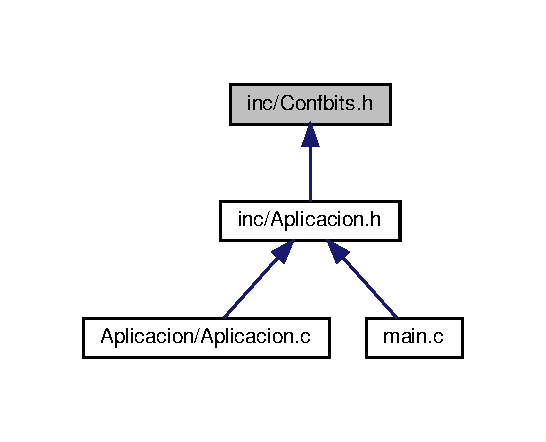
\includegraphics[width=262pt]{dc/d43/Confbits_8h__dep__incl}
\end{center}
\end{figure}
\subsection*{defines}
\begin{DoxyCompactItemize}
\item 
\#define \hyperlink{Confbits_8h_a3d24a8ac8f673b60ac35b6d92fe72747}{X\+T\+A\+L\+\_\+\+F\+R\+EQ}~20000000
\end{DoxyCompactItemize}


\subsection{Documentación de los \textquotesingle{}defines\textquotesingle{}}
\mbox{\Hypertarget{Confbits_8h_a3d24a8ac8f673b60ac35b6d92fe72747}\label{Confbits_8h_a3d24a8ac8f673b60ac35b6d92fe72747}} 
\index{Confbits.\+h@{Confbits.\+h}!X\+T\+A\+L\+\_\+\+F\+R\+EQ@{X\+T\+A\+L\+\_\+\+F\+R\+EQ}}
\index{X\+T\+A\+L\+\_\+\+F\+R\+EQ@{X\+T\+A\+L\+\_\+\+F\+R\+EQ}!Confbits.\+h@{Confbits.\+h}}
\subsubsection{\texorpdfstring{X\+T\+A\+L\+\_\+\+F\+R\+EQ}{XTAL\_FREQ}}
{\footnotesize\ttfamily \#define X\+T\+A\+L\+\_\+\+F\+R\+EQ~20000000}



Definición en la línea 27 del archivo Confbits.\+h.


\hypertarget{Display7Segmentos_8h}{}\section{Referencia del Archivo inc/\+Display7\+Segmentos.h}
\label{Display7Segmentos_8h}\index{inc/\+Display7\+Segmentos.\+h@{inc/\+Display7\+Segmentos.\+h}}
{\ttfamily \#include \char`\"{}Tdatos.\+h\char`\"{}}\newline
{\ttfamily \#include \char`\"{}Base\+Board.\+h\char`\"{}}\newline
Dependencia gráfica adjunta para Display7\+Segmentos.\+h\+:\nopagebreak
\begin{figure}[H]
\begin{center}
\leavevmode
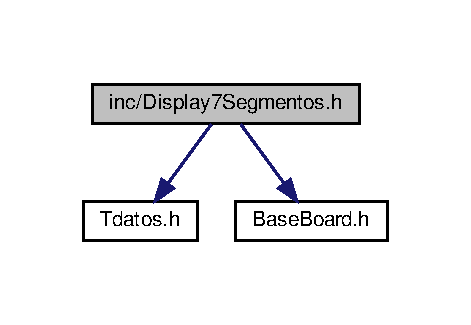
\includegraphics[width=226pt]{d4/d1d/Display7Segmentos_8h__incl}
\end{center}
\end{figure}
Gráfico de los archivos que directa o indirectamente incluyen a este archivo\+:\nopagebreak
\begin{figure}[H]
\begin{center}
\leavevmode
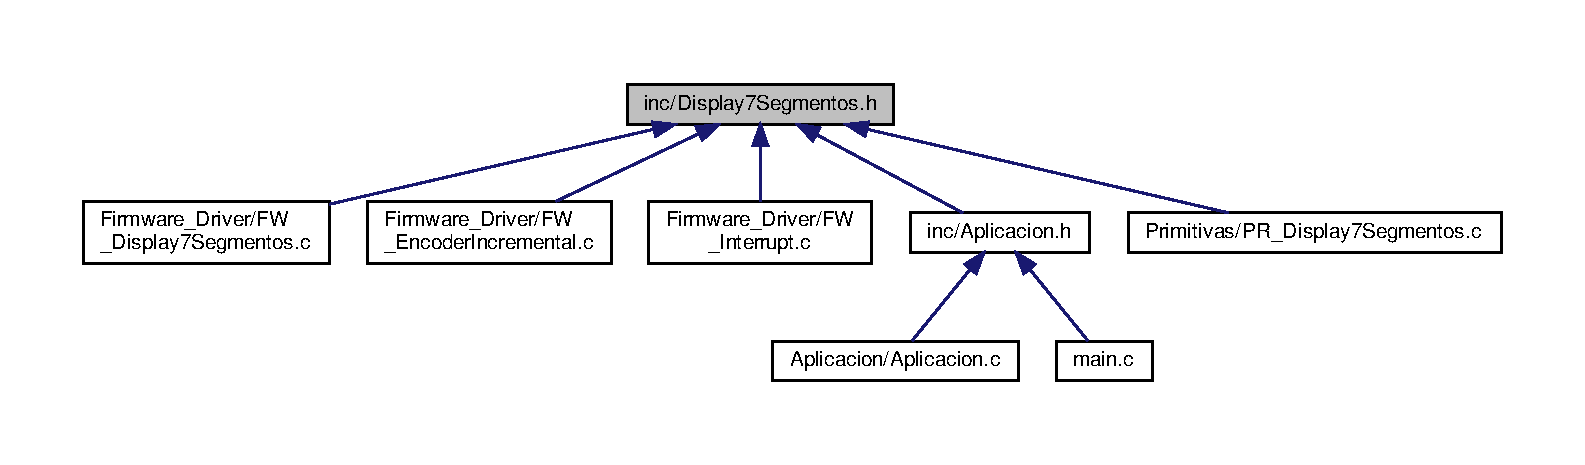
\includegraphics[width=350pt]{d5/d86/Display7Segmentos_8h__dep__incl}
\end{center}
\end{figure}
\subsection*{defines}
\begin{DoxyCompactItemize}
\item 
\#define \hyperlink{Display7Segmentos_8h_a4a6bdb32c7783dae55095173319d52ab}{D\+P\+\_\+\+D\+I\+G\+I\+T\+OS}~4
\begin{DoxyCompactList}\small\item\em N�meros de diplays. \end{DoxyCompactList}\item 
\#define \hyperlink{Display7Segmentos_8h_a664b6ba4767ee385ae6010587d9d8b9a}{D\+P\+\_\+\+T\+IC}~5
\begin{DoxyCompactList}\small\item\em Demora del barrido. \end{DoxyCompactList}\item 
\#define \hyperlink{Display7Segmentos_8h_a047430db55a3f99e1193bcb38509fbf4}{D\+P\+\_\+\+D\+I\+S\+P4}~L\+A\+T\+Abits.\+L\+A4
\item 
\#define \hyperlink{Display7Segmentos_8h_a10fe6f48e47a03df39d4485c3c338f4f}{D\+P\+\_\+\+D\+I\+S\+P3}~L\+A\+T\+Abits.\+L\+A5
\item 
\#define \hyperlink{Display7Segmentos_8h_a6c15794d391d0969d6ad81a6a3a59679}{D\+P\+\_\+\+D\+I\+S\+P2}~L\+A\+T\+Ebits.\+L\+E0
\item 
\#define \hyperlink{Display7Segmentos_8h_a2eb7c4c009ccf0afa44b5267a4eae3e7}{D\+P\+\_\+\+D\+I\+S\+P1}~L\+A\+T\+Ebits.\+L\+E1
\item 
\#define \hyperlink{Display7Segmentos_8h_a5ca40760822b7225232a2438151c9e7e}{D\+P\+\_\+\+S\+E\+G\+M\+E\+N\+T\+OA}~L\+A\+T\+Abits.\+L\+A0
\item 
\#define \hyperlink{Display7Segmentos_8h_a65759c7793e1b2b1525f288fcff151e3}{D\+P\+\_\+\+S\+E\+G\+M\+E\+N\+T\+OB}~L\+A\+T\+Abits.\+L\+A1
\item 
\#define \hyperlink{Display7Segmentos_8h_a18204a3cce46b4034c80eb413bb78ef0}{D\+P\+\_\+\+S\+E\+G\+M\+E\+N\+T\+OC}~L\+A\+T\+Abits.\+L\+A2
\item 
\#define \hyperlink{Display7Segmentos_8h_a83b47fac44e744fe583978dfb4d4a85a}{D\+P\+\_\+\+S\+E\+G\+M\+E\+N\+T\+OD}~L\+A\+T\+Abits.\+L\+A3
\item 
\#define \hyperlink{Display7Segmentos_8h_a5906f15756de8f01bc57c1f8803d013f}{D\+P\+\_\+\+D\+OT}~L\+A\+T\+Ebits.\+L\+E2
\end{DoxyCompactItemize}
\subsection*{Funciones}
\begin{DoxyCompactItemize}
\item 
void \hyperlink{Display7Segmentos_8h_a41b93045d294c7b52da4d1aa857383dd}{D\+P\+\_\+\+Barrido\+Display} (void)
\begin{DoxyCompactList}\small\item\em Realiza el barrido de los displays. \end{DoxyCompactList}\item 
void \hyperlink{Display7Segmentos_8h_ad93a0dc9bed0921da3a840880464fdc4}{D\+P\+\_\+\+Display\+B\+CD} (\hyperlink{Tdatos_8h_adf4d876453337156dde61095e1f20223}{uint16\+\_\+t} valor, \hyperlink{Tdatos_8h_aba7bc1797add20fe3efdf37ced1182c5}{uint8\+\_\+t} dsp)
\item 
void \hyperlink{Display7Segmentos_8h_a372f00db9001b490f7cec5e8d86b559b}{D\+P\+\_\+\+Tic} (void)
\begin{DoxyCompactList}\small\item\em Se encarga de la demora del barrido. \end{DoxyCompactList}\end{DoxyCompactItemize}
\subsection*{Variables}
\begin{DoxyCompactItemize}
\item 
volatile \hyperlink{Tdatos_8h_aba7bc1797add20fe3efdf37ced1182c5}{uint8\+\_\+t} \hyperlink{Display7Segmentos_8h_ad2a45360f8387fbe8e885bb9f3114ea5}{D\+P\+\_\+msg\+Display} \mbox{[}\hyperlink{Display7Segmentos_8h_a4a6bdb32c7783dae55095173319d52ab}{D\+P\+\_\+\+D\+I\+G\+I\+T\+OS}\mbox{]}
\item 
volatile \hyperlink{Tdatos_8h_aba7bc1797add20fe3efdf37ced1182c5}{uint8\+\_\+t} \hyperlink{Display7Segmentos_8h_a65e480a33e370b81cef253cb71d2a22b}{D\+P\+\_\+\+Delay}
\end{DoxyCompactItemize}


\subsection{Documentación de los \textquotesingle{}defines\textquotesingle{}}
\mbox{\Hypertarget{Display7Segmentos_8h_a4a6bdb32c7783dae55095173319d52ab}\label{Display7Segmentos_8h_a4a6bdb32c7783dae55095173319d52ab}} 
\index{Display7\+Segmentos.\+h@{Display7\+Segmentos.\+h}!D\+P\+\_\+\+D\+I\+G\+I\+T\+OS@{D\+P\+\_\+\+D\+I\+G\+I\+T\+OS}}
\index{D\+P\+\_\+\+D\+I\+G\+I\+T\+OS@{D\+P\+\_\+\+D\+I\+G\+I\+T\+OS}!Display7\+Segmentos.\+h@{Display7\+Segmentos.\+h}}
\subsubsection{\texorpdfstring{D\+P\+\_\+\+D\+I\+G\+I\+T\+OS}{DP\_DIGITOS}}
{\footnotesize\ttfamily \#define D\+P\+\_\+\+D\+I\+G\+I\+T\+OS~4}



N�meros de diplays. 



Definición en la línea 49 del archivo Display7\+Segmentos.\+h.

\mbox{\Hypertarget{Display7Segmentos_8h_a2eb7c4c009ccf0afa44b5267a4eae3e7}\label{Display7Segmentos_8h_a2eb7c4c009ccf0afa44b5267a4eae3e7}} 
\index{Display7\+Segmentos.\+h@{Display7\+Segmentos.\+h}!D\+P\+\_\+\+D\+I\+S\+P1@{D\+P\+\_\+\+D\+I\+S\+P1}}
\index{D\+P\+\_\+\+D\+I\+S\+P1@{D\+P\+\_\+\+D\+I\+S\+P1}!Display7\+Segmentos.\+h@{Display7\+Segmentos.\+h}}
\subsubsection{\texorpdfstring{D\+P\+\_\+\+D\+I\+S\+P1}{DP\_DISP1}}
{\footnotesize\ttfamily \#define D\+P\+\_\+\+D\+I\+S\+P1~L\+A\+T\+Ebits.\+L\+E1}



Definición en la línea 55 del archivo Display7\+Segmentos.\+h.

\mbox{\Hypertarget{Display7Segmentos_8h_a6c15794d391d0969d6ad81a6a3a59679}\label{Display7Segmentos_8h_a6c15794d391d0969d6ad81a6a3a59679}} 
\index{Display7\+Segmentos.\+h@{Display7\+Segmentos.\+h}!D\+P\+\_\+\+D\+I\+S\+P2@{D\+P\+\_\+\+D\+I\+S\+P2}}
\index{D\+P\+\_\+\+D\+I\+S\+P2@{D\+P\+\_\+\+D\+I\+S\+P2}!Display7\+Segmentos.\+h@{Display7\+Segmentos.\+h}}
\subsubsection{\texorpdfstring{D\+P\+\_\+\+D\+I\+S\+P2}{DP\_DISP2}}
{\footnotesize\ttfamily \#define D\+P\+\_\+\+D\+I\+S\+P2~L\+A\+T\+Ebits.\+L\+E0}



Definición en la línea 54 del archivo Display7\+Segmentos.\+h.

\mbox{\Hypertarget{Display7Segmentos_8h_a10fe6f48e47a03df39d4485c3c338f4f}\label{Display7Segmentos_8h_a10fe6f48e47a03df39d4485c3c338f4f}} 
\index{Display7\+Segmentos.\+h@{Display7\+Segmentos.\+h}!D\+P\+\_\+\+D\+I\+S\+P3@{D\+P\+\_\+\+D\+I\+S\+P3}}
\index{D\+P\+\_\+\+D\+I\+S\+P3@{D\+P\+\_\+\+D\+I\+S\+P3}!Display7\+Segmentos.\+h@{Display7\+Segmentos.\+h}}
\subsubsection{\texorpdfstring{D\+P\+\_\+\+D\+I\+S\+P3}{DP\_DISP3}}
{\footnotesize\ttfamily \#define D\+P\+\_\+\+D\+I\+S\+P3~L\+A\+T\+Abits.\+L\+A5}



Definición en la línea 53 del archivo Display7\+Segmentos.\+h.

\mbox{\Hypertarget{Display7Segmentos_8h_a047430db55a3f99e1193bcb38509fbf4}\label{Display7Segmentos_8h_a047430db55a3f99e1193bcb38509fbf4}} 
\index{Display7\+Segmentos.\+h@{Display7\+Segmentos.\+h}!D\+P\+\_\+\+D\+I\+S\+P4@{D\+P\+\_\+\+D\+I\+S\+P4}}
\index{D\+P\+\_\+\+D\+I\+S\+P4@{D\+P\+\_\+\+D\+I\+S\+P4}!Display7\+Segmentos.\+h@{Display7\+Segmentos.\+h}}
\subsubsection{\texorpdfstring{D\+P\+\_\+\+D\+I\+S\+P4}{DP\_DISP4}}
{\footnotesize\ttfamily \#define D\+P\+\_\+\+D\+I\+S\+P4~L\+A\+T\+Abits.\+L\+A4}



Definición en la línea 52 del archivo Display7\+Segmentos.\+h.

\mbox{\Hypertarget{Display7Segmentos_8h_a5906f15756de8f01bc57c1f8803d013f}\label{Display7Segmentos_8h_a5906f15756de8f01bc57c1f8803d013f}} 
\index{Display7\+Segmentos.\+h@{Display7\+Segmentos.\+h}!D\+P\+\_\+\+D\+OT@{D\+P\+\_\+\+D\+OT}}
\index{D\+P\+\_\+\+D\+OT@{D\+P\+\_\+\+D\+OT}!Display7\+Segmentos.\+h@{Display7\+Segmentos.\+h}}
\subsubsection{\texorpdfstring{D\+P\+\_\+\+D\+OT}{DP\_DOT}}
{\footnotesize\ttfamily \#define D\+P\+\_\+\+D\+OT~L\+A\+T\+Ebits.\+L\+E2}



Definición en la línea 62 del archivo Display7\+Segmentos.\+h.

\mbox{\Hypertarget{Display7Segmentos_8h_a5ca40760822b7225232a2438151c9e7e}\label{Display7Segmentos_8h_a5ca40760822b7225232a2438151c9e7e}} 
\index{Display7\+Segmentos.\+h@{Display7\+Segmentos.\+h}!D\+P\+\_\+\+S\+E\+G\+M\+E\+N\+T\+OA@{D\+P\+\_\+\+S\+E\+G\+M\+E\+N\+T\+OA}}
\index{D\+P\+\_\+\+S\+E\+G\+M\+E\+N\+T\+OA@{D\+P\+\_\+\+S\+E\+G\+M\+E\+N\+T\+OA}!Display7\+Segmentos.\+h@{Display7\+Segmentos.\+h}}
\subsubsection{\texorpdfstring{D\+P\+\_\+\+S\+E\+G\+M\+E\+N\+T\+OA}{DP\_SEGMENTOA}}
{\footnotesize\ttfamily \#define D\+P\+\_\+\+S\+E\+G\+M\+E\+N\+T\+OA~L\+A\+T\+Abits.\+L\+A0}



Definición en la línea 58 del archivo Display7\+Segmentos.\+h.

\mbox{\Hypertarget{Display7Segmentos_8h_a65759c7793e1b2b1525f288fcff151e3}\label{Display7Segmentos_8h_a65759c7793e1b2b1525f288fcff151e3}} 
\index{Display7\+Segmentos.\+h@{Display7\+Segmentos.\+h}!D\+P\+\_\+\+S\+E\+G\+M\+E\+N\+T\+OB@{D\+P\+\_\+\+S\+E\+G\+M\+E\+N\+T\+OB}}
\index{D\+P\+\_\+\+S\+E\+G\+M\+E\+N\+T\+OB@{D\+P\+\_\+\+S\+E\+G\+M\+E\+N\+T\+OB}!Display7\+Segmentos.\+h@{Display7\+Segmentos.\+h}}
\subsubsection{\texorpdfstring{D\+P\+\_\+\+S\+E\+G\+M\+E\+N\+T\+OB}{DP\_SEGMENTOB}}
{\footnotesize\ttfamily \#define D\+P\+\_\+\+S\+E\+G\+M\+E\+N\+T\+OB~L\+A\+T\+Abits.\+L\+A1}



Definición en la línea 59 del archivo Display7\+Segmentos.\+h.

\mbox{\Hypertarget{Display7Segmentos_8h_a18204a3cce46b4034c80eb413bb78ef0}\label{Display7Segmentos_8h_a18204a3cce46b4034c80eb413bb78ef0}} 
\index{Display7\+Segmentos.\+h@{Display7\+Segmentos.\+h}!D\+P\+\_\+\+S\+E\+G\+M\+E\+N\+T\+OC@{D\+P\+\_\+\+S\+E\+G\+M\+E\+N\+T\+OC}}
\index{D\+P\+\_\+\+S\+E\+G\+M\+E\+N\+T\+OC@{D\+P\+\_\+\+S\+E\+G\+M\+E\+N\+T\+OC}!Display7\+Segmentos.\+h@{Display7\+Segmentos.\+h}}
\subsubsection{\texorpdfstring{D\+P\+\_\+\+S\+E\+G\+M\+E\+N\+T\+OC}{DP\_SEGMENTOC}}
{\footnotesize\ttfamily \#define D\+P\+\_\+\+S\+E\+G\+M\+E\+N\+T\+OC~L\+A\+T\+Abits.\+L\+A2}



Definición en la línea 60 del archivo Display7\+Segmentos.\+h.

\mbox{\Hypertarget{Display7Segmentos_8h_a83b47fac44e744fe583978dfb4d4a85a}\label{Display7Segmentos_8h_a83b47fac44e744fe583978dfb4d4a85a}} 
\index{Display7\+Segmentos.\+h@{Display7\+Segmentos.\+h}!D\+P\+\_\+\+S\+E\+G\+M\+E\+N\+T\+OD@{D\+P\+\_\+\+S\+E\+G\+M\+E\+N\+T\+OD}}
\index{D\+P\+\_\+\+S\+E\+G\+M\+E\+N\+T\+OD@{D\+P\+\_\+\+S\+E\+G\+M\+E\+N\+T\+OD}!Display7\+Segmentos.\+h@{Display7\+Segmentos.\+h}}
\subsubsection{\texorpdfstring{D\+P\+\_\+\+S\+E\+G\+M\+E\+N\+T\+OD}{DP\_SEGMENTOD}}
{\footnotesize\ttfamily \#define D\+P\+\_\+\+S\+E\+G\+M\+E\+N\+T\+OD~L\+A\+T\+Abits.\+L\+A3}



Definición en la línea 61 del archivo Display7\+Segmentos.\+h.

\mbox{\Hypertarget{Display7Segmentos_8h_a664b6ba4767ee385ae6010587d9d8b9a}\label{Display7Segmentos_8h_a664b6ba4767ee385ae6010587d9d8b9a}} 
\index{Display7\+Segmentos.\+h@{Display7\+Segmentos.\+h}!D\+P\+\_\+\+T\+IC@{D\+P\+\_\+\+T\+IC}}
\index{D\+P\+\_\+\+T\+IC@{D\+P\+\_\+\+T\+IC}!Display7\+Segmentos.\+h@{Display7\+Segmentos.\+h}}
\subsubsection{\texorpdfstring{D\+P\+\_\+\+T\+IC}{DP\_TIC}}
{\footnotesize\ttfamily \#define D\+P\+\_\+\+T\+IC~5}



Demora del barrido. 



Definición en la línea 50 del archivo Display7\+Segmentos.\+h.



\subsection{Documentación de las funciones}
\mbox{\Hypertarget{Display7Segmentos_8h_a41b93045d294c7b52da4d1aa857383dd}\label{Display7Segmentos_8h_a41b93045d294c7b52da4d1aa857383dd}} 
\index{Display7\+Segmentos.\+h@{Display7\+Segmentos.\+h}!D\+P\+\_\+\+Barrido\+Display@{D\+P\+\_\+\+Barrido\+Display}}
\index{D\+P\+\_\+\+Barrido\+Display@{D\+P\+\_\+\+Barrido\+Display}!Display7\+Segmentos.\+h@{Display7\+Segmentos.\+h}}
\subsubsection{\texorpdfstring{D\+P\+\_\+\+Barrido\+Display()}{DP\_BarridoDisplay()}}
{\footnotesize\ttfamily void D\+P\+\_\+\+Barrido\+Display (\begin{DoxyParamCaption}\item[{void}]{ }\end{DoxyParamCaption})}



Realiza el barrido de los displays. 

\begin{DoxyAuthor}{Autor}
Nicol�s Exequiel Ferragamo 
\end{DoxyAuthor}
\begin{DoxyDate}{Fecha}
30 de septiembre de 2019 
\end{DoxyDate}

\begin{DoxyParams}[1]{Parámetros}
\mbox{\tt in}  & {\em void} & \\
\hline
\mbox{\tt out}  & {\em void} & \\
\hline
\end{DoxyParams}


Definición en la línea 89 del archivo F\+W\+\_\+\+Display7\+Segmentos.\+c.

\mbox{\Hypertarget{Display7Segmentos_8h_ad93a0dc9bed0921da3a840880464fdc4}\label{Display7Segmentos_8h_ad93a0dc9bed0921da3a840880464fdc4}} 
\index{Display7\+Segmentos.\+h@{Display7\+Segmentos.\+h}!D\+P\+\_\+\+Display\+B\+CD@{D\+P\+\_\+\+Display\+B\+CD}}
\index{D\+P\+\_\+\+Display\+B\+CD@{D\+P\+\_\+\+Display\+B\+CD}!Display7\+Segmentos.\+h@{Display7\+Segmentos.\+h}}
\subsubsection{\texorpdfstring{D\+P\+\_\+\+Display\+B\+C\+D()}{DP\_DisplayBCD()}}
{\footnotesize\ttfamily void D\+P\+\_\+\+Display\+B\+CD (\begin{DoxyParamCaption}\item[{\hyperlink{Tdatos_8h_adf4d876453337156dde61095e1f20223}{uint16\+\_\+t}}]{valor,  }\item[{\hyperlink{Tdatos_8h_aba7bc1797add20fe3efdf37ced1182c5}{uint8\+\_\+t}}]{dsp }\end{DoxyParamCaption})}



Definición en la línea 89 del archivo P\+R\+\_\+\+Display7\+Segmentos.\+c.

\mbox{\Hypertarget{Display7Segmentos_8h_a372f00db9001b490f7cec5e8d86b559b}\label{Display7Segmentos_8h_a372f00db9001b490f7cec5e8d86b559b}} 
\index{Display7\+Segmentos.\+h@{Display7\+Segmentos.\+h}!D\+P\+\_\+\+Tic@{D\+P\+\_\+\+Tic}}
\index{D\+P\+\_\+\+Tic@{D\+P\+\_\+\+Tic}!Display7\+Segmentos.\+h@{Display7\+Segmentos.\+h}}
\subsubsection{\texorpdfstring{D\+P\+\_\+\+Tic()}{DP\_Tic()}}
{\footnotesize\ttfamily void D\+P\+\_\+\+Tic (\begin{DoxyParamCaption}\item[{void}]{ }\end{DoxyParamCaption})}



Se encarga de la demora del barrido. 

\begin{DoxyAuthor}{Autor}
Nicol�s Exequiel Ferragamo 
\end{DoxyAuthor}
\begin{DoxyDate}{Fecha}
30 de septiembre de 2019 
\end{DoxyDate}

\begin{DoxyParams}[1]{Parámetros}
\mbox{\tt in}  & {\em void} & \\
\hline
\mbox{\tt out}  & {\em void} & \\
\hline
\end{DoxyParams}


Definición en la línea 136 del archivo F\+W\+\_\+\+Display7\+Segmentos.\+c.



\subsection{Documentación de las variables}
\mbox{\Hypertarget{Display7Segmentos_8h_a65e480a33e370b81cef253cb71d2a22b}\label{Display7Segmentos_8h_a65e480a33e370b81cef253cb71d2a22b}} 
\index{Display7\+Segmentos.\+h@{Display7\+Segmentos.\+h}!D\+P\+\_\+\+Delay@{D\+P\+\_\+\+Delay}}
\index{D\+P\+\_\+\+Delay@{D\+P\+\_\+\+Delay}!Display7\+Segmentos.\+h@{Display7\+Segmentos.\+h}}
\subsubsection{\texorpdfstring{D\+P\+\_\+\+Delay}{DP\_Delay}}
{\footnotesize\ttfamily volatile \hyperlink{Tdatos_8h_aba7bc1797add20fe3efdf37ced1182c5}{uint8\+\_\+t} D\+P\+\_\+\+Delay}



Definición en la línea 64 del archivo F\+W\+\_\+\+Display7\+Segmentos.\+c.

\mbox{\Hypertarget{Display7Segmentos_8h_ad2a45360f8387fbe8e885bb9f3114ea5}\label{Display7Segmentos_8h_ad2a45360f8387fbe8e885bb9f3114ea5}} 
\index{Display7\+Segmentos.\+h@{Display7\+Segmentos.\+h}!D\+P\+\_\+msg\+Display@{D\+P\+\_\+msg\+Display}}
\index{D\+P\+\_\+msg\+Display@{D\+P\+\_\+msg\+Display}!Display7\+Segmentos.\+h@{Display7\+Segmentos.\+h}}
\subsubsection{\texorpdfstring{D\+P\+\_\+msg\+Display}{DP\_msgDisplay}}
{\footnotesize\ttfamily volatile \hyperlink{Tdatos_8h_aba7bc1797add20fe3efdf37ced1182c5}{uint8\+\_\+t} D\+P\+\_\+msg\+Display\mbox{[}\hyperlink{Display7Segmentos_8h_a4a6bdb32c7783dae55095173319d52ab}{D\+P\+\_\+\+D\+I\+G\+I\+T\+OS}\mbox{]}}



Definición en la línea 61 del archivo P\+R\+\_\+\+Display7\+Segmentos.\+c.


\hypertarget{EEPROM_8h}{}\section{Referencia del Archivo inc/\+E\+E\+P\+R\+OM.h}
\label{EEPROM_8h}\index{inc/\+E\+E\+P\+R\+O\+M.\+h@{inc/\+E\+E\+P\+R\+O\+M.\+h}}
{\ttfamily \#include \char`\"{}Tdatos.\+h\char`\"{}}\newline
{\ttfamily \#include \char`\"{}Base\+Board.\+h\char`\"{}}\newline
Dependencia gráfica adjunta para E\+E\+P\+R\+O\+M.\+h\+:\nopagebreak
\begin{figure}[H]
\begin{center}
\leavevmode
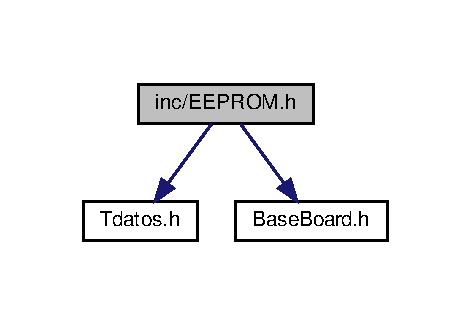
\includegraphics[width=226pt]{d6/d43/EEPROM_8h__incl}
\end{center}
\end{figure}
Gráfico de los archivos que directa o indirectamente incluyen a este archivo\+:\nopagebreak
\begin{figure}[H]
\begin{center}
\leavevmode
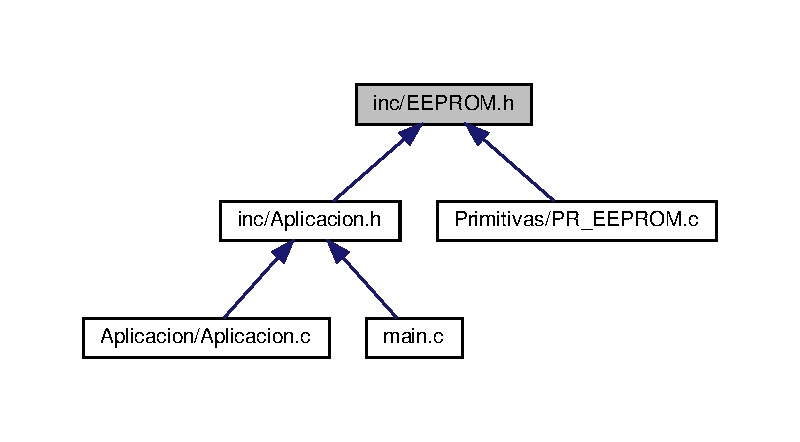
\includegraphics[width=350pt]{d4/d25/EEPROM_8h__dep__incl}
\end{center}
\end{figure}
\subsection*{Funciones}
\begin{DoxyCompactItemize}
\item 
void \hyperlink{EEPROM_8h_ac2f68d23d5b48c9b8bf4f87ccc9ec919}{E\+E\+P\+R\+O\+M\+\_\+\+Write} (\hyperlink{Tdatos_8h_aba7bc1797add20fe3efdf37ced1182c5}{uint8\+\_\+t} addr, \hyperlink{Tdatos_8h_aba7bc1797add20fe3efdf37ced1182c5}{uint8\+\_\+t} n)
\begin{DoxyCompactList}\small\item\em Se encarga de escribir un dato en la memoria E\+E\+P\+R\+OM. \end{DoxyCompactList}\item 
\hyperlink{Tdatos_8h_aba7bc1797add20fe3efdf37ced1182c5}{uint8\+\_\+t} \hyperlink{EEPROM_8h_aefed7e8f08c6375935dec13f4e8d7e6f}{E\+E\+P\+R\+O\+M\+\_\+\+Read} (\hyperlink{Tdatos_8h_aba7bc1797add20fe3efdf37ced1182c5}{uint8\+\_\+t} addr)
\end{DoxyCompactItemize}


\subsection{Documentación de las funciones}
\mbox{\Hypertarget{EEPROM_8h_aefed7e8f08c6375935dec13f4e8d7e6f}\label{EEPROM_8h_aefed7e8f08c6375935dec13f4e8d7e6f}} 
\index{E\+E\+P\+R\+O\+M.\+h@{E\+E\+P\+R\+O\+M.\+h}!E\+E\+P\+R\+O\+M\+\_\+\+Read@{E\+E\+P\+R\+O\+M\+\_\+\+Read}}
\index{E\+E\+P\+R\+O\+M\+\_\+\+Read@{E\+E\+P\+R\+O\+M\+\_\+\+Read}!E\+E\+P\+R\+O\+M.\+h@{E\+E\+P\+R\+O\+M.\+h}}
\subsubsection{\texorpdfstring{E\+E\+P\+R\+O\+M\+\_\+\+Read()}{EEPROM\_Read()}}
{\footnotesize\ttfamily \hyperlink{Tdatos_8h_aba7bc1797add20fe3efdf37ced1182c5}{uint8\+\_\+t} E\+E\+P\+R\+O\+M\+\_\+\+Read (\begin{DoxyParamCaption}\item[{\hyperlink{Tdatos_8h_aba7bc1797add20fe3efdf37ced1182c5}{uint8\+\_\+t}}]{addr }\end{DoxyParamCaption})}



Definición en la línea 117 del archivo P\+R\+\_\+\+E\+E\+P\+R\+O\+M.\+c.

\mbox{\Hypertarget{EEPROM_8h_ac2f68d23d5b48c9b8bf4f87ccc9ec919}\label{EEPROM_8h_ac2f68d23d5b48c9b8bf4f87ccc9ec919}} 
\index{E\+E\+P\+R\+O\+M.\+h@{E\+E\+P\+R\+O\+M.\+h}!E\+E\+P\+R\+O\+M\+\_\+\+Write@{E\+E\+P\+R\+O\+M\+\_\+\+Write}}
\index{E\+E\+P\+R\+O\+M\+\_\+\+Write@{E\+E\+P\+R\+O\+M\+\_\+\+Write}!E\+E\+P\+R\+O\+M.\+h@{E\+E\+P\+R\+O\+M.\+h}}
\subsubsection{\texorpdfstring{E\+E\+P\+R\+O\+M\+\_\+\+Write()}{EEPROM\_Write()}}
{\footnotesize\ttfamily void E\+E\+P\+R\+O\+M\+\_\+\+Write (\begin{DoxyParamCaption}\item[{\hyperlink{Tdatos_8h_aba7bc1797add20fe3efdf37ced1182c5}{uint8\+\_\+t}}]{addr,  }\item[{\hyperlink{Tdatos_8h_aba7bc1797add20fe3efdf37ced1182c5}{uint8\+\_\+t}}]{n }\end{DoxyParamCaption})}



Se encarga de escribir un dato en la memoria E\+E\+P\+R\+OM. 

\begin{DoxyAuthor}{Autor}

\end{DoxyAuthor}
\begin{DoxyDate}{Fecha}

\end{DoxyDate}

\begin{DoxyParams}[1]{Parámetros}
\mbox{\tt in}  & {\em addr} & \\
\hline
\mbox{\tt in}  & {\em n} & \\
\hline
\mbox{\tt out}  & {\em void} & \\
\hline
\end{DoxyParams}


Definición en la línea 85 del archivo P\+R\+\_\+\+E\+E\+P\+R\+O\+M.\+c.


\hypertarget{EncoderIncremental_8h}{}\section{Referencia del Archivo inc/\+Encoder\+Incremental.h}
\label{EncoderIncremental_8h}\index{inc/\+Encoder\+Incremental.\+h@{inc/\+Encoder\+Incremental.\+h}}
{\ttfamily \#include \char`\"{}Tdatos.\+h\char`\"{}}\newline
{\ttfamily \#include \char`\"{}Base\+Board.\+h\char`\"{}}\newline
Dependencia gráfica adjunta para Encoder\+Incremental.\+h\+:\nopagebreak
\begin{figure}[H]
\begin{center}
\leavevmode
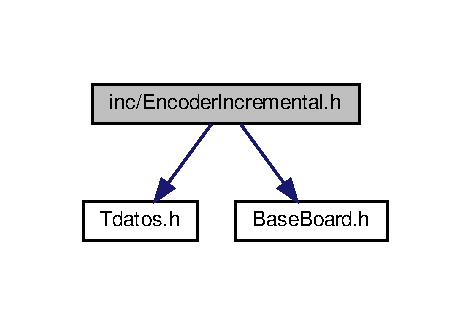
\includegraphics[width=226pt]{dd/d6c/EncoderIncremental_8h__incl}
\end{center}
\end{figure}
Gráfico de los archivos que directa o indirectamente incluyen a este archivo\+:\nopagebreak
\begin{figure}[H]
\begin{center}
\leavevmode
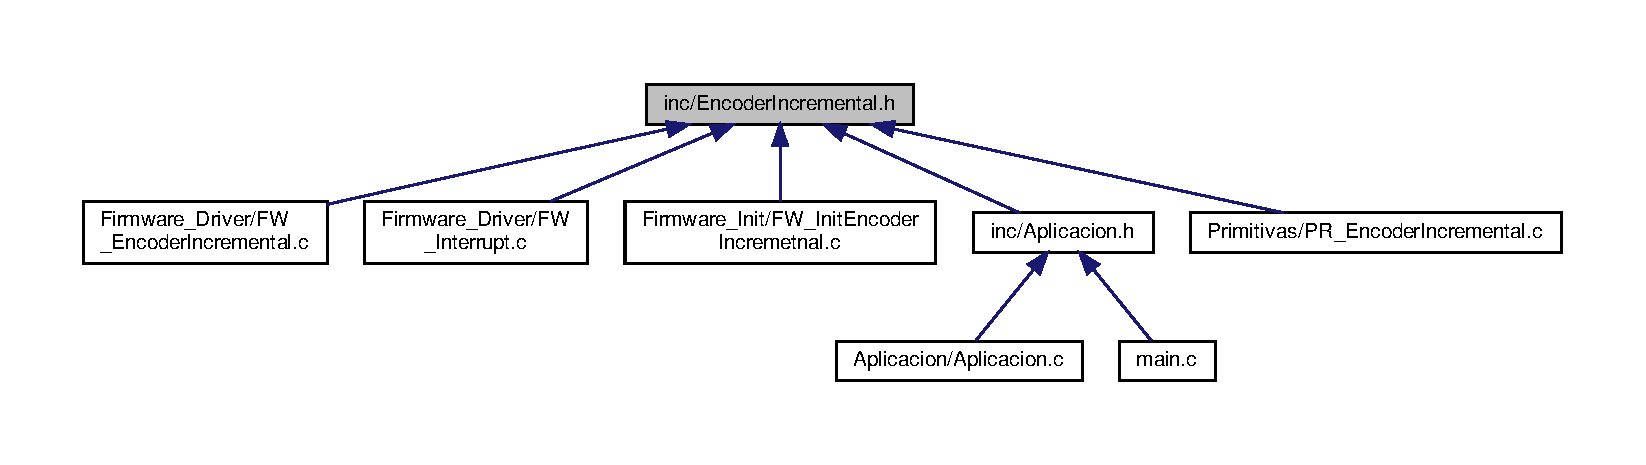
\includegraphics[width=350pt]{d2/da9/EncoderIncremental_8h__dep__incl}
\end{center}
\end{figure}
\subsection*{defines}
\begin{DoxyCompactItemize}
\item 
\#define \hyperlink{EncoderIncremental_8h_ab0986703a2b9b0c1919c4cdcf59148d1}{E\+D\+E\+R\+\_\+\+C\+A\+N\+A\+LA}~P\+O\+R\+T\+Bbits.\+R\+B0
\item 
\#define \hyperlink{EncoderIncremental_8h_a0e0eef9a2c30cd5a7006865dab2d2e79}{E\+D\+E\+R\+\_\+\+C\+A\+N\+A\+LB}~P\+O\+R\+T\+Bbits.\+R\+B1
\item 
\#define \hyperlink{EncoderIncremental_8h_a54aee7bed904715e92c3c6e9f1801f03}{E\+D\+E\+R\+\_\+\+D\+E\+L\+AY}~30
\item 
\#define \hyperlink{EncoderIncremental_8h_a3e68dd4a9bf508ddce011b2113e8ea15}{E\+D\+E\+R\+\_\+\+S\+E\+T\+\_\+\+E\+N\+T\+R\+A\+D\+A\+\_\+A}~T\+R\+I\+S\+Bbits.\+R\+B0 = \hyperlink{BaseBoard_8h_a2267fe6b19995924d44cef4b7d895535}{E\+N\+T\+R\+A\+DA};
\item 
\#define \hyperlink{EncoderIncremental_8h_af92c80b05580f3d5515455f8623ad33f}{E\+D\+E\+R\+\_\+\+S\+E\+T\+\_\+\+E\+N\+T\+R\+A\+D\+A\+\_\+B}~T\+R\+I\+S\+Bbits.\+R\+B1 = \hyperlink{BaseBoard_8h_a2267fe6b19995924d44cef4b7d895535}{E\+N\+T\+R\+A\+DA};
\end{DoxyCompactItemize}
\subsection*{Funciones}
\begin{DoxyCompactItemize}
\item 
void \hyperlink{EncoderIncremental_8h_a1f92e3491d1d96007589f41b5eb03fe7}{E\+D\+E\+R\+\_\+\+Init} (\hyperlink{Tdatos_8h_aba7bc1797add20fe3efdf37ced1182c5}{uint8\+\_\+t} set\+M\+AX, \hyperlink{Tdatos_8h_aba7bc1797add20fe3efdf37ced1182c5}{uint8\+\_\+t} set\+Min)
\begin{DoxyCompactList}\small\item\em Funcion necesaria para inicializar el encoder, en la misma se define el rango del encoder. \end{DoxyCompactList}\item 
\hyperlink{Tdatos_8h_aba7bc1797add20fe3efdf37ced1182c5}{uint8\+\_\+t} \hyperlink{EncoderIncremental_8h_a1180a1403bc1363e30af38b9c276a9ea}{E\+D\+E\+R\+\_\+\+Get\+Pos} (void)
\begin{DoxyCompactList}\small\item\em Llamando a esta funcion se obtiene un numero entre el valor M\+AX y el min. \end{DoxyCompactList}\item 
void \hyperlink{EncoderIncremental_8h_a84d2929e16ed8c23f50ad0148163267f}{E\+D\+E\+R\+\_\+\+Put\+Pos} (unsigned char posicion)
\begin{DoxyCompactList}\small\item\em Llamando a esta funcion se inicializa la posicion del encoder. \end{DoxyCompactList}\item 
void \hyperlink{EncoderIncremental_8h_a90a4d0e96e4a9aac93bb2b59e2f1b624}{E\+D\+E\+R\+\_\+\+Interrupt} (void)
\item 
void \hyperlink{EncoderIncremental_8h_a11701efeb48e9b7b95efe7a958a91401}{E\+D\+E\+R\+\_\+\+Tic} (void)
\begin{DoxyCompactList}\small\item\em Se encarga de la demora. \end{DoxyCompactList}\end{DoxyCompactItemize}
\subsection*{Variables}
\begin{DoxyCompactItemize}
\item 
volatile \hyperlink{Tdatos_8h_aba7bc1797add20fe3efdf37ced1182c5}{uint8\+\_\+t} \hyperlink{EncoderIncremental_8h_acba4a26c0330eb8f52158e306351fd67}{E\+D\+E\+R\+\_\+\+Maximo}
\item 
volatile \hyperlink{Tdatos_8h_aba7bc1797add20fe3efdf37ced1182c5}{uint8\+\_\+t} \hyperlink{EncoderIncremental_8h_a60645d94d942d68dd1c4a5d039df5860}{E\+D\+E\+R\+\_\+\+Minimo}
\item 
volatile \hyperlink{Tdatos_8h_aba7bc1797add20fe3efdf37ced1182c5}{uint8\+\_\+t} \hyperlink{EncoderIncremental_8h_a7a16d365adb64dd67685e78369350faf}{E\+D\+E\+R\+\_\+\+Delay}
\item 
volatile \hyperlink{Tdatos_8h_aba7bc1797add20fe3efdf37ced1182c5}{uint8\+\_\+t} \hyperlink{EncoderIncremental_8h_a677c386c12bb126117ae9bde73d296e2}{E\+D\+E\+R\+\_\+\+Posicion}
\item 
volatile \hyperlink{Tdatos_8h_aba7bc1797add20fe3efdf37ced1182c5}{uint8\+\_\+t} \hyperlink{EncoderIncremental_8h_acec90ea3b9fe87fc336faf998a18f74a}{E\+D\+E\+R\+\_\+\+Flag\+Canal}
\end{DoxyCompactItemize}


\subsection{Documentación de los \textquotesingle{}defines\textquotesingle{}}
\mbox{\Hypertarget{EncoderIncremental_8h_ab0986703a2b9b0c1919c4cdcf59148d1}\label{EncoderIncremental_8h_ab0986703a2b9b0c1919c4cdcf59148d1}} 
\index{Encoder\+Incremental.\+h@{Encoder\+Incremental.\+h}!E\+D\+E\+R\+\_\+\+C\+A\+N\+A\+LA@{E\+D\+E\+R\+\_\+\+C\+A\+N\+A\+LA}}
\index{E\+D\+E\+R\+\_\+\+C\+A\+N\+A\+LA@{E\+D\+E\+R\+\_\+\+C\+A\+N\+A\+LA}!Encoder\+Incremental.\+h@{Encoder\+Incremental.\+h}}
\subsubsection{\texorpdfstring{E\+D\+E\+R\+\_\+\+C\+A\+N\+A\+LA}{EDER\_CANALA}}
{\footnotesize\ttfamily \#define E\+D\+E\+R\+\_\+\+C\+A\+N\+A\+LA~P\+O\+R\+T\+Bbits.\+R\+B0}



Definición en la línea 51 del archivo Encoder\+Incremental.\+h.

\mbox{\Hypertarget{EncoderIncremental_8h_a0e0eef9a2c30cd5a7006865dab2d2e79}\label{EncoderIncremental_8h_a0e0eef9a2c30cd5a7006865dab2d2e79}} 
\index{Encoder\+Incremental.\+h@{Encoder\+Incremental.\+h}!E\+D\+E\+R\+\_\+\+C\+A\+N\+A\+LB@{E\+D\+E\+R\+\_\+\+C\+A\+N\+A\+LB}}
\index{E\+D\+E\+R\+\_\+\+C\+A\+N\+A\+LB@{E\+D\+E\+R\+\_\+\+C\+A\+N\+A\+LB}!Encoder\+Incremental.\+h@{Encoder\+Incremental.\+h}}
\subsubsection{\texorpdfstring{E\+D\+E\+R\+\_\+\+C\+A\+N\+A\+LB}{EDER\_CANALB}}
{\footnotesize\ttfamily \#define E\+D\+E\+R\+\_\+\+C\+A\+N\+A\+LB~P\+O\+R\+T\+Bbits.\+R\+B1}



Definición en la línea 52 del archivo Encoder\+Incremental.\+h.

\mbox{\Hypertarget{EncoderIncremental_8h_a54aee7bed904715e92c3c6e9f1801f03}\label{EncoderIncremental_8h_a54aee7bed904715e92c3c6e9f1801f03}} 
\index{Encoder\+Incremental.\+h@{Encoder\+Incremental.\+h}!E\+D\+E\+R\+\_\+\+D\+E\+L\+AY@{E\+D\+E\+R\+\_\+\+D\+E\+L\+AY}}
\index{E\+D\+E\+R\+\_\+\+D\+E\+L\+AY@{E\+D\+E\+R\+\_\+\+D\+E\+L\+AY}!Encoder\+Incremental.\+h@{Encoder\+Incremental.\+h}}
\subsubsection{\texorpdfstring{E\+D\+E\+R\+\_\+\+D\+E\+L\+AY}{EDER\_DELAY}}
{\footnotesize\ttfamily \#define E\+D\+E\+R\+\_\+\+D\+E\+L\+AY~30}



Definición en la línea 53 del archivo Encoder\+Incremental.\+h.

\mbox{\Hypertarget{EncoderIncremental_8h_a3e68dd4a9bf508ddce011b2113e8ea15}\label{EncoderIncremental_8h_a3e68dd4a9bf508ddce011b2113e8ea15}} 
\index{Encoder\+Incremental.\+h@{Encoder\+Incremental.\+h}!E\+D\+E\+R\+\_\+\+S\+E\+T\+\_\+\+E\+N\+T\+R\+A\+D\+A\+\_\+A@{E\+D\+E\+R\+\_\+\+S\+E\+T\+\_\+\+E\+N\+T\+R\+A\+D\+A\+\_\+A}}
\index{E\+D\+E\+R\+\_\+\+S\+E\+T\+\_\+\+E\+N\+T\+R\+A\+D\+A\+\_\+A@{E\+D\+E\+R\+\_\+\+S\+E\+T\+\_\+\+E\+N\+T\+R\+A\+D\+A\+\_\+A}!Encoder\+Incremental.\+h@{Encoder\+Incremental.\+h}}
\subsubsection{\texorpdfstring{E\+D\+E\+R\+\_\+\+S\+E\+T\+\_\+\+E\+N\+T\+R\+A\+D\+A\+\_\+A}{EDER\_SET\_ENTRADA\_A}}
{\footnotesize\ttfamily \#define E\+D\+E\+R\+\_\+\+S\+E\+T\+\_\+\+E\+N\+T\+R\+A\+D\+A\+\_\+A~T\+R\+I\+S\+Bbits.\+R\+B0 = \hyperlink{BaseBoard_8h_a2267fe6b19995924d44cef4b7d895535}{E\+N\+T\+R\+A\+DA};}



Definición en la línea 59 del archivo Encoder\+Incremental.\+h.

\mbox{\Hypertarget{EncoderIncremental_8h_af92c80b05580f3d5515455f8623ad33f}\label{EncoderIncremental_8h_af92c80b05580f3d5515455f8623ad33f}} 
\index{Encoder\+Incremental.\+h@{Encoder\+Incremental.\+h}!E\+D\+E\+R\+\_\+\+S\+E\+T\+\_\+\+E\+N\+T\+R\+A\+D\+A\+\_\+B@{E\+D\+E\+R\+\_\+\+S\+E\+T\+\_\+\+E\+N\+T\+R\+A\+D\+A\+\_\+B}}
\index{E\+D\+E\+R\+\_\+\+S\+E\+T\+\_\+\+E\+N\+T\+R\+A\+D\+A\+\_\+B@{E\+D\+E\+R\+\_\+\+S\+E\+T\+\_\+\+E\+N\+T\+R\+A\+D\+A\+\_\+B}!Encoder\+Incremental.\+h@{Encoder\+Incremental.\+h}}
\subsubsection{\texorpdfstring{E\+D\+E\+R\+\_\+\+S\+E\+T\+\_\+\+E\+N\+T\+R\+A\+D\+A\+\_\+B}{EDER\_SET\_ENTRADA\_B}}
{\footnotesize\ttfamily \#define E\+D\+E\+R\+\_\+\+S\+E\+T\+\_\+\+E\+N\+T\+R\+A\+D\+A\+\_\+B~T\+R\+I\+S\+Bbits.\+R\+B1 = \hyperlink{BaseBoard_8h_a2267fe6b19995924d44cef4b7d895535}{E\+N\+T\+R\+A\+DA};}



Definición en la línea 60 del archivo Encoder\+Incremental.\+h.



\subsection{Documentación de las funciones}
\mbox{\Hypertarget{EncoderIncremental_8h_a1180a1403bc1363e30af38b9c276a9ea}\label{EncoderIncremental_8h_a1180a1403bc1363e30af38b9c276a9ea}} 
\index{Encoder\+Incremental.\+h@{Encoder\+Incremental.\+h}!E\+D\+E\+R\+\_\+\+Get\+Pos@{E\+D\+E\+R\+\_\+\+Get\+Pos}}
\index{E\+D\+E\+R\+\_\+\+Get\+Pos@{E\+D\+E\+R\+\_\+\+Get\+Pos}!Encoder\+Incremental.\+h@{Encoder\+Incremental.\+h}}
\subsubsection{\texorpdfstring{E\+D\+E\+R\+\_\+\+Get\+Pos()}{EDER\_GetPos()}}
{\footnotesize\ttfamily \hyperlink{Tdatos_8h_aba7bc1797add20fe3efdf37ced1182c5}{uint8\+\_\+t} E\+D\+E\+R\+\_\+\+Get\+Pos (\begin{DoxyParamCaption}\item[{void}]{ }\end{DoxyParamCaption})}



Llamando a esta funcion se obtiene un numero entre el valor M\+AX y el min. 

\begin{DoxyAuthor}{Autor}

\end{DoxyAuthor}
\begin{DoxyDate}{Fecha}

\end{DoxyDate}

\begin{DoxyParams}[1]{Parámetros}
\mbox{\tt in}  & {\em void} & \\
\hline
\mbox{\tt out}  & {\em posicion\+\_\+encoder} & uint8\+\_\+t \\
\hline
\end{DoxyParams}


Definición en la línea 90 del archivo P\+R\+\_\+\+Encoder\+Incremental.\+c.

\mbox{\Hypertarget{EncoderIncremental_8h_a1f92e3491d1d96007589f41b5eb03fe7}\label{EncoderIncremental_8h_a1f92e3491d1d96007589f41b5eb03fe7}} 
\index{Encoder\+Incremental.\+h@{Encoder\+Incremental.\+h}!E\+D\+E\+R\+\_\+\+Init@{E\+D\+E\+R\+\_\+\+Init}}
\index{E\+D\+E\+R\+\_\+\+Init@{E\+D\+E\+R\+\_\+\+Init}!Encoder\+Incremental.\+h@{Encoder\+Incremental.\+h}}
\subsubsection{\texorpdfstring{E\+D\+E\+R\+\_\+\+Init()}{EDER\_Init()}}
{\footnotesize\ttfamily void E\+D\+E\+R\+\_\+\+Init (\begin{DoxyParamCaption}\item[{\hyperlink{Tdatos_8h_aba7bc1797add20fe3efdf37ced1182c5}{uint8\+\_\+t}}]{set\+M\+AX,  }\item[{\hyperlink{Tdatos_8h_aba7bc1797add20fe3efdf37ced1182c5}{uint8\+\_\+t}}]{set\+Min }\end{DoxyParamCaption})}



Funcion necesaria para inicializar el encoder, en la misma se define el rango del encoder. 

\begin{DoxyAuthor}{Autor}

\end{DoxyAuthor}
\begin{DoxyDate}{Fecha}

\end{DoxyDate}

\begin{DoxyParams}[1]{Parámetros}
\mbox{\tt in}  & {\em set\+M\+AX} & necesario para definir la posicion maxima \\
\hline
\mbox{\tt in}  & {\em set\+Min} & necesario para definir la posicion minima \\
\hline
\mbox{\tt out}  & {\em void} & \\
\hline
\end{DoxyParams}


Definición en la línea 93 del archivo F\+W\+\_\+\+Init\+Encoder\+Incremetnal.\+c.

\mbox{\Hypertarget{EncoderIncremental_8h_a90a4d0e96e4a9aac93bb2b59e2f1b624}\label{EncoderIncremental_8h_a90a4d0e96e4a9aac93bb2b59e2f1b624}} 
\index{Encoder\+Incremental.\+h@{Encoder\+Incremental.\+h}!E\+D\+E\+R\+\_\+\+Interrupt@{E\+D\+E\+R\+\_\+\+Interrupt}}
\index{E\+D\+E\+R\+\_\+\+Interrupt@{E\+D\+E\+R\+\_\+\+Interrupt}!Encoder\+Incremental.\+h@{Encoder\+Incremental.\+h}}
\subsubsection{\texorpdfstring{E\+D\+E\+R\+\_\+\+Interrupt()}{EDER\_Interrupt()}}
{\footnotesize\ttfamily void E\+D\+E\+R\+\_\+\+Interrupt (\begin{DoxyParamCaption}\item[{void}]{ }\end{DoxyParamCaption})}



Definición en la línea 113 del archivo F\+W\+\_\+\+Encoder\+Incremental.\+c.

\mbox{\Hypertarget{EncoderIncremental_8h_a84d2929e16ed8c23f50ad0148163267f}\label{EncoderIncremental_8h_a84d2929e16ed8c23f50ad0148163267f}} 
\index{Encoder\+Incremental.\+h@{Encoder\+Incremental.\+h}!E\+D\+E\+R\+\_\+\+Put\+Pos@{E\+D\+E\+R\+\_\+\+Put\+Pos}}
\index{E\+D\+E\+R\+\_\+\+Put\+Pos@{E\+D\+E\+R\+\_\+\+Put\+Pos}!Encoder\+Incremental.\+h@{Encoder\+Incremental.\+h}}
\subsubsection{\texorpdfstring{E\+D\+E\+R\+\_\+\+Put\+Pos()}{EDER\_PutPos()}}
{\footnotesize\ttfamily void E\+D\+E\+R\+\_\+\+Put\+Pos (\begin{DoxyParamCaption}\item[{unsigned char}]{posicion }\end{DoxyParamCaption})}



Llamando a esta funcion se inicializa la posicion del encoder. 

\begin{DoxyAuthor}{Autor}

\end{DoxyAuthor}
\begin{DoxyDate}{Fecha}

\end{DoxyDate}

\begin{DoxyParams}[1]{Parámetros}
\mbox{\tt in}  & {\em posicion} & indica que posicion tiene el encoder fisicamente \\
\hline
\mbox{\tt out}  & {\em void} & \\
\hline
\end{DoxyParams}


Definición en la línea 104 del archivo P\+R\+\_\+\+Encoder\+Incremental.\+c.

\mbox{\Hypertarget{EncoderIncremental_8h_a11701efeb48e9b7b95efe7a958a91401}\label{EncoderIncremental_8h_a11701efeb48e9b7b95efe7a958a91401}} 
\index{Encoder\+Incremental.\+h@{Encoder\+Incremental.\+h}!E\+D\+E\+R\+\_\+\+Tic@{E\+D\+E\+R\+\_\+\+Tic}}
\index{E\+D\+E\+R\+\_\+\+Tic@{E\+D\+E\+R\+\_\+\+Tic}!Encoder\+Incremental.\+h@{Encoder\+Incremental.\+h}}
\subsubsection{\texorpdfstring{E\+D\+E\+R\+\_\+\+Tic()}{EDER\_Tic()}}
{\footnotesize\ttfamily void E\+D\+E\+R\+\_\+\+Tic (\begin{DoxyParamCaption}\item[{void}]{ }\end{DoxyParamCaption})}



Se encarga de la demora. 

\begin{DoxyAuthor}{Autor}

\end{DoxyAuthor}
\begin{DoxyDate}{Fecha}

\end{DoxyDate}

\begin{DoxyParams}[1]{Parámetros}
\mbox{\tt in}  & {\em void} & \\
\hline
\mbox{\tt out}  & {\em void} & \\
\hline
\end{DoxyParams}


Definición en la línea 145 del archivo F\+W\+\_\+\+Encoder\+Incremental.\+c.



\subsection{Documentación de las variables}
\mbox{\Hypertarget{EncoderIncremental_8h_a7a16d365adb64dd67685e78369350faf}\label{EncoderIncremental_8h_a7a16d365adb64dd67685e78369350faf}} 
\index{Encoder\+Incremental.\+h@{Encoder\+Incremental.\+h}!E\+D\+E\+R\+\_\+\+Delay@{E\+D\+E\+R\+\_\+\+Delay}}
\index{E\+D\+E\+R\+\_\+\+Delay@{E\+D\+E\+R\+\_\+\+Delay}!Encoder\+Incremental.\+h@{Encoder\+Incremental.\+h}}
\subsubsection{\texorpdfstring{E\+D\+E\+R\+\_\+\+Delay}{EDER\_Delay}}
{\footnotesize\ttfamily volatile \hyperlink{Tdatos_8h_aba7bc1797add20fe3efdf37ced1182c5}{uint8\+\_\+t} E\+D\+E\+R\+\_\+\+Delay}



Definición en la línea 67 del archivo F\+W\+\_\+\+Encoder\+Incremental.\+c.

\mbox{\Hypertarget{EncoderIncremental_8h_acec90ea3b9fe87fc336faf998a18f74a}\label{EncoderIncremental_8h_acec90ea3b9fe87fc336faf998a18f74a}} 
\index{Encoder\+Incremental.\+h@{Encoder\+Incremental.\+h}!E\+D\+E\+R\+\_\+\+Flag\+Canal@{E\+D\+E\+R\+\_\+\+Flag\+Canal}}
\index{E\+D\+E\+R\+\_\+\+Flag\+Canal@{E\+D\+E\+R\+\_\+\+Flag\+Canal}!Encoder\+Incremental.\+h@{Encoder\+Incremental.\+h}}
\subsubsection{\texorpdfstring{E\+D\+E\+R\+\_\+\+Flag\+Canal}{EDER\_FlagCanal}}
{\footnotesize\ttfamily volatile \hyperlink{Tdatos_8h_aba7bc1797add20fe3efdf37ced1182c5}{uint8\+\_\+t} E\+D\+E\+R\+\_\+\+Flag\+Canal}



Definición en la línea 68 del archivo F\+W\+\_\+\+Encoder\+Incremental.\+c.

\mbox{\Hypertarget{EncoderIncremental_8h_acba4a26c0330eb8f52158e306351fd67}\label{EncoderIncremental_8h_acba4a26c0330eb8f52158e306351fd67}} 
\index{Encoder\+Incremental.\+h@{Encoder\+Incremental.\+h}!E\+D\+E\+R\+\_\+\+Maximo@{E\+D\+E\+R\+\_\+\+Maximo}}
\index{E\+D\+E\+R\+\_\+\+Maximo@{E\+D\+E\+R\+\_\+\+Maximo}!Encoder\+Incremental.\+h@{Encoder\+Incremental.\+h}}
\subsubsection{\texorpdfstring{E\+D\+E\+R\+\_\+\+Maximo}{EDER\_Maximo}}
{\footnotesize\ttfamily volatile \hyperlink{Tdatos_8h_aba7bc1797add20fe3efdf37ced1182c5}{uint8\+\_\+t} E\+D\+E\+R\+\_\+\+Maximo}



Definición en la línea 68 del archivo F\+W\+\_\+\+Init\+Encoder\+Incremetnal.\+c.

\mbox{\Hypertarget{EncoderIncremental_8h_a60645d94d942d68dd1c4a5d039df5860}\label{EncoderIncremental_8h_a60645d94d942d68dd1c4a5d039df5860}} 
\index{Encoder\+Incremental.\+h@{Encoder\+Incremental.\+h}!E\+D\+E\+R\+\_\+\+Minimo@{E\+D\+E\+R\+\_\+\+Minimo}}
\index{E\+D\+E\+R\+\_\+\+Minimo@{E\+D\+E\+R\+\_\+\+Minimo}!Encoder\+Incremental.\+h@{Encoder\+Incremental.\+h}}
\subsubsection{\texorpdfstring{E\+D\+E\+R\+\_\+\+Minimo}{EDER\_Minimo}}
{\footnotesize\ttfamily volatile \hyperlink{Tdatos_8h_aba7bc1797add20fe3efdf37ced1182c5}{uint8\+\_\+t} E\+D\+E\+R\+\_\+\+Minimo}



Definición en la línea 69 del archivo F\+W\+\_\+\+Init\+Encoder\+Incremetnal.\+c.

\mbox{\Hypertarget{EncoderIncremental_8h_a677c386c12bb126117ae9bde73d296e2}\label{EncoderIncremental_8h_a677c386c12bb126117ae9bde73d296e2}} 
\index{Encoder\+Incremental.\+h@{Encoder\+Incremental.\+h}!E\+D\+E\+R\+\_\+\+Posicion@{E\+D\+E\+R\+\_\+\+Posicion}}
\index{E\+D\+E\+R\+\_\+\+Posicion@{E\+D\+E\+R\+\_\+\+Posicion}!Encoder\+Incremental.\+h@{Encoder\+Incremental.\+h}}
\subsubsection{\texorpdfstring{E\+D\+E\+R\+\_\+\+Posicion}{EDER\_Posicion}}
{\footnotesize\ttfamily volatile \hyperlink{Tdatos_8h_aba7bc1797add20fe3efdf37ced1182c5}{uint8\+\_\+t} E\+D\+E\+R\+\_\+\+Posicion}



Definición en la línea 67 del archivo P\+R\+\_\+\+Encoder\+Incremental.\+c.


\hypertarget{EntradasDigitales_8h}{}\section{Referencia del Archivo inc/\+Entradas\+Digitales.h}
\label{EntradasDigitales_8h}\index{inc/\+Entradas\+Digitales.\+h@{inc/\+Entradas\+Digitales.\+h}}
{\ttfamily \#include \char`\"{}Tdatos.\+h\char`\"{}}\newline
{\ttfamily \#include \char`\"{}Base\+Board.\+h\char`\"{}}\newline
Dependencia gráfica adjunta para Entradas\+Digitales.\+h\+:\nopagebreak
\begin{figure}[H]
\begin{center}
\leavevmode
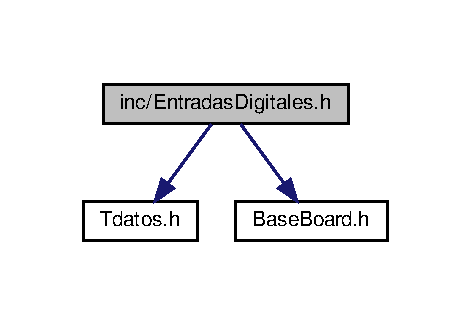
\includegraphics[width=226pt]{df/df5/EntradasDigitales_8h__incl}
\end{center}
\end{figure}
Gráfico de los archivos que directa o indirectamente incluyen a este archivo\+:\nopagebreak
\begin{figure}[H]
\begin{center}
\leavevmode
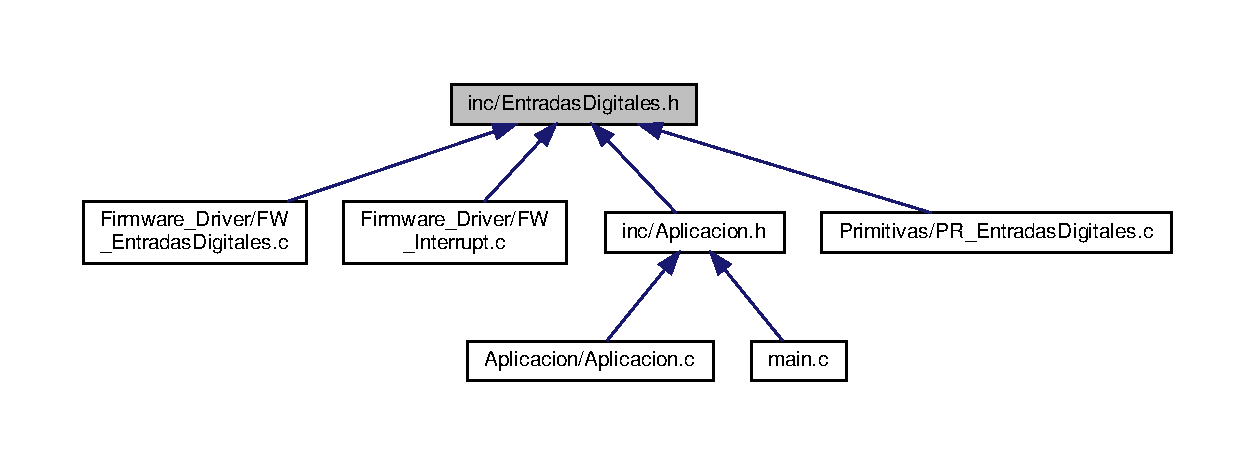
\includegraphics[width=350pt]{dc/d56/EntradasDigitales_8h__dep__incl}
\end{center}
\end{figure}
\subsection*{defines}
\begin{DoxyCompactItemize}
\item 
\#define \hyperlink{EntradasDigitales_8h_ae25ec654c4dabac685454a7263985649}{E\+D\+\_\+\+A\+C\+E\+P\+T\+A\+R\+\_\+\+E\+S\+T\+A\+DO}~10
\begin{DoxyCompactList}\small\item\em cantidad de veces que deve contar para validar el estado \end{DoxyCompactList}\item 
\#define \hyperlink{EntradasDigitales_8h_a31160dcd18f4f23a10b24c17fd7d0081}{E\+D\+\_\+\+E\+N\+T\+R\+A\+D\+AS}~4
\begin{DoxyCompactList}\small\item\em cantidad de entradas \end{DoxyCompactList}\item 
\#define \hyperlink{EntradasDigitales_8h_a63fb786778d627ac652386fea3980b26}{E\+D\+\_\+\+T\+IC}~1
\item 
\#define \hyperlink{EntradasDigitales_8h_a4dfc73e8376485479b6d2250a0446da2}{E\+D\+\_\+\+T\+E\+C\+L\+A0}~(\hyperlink{Tdatos_8h_aba7bc1797add20fe3efdf37ced1182c5}{uint8\+\_\+t})((\hyperlink{PR__EntradasDigitales_8c_a563d13d1151e7bc19b8c505ac9d4a33e}{E\+D\+\_\+\+Buffer\+Entradas}) \& 0x01)
\begin{DoxyCompactList}\small\item\em macros para las teclas de entrada \end{DoxyCompactList}\item 
\#define \hyperlink{EntradasDigitales_8h_accbf3ae157416e23f1142534ee302b93}{E\+D\+\_\+\+T\+E\+C\+L\+A1}~(\hyperlink{Tdatos_8h_aba7bc1797add20fe3efdf37ced1182c5}{uint8\+\_\+t})((\hyperlink{PR__EntradasDigitales_8c_a563d13d1151e7bc19b8c505ac9d4a33e}{E\+D\+\_\+\+Buffer\+Entradas} $>$$>$ 1) \& 0x01)
\begin{DoxyCompactList}\small\item\em macros para las teclas de entrada \end{DoxyCompactList}\item 
\#define \hyperlink{EntradasDigitales_8h_acf90b94c3ed6506779f0870b596196be}{E\+D\+\_\+\+T\+E\+C\+L\+A2}~(\hyperlink{Tdatos_8h_aba7bc1797add20fe3efdf37ced1182c5}{uint8\+\_\+t})((\hyperlink{PR__EntradasDigitales_8c_a563d13d1151e7bc19b8c505ac9d4a33e}{E\+D\+\_\+\+Buffer\+Entradas} $>$$>$ 2) \& 0x01)
\begin{DoxyCompactList}\small\item\em macros para las teclas de entrada \end{DoxyCompactList}\item 
\#define \hyperlink{EntradasDigitales_8h_ad0a2f09b98b2d52f04e698c4ec7252b6}{E\+D\+\_\+\+T\+E\+C\+L\+A3}~(\hyperlink{Tdatos_8h_aba7bc1797add20fe3efdf37ced1182c5}{uint8\+\_\+t})((\hyperlink{PR__EntradasDigitales_8c_a563d13d1151e7bc19b8c505ac9d4a33e}{E\+D\+\_\+\+Buffer\+Entradas} $>$$>$ 3) \& 0x01)
\begin{DoxyCompactList}\small\item\em macros para las teclas de entrada \end{DoxyCompactList}\end{DoxyCompactItemize}
\subsection*{Funciones}
\begin{DoxyCompactItemize}
\item 
void \hyperlink{EntradasDigitales_8h_a4a160ca6fd77d23f27dd9b6af1b3a35e}{E\+D\+\_\+\+Cuenta\+Pulsos} (void)
\begin{DoxyCompactList}\small\item\em Funcion primitiva de entradas digitales. \end{DoxyCompactList}\item 
void \hyperlink{EntradasDigitales_8h_aae3299a4d1a16965cb68fdb0dfe20a2a}{E\+D\+\_\+\+Debounce} (void)
\begin{DoxyCompactList}\small\item\em Funcion para el debounce de las entradas digitales. \end{DoxyCompactList}\item 
void \hyperlink{EntradasDigitales_8h_a37cb4f85d5ecd1e06ebee2aff2cea677}{E\+D\+\_\+\+Tic} (void)
\begin{DoxyCompactList}\small\item\em Funcion para el debounce de las entradas digitales. \end{DoxyCompactList}\end{DoxyCompactItemize}
\subsection*{Variables}
\begin{DoxyCompactItemize}
\item 
volatile \hyperlink{Tdatos_8h_aba7bc1797add20fe3efdf37ced1182c5}{uint8\+\_\+t} \hyperlink{EntradasDigitales_8h_a563d13d1151e7bc19b8c505ac9d4a33e}{E\+D\+\_\+\+Buffer\+Entradas}
\begin{DoxyCompactList}\small\item\em aca por cada bit me indica el estado de una tecla \end{DoxyCompactList}\item 
volatile \hyperlink{Tdatos_8h_aba7bc1797add20fe3efdf37ced1182c5}{uint8\+\_\+t} \hyperlink{EntradasDigitales_8h_a85bf28760a0b8f0d354faa8e0560a4f8}{E\+D\+\_\+\+Delay}
\end{DoxyCompactItemize}


\subsection{Documentación de los \textquotesingle{}defines\textquotesingle{}}
\mbox{\Hypertarget{EntradasDigitales_8h_ae25ec654c4dabac685454a7263985649}\label{EntradasDigitales_8h_ae25ec654c4dabac685454a7263985649}} 
\index{Entradas\+Digitales.\+h@{Entradas\+Digitales.\+h}!E\+D\+\_\+\+A\+C\+E\+P\+T\+A\+R\+\_\+\+E\+S\+T\+A\+DO@{E\+D\+\_\+\+A\+C\+E\+P\+T\+A\+R\+\_\+\+E\+S\+T\+A\+DO}}
\index{E\+D\+\_\+\+A\+C\+E\+P\+T\+A\+R\+\_\+\+E\+S\+T\+A\+DO@{E\+D\+\_\+\+A\+C\+E\+P\+T\+A\+R\+\_\+\+E\+S\+T\+A\+DO}!Entradas\+Digitales.\+h@{Entradas\+Digitales.\+h}}
\subsubsection{\texorpdfstring{E\+D\+\_\+\+A\+C\+E\+P\+T\+A\+R\+\_\+\+E\+S\+T\+A\+DO}{ED\_ACEPTAR\_ESTADO}}
{\footnotesize\ttfamily \#define E\+D\+\_\+\+A\+C\+E\+P\+T\+A\+R\+\_\+\+E\+S\+T\+A\+DO~10}



cantidad de veces que deve contar para validar el estado 



Definición en la línea 54 del archivo Entradas\+Digitales.\+h.

\mbox{\Hypertarget{EntradasDigitales_8h_a31160dcd18f4f23a10b24c17fd7d0081}\label{EntradasDigitales_8h_a31160dcd18f4f23a10b24c17fd7d0081}} 
\index{Entradas\+Digitales.\+h@{Entradas\+Digitales.\+h}!E\+D\+\_\+\+E\+N\+T\+R\+A\+D\+AS@{E\+D\+\_\+\+E\+N\+T\+R\+A\+D\+AS}}
\index{E\+D\+\_\+\+E\+N\+T\+R\+A\+D\+AS@{E\+D\+\_\+\+E\+N\+T\+R\+A\+D\+AS}!Entradas\+Digitales.\+h@{Entradas\+Digitales.\+h}}
\subsubsection{\texorpdfstring{E\+D\+\_\+\+E\+N\+T\+R\+A\+D\+AS}{ED\_ENTRADAS}}
{\footnotesize\ttfamily \#define E\+D\+\_\+\+E\+N\+T\+R\+A\+D\+AS~4}



cantidad de entradas 



Definición en la línea 55 del archivo Entradas\+Digitales.\+h.

\mbox{\Hypertarget{EntradasDigitales_8h_a4dfc73e8376485479b6d2250a0446da2}\label{EntradasDigitales_8h_a4dfc73e8376485479b6d2250a0446da2}} 
\index{Entradas\+Digitales.\+h@{Entradas\+Digitales.\+h}!E\+D\+\_\+\+T\+E\+C\+L\+A0@{E\+D\+\_\+\+T\+E\+C\+L\+A0}}
\index{E\+D\+\_\+\+T\+E\+C\+L\+A0@{E\+D\+\_\+\+T\+E\+C\+L\+A0}!Entradas\+Digitales.\+h@{Entradas\+Digitales.\+h}}
\subsubsection{\texorpdfstring{E\+D\+\_\+\+T\+E\+C\+L\+A0}{ED\_TECLA0}}
{\footnotesize\ttfamily \#define E\+D\+\_\+\+T\+E\+C\+L\+A0~(\hyperlink{Tdatos_8h_aba7bc1797add20fe3efdf37ced1182c5}{uint8\+\_\+t})((\hyperlink{PR__EntradasDigitales_8c_a563d13d1151e7bc19b8c505ac9d4a33e}{E\+D\+\_\+\+Buffer\+Entradas}) \& 0x01)}



macros para las teclas de entrada 



Definición en la línea 58 del archivo Entradas\+Digitales.\+h.

\mbox{\Hypertarget{EntradasDigitales_8h_accbf3ae157416e23f1142534ee302b93}\label{EntradasDigitales_8h_accbf3ae157416e23f1142534ee302b93}} 
\index{Entradas\+Digitales.\+h@{Entradas\+Digitales.\+h}!E\+D\+\_\+\+T\+E\+C\+L\+A1@{E\+D\+\_\+\+T\+E\+C\+L\+A1}}
\index{E\+D\+\_\+\+T\+E\+C\+L\+A1@{E\+D\+\_\+\+T\+E\+C\+L\+A1}!Entradas\+Digitales.\+h@{Entradas\+Digitales.\+h}}
\subsubsection{\texorpdfstring{E\+D\+\_\+\+T\+E\+C\+L\+A1}{ED\_TECLA1}}
{\footnotesize\ttfamily \#define E\+D\+\_\+\+T\+E\+C\+L\+A1~(\hyperlink{Tdatos_8h_aba7bc1797add20fe3efdf37ced1182c5}{uint8\+\_\+t})((\hyperlink{PR__EntradasDigitales_8c_a563d13d1151e7bc19b8c505ac9d4a33e}{E\+D\+\_\+\+Buffer\+Entradas} $>$$>$ 1) \& 0x01)}



macros para las teclas de entrada 



Definición en la línea 59 del archivo Entradas\+Digitales.\+h.

\mbox{\Hypertarget{EntradasDigitales_8h_acf90b94c3ed6506779f0870b596196be}\label{EntradasDigitales_8h_acf90b94c3ed6506779f0870b596196be}} 
\index{Entradas\+Digitales.\+h@{Entradas\+Digitales.\+h}!E\+D\+\_\+\+T\+E\+C\+L\+A2@{E\+D\+\_\+\+T\+E\+C\+L\+A2}}
\index{E\+D\+\_\+\+T\+E\+C\+L\+A2@{E\+D\+\_\+\+T\+E\+C\+L\+A2}!Entradas\+Digitales.\+h@{Entradas\+Digitales.\+h}}
\subsubsection{\texorpdfstring{E\+D\+\_\+\+T\+E\+C\+L\+A2}{ED\_TECLA2}}
{\footnotesize\ttfamily \#define E\+D\+\_\+\+T\+E\+C\+L\+A2~(\hyperlink{Tdatos_8h_aba7bc1797add20fe3efdf37ced1182c5}{uint8\+\_\+t})((\hyperlink{PR__EntradasDigitales_8c_a563d13d1151e7bc19b8c505ac9d4a33e}{E\+D\+\_\+\+Buffer\+Entradas} $>$$>$ 2) \& 0x01)}



macros para las teclas de entrada 



Definición en la línea 60 del archivo Entradas\+Digitales.\+h.

\mbox{\Hypertarget{EntradasDigitales_8h_ad0a2f09b98b2d52f04e698c4ec7252b6}\label{EntradasDigitales_8h_ad0a2f09b98b2d52f04e698c4ec7252b6}} 
\index{Entradas\+Digitales.\+h@{Entradas\+Digitales.\+h}!E\+D\+\_\+\+T\+E\+C\+L\+A3@{E\+D\+\_\+\+T\+E\+C\+L\+A3}}
\index{E\+D\+\_\+\+T\+E\+C\+L\+A3@{E\+D\+\_\+\+T\+E\+C\+L\+A3}!Entradas\+Digitales.\+h@{Entradas\+Digitales.\+h}}
\subsubsection{\texorpdfstring{E\+D\+\_\+\+T\+E\+C\+L\+A3}{ED\_TECLA3}}
{\footnotesize\ttfamily \#define E\+D\+\_\+\+T\+E\+C\+L\+A3~(\hyperlink{Tdatos_8h_aba7bc1797add20fe3efdf37ced1182c5}{uint8\+\_\+t})((\hyperlink{PR__EntradasDigitales_8c_a563d13d1151e7bc19b8c505ac9d4a33e}{E\+D\+\_\+\+Buffer\+Entradas} $>$$>$ 3) \& 0x01)}



macros para las teclas de entrada 



Definición en la línea 61 del archivo Entradas\+Digitales.\+h.

\mbox{\Hypertarget{EntradasDigitales_8h_a63fb786778d627ac652386fea3980b26}\label{EntradasDigitales_8h_a63fb786778d627ac652386fea3980b26}} 
\index{Entradas\+Digitales.\+h@{Entradas\+Digitales.\+h}!E\+D\+\_\+\+T\+IC@{E\+D\+\_\+\+T\+IC}}
\index{E\+D\+\_\+\+T\+IC@{E\+D\+\_\+\+T\+IC}!Entradas\+Digitales.\+h@{Entradas\+Digitales.\+h}}
\subsubsection{\texorpdfstring{E\+D\+\_\+\+T\+IC}{ED\_TIC}}
{\footnotesize\ttfamily \#define E\+D\+\_\+\+T\+IC~1}



Definición en la línea 56 del archivo Entradas\+Digitales.\+h.



\subsection{Documentación de las funciones}
\mbox{\Hypertarget{EntradasDigitales_8h_a4a160ca6fd77d23f27dd9b6af1b3a35e}\label{EntradasDigitales_8h_a4a160ca6fd77d23f27dd9b6af1b3a35e}} 
\index{Entradas\+Digitales.\+h@{Entradas\+Digitales.\+h}!E\+D\+\_\+\+Cuenta\+Pulsos@{E\+D\+\_\+\+Cuenta\+Pulsos}}
\index{E\+D\+\_\+\+Cuenta\+Pulsos@{E\+D\+\_\+\+Cuenta\+Pulsos}!Entradas\+Digitales.\+h@{Entradas\+Digitales.\+h}}
\subsubsection{\texorpdfstring{E\+D\+\_\+\+Cuenta\+Pulsos()}{ED\_CuentaPulsos()}}
{\footnotesize\ttfamily void E\+D\+\_\+\+Cuenta\+Pulsos (\begin{DoxyParamCaption}\item[{void}]{ }\end{DoxyParamCaption})}



Funcion primitiva de entradas digitales. 

\begin{DoxyAuthor}{Autor}
Nicolas Ferragamo 
\end{DoxyAuthor}
\begin{DoxyDate}{Fecha}
30 de septiembre de 2019 
\end{DoxyDate}

\begin{DoxyParams}[1]{Parámetros}
\mbox{\tt in}  & {\em void} & \\
\hline
\mbox{\tt out}  & {\em void} & \\
\hline
\end{DoxyParams}
\begin{DoxyReturn}{Devuelve}
void 
\end{DoxyReturn}


Definición en la línea 94 del archivo P\+R\+\_\+\+Entradas\+Digitales.\+c.

\mbox{\Hypertarget{EntradasDigitales_8h_aae3299a4d1a16965cb68fdb0dfe20a2a}\label{EntradasDigitales_8h_aae3299a4d1a16965cb68fdb0dfe20a2a}} 
\index{Entradas\+Digitales.\+h@{Entradas\+Digitales.\+h}!E\+D\+\_\+\+Debounce@{E\+D\+\_\+\+Debounce}}
\index{E\+D\+\_\+\+Debounce@{E\+D\+\_\+\+Debounce}!Entradas\+Digitales.\+h@{Entradas\+Digitales.\+h}}
\subsubsection{\texorpdfstring{E\+D\+\_\+\+Debounce()}{ED\_Debounce()}}
{\footnotesize\ttfamily void E\+D\+\_\+\+Debounce (\begin{DoxyParamCaption}\item[{void}]{ }\end{DoxyParamCaption})}



Funcion para el debounce de las entradas digitales. 

\begin{DoxyAuthor}{Autor}
Nicolas Ferragamo 
\end{DoxyAuthor}
\begin{DoxyDate}{Fecha}
30 de septiembre de 2019 
\end{DoxyDate}

\begin{DoxyParams}[1]{Parámetros}
\mbox{\tt in}  & {\em void} & \\
\hline
\mbox{\tt out}  & {\em void} & \\
\hline
\end{DoxyParams}
\begin{DoxyReturn}{Devuelve}
void 
\end{DoxyReturn}


Definición en la línea 94 del archivo F\+W\+\_\+\+Entradas\+Digitales.\+c.

\mbox{\Hypertarget{EntradasDigitales_8h_a37cb4f85d5ecd1e06ebee2aff2cea677}\label{EntradasDigitales_8h_a37cb4f85d5ecd1e06ebee2aff2cea677}} 
\index{Entradas\+Digitales.\+h@{Entradas\+Digitales.\+h}!E\+D\+\_\+\+Tic@{E\+D\+\_\+\+Tic}}
\index{E\+D\+\_\+\+Tic@{E\+D\+\_\+\+Tic}!Entradas\+Digitales.\+h@{Entradas\+Digitales.\+h}}
\subsubsection{\texorpdfstring{E\+D\+\_\+\+Tic()}{ED\_Tic()}}
{\footnotesize\ttfamily void E\+D\+\_\+\+Tic (\begin{DoxyParamCaption}\item[{void}]{ }\end{DoxyParamCaption})}



Funcion para el debounce de las entradas digitales. 

\begin{DoxyAuthor}{Autor}
Nicolas Ferragamo 
\end{DoxyAuthor}
\begin{DoxyDate}{Fecha}
30 de septiembre de 2019 
\end{DoxyDate}

\begin{DoxyParams}[1]{Parámetros}
\mbox{\tt in}  & {\em void} & \\
\hline
\mbox{\tt out}  & {\em void} & \\
\hline
\end{DoxyParams}
\begin{DoxyReturn}{Devuelve}
void 
\end{DoxyReturn}


Definición en la línea 151 del archivo F\+W\+\_\+\+Entradas\+Digitales.\+c.



\subsection{Documentación de las variables}
\mbox{\Hypertarget{EntradasDigitales_8h_a563d13d1151e7bc19b8c505ac9d4a33e}\label{EntradasDigitales_8h_a563d13d1151e7bc19b8c505ac9d4a33e}} 
\index{Entradas\+Digitales.\+h@{Entradas\+Digitales.\+h}!E\+D\+\_\+\+Buffer\+Entradas@{E\+D\+\_\+\+Buffer\+Entradas}}
\index{E\+D\+\_\+\+Buffer\+Entradas@{E\+D\+\_\+\+Buffer\+Entradas}!Entradas\+Digitales.\+h@{Entradas\+Digitales.\+h}}
\subsubsection{\texorpdfstring{E\+D\+\_\+\+Buffer\+Entradas}{ED\_BufferEntradas}}
{\footnotesize\ttfamily volatile \hyperlink{Tdatos_8h_aba7bc1797add20fe3efdf37ced1182c5}{uint8\+\_\+t} E\+D\+\_\+\+Buffer\+Entradas}



aca por cada bit me indica el estado de una tecla 



Definición en la línea 66 del archivo P\+R\+\_\+\+Entradas\+Digitales.\+c.

\mbox{\Hypertarget{EntradasDigitales_8h_a85bf28760a0b8f0d354faa8e0560a4f8}\label{EntradasDigitales_8h_a85bf28760a0b8f0d354faa8e0560a4f8}} 
\index{Entradas\+Digitales.\+h@{Entradas\+Digitales.\+h}!E\+D\+\_\+\+Delay@{E\+D\+\_\+\+Delay}}
\index{E\+D\+\_\+\+Delay@{E\+D\+\_\+\+Delay}!Entradas\+Digitales.\+h@{Entradas\+Digitales.\+h}}
\subsubsection{\texorpdfstring{E\+D\+\_\+\+Delay}{ED\_Delay}}
{\footnotesize\ttfamily volatile \hyperlink{Tdatos_8h_aba7bc1797add20fe3efdf37ced1182c5}{uint8\+\_\+t} E\+D\+\_\+\+Delay}



Definición en la línea 66 del archivo F\+W\+\_\+\+Entradas\+Digitales.\+c.


\hypertarget{FW__InitKit_8h}{}\section{Referencia del Archivo inc/\+F\+W\+\_\+\+Init\+Kit.h}
\label{FW__InitKit_8h}\index{inc/\+F\+W\+\_\+\+Init\+Kit.\+h@{inc/\+F\+W\+\_\+\+Init\+Kit.\+h}}
{\ttfamily \#include \char`\"{}Base\+Board.\+h\char`\"{}}\newline
{\ttfamily \#include $<$xc.\+h$>$}\newline
Dependencia gráfica adjunta para F\+W\+\_\+\+Init\+Kit.\+h\+:\nopagebreak
\begin{figure}[H]
\begin{center}
\leavevmode
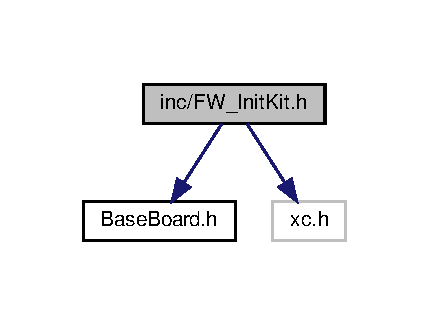
\includegraphics[width=206pt]{d9/dc6/FW__InitKit_8h__incl}
\end{center}
\end{figure}
Gráfico de los archivos que directa o indirectamente incluyen a este archivo\+:\nopagebreak
\begin{figure}[H]
\begin{center}
\leavevmode
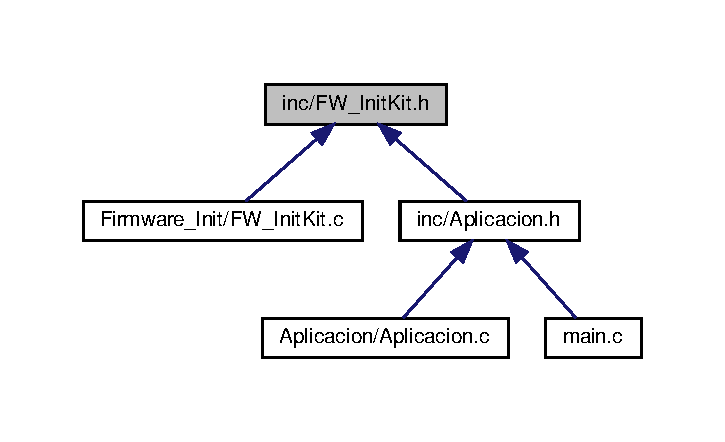
\includegraphics[width=348pt]{d5/d7d/FW__InitKit_8h__dep__incl}
\end{center}
\end{figure}
\subsection*{Funciones}
\begin{DoxyCompactItemize}
\item 
void \hyperlink{FW__InitKit_8h_a91a9e93581be29c6af058d09741ee5be}{Kit\+\_\+\+Init} (void)
\begin{DoxyCompactList}\small\item\em Inicializa el entrenador para el shield 1. \end{DoxyCompactList}\end{DoxyCompactItemize}


\subsection{Documentación de las funciones}
\mbox{\Hypertarget{FW__InitKit_8h_a91a9e93581be29c6af058d09741ee5be}\label{FW__InitKit_8h_a91a9e93581be29c6af058d09741ee5be}} 
\index{F\+W\+\_\+\+Init\+Kit.\+h@{F\+W\+\_\+\+Init\+Kit.\+h}!Kit\+\_\+\+Init@{Kit\+\_\+\+Init}}
\index{Kit\+\_\+\+Init@{Kit\+\_\+\+Init}!F\+W\+\_\+\+Init\+Kit.\+h@{F\+W\+\_\+\+Init\+Kit.\+h}}
\subsubsection{\texorpdfstring{Kit\+\_\+\+Init()}{Kit\_Init()}}
{\footnotesize\ttfamily void Kit\+\_\+\+Init (\begin{DoxyParamCaption}\item[{void}]{ }\end{DoxyParamCaption})}



Inicializa el entrenador para el shield 1. 

Inicializa todos los puertos del entrenador preparandolo para usar el display y deshabilitando los comparadores de entrada y los canales anal�gicos. Tambi�n limpia todas las salidas. \begin{DoxyAuthor}{Autor}
Esteban Lemos 
\end{DoxyAuthor}
\begin{DoxyDate}{Fecha}

\end{DoxyDate}

\begin{DoxyParams}[1]{Parámetros}
\mbox{\tt in}  & {\em void} & \\
\hline
\mbox{\tt out}  & {\em void} & \\
\hline
\end{DoxyParams}
\begin{DoxyReturn}{Devuelve}
void 
\end{DoxyReturn}


Definición en la línea 65 del archivo F\+W\+\_\+\+Init\+Kit.\+c.

Gráfico de llamadas a esta función\+:\nopagebreak
\begin{figure}[H]
\begin{center}
\leavevmode
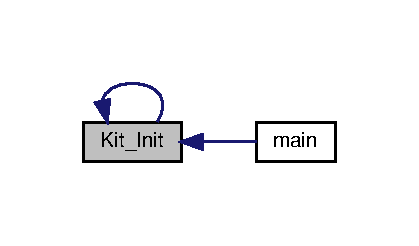
\includegraphics[width=201pt]{d5/dee/FW__InitKit_8h_a91a9e93581be29c6af058d09741ee5be_icgraph}
\end{center}
\end{figure}

\hypertarget{FW__InitTimer_8h}{}\section{Referencia del Archivo inc/\+F\+W\+\_\+\+Init\+Timer.h}
\label{FW__InitTimer_8h}\index{inc/\+F\+W\+\_\+\+Init\+Timer.\+h@{inc/\+F\+W\+\_\+\+Init\+Timer.\+h}}
{\ttfamily \#include $<$xc.\+h$>$}\newline
Dependencia gráfica adjunta para F\+W\+\_\+\+Init\+Timer.\+h\+:\nopagebreak
\begin{figure}[H]
\begin{center}
\leavevmode
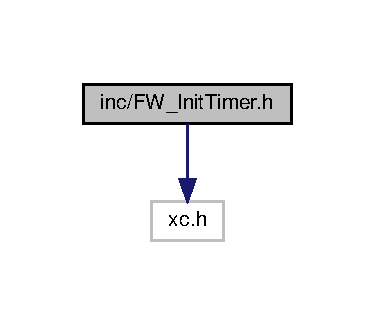
\includegraphics[width=180pt]{da/d12/FW__InitTimer_8h__incl}
\end{center}
\end{figure}
Gráfico de los archivos que directa o indirectamente incluyen a este archivo\+:\nopagebreak
\begin{figure}[H]
\begin{center}
\leavevmode
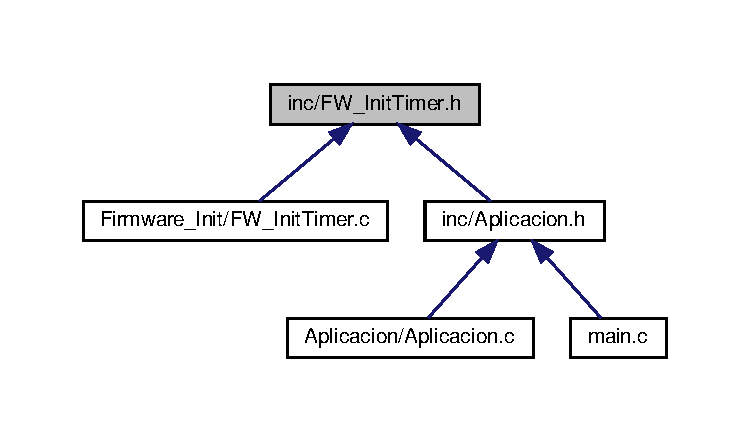
\includegraphics[width=350pt]{d0/d6f/FW__InitTimer_8h__dep__incl}
\end{center}
\end{figure}
\subsection*{Funciones}
\begin{DoxyCompactItemize}
\item 
void \hyperlink{FW__InitTimer_8h_abd382c7fbfb96997eaf343338a95fba1}{Tmr0\+\_\+\+Init} (void)
\begin{DoxyCompactList}\small\item\em Inicializacion del Tmr0. \end{DoxyCompactList}\item 
void \hyperlink{FW__InitTimer_8h_a43979f9e4c8e7a7d91c40ab087b4e312}{Tmr1\+\_\+\+Init} (void)
\begin{DoxyCompactList}\small\item\em Inicializacion del Tmr1. \end{DoxyCompactList}\end{DoxyCompactItemize}


\subsection{Documentación de las funciones}
\mbox{\Hypertarget{FW__InitTimer_8h_abd382c7fbfb96997eaf343338a95fba1}\label{FW__InitTimer_8h_abd382c7fbfb96997eaf343338a95fba1}} 
\index{F\+W\+\_\+\+Init\+Timer.\+h@{F\+W\+\_\+\+Init\+Timer.\+h}!Tmr0\+\_\+\+Init@{Tmr0\+\_\+\+Init}}
\index{Tmr0\+\_\+\+Init@{Tmr0\+\_\+\+Init}!F\+W\+\_\+\+Init\+Timer.\+h@{F\+W\+\_\+\+Init\+Timer.\+h}}
\subsubsection{\texorpdfstring{Tmr0\+\_\+\+Init()}{Tmr0\_Init()}}
{\footnotesize\ttfamily void Tmr0\+\_\+\+Init (\begin{DoxyParamCaption}\item[{void}]{ }\end{DoxyParamCaption})}



Inicializacion del Tmr0. 

Inicializa el timer 0 en 8 bits, con el prescaler en 256 y con la interrupcion activada. Esta configurado para que interrumpa cada 1.\+0022ms \begin{DoxyAuthor}{Autor}
I Esteban Lemos 
\end{DoxyAuthor}
\begin{DoxyDate}{Fecha}

\end{DoxyDate}

\begin{DoxyParams}[1]{Parámetros}
\mbox{\tt in}  & {\em void} & \\
\hline
\mbox{\tt out}  & {\em void} & \\
\hline
\end{DoxyParams}
\begin{DoxyReturn}{Devuelve}
void 
\end{DoxyReturn}


Definición en la línea 67 del archivo F\+W\+\_\+\+Init\+Timer.\+c.

Gráfico de llamadas a esta función\+:\nopagebreak
\begin{figure}[H]
\begin{center}
\leavevmode
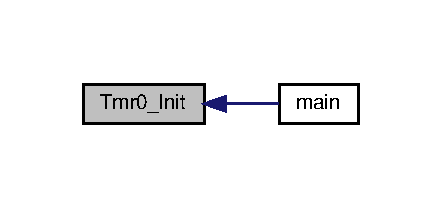
\includegraphics[width=212pt]{da/d62/FW__InitTimer_8h_abd382c7fbfb96997eaf343338a95fba1_icgraph}
\end{center}
\end{figure}
\mbox{\Hypertarget{FW__InitTimer_8h_a43979f9e4c8e7a7d91c40ab087b4e312}\label{FW__InitTimer_8h_a43979f9e4c8e7a7d91c40ab087b4e312}} 
\index{F\+W\+\_\+\+Init\+Timer.\+h@{F\+W\+\_\+\+Init\+Timer.\+h}!Tmr1\+\_\+\+Init@{Tmr1\+\_\+\+Init}}
\index{Tmr1\+\_\+\+Init@{Tmr1\+\_\+\+Init}!F\+W\+\_\+\+Init\+Timer.\+h@{F\+W\+\_\+\+Init\+Timer.\+h}}
\subsubsection{\texorpdfstring{Tmr1\+\_\+\+Init()}{Tmr1\_Init()}}
{\footnotesize\ttfamily void Tmr1\+\_\+\+Init (\begin{DoxyParamCaption}\item[{void}]{ }\end{DoxyParamCaption})}



Inicializacion del Tmr1. 

Inicializa el timer 0 en 8 bits, con el prescaler en 256 y con la interrupcion activada. Esta configurado para que interrumpa cada 99,96 uS \begin{DoxyAuthor}{Autor}
I Esteban Lemos 
\end{DoxyAuthor}
\begin{DoxyDate}{Fecha}

\end{DoxyDate}

\begin{DoxyParams}[1]{Parámetros}
\mbox{\tt in}  & {\em void} & \\
\hline
\mbox{\tt out}  & {\em void} & \\
\hline
\end{DoxyParams}
\begin{DoxyReturn}{Devuelve}
void 
\end{DoxyReturn}


Definición en la línea 94 del archivo F\+W\+\_\+\+Init\+Timer.\+c.


\hypertarget{FW__LCD_8h}{}\section{Referencia del Archivo inc/\+F\+W\+\_\+\+L\+CD.h}
\label{FW__LCD_8h}\index{inc/\+F\+W\+\_\+\+L\+C\+D.\+h@{inc/\+F\+W\+\_\+\+L\+C\+D.\+h}}
{\ttfamily \#include $<$xc.\+h$>$}\newline
{\ttfamily \#include \char`\"{}P\+R\+\_\+\+L\+C\+D.\+h\char`\"{}}\newline
{\ttfamily \#include \char`\"{}Base\+Board.\+h\char`\"{}}\newline
Dependencia gráfica adjunta para F\+W\+\_\+\+L\+C\+D.\+h\+:\nopagebreak
\begin{figure}[H]
\begin{center}
\leavevmode
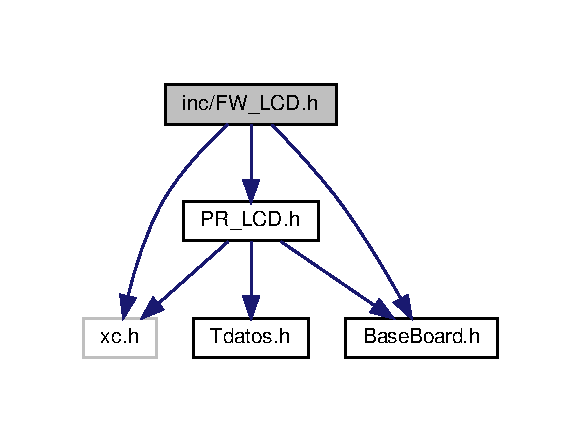
\includegraphics[width=279pt]{d9/df6/FW__LCD_8h__incl}
\end{center}
\end{figure}
Gráfico de los archivos que directa o indirectamente incluyen a este archivo\+:\nopagebreak
\begin{figure}[H]
\begin{center}
\leavevmode
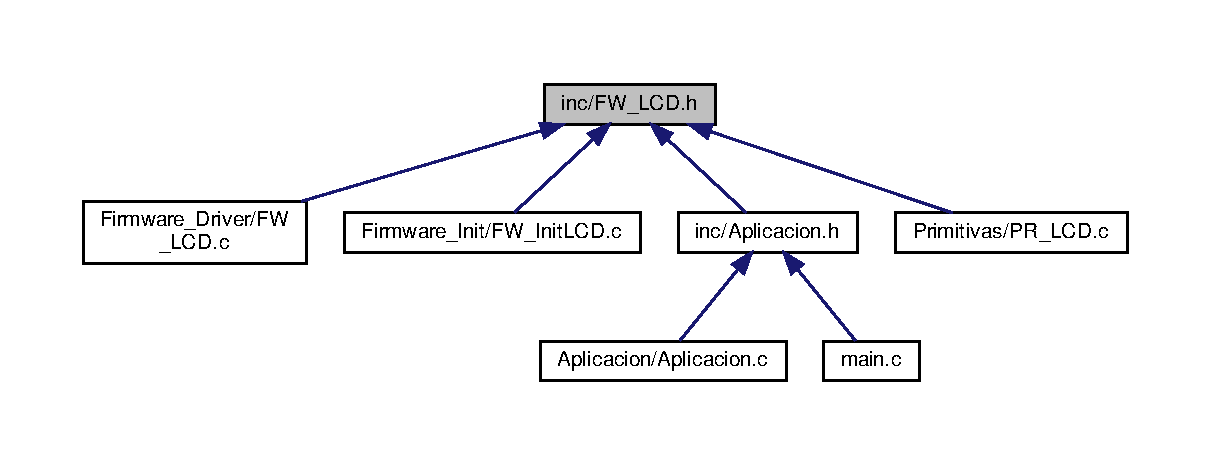
\includegraphics[width=350pt]{d4/da9/FW__LCD_8h__dep__incl}
\end{center}
\end{figure}

\hypertarget{FW__Teclado_8h}{}\section{Referencia del Archivo inc/\+F\+W\+\_\+\+Teclado.h}
\label{FW__Teclado_8h}\index{inc/\+F\+W\+\_\+\+Teclado.\+h@{inc/\+F\+W\+\_\+\+Teclado.\+h}}
{\ttfamily \#include $<$xc.\+h$>$}\newline
{\ttfamily \#include \char`\"{}Tdatos.\+h\char`\"{}}\newline
{\ttfamily \#include \char`\"{}P\+R\+\_\+\+Teclado.\+h\char`\"{}}\newline
{\ttfamily \#include \char`\"{}Base\+Board.\+h\char`\"{}}\newline
Dependencia gráfica adjunta para F\+W\+\_\+\+Teclado.\+h\+:\nopagebreak
\begin{figure}[H]
\begin{center}
\leavevmode
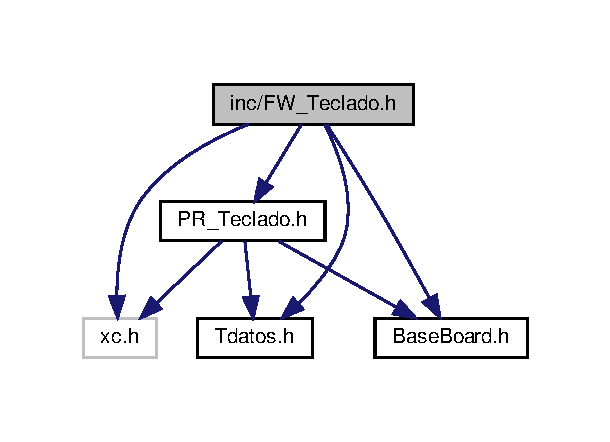
\includegraphics[width=293pt]{d5/db7/FW__Teclado_8h__incl}
\end{center}
\end{figure}
Gráfico de los archivos que directa o indirectamente incluyen a este archivo\+:\nopagebreak
\begin{figure}[H]
\begin{center}
\leavevmode
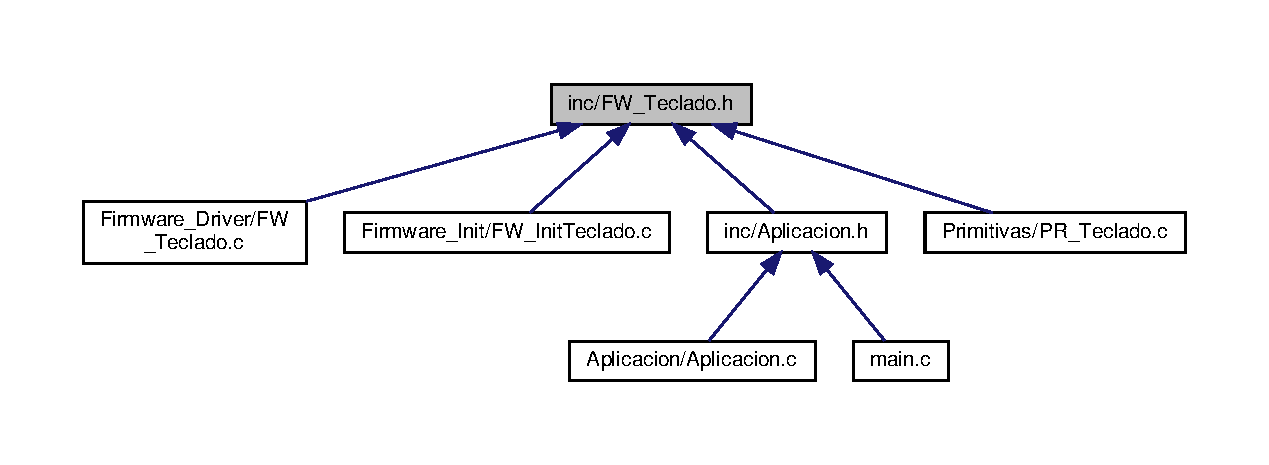
\includegraphics[width=350pt]{d2/df7/FW__Teclado_8h__dep__incl}
\end{center}
\end{figure}
\subsection*{Funciones}
\begin{DoxyCompactItemize}
\item 
void \hyperlink{FW__Teclado_8h_afca05d832c45a47fe754f4ab43de364e}{T\+D\+O\+\_\+\+Init} (void)
\begin{DoxyCompactList}\small\item\em Inicializa el puerto y las interrupciones. \end{DoxyCompactList}\item 
void \hyperlink{FW__Teclado_8h_a64caa519224486b8d93e72a92156679a}{T\+D\+O\+\_\+\+Marca\+Tecla} (void)
\item 
void \hyperlink{FW__Teclado_8h_a0baf84f98398f0ba3fa364fec157e136}{T\+D\+O\+\_\+\+Tic} (void)
\item 
void \hyperlink{FW__Teclado_8h_a72699b8ff8dd75ac13b3fc778bfe365e}{T\+D\+O\+\_\+\+Little\+Delay} (void)
\begin{DoxyCompactList}\small\item\em demora breve \end{DoxyCompactList}\end{DoxyCompactItemize}


\subsection{Documentación de las funciones}
\mbox{\Hypertarget{FW__Teclado_8h_afca05d832c45a47fe754f4ab43de364e}\label{FW__Teclado_8h_afca05d832c45a47fe754f4ab43de364e}} 
\index{F\+W\+\_\+\+Teclado.\+h@{F\+W\+\_\+\+Teclado.\+h}!T\+D\+O\+\_\+\+Init@{T\+D\+O\+\_\+\+Init}}
\index{T\+D\+O\+\_\+\+Init@{T\+D\+O\+\_\+\+Init}!F\+W\+\_\+\+Teclado.\+h@{F\+W\+\_\+\+Teclado.\+h}}
\subsubsection{\texorpdfstring{T\+D\+O\+\_\+\+Init()}{TDO\_Init()}}
{\footnotesize\ttfamily void T\+D\+O\+\_\+\+Init (\begin{DoxyParamCaption}\item[{void}]{ }\end{DoxyParamCaption})}



Inicializa el puerto y las interrupciones. 

La siguiente funcion inicializa el puerto y las interrupciones. $\ast$ Para incorporar el teclado al puerto B debe de llamarse luego de\+: $\ast$ \hyperlink{FW__InitKit_8c_a91a9e93581be29c6af058d09741ee5be}{Kit\+\_\+\+Init()} y \hyperlink{FW__InitTimer_8c_a4d368e642dbd363e361c8be19cd144eb}{Tmr0\+\_\+\+Init()} I\+M\+P\+O\+R\+T\+A\+N\+T\+E!! esta funci�n solamente funciona con el Shield 1.\+3 y no debe de ser tenida en cuenta para otros micros o placas \begin{DoxyAuthor}{Autor}
Esteban Lemos 
\end{DoxyAuthor}
\begin{DoxyDate}{Fecha}

\end{DoxyDate}


Definición en la línea 94 del archivo F\+W\+\_\+\+Init\+Teclado.\+c.

\mbox{\Hypertarget{FW__Teclado_8h_a72699b8ff8dd75ac13b3fc778bfe365e}\label{FW__Teclado_8h_a72699b8ff8dd75ac13b3fc778bfe365e}} 
\index{F\+W\+\_\+\+Teclado.\+h@{F\+W\+\_\+\+Teclado.\+h}!T\+D\+O\+\_\+\+Little\+Delay@{T\+D\+O\+\_\+\+Little\+Delay}}
\index{T\+D\+O\+\_\+\+Little\+Delay@{T\+D\+O\+\_\+\+Little\+Delay}!F\+W\+\_\+\+Teclado.\+h@{F\+W\+\_\+\+Teclado.\+h}}
\subsubsection{\texorpdfstring{T\+D\+O\+\_\+\+Little\+Delay()}{TDO\_LittleDelay()}}
{\footnotesize\ttfamily void T\+D\+O\+\_\+\+Little\+Delay (\begin{DoxyParamCaption}\item[{void}]{ }\end{DoxyParamCaption})}



demora breve 

\begin{DoxyAuthor}{Autor}
Esteban Lemos 
\end{DoxyAuthor}
\begin{DoxyDate}{Fecha}

\end{DoxyDate}


Definición en la línea 120 del archivo F\+W\+\_\+\+Teclado.\+c.

Gráfico de llamadas a esta función\+:\nopagebreak
\begin{figure}[H]
\begin{center}
\leavevmode
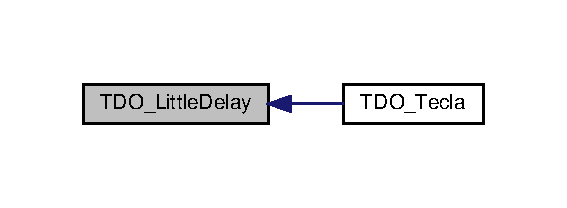
\includegraphics[width=272pt]{df/d5a/FW__Teclado_8h_a72699b8ff8dd75ac13b3fc778bfe365e_icgraph}
\end{center}
\end{figure}
\mbox{\Hypertarget{FW__Teclado_8h_a64caa519224486b8d93e72a92156679a}\label{FW__Teclado_8h_a64caa519224486b8d93e72a92156679a}} 
\index{F\+W\+\_\+\+Teclado.\+h@{F\+W\+\_\+\+Teclado.\+h}!T\+D\+O\+\_\+\+Marca\+Tecla@{T\+D\+O\+\_\+\+Marca\+Tecla}}
\index{T\+D\+O\+\_\+\+Marca\+Tecla@{T\+D\+O\+\_\+\+Marca\+Tecla}!F\+W\+\_\+\+Teclado.\+h@{F\+W\+\_\+\+Teclado.\+h}}
\subsubsection{\texorpdfstring{T\+D\+O\+\_\+\+Marca\+Tecla()}{TDO\_MarcaTecla()}}
{\footnotesize\ttfamily void T\+D\+O\+\_\+\+Marca\+Tecla (\begin{DoxyParamCaption}\item[{void}]{ }\end{DoxyParamCaption})}

Funcion para uso de teclado la misma se incluye en la interrupci�n de teclado. La misma pone un estado alto el flag que indica el evento de teclado para otros micros o placas \begin{DoxyAuthor}{Autor}
Esteban Lemos 
\end{DoxyAuthor}
\begin{DoxyDate}{Fecha}

\end{DoxyDate}


Definición en la línea 90 del archivo F\+W\+\_\+\+Teclado.\+c.

\mbox{\Hypertarget{FW__Teclado_8h_a0baf84f98398f0ba3fa364fec157e136}\label{FW__Teclado_8h_a0baf84f98398f0ba3fa364fec157e136}} 
\index{F\+W\+\_\+\+Teclado.\+h@{F\+W\+\_\+\+Teclado.\+h}!T\+D\+O\+\_\+\+Tic@{T\+D\+O\+\_\+\+Tic}}
\index{T\+D\+O\+\_\+\+Tic@{T\+D\+O\+\_\+\+Tic}!F\+W\+\_\+\+Teclado.\+h@{F\+W\+\_\+\+Teclado.\+h}}
\subsubsection{\texorpdfstring{T\+D\+O\+\_\+\+Tic()}{TDO\_Tic()}}
{\footnotesize\ttfamily void T\+D\+O\+\_\+\+Tic (\begin{DoxyParamCaption}\item[{void}]{ }\end{DoxyParamCaption})}

Funci�n para el tratamiento del rebote se incluye en la interrupci�n del timer , que deber� estar configurado en 1ms un milisegundo. La misma decrementa una variable que se encarga de definir los tiempos de estabilidad y as� evitar el rebote. \begin{DoxyAuthor}{Autor}
Esteban Lemos 
\end{DoxyAuthor}
\begin{DoxyDate}{Fecha}

\end{DoxyDate}


Definición en la línea 109 del archivo F\+W\+\_\+\+Teclado.\+c.


\hypertarget{MacTimer_8h}{}\section{Referencia del Archivo inc/\+Mac\+Timer.h}
\label{MacTimer_8h}\index{inc/\+Mac\+Timer.\+h@{inc/\+Mac\+Timer.\+h}}
{\ttfamily \#include \char`\"{}Tdatos.\+h\char`\"{}}\newline
Dependencia gráfica adjunta para Mac\+Timer.\+h\+:\nopagebreak
\begin{figure}[H]
\begin{center}
\leavevmode
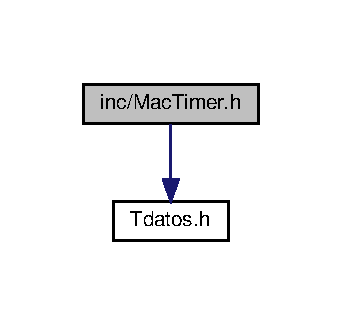
\includegraphics[width=164pt]{d4/db4/MacTimer_8h__incl}
\end{center}
\end{figure}
Gráfico de los archivos que directa o indirectamente incluyen a este archivo\+:\nopagebreak
\begin{figure}[H]
\begin{center}
\leavevmode
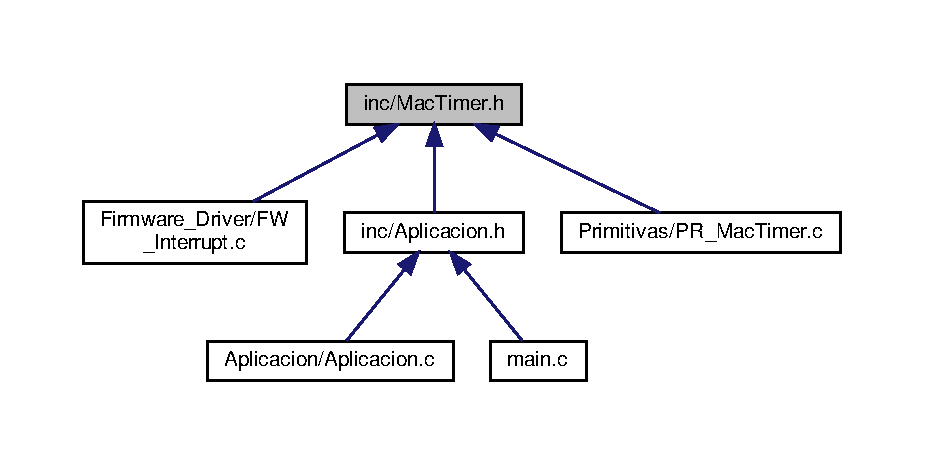
\includegraphics[width=350pt]{d0/d81/MacTimer_8h__dep__incl}
\end{center}
\end{figure}
\subsection*{defines}
\begin{DoxyCompactItemize}
\item 
\#define \hyperlink{MacTimer_8h_a81bf35758ad812f44a7e314120a2ec7e}{M\+C\+T\+M\+R\+\_\+\+T\+I\+M\+E\+RS}~8
\item 
\#define \hyperlink{MacTimer_8h_ac3fd3d1eece17e26cf87b8316fe3c4d3}{M\+C\+T\+M\+R\+\_\+\+E\+V\+E\+N\+T\+O0}~0
\item 
\#define \hyperlink{MacTimer_8h_adf23caca1af9924cf0a865cceab3d986}{M\+C\+T\+M\+R\+\_\+\+E\+V\+E\+N\+T\+O1}~1
\item 
\#define \hyperlink{MacTimer_8h_ae0eaaf15120e3159dcdaa437433dcc6f}{M\+C\+T\+M\+R\+\_\+\+E\+V\+E\+N\+T\+O2}~2
\item 
\#define \hyperlink{MacTimer_8h_ab2fceb9cb3d0424ad8cd5f8c7ee46e3a}{M\+C\+T\+M\+R\+\_\+\+E\+V\+E\+N\+T\+O3}~3
\item 
\#define \hyperlink{MacTimer_8h_a8a009da3ccc23468ec2adcf1c2d1c7f1}{M\+C\+T\+M\+R\+\_\+\+E\+V\+E\+N\+T\+O4}~4
\item 
\#define \hyperlink{MacTimer_8h_a0109bfb6b9337c8b5411c6e46fc4a3f9}{M\+C\+T\+M\+R\+\_\+\+E\+V\+E\+N\+T\+O5}~5
\item 
\#define \hyperlink{MacTimer_8h_a8e606e8bc0605d66dcb6626fe9746b54}{M\+C\+T\+M\+R\+\_\+\+E\+V\+E\+N\+T\+O6}~6
\item 
\#define \hyperlink{MacTimer_8h_a34e375fabbfa6575c55994a1868d85d2}{M\+C\+T\+M\+R\+\_\+\+E\+V\+E\+N\+T\+O7}~7
\item 
\#define \hyperlink{MacTimer_8h_a27d0b76cf849ca6c4eb279c34efa8e0c}{M\+C\+T\+M\+R\+\_\+\+T0}~1000
\item 
\#define \hyperlink{MacTimer_8h_ac6effe9877e54bb593c341872621c463}{M\+C\+T\+M\+R\+\_\+\+T1}~2000
\item 
\#define \hyperlink{MacTimer_8h_a1a850d6bb798f1dfdaf63c40151d0512}{M\+C\+T\+M\+R\+\_\+\+T2}~3000
\item 
\#define \hyperlink{MacTimer_8h_abbda59f7b1a2a13a70934b868c520e08}{M\+C\+T\+M\+R\+\_\+\+T3}~4000
\item 
\#define \hyperlink{MacTimer_8h_aa690aa98b442f8949aa4bf6a505d0a7d}{M\+C\+T\+M\+R\+\_\+\+T4}~5000
\item 
\#define \hyperlink{MacTimer_8h_a492ecf19e5cc6e72dae299fe58e49797}{M\+C\+T\+M\+R\+\_\+\+T5}~6000
\item 
\#define \hyperlink{MacTimer_8h_a61418a5f98ecf5d506ca580da674ec53}{M\+C\+T\+M\+R\+\_\+\+T6}~7000
\item 
\#define \hyperlink{MacTimer_8h_a2a3b21479493e6243d9cb4ba388c9f46}{M\+C\+T\+M\+R\+\_\+\+T7}~8000
\item 
\#define \hyperlink{MacTimer_8h_ab80f39f4c525b385e4f82c41484b4b96}{M\+C\+T\+M\+R\+\_\+\+L\+I\+M\+P\+I\+O\+\_\+\+B\+A\+N\+D\+E\+RA}~\hyperlink{PR__MacTimer_8c_a5eb4db3b88aa80a93fea88c732624601}{M\+C\+T\+M\+R\+\_\+\+Eventos} \&= $\sim$i
\end{DoxyCompactItemize}
\subsection*{Funciones}
\begin{DoxyCompactItemize}
\item 
void \hyperlink{MacTimer_8h_a4c8b1a8d2adf9edcefa637611ede4c37}{M\+C\+T\+M\+R\+\_\+\+Analizar} (void)
\begin{DoxyCompactList}\small\item\em Descuento de Timers. No es una primitiva. Es una funci�n de la capa inferior. La ubico en este .c para tener todas las funciones de timers juntas. \end{DoxyCompactList}\item 
void \hyperlink{MacTimer_8h_a4fb7b92a9ec9798ba7231409dc5952bc}{M\+C\+T\+M\+R\+\_\+\+Start} (\hyperlink{Tdatos_8h_aba7bc1797add20fe3efdf37ced1182c5}{uint8\+\_\+t} evento, \hyperlink{Tdatos_8h_aba7bc1797add20fe3efdf37ced1182c5}{uint8\+\_\+t} temp)
\begin{DoxyCompactList}\small\item\em Lanzamientos de Timers. \end{DoxyCompactList}\item 
void \hyperlink{MacTimer_8h_a3c2851c33967c1e1e7100cc8d0f49e94}{M\+C\+T\+M\+R\+\_\+\+Stop} (\hyperlink{Tdatos_8h_aba7bc1797add20fe3efdf37ced1182c5}{uint8\+\_\+t} evento)
\begin{DoxyCompactList}\small\item\em Aapaga el timer indicado. \end{DoxyCompactList}\item 
void \hyperlink{MacTimer_8h_a48debe9df780acf2b014e64bc15fa20c}{M\+C\+T\+M\+R\+\_\+\+Close} (void)
\begin{DoxyCompactList}\small\item\em Apaga todo los timers. \end{DoxyCompactList}\item 
void \hyperlink{MacTimer_8h_a676be584825c2eda6c4dd5fb57ff4acb}{M\+C\+T\+M\+R\+\_\+\+Event} (void)
\begin{DoxyCompactList}\small\item\em Analiza Eventos de timers. No es una primitiva. Es parte o toda la aplicaci�n La ubico en este .c para tener todas las funciones de timers juntas. \end{DoxyCompactList}\end{DoxyCompactItemize}
\subsection*{Variables}
\begin{DoxyCompactItemize}
\item 
volatile \hyperlink{Tdatos_8h_adf4d876453337156dde61095e1f20223}{uint16\+\_\+t} \hyperlink{MacTimer_8h_a8b428db727bdc812d532f747cec0c004}{M\+C\+T\+M\+R\+\_\+\+Run} \mbox{[}\hyperlink{MacTimer_8h_a81bf35758ad812f44a7e314120a2ec7e}{M\+C\+T\+M\+R\+\_\+\+T\+I\+M\+E\+RS}\mbox{]}
\begin{DoxyCompactList}\small\item\em el tipo de dato lo defino dependiendo el timepo que \end{DoxyCompactList}\item 
volatile \hyperlink{Tdatos_8h_aba7bc1797add20fe3efdf37ced1182c5}{uint8\+\_\+t} \hyperlink{MacTimer_8h_a5eb4db3b88aa80a93fea88c732624601}{M\+C\+T\+M\+R\+\_\+\+Eventos}
\begin{DoxyCompactList}\small\item\em necesite y la base de tiempo propuesta cada posic�n \end{DoxyCompactList}\end{DoxyCompactItemize}


\subsection{Documentación de los \textquotesingle{}defines\textquotesingle{}}
\mbox{\Hypertarget{MacTimer_8h_ac3fd3d1eece17e26cf87b8316fe3c4d3}\label{MacTimer_8h_ac3fd3d1eece17e26cf87b8316fe3c4d3}} 
\index{Mac\+Timer.\+h@{Mac\+Timer.\+h}!M\+C\+T\+M\+R\+\_\+\+E\+V\+E\+N\+T\+O0@{M\+C\+T\+M\+R\+\_\+\+E\+V\+E\+N\+T\+O0}}
\index{M\+C\+T\+M\+R\+\_\+\+E\+V\+E\+N\+T\+O0@{M\+C\+T\+M\+R\+\_\+\+E\+V\+E\+N\+T\+O0}!Mac\+Timer.\+h@{Mac\+Timer.\+h}}
\subsubsection{\texorpdfstring{M\+C\+T\+M\+R\+\_\+\+E\+V\+E\+N\+T\+O0}{MCTMR\_EVENTO0}}
{\footnotesize\ttfamily \#define M\+C\+T\+M\+R\+\_\+\+E\+V\+E\+N\+T\+O0~0}



Definición en la línea 64 del archivo Mac\+Timer.\+h.

\mbox{\Hypertarget{MacTimer_8h_adf23caca1af9924cf0a865cceab3d986}\label{MacTimer_8h_adf23caca1af9924cf0a865cceab3d986}} 
\index{Mac\+Timer.\+h@{Mac\+Timer.\+h}!M\+C\+T\+M\+R\+\_\+\+E\+V\+E\+N\+T\+O1@{M\+C\+T\+M\+R\+\_\+\+E\+V\+E\+N\+T\+O1}}
\index{M\+C\+T\+M\+R\+\_\+\+E\+V\+E\+N\+T\+O1@{M\+C\+T\+M\+R\+\_\+\+E\+V\+E\+N\+T\+O1}!Mac\+Timer.\+h@{Mac\+Timer.\+h}}
\subsubsection{\texorpdfstring{M\+C\+T\+M\+R\+\_\+\+E\+V\+E\+N\+T\+O1}{MCTMR\_EVENTO1}}
{\footnotesize\ttfamily \#define M\+C\+T\+M\+R\+\_\+\+E\+V\+E\+N\+T\+O1~1}



Definición en la línea 65 del archivo Mac\+Timer.\+h.

\mbox{\Hypertarget{MacTimer_8h_ae0eaaf15120e3159dcdaa437433dcc6f}\label{MacTimer_8h_ae0eaaf15120e3159dcdaa437433dcc6f}} 
\index{Mac\+Timer.\+h@{Mac\+Timer.\+h}!M\+C\+T\+M\+R\+\_\+\+E\+V\+E\+N\+T\+O2@{M\+C\+T\+M\+R\+\_\+\+E\+V\+E\+N\+T\+O2}}
\index{M\+C\+T\+M\+R\+\_\+\+E\+V\+E\+N\+T\+O2@{M\+C\+T\+M\+R\+\_\+\+E\+V\+E\+N\+T\+O2}!Mac\+Timer.\+h@{Mac\+Timer.\+h}}
\subsubsection{\texorpdfstring{M\+C\+T\+M\+R\+\_\+\+E\+V\+E\+N\+T\+O2}{MCTMR\_EVENTO2}}
{\footnotesize\ttfamily \#define M\+C\+T\+M\+R\+\_\+\+E\+V\+E\+N\+T\+O2~2}



Definición en la línea 66 del archivo Mac\+Timer.\+h.

\mbox{\Hypertarget{MacTimer_8h_ab2fceb9cb3d0424ad8cd5f8c7ee46e3a}\label{MacTimer_8h_ab2fceb9cb3d0424ad8cd5f8c7ee46e3a}} 
\index{Mac\+Timer.\+h@{Mac\+Timer.\+h}!M\+C\+T\+M\+R\+\_\+\+E\+V\+E\+N\+T\+O3@{M\+C\+T\+M\+R\+\_\+\+E\+V\+E\+N\+T\+O3}}
\index{M\+C\+T\+M\+R\+\_\+\+E\+V\+E\+N\+T\+O3@{M\+C\+T\+M\+R\+\_\+\+E\+V\+E\+N\+T\+O3}!Mac\+Timer.\+h@{Mac\+Timer.\+h}}
\subsubsection{\texorpdfstring{M\+C\+T\+M\+R\+\_\+\+E\+V\+E\+N\+T\+O3}{MCTMR\_EVENTO3}}
{\footnotesize\ttfamily \#define M\+C\+T\+M\+R\+\_\+\+E\+V\+E\+N\+T\+O3~3}



Definición en la línea 67 del archivo Mac\+Timer.\+h.

\mbox{\Hypertarget{MacTimer_8h_a8a009da3ccc23468ec2adcf1c2d1c7f1}\label{MacTimer_8h_a8a009da3ccc23468ec2adcf1c2d1c7f1}} 
\index{Mac\+Timer.\+h@{Mac\+Timer.\+h}!M\+C\+T\+M\+R\+\_\+\+E\+V\+E\+N\+T\+O4@{M\+C\+T\+M\+R\+\_\+\+E\+V\+E\+N\+T\+O4}}
\index{M\+C\+T\+M\+R\+\_\+\+E\+V\+E\+N\+T\+O4@{M\+C\+T\+M\+R\+\_\+\+E\+V\+E\+N\+T\+O4}!Mac\+Timer.\+h@{Mac\+Timer.\+h}}
\subsubsection{\texorpdfstring{M\+C\+T\+M\+R\+\_\+\+E\+V\+E\+N\+T\+O4}{MCTMR\_EVENTO4}}
{\footnotesize\ttfamily \#define M\+C\+T\+M\+R\+\_\+\+E\+V\+E\+N\+T\+O4~4}



Definición en la línea 68 del archivo Mac\+Timer.\+h.

\mbox{\Hypertarget{MacTimer_8h_a0109bfb6b9337c8b5411c6e46fc4a3f9}\label{MacTimer_8h_a0109bfb6b9337c8b5411c6e46fc4a3f9}} 
\index{Mac\+Timer.\+h@{Mac\+Timer.\+h}!M\+C\+T\+M\+R\+\_\+\+E\+V\+E\+N\+T\+O5@{M\+C\+T\+M\+R\+\_\+\+E\+V\+E\+N\+T\+O5}}
\index{M\+C\+T\+M\+R\+\_\+\+E\+V\+E\+N\+T\+O5@{M\+C\+T\+M\+R\+\_\+\+E\+V\+E\+N\+T\+O5}!Mac\+Timer.\+h@{Mac\+Timer.\+h}}
\subsubsection{\texorpdfstring{M\+C\+T\+M\+R\+\_\+\+E\+V\+E\+N\+T\+O5}{MCTMR\_EVENTO5}}
{\footnotesize\ttfamily \#define M\+C\+T\+M\+R\+\_\+\+E\+V\+E\+N\+T\+O5~5}



Definición en la línea 69 del archivo Mac\+Timer.\+h.

\mbox{\Hypertarget{MacTimer_8h_a8e606e8bc0605d66dcb6626fe9746b54}\label{MacTimer_8h_a8e606e8bc0605d66dcb6626fe9746b54}} 
\index{Mac\+Timer.\+h@{Mac\+Timer.\+h}!M\+C\+T\+M\+R\+\_\+\+E\+V\+E\+N\+T\+O6@{M\+C\+T\+M\+R\+\_\+\+E\+V\+E\+N\+T\+O6}}
\index{M\+C\+T\+M\+R\+\_\+\+E\+V\+E\+N\+T\+O6@{M\+C\+T\+M\+R\+\_\+\+E\+V\+E\+N\+T\+O6}!Mac\+Timer.\+h@{Mac\+Timer.\+h}}
\subsubsection{\texorpdfstring{M\+C\+T\+M\+R\+\_\+\+E\+V\+E\+N\+T\+O6}{MCTMR\_EVENTO6}}
{\footnotesize\ttfamily \#define M\+C\+T\+M\+R\+\_\+\+E\+V\+E\+N\+T\+O6~6}



Definición en la línea 70 del archivo Mac\+Timer.\+h.

\mbox{\Hypertarget{MacTimer_8h_a34e375fabbfa6575c55994a1868d85d2}\label{MacTimer_8h_a34e375fabbfa6575c55994a1868d85d2}} 
\index{Mac\+Timer.\+h@{Mac\+Timer.\+h}!M\+C\+T\+M\+R\+\_\+\+E\+V\+E\+N\+T\+O7@{M\+C\+T\+M\+R\+\_\+\+E\+V\+E\+N\+T\+O7}}
\index{M\+C\+T\+M\+R\+\_\+\+E\+V\+E\+N\+T\+O7@{M\+C\+T\+M\+R\+\_\+\+E\+V\+E\+N\+T\+O7}!Mac\+Timer.\+h@{Mac\+Timer.\+h}}
\subsubsection{\texorpdfstring{M\+C\+T\+M\+R\+\_\+\+E\+V\+E\+N\+T\+O7}{MCTMR\_EVENTO7}}
{\footnotesize\ttfamily \#define M\+C\+T\+M\+R\+\_\+\+E\+V\+E\+N\+T\+O7~7}



Definición en la línea 71 del archivo Mac\+Timer.\+h.

\mbox{\Hypertarget{MacTimer_8h_ab80f39f4c525b385e4f82c41484b4b96}\label{MacTimer_8h_ab80f39f4c525b385e4f82c41484b4b96}} 
\index{Mac\+Timer.\+h@{Mac\+Timer.\+h}!M\+C\+T\+M\+R\+\_\+\+L\+I\+M\+P\+I\+O\+\_\+\+B\+A\+N\+D\+E\+RA@{M\+C\+T\+M\+R\+\_\+\+L\+I\+M\+P\+I\+O\+\_\+\+B\+A\+N\+D\+E\+RA}}
\index{M\+C\+T\+M\+R\+\_\+\+L\+I\+M\+P\+I\+O\+\_\+\+B\+A\+N\+D\+E\+RA@{M\+C\+T\+M\+R\+\_\+\+L\+I\+M\+P\+I\+O\+\_\+\+B\+A\+N\+D\+E\+RA}!Mac\+Timer.\+h@{Mac\+Timer.\+h}}
\subsubsection{\texorpdfstring{M\+C\+T\+M\+R\+\_\+\+L\+I\+M\+P\+I\+O\+\_\+\+B\+A\+N\+D\+E\+RA}{MCTMR\_LIMPIO\_BANDERA}}
{\footnotesize\ttfamily \#define M\+C\+T\+M\+R\+\_\+\+L\+I\+M\+P\+I\+O\+\_\+\+B\+A\+N\+D\+E\+RA~\hyperlink{PR__MacTimer_8c_a5eb4db3b88aa80a93fea88c732624601}{M\+C\+T\+M\+R\+\_\+\+Eventos} \&= $\sim$i}



Definición en la línea 86 del archivo Mac\+Timer.\+h.

\mbox{\Hypertarget{MacTimer_8h_a27d0b76cf849ca6c4eb279c34efa8e0c}\label{MacTimer_8h_a27d0b76cf849ca6c4eb279c34efa8e0c}} 
\index{Mac\+Timer.\+h@{Mac\+Timer.\+h}!M\+C\+T\+M\+R\+\_\+\+T0@{M\+C\+T\+M\+R\+\_\+\+T0}}
\index{M\+C\+T\+M\+R\+\_\+\+T0@{M\+C\+T\+M\+R\+\_\+\+T0}!Mac\+Timer.\+h@{Mac\+Timer.\+h}}
\subsubsection{\texorpdfstring{M\+C\+T\+M\+R\+\_\+\+T0}{MCTMR\_T0}}
{\footnotesize\ttfamily \#define M\+C\+T\+M\+R\+\_\+\+T0~1000}



Definición en la línea 74 del archivo Mac\+Timer.\+h.

\mbox{\Hypertarget{MacTimer_8h_ac6effe9877e54bb593c341872621c463}\label{MacTimer_8h_ac6effe9877e54bb593c341872621c463}} 
\index{Mac\+Timer.\+h@{Mac\+Timer.\+h}!M\+C\+T\+M\+R\+\_\+\+T1@{M\+C\+T\+M\+R\+\_\+\+T1}}
\index{M\+C\+T\+M\+R\+\_\+\+T1@{M\+C\+T\+M\+R\+\_\+\+T1}!Mac\+Timer.\+h@{Mac\+Timer.\+h}}
\subsubsection{\texorpdfstring{M\+C\+T\+M\+R\+\_\+\+T1}{MCTMR\_T1}}
{\footnotesize\ttfamily \#define M\+C\+T\+M\+R\+\_\+\+T1~2000}



Definición en la línea 75 del archivo Mac\+Timer.\+h.

\mbox{\Hypertarget{MacTimer_8h_a1a850d6bb798f1dfdaf63c40151d0512}\label{MacTimer_8h_a1a850d6bb798f1dfdaf63c40151d0512}} 
\index{Mac\+Timer.\+h@{Mac\+Timer.\+h}!M\+C\+T\+M\+R\+\_\+\+T2@{M\+C\+T\+M\+R\+\_\+\+T2}}
\index{M\+C\+T\+M\+R\+\_\+\+T2@{M\+C\+T\+M\+R\+\_\+\+T2}!Mac\+Timer.\+h@{Mac\+Timer.\+h}}
\subsubsection{\texorpdfstring{M\+C\+T\+M\+R\+\_\+\+T2}{MCTMR\_T2}}
{\footnotesize\ttfamily \#define M\+C\+T\+M\+R\+\_\+\+T2~3000}



Definición en la línea 76 del archivo Mac\+Timer.\+h.

\mbox{\Hypertarget{MacTimer_8h_abbda59f7b1a2a13a70934b868c520e08}\label{MacTimer_8h_abbda59f7b1a2a13a70934b868c520e08}} 
\index{Mac\+Timer.\+h@{Mac\+Timer.\+h}!M\+C\+T\+M\+R\+\_\+\+T3@{M\+C\+T\+M\+R\+\_\+\+T3}}
\index{M\+C\+T\+M\+R\+\_\+\+T3@{M\+C\+T\+M\+R\+\_\+\+T3}!Mac\+Timer.\+h@{Mac\+Timer.\+h}}
\subsubsection{\texorpdfstring{M\+C\+T\+M\+R\+\_\+\+T3}{MCTMR\_T3}}
{\footnotesize\ttfamily \#define M\+C\+T\+M\+R\+\_\+\+T3~4000}



Definición en la línea 77 del archivo Mac\+Timer.\+h.

\mbox{\Hypertarget{MacTimer_8h_aa690aa98b442f8949aa4bf6a505d0a7d}\label{MacTimer_8h_aa690aa98b442f8949aa4bf6a505d0a7d}} 
\index{Mac\+Timer.\+h@{Mac\+Timer.\+h}!M\+C\+T\+M\+R\+\_\+\+T4@{M\+C\+T\+M\+R\+\_\+\+T4}}
\index{M\+C\+T\+M\+R\+\_\+\+T4@{M\+C\+T\+M\+R\+\_\+\+T4}!Mac\+Timer.\+h@{Mac\+Timer.\+h}}
\subsubsection{\texorpdfstring{M\+C\+T\+M\+R\+\_\+\+T4}{MCTMR\_T4}}
{\footnotesize\ttfamily \#define M\+C\+T\+M\+R\+\_\+\+T4~5000}



Definición en la línea 78 del archivo Mac\+Timer.\+h.

\mbox{\Hypertarget{MacTimer_8h_a492ecf19e5cc6e72dae299fe58e49797}\label{MacTimer_8h_a492ecf19e5cc6e72dae299fe58e49797}} 
\index{Mac\+Timer.\+h@{Mac\+Timer.\+h}!M\+C\+T\+M\+R\+\_\+\+T5@{M\+C\+T\+M\+R\+\_\+\+T5}}
\index{M\+C\+T\+M\+R\+\_\+\+T5@{M\+C\+T\+M\+R\+\_\+\+T5}!Mac\+Timer.\+h@{Mac\+Timer.\+h}}
\subsubsection{\texorpdfstring{M\+C\+T\+M\+R\+\_\+\+T5}{MCTMR\_T5}}
{\footnotesize\ttfamily \#define M\+C\+T\+M\+R\+\_\+\+T5~6000}



Definición en la línea 79 del archivo Mac\+Timer.\+h.

\mbox{\Hypertarget{MacTimer_8h_a61418a5f98ecf5d506ca580da674ec53}\label{MacTimer_8h_a61418a5f98ecf5d506ca580da674ec53}} 
\index{Mac\+Timer.\+h@{Mac\+Timer.\+h}!M\+C\+T\+M\+R\+\_\+\+T6@{M\+C\+T\+M\+R\+\_\+\+T6}}
\index{M\+C\+T\+M\+R\+\_\+\+T6@{M\+C\+T\+M\+R\+\_\+\+T6}!Mac\+Timer.\+h@{Mac\+Timer.\+h}}
\subsubsection{\texorpdfstring{M\+C\+T\+M\+R\+\_\+\+T6}{MCTMR\_T6}}
{\footnotesize\ttfamily \#define M\+C\+T\+M\+R\+\_\+\+T6~7000}



Definición en la línea 80 del archivo Mac\+Timer.\+h.

\mbox{\Hypertarget{MacTimer_8h_a2a3b21479493e6243d9cb4ba388c9f46}\label{MacTimer_8h_a2a3b21479493e6243d9cb4ba388c9f46}} 
\index{Mac\+Timer.\+h@{Mac\+Timer.\+h}!M\+C\+T\+M\+R\+\_\+\+T7@{M\+C\+T\+M\+R\+\_\+\+T7}}
\index{M\+C\+T\+M\+R\+\_\+\+T7@{M\+C\+T\+M\+R\+\_\+\+T7}!Mac\+Timer.\+h@{Mac\+Timer.\+h}}
\subsubsection{\texorpdfstring{M\+C\+T\+M\+R\+\_\+\+T7}{MCTMR\_T7}}
{\footnotesize\ttfamily \#define M\+C\+T\+M\+R\+\_\+\+T7~8000}



Definición en la línea 81 del archivo Mac\+Timer.\+h.

\mbox{\Hypertarget{MacTimer_8h_a81bf35758ad812f44a7e314120a2ec7e}\label{MacTimer_8h_a81bf35758ad812f44a7e314120a2ec7e}} 
\index{Mac\+Timer.\+h@{Mac\+Timer.\+h}!M\+C\+T\+M\+R\+\_\+\+T\+I\+M\+E\+RS@{M\+C\+T\+M\+R\+\_\+\+T\+I\+M\+E\+RS}}
\index{M\+C\+T\+M\+R\+\_\+\+T\+I\+M\+E\+RS@{M\+C\+T\+M\+R\+\_\+\+T\+I\+M\+E\+RS}!Mac\+Timer.\+h@{Mac\+Timer.\+h}}
\subsubsection{\texorpdfstring{M\+C\+T\+M\+R\+\_\+\+T\+I\+M\+E\+RS}{MCTMR\_TIMERS}}
{\footnotesize\ttfamily \#define M\+C\+T\+M\+R\+\_\+\+T\+I\+M\+E\+RS~8}



Definición en la línea 62 del archivo Mac\+Timer.\+h.



\subsection{Documentación de las funciones}
\mbox{\Hypertarget{MacTimer_8h_a4c8b1a8d2adf9edcefa637611ede4c37}\label{MacTimer_8h_a4c8b1a8d2adf9edcefa637611ede4c37}} 
\index{Mac\+Timer.\+h@{Mac\+Timer.\+h}!M\+C\+T\+M\+R\+\_\+\+Analizar@{M\+C\+T\+M\+R\+\_\+\+Analizar}}
\index{M\+C\+T\+M\+R\+\_\+\+Analizar@{M\+C\+T\+M\+R\+\_\+\+Analizar}!Mac\+Timer.\+h@{Mac\+Timer.\+h}}
\subsubsection{\texorpdfstring{M\+C\+T\+M\+R\+\_\+\+Analizar()}{MCTMR\_Analizar()}}
{\footnotesize\ttfamily void M\+C\+T\+M\+R\+\_\+\+Analizar (\begin{DoxyParamCaption}\item[{void}]{ }\end{DoxyParamCaption})}



Descuento de Timers. No es una primitiva. Es una funci�n de la capa inferior. La ubico en este .c para tener todas las funciones de timers juntas. 

\begin{DoxyAuthor}{Autor}
Nicol�s Ferragamo 
\end{DoxyAuthor}
\begin{DoxyDate}{Fecha}
1 de octubre de 2019 
\end{DoxyDate}

\begin{DoxyParams}[1]{Parámetros}
\mbox{\tt in}  & {\em void} & \\
\hline
\mbox{\tt out}  & {\em void} & \\
\hline
\end{DoxyParams}


Definición en la línea 100 del archivo P\+R\+\_\+\+Mac\+Timer.\+c.

\mbox{\Hypertarget{MacTimer_8h_a48debe9df780acf2b014e64bc15fa20c}\label{MacTimer_8h_a48debe9df780acf2b014e64bc15fa20c}} 
\index{Mac\+Timer.\+h@{Mac\+Timer.\+h}!M\+C\+T\+M\+R\+\_\+\+Close@{M\+C\+T\+M\+R\+\_\+\+Close}}
\index{M\+C\+T\+M\+R\+\_\+\+Close@{M\+C\+T\+M\+R\+\_\+\+Close}!Mac\+Timer.\+h@{Mac\+Timer.\+h}}
\subsubsection{\texorpdfstring{M\+C\+T\+M\+R\+\_\+\+Close()}{MCTMR\_Close()}}
{\footnotesize\ttfamily void M\+C\+T\+M\+R\+\_\+\+Close (\begin{DoxyParamCaption}\item[{void}]{ }\end{DoxyParamCaption})}



Apaga todo los timers. 

\begin{DoxyAuthor}{Autor}
Nicol�s Ferragamo 
\end{DoxyAuthor}
\begin{DoxyDate}{Fecha}
1 de octubre de 2019 
\end{DoxyDate}

\begin{DoxyParams}[1]{Parámetros}
\mbox{\tt in}  & {\em void} & \\
\hline
\mbox{\tt out}  & {\em void} & \\
\hline
\end{DoxyParams}


Definición en la línea 151 del archivo P\+R\+\_\+\+Mac\+Timer.\+c.

\mbox{\Hypertarget{MacTimer_8h_a676be584825c2eda6c4dd5fb57ff4acb}\label{MacTimer_8h_a676be584825c2eda6c4dd5fb57ff4acb}} 
\index{Mac\+Timer.\+h@{Mac\+Timer.\+h}!M\+C\+T\+M\+R\+\_\+\+Event@{M\+C\+T\+M\+R\+\_\+\+Event}}
\index{M\+C\+T\+M\+R\+\_\+\+Event@{M\+C\+T\+M\+R\+\_\+\+Event}!Mac\+Timer.\+h@{Mac\+Timer.\+h}}
\subsubsection{\texorpdfstring{M\+C\+T\+M\+R\+\_\+\+Event()}{MCTMR\_Event()}}
{\footnotesize\ttfamily void M\+C\+T\+M\+R\+\_\+\+Event (\begin{DoxyParamCaption}\item[{void}]{ }\end{DoxyParamCaption})}



Analiza Eventos de timers. No es una primitiva. Es parte o toda la aplicaci�n La ubico en este .c para tener todas las funciones de timers juntas. 

\begin{DoxyAuthor}{Autor}
Nicol�s Ferragamo 
\end{DoxyAuthor}
\begin{DoxyDate}{Fecha}
1 de octubre de 2019 
\end{DoxyDate}

\begin{DoxyParams}[1]{Parámetros}
\mbox{\tt in}  & {\em void} & \\
\hline
\mbox{\tt out}  & {\em void} & \\
\hline
\end{DoxyParams}


Definición en la línea 187 del archivo P\+R\+\_\+\+Mac\+Timer.\+c.

\mbox{\Hypertarget{MacTimer_8h_a4fb7b92a9ec9798ba7231409dc5952bc}\label{MacTimer_8h_a4fb7b92a9ec9798ba7231409dc5952bc}} 
\index{Mac\+Timer.\+h@{Mac\+Timer.\+h}!M\+C\+T\+M\+R\+\_\+\+Start@{M\+C\+T\+M\+R\+\_\+\+Start}}
\index{M\+C\+T\+M\+R\+\_\+\+Start@{M\+C\+T\+M\+R\+\_\+\+Start}!Mac\+Timer.\+h@{Mac\+Timer.\+h}}
\subsubsection{\texorpdfstring{M\+C\+T\+M\+R\+\_\+\+Start()}{MCTMR\_Start()}}
{\footnotesize\ttfamily void M\+C\+T\+M\+R\+\_\+\+Start (\begin{DoxyParamCaption}\item[{\hyperlink{Tdatos_8h_aba7bc1797add20fe3efdf37ced1182c5}{uint8\+\_\+t}}]{evento,  }\item[{\hyperlink{Tdatos_8h_aba7bc1797add20fe3efdf37ced1182c5}{uint8\+\_\+t}}]{temp }\end{DoxyParamCaption})}



Lanzamientos de Timers. 

\begin{DoxyAuthor}{Autor}
Nicol�s Ferragamo 
\end{DoxyAuthor}
\begin{DoxyDate}{Fecha}
1 de octubre de 2019 
\end{DoxyDate}

\begin{DoxyParams}[1]{Parámetros}
\mbox{\tt in}  & {\em numero} & de evento \\
\hline
\mbox{\tt in}  & {\em valor} & del timer \\
\hline
\mbox{\tt out}  & {\em void} & \\
\hline
\end{DoxyParams}


Definición en la línea 126 del archivo P\+R\+\_\+\+Mac\+Timer.\+c.

\mbox{\Hypertarget{MacTimer_8h_a3c2851c33967c1e1e7100cc8d0f49e94}\label{MacTimer_8h_a3c2851c33967c1e1e7100cc8d0f49e94}} 
\index{Mac\+Timer.\+h@{Mac\+Timer.\+h}!M\+C\+T\+M\+R\+\_\+\+Stop@{M\+C\+T\+M\+R\+\_\+\+Stop}}
\index{M\+C\+T\+M\+R\+\_\+\+Stop@{M\+C\+T\+M\+R\+\_\+\+Stop}!Mac\+Timer.\+h@{Mac\+Timer.\+h}}
\subsubsection{\texorpdfstring{M\+C\+T\+M\+R\+\_\+\+Stop()}{MCTMR\_Stop()}}
{\footnotesize\ttfamily void M\+C\+T\+M\+R\+\_\+\+Stop (\begin{DoxyParamCaption}\item[{\hyperlink{Tdatos_8h_aba7bc1797add20fe3efdf37ced1182c5}{uint8\+\_\+t}}]{evento }\end{DoxyParamCaption})}



Aapaga el timer indicado. 

void M\+C\+T\+M\+R\+\_\+\+Stop (uint8\+\_\+t evento) \begin{DoxyAuthor}{Autor}
Nicol�s Ferragamo 
\end{DoxyAuthor}
\begin{DoxyDate}{Fecha}
1 de octubre de 2019 
\end{DoxyDate}

\begin{DoxyParams}[1]{Parámetros}
\mbox{\tt in}  & {\em numero} & de evento \\
\hline
\mbox{\tt out}  & {\em void} & \\
\hline
\end{DoxyParams}


Definición en la línea 170 del archivo P\+R\+\_\+\+Mac\+Timer.\+c.



\subsection{Documentación de las variables}
\mbox{\Hypertarget{MacTimer_8h_a5eb4db3b88aa80a93fea88c732624601}\label{MacTimer_8h_a5eb4db3b88aa80a93fea88c732624601}} 
\index{Mac\+Timer.\+h@{Mac\+Timer.\+h}!M\+C\+T\+M\+R\+\_\+\+Eventos@{M\+C\+T\+M\+R\+\_\+\+Eventos}}
\index{M\+C\+T\+M\+R\+\_\+\+Eventos@{M\+C\+T\+M\+R\+\_\+\+Eventos}!Mac\+Timer.\+h@{Mac\+Timer.\+h}}
\subsubsection{\texorpdfstring{M\+C\+T\+M\+R\+\_\+\+Eventos}{MCTMR\_Eventos}}
{\footnotesize\ttfamily volatile \hyperlink{Tdatos_8h_aba7bc1797add20fe3efdf37ced1182c5}{uint8\+\_\+t} M\+C\+T\+M\+R\+\_\+\+Eventos}



necesite y la base de tiempo propuesta cada posic�n 



Definición en la línea 73 del archivo P\+R\+\_\+\+Mac\+Timer.\+c.

\mbox{\Hypertarget{MacTimer_8h_a8b428db727bdc812d532f747cec0c004}\label{MacTimer_8h_a8b428db727bdc812d532f747cec0c004}} 
\index{Mac\+Timer.\+h@{Mac\+Timer.\+h}!M\+C\+T\+M\+R\+\_\+\+Run@{M\+C\+T\+M\+R\+\_\+\+Run}}
\index{M\+C\+T\+M\+R\+\_\+\+Run@{M\+C\+T\+M\+R\+\_\+\+Run}!Mac\+Timer.\+h@{Mac\+Timer.\+h}}
\subsubsection{\texorpdfstring{M\+C\+T\+M\+R\+\_\+\+Run}{MCTMR\_Run}}
{\footnotesize\ttfamily volatile \hyperlink{Tdatos_8h_adf4d876453337156dde61095e1f20223}{uint16\+\_\+t} M\+C\+T\+M\+R\+\_\+\+Run\mbox{[}\hyperlink{MacTimer_8h_a81bf35758ad812f44a7e314120a2ec7e}{M\+C\+T\+M\+R\+\_\+\+T\+I\+M\+E\+RS}\mbox{]}}



el tipo de dato lo defino dependiendo el timepo que 



Definición en la línea 72 del archivo P\+R\+\_\+\+Mac\+Timer.\+c.


\hypertarget{PR__ADC_8h}{}\section{Referencia del Archivo inc/\+P\+R\+\_\+\+A\+DC.h}
\label{PR__ADC_8h}\index{inc/\+P\+R\+\_\+\+A\+D\+C.\+h@{inc/\+P\+R\+\_\+\+A\+D\+C.\+h}}
{\ttfamily \#include $<$xc.\+h$>$}\newline
{\ttfamily \#include \char`\"{}Tdatos.\+h\char`\"{}}\newline
{\ttfamily \#include \char`\"{}Base\+Board.\+h\char`\"{}}\newline
Dependencia gráfica adjunta para P\+R\+\_\+\+A\+D\+C.\+h\+:\nopagebreak
\begin{figure}[H]
\begin{center}
\leavevmode
\includegraphics[width=279pt]{d2/dee/PR__ADC_8h__incl}
\end{center}
\end{figure}
Gráfico de los archivos que directa o indirectamente incluyen a este archivo\+:\nopagebreak
\begin{figure}[H]
\begin{center}
\leavevmode
\includegraphics[width=350pt]{dc/d54/PR__ADC_8h__dep__incl}
\end{center}
\end{figure}
\subsection*{Funciones}
\begin{DoxyCompactItemize}
\item 
\hyperlink{Tdatos_8h_aba7bc1797add20fe3efdf37ced1182c5}{uint8\+\_\+t} \hyperlink{PR__ADC_8h_aa354d0564d4569e99033e2080191fb05}{A\+D\+C\+\_\+\+Obtener8bits} (void)
\begin{DoxyCompactList}\small\item\em Devuelve el valor de la convercion del A\+DC en 8 bits. \end{DoxyCompactList}\item 
\hyperlink{Tdatos_8h_adf4d876453337156dde61095e1f20223}{uint16\+\_\+t} \hyperlink{PR__ADC_8h_a28f92e2f766bbb105a7be8e1e8053ae1}{A\+D\+C\+\_\+\+Obtener10bits} (void)
\begin{DoxyCompactList}\small\item\em Devuelve el valor de la convercion del A\+DC en 10 bits Funcion que lee la entrada A\+N0 y devuelve el valor de la convercion en 10 bits. \end{DoxyCompactList}\end{DoxyCompactItemize}


\subsection{Documentación de las funciones}
\mbox{\Hypertarget{PR__ADC_8h_a28f92e2f766bbb105a7be8e1e8053ae1}\label{PR__ADC_8h_a28f92e2f766bbb105a7be8e1e8053ae1}} 
\index{P\+R\+\_\+\+A\+D\+C.\+h@{P\+R\+\_\+\+A\+D\+C.\+h}!A\+D\+C\+\_\+\+Obtener10bits@{A\+D\+C\+\_\+\+Obtener10bits}}
\index{A\+D\+C\+\_\+\+Obtener10bits@{A\+D\+C\+\_\+\+Obtener10bits}!P\+R\+\_\+\+A\+D\+C.\+h@{P\+R\+\_\+\+A\+D\+C.\+h}}
\subsubsection{\texorpdfstring{A\+D\+C\+\_\+\+Obtener10bits()}{ADC\_Obtener10bits()}}
{\footnotesize\ttfamily A\+D\+C\+\_\+\+Obtener10bits (\begin{DoxyParamCaption}\item[{void}]{ }\end{DoxyParamCaption})}



Devuelve el valor de la convercion del A\+DC en 10 bits Funcion que lee la entrada A\+N0 y devuelve el valor de la convercion en 10 bits. 

\begin{DoxyAuthor}{Autor}
Nombre 
\end{DoxyAuthor}
\begin{DoxyDate}{Fecha}

\end{DoxyDate}

\begin{DoxyParams}[1]{Parámetros}
\mbox{\tt in}  & {\em } & \\
\hline
\end{DoxyParams}


Definición en la línea 125 del archivo P\+R\+\_\+\+A\+D\+C.\+c.

\mbox{\Hypertarget{PR__ADC_8h_aa354d0564d4569e99033e2080191fb05}\label{PR__ADC_8h_aa354d0564d4569e99033e2080191fb05}} 
\index{P\+R\+\_\+\+A\+D\+C.\+h@{P\+R\+\_\+\+A\+D\+C.\+h}!A\+D\+C\+\_\+\+Obtener8bits@{A\+D\+C\+\_\+\+Obtener8bits}}
\index{A\+D\+C\+\_\+\+Obtener8bits@{A\+D\+C\+\_\+\+Obtener8bits}!P\+R\+\_\+\+A\+D\+C.\+h@{P\+R\+\_\+\+A\+D\+C.\+h}}
\subsubsection{\texorpdfstring{A\+D\+C\+\_\+\+Obtener8bits()}{ADC\_Obtener8bits()}}
{\footnotesize\ttfamily A\+D\+C\+\_\+\+Obtener8bits (\begin{DoxyParamCaption}\item[{void}]{ }\end{DoxyParamCaption})}



Devuelve el valor de la convercion del A\+DC en 8 bits. 

Funcion que lee la entrada A\+N0 y devuelve el valor de la convercion en 8 bits \begin{DoxyAuthor}{Autor}
Nombre 
\end{DoxyAuthor}
\begin{DoxyDate}{Fecha}

\end{DoxyDate}

\begin{DoxyParams}[1]{Parámetros}
\mbox{\tt in}  & {\em } & \\
\hline
\end{DoxyParams}


Definición en la línea 89 del archivo P\+R\+\_\+\+A\+D\+C.\+c.


\hypertarget{PR__LCD_8h}{}\section{Referencia del Archivo inc/\+P\+R\+\_\+\+L\+CD.h}
\label{PR__LCD_8h}\index{inc/\+P\+R\+\_\+\+L\+C\+D.\+h@{inc/\+P\+R\+\_\+\+L\+C\+D.\+h}}
{\ttfamily \#include $<$xc.\+h$>$}\newline
{\ttfamily \#include \char`\"{}Tdatos.\+h\char`\"{}}\newline
{\ttfamily \#include \char`\"{}Base\+Board.\+h\char`\"{}}\newline
Dependencia gráfica adjunta para P\+R\+\_\+\+L\+C\+D.\+h\+:\nopagebreak
\begin{figure}[H]
\begin{center}
\leavevmode
\includegraphics[width=279pt]{dd/d19/PR__LCD_8h__incl}
\end{center}
\end{figure}
Gráfico de los archivos que directa o indirectamente incluyen a este archivo\+:\nopagebreak
\begin{figure}[H]
\begin{center}
\leavevmode
\includegraphics[width=350pt]{d8/d2f/PR__LCD_8h__dep__incl}
\end{center}
\end{figure}
\subsection*{defines}
\begin{DoxyCompactItemize}
\item 
\#define \hyperlink{PR__LCD_8h_a4781e073871c6f27f89b9463ad3a4ed1}{L\+C\+D\+\_\+\+RS}~P\+O\+R\+T\+Ebits.\+R\+E2
\item 
\#define \hyperlink{PR__LCD_8h_a35a62a39fcd833319b30fb4aa26c84ee}{L\+C\+D\+\_\+\+R\+S\+\_\+\+B\+U\+S\+\_\+\+D\+IR}~T\+R\+I\+S\+Ebits.\+R\+E2
\item 
\#define \hyperlink{PR__LCD_8h_a26089a10ddd59a0dc7283c19ccc02533}{L\+C\+D\+\_\+\+RW}~P\+O\+R\+T\+Ebits.\+R\+E1
\item 
\#define \hyperlink{PR__LCD_8h_af1be436cf2602393647aa51c343bcd19}{L\+C\+D\+\_\+\+R\+W\+\_\+\+B\+U\+S\+\_\+\+D\+IR}~T\+R\+I\+S\+Ebits.\+R\+E1
\item 
\#define \hyperlink{PR__LCD_8h_a6ec15b1e813d1f56d2eb644a127e5d49}{L\+C\+D\+\_\+E}~P\+O\+R\+T\+Ebits.\+R\+E0
\item 
\#define \hyperlink{PR__LCD_8h_a80492dc9f58a67cf5513a83dc470bf8a}{L\+C\+D\+\_\+\+E\+\_\+\+B\+U\+S\+\_\+\+D\+IR}~T\+R\+I\+S\+Ebits.\+R\+E0
\item 
\#define \hyperlink{PR__LCD_8h_a2c7a7c5f1e8d3ba50a9a457495db6432}{L\+C\+D\+\_\+\+D\+I\+S\+P\+L\+AY}~L\+A\+TD
\begin{DoxyCompactList}\small\item\em define el puerto dnde esta conectado el bus \end{DoxyCompactList}\end{DoxyCompactItemize}


\subsection{Documentación de los \textquotesingle{}defines\textquotesingle{}}
\mbox{\Hypertarget{PR__LCD_8h_a2c7a7c5f1e8d3ba50a9a457495db6432}\label{PR__LCD_8h_a2c7a7c5f1e8d3ba50a9a457495db6432}} 
\index{P\+R\+\_\+\+L\+C\+D.\+h@{P\+R\+\_\+\+L\+C\+D.\+h}!L\+C\+D\+\_\+\+D\+I\+S\+P\+L\+AY@{L\+C\+D\+\_\+\+D\+I\+S\+P\+L\+AY}}
\index{L\+C\+D\+\_\+\+D\+I\+S\+P\+L\+AY@{L\+C\+D\+\_\+\+D\+I\+S\+P\+L\+AY}!P\+R\+\_\+\+L\+C\+D.\+h@{P\+R\+\_\+\+L\+C\+D.\+h}}
\subsubsection{\texorpdfstring{L\+C\+D\+\_\+\+D\+I\+S\+P\+L\+AY}{LCD\_DISPLAY}}
{\footnotesize\ttfamily \#define L\+C\+D\+\_\+\+D\+I\+S\+P\+L\+AY~L\+A\+TD}



define el puerto dnde esta conectado el bus 



Definición en la línea 61 del archivo P\+R\+\_\+\+L\+C\+D.\+h.

\mbox{\Hypertarget{PR__LCD_8h_a6ec15b1e813d1f56d2eb644a127e5d49}\label{PR__LCD_8h_a6ec15b1e813d1f56d2eb644a127e5d49}} 
\index{P\+R\+\_\+\+L\+C\+D.\+h@{P\+R\+\_\+\+L\+C\+D.\+h}!L\+C\+D\+\_\+E@{L\+C\+D\+\_\+E}}
\index{L\+C\+D\+\_\+E@{L\+C\+D\+\_\+E}!P\+R\+\_\+\+L\+C\+D.\+h@{P\+R\+\_\+\+L\+C\+D.\+h}}
\subsubsection{\texorpdfstring{L\+C\+D\+\_\+E}{LCD\_E}}
{\footnotesize\ttfamily \#define L\+C\+D\+\_\+E~P\+O\+R\+T\+Ebits.\+R\+E0}



Definición en la línea 59 del archivo P\+R\+\_\+\+L\+C\+D.\+h.

\mbox{\Hypertarget{PR__LCD_8h_a80492dc9f58a67cf5513a83dc470bf8a}\label{PR__LCD_8h_a80492dc9f58a67cf5513a83dc470bf8a}} 
\index{P\+R\+\_\+\+L\+C\+D.\+h@{P\+R\+\_\+\+L\+C\+D.\+h}!L\+C\+D\+\_\+\+E\+\_\+\+B\+U\+S\+\_\+\+D\+IR@{L\+C\+D\+\_\+\+E\+\_\+\+B\+U\+S\+\_\+\+D\+IR}}
\index{L\+C\+D\+\_\+\+E\+\_\+\+B\+U\+S\+\_\+\+D\+IR@{L\+C\+D\+\_\+\+E\+\_\+\+B\+U\+S\+\_\+\+D\+IR}!P\+R\+\_\+\+L\+C\+D.\+h@{P\+R\+\_\+\+L\+C\+D.\+h}}
\subsubsection{\texorpdfstring{L\+C\+D\+\_\+\+E\+\_\+\+B\+U\+S\+\_\+\+D\+IR}{LCD\_E\_BUS\_DIR}}
{\footnotesize\ttfamily \#define L\+C\+D\+\_\+\+E\+\_\+\+B\+U\+S\+\_\+\+D\+IR~T\+R\+I\+S\+Ebits.\+R\+E0}



Definición en la línea 60 del archivo P\+R\+\_\+\+L\+C\+D.\+h.

\mbox{\Hypertarget{PR__LCD_8h_a4781e073871c6f27f89b9463ad3a4ed1}\label{PR__LCD_8h_a4781e073871c6f27f89b9463ad3a4ed1}} 
\index{P\+R\+\_\+\+L\+C\+D.\+h@{P\+R\+\_\+\+L\+C\+D.\+h}!L\+C\+D\+\_\+\+RS@{L\+C\+D\+\_\+\+RS}}
\index{L\+C\+D\+\_\+\+RS@{L\+C\+D\+\_\+\+RS}!P\+R\+\_\+\+L\+C\+D.\+h@{P\+R\+\_\+\+L\+C\+D.\+h}}
\subsubsection{\texorpdfstring{L\+C\+D\+\_\+\+RS}{LCD\_RS}}
{\footnotesize\ttfamily \#define L\+C\+D\+\_\+\+RS~P\+O\+R\+T\+Ebits.\+R\+E2}



Definición en la línea 55 del archivo P\+R\+\_\+\+L\+C\+D.\+h.

\mbox{\Hypertarget{PR__LCD_8h_a35a62a39fcd833319b30fb4aa26c84ee}\label{PR__LCD_8h_a35a62a39fcd833319b30fb4aa26c84ee}} 
\index{P\+R\+\_\+\+L\+C\+D.\+h@{P\+R\+\_\+\+L\+C\+D.\+h}!L\+C\+D\+\_\+\+R\+S\+\_\+\+B\+U\+S\+\_\+\+D\+IR@{L\+C\+D\+\_\+\+R\+S\+\_\+\+B\+U\+S\+\_\+\+D\+IR}}
\index{L\+C\+D\+\_\+\+R\+S\+\_\+\+B\+U\+S\+\_\+\+D\+IR@{L\+C\+D\+\_\+\+R\+S\+\_\+\+B\+U\+S\+\_\+\+D\+IR}!P\+R\+\_\+\+L\+C\+D.\+h@{P\+R\+\_\+\+L\+C\+D.\+h}}
\subsubsection{\texorpdfstring{L\+C\+D\+\_\+\+R\+S\+\_\+\+B\+U\+S\+\_\+\+D\+IR}{LCD\_RS\_BUS\_DIR}}
{\footnotesize\ttfamily \#define L\+C\+D\+\_\+\+R\+S\+\_\+\+B\+U\+S\+\_\+\+D\+IR~T\+R\+I\+S\+Ebits.\+R\+E2}



Definición en la línea 56 del archivo P\+R\+\_\+\+L\+C\+D.\+h.

\mbox{\Hypertarget{PR__LCD_8h_a26089a10ddd59a0dc7283c19ccc02533}\label{PR__LCD_8h_a26089a10ddd59a0dc7283c19ccc02533}} 
\index{P\+R\+\_\+\+L\+C\+D.\+h@{P\+R\+\_\+\+L\+C\+D.\+h}!L\+C\+D\+\_\+\+RW@{L\+C\+D\+\_\+\+RW}}
\index{L\+C\+D\+\_\+\+RW@{L\+C\+D\+\_\+\+RW}!P\+R\+\_\+\+L\+C\+D.\+h@{P\+R\+\_\+\+L\+C\+D.\+h}}
\subsubsection{\texorpdfstring{L\+C\+D\+\_\+\+RW}{LCD\_RW}}
{\footnotesize\ttfamily \#define L\+C\+D\+\_\+\+RW~P\+O\+R\+T\+Ebits.\+R\+E1}



Definición en la línea 57 del archivo P\+R\+\_\+\+L\+C\+D.\+h.

\mbox{\Hypertarget{PR__LCD_8h_af1be436cf2602393647aa51c343bcd19}\label{PR__LCD_8h_af1be436cf2602393647aa51c343bcd19}} 
\index{P\+R\+\_\+\+L\+C\+D.\+h@{P\+R\+\_\+\+L\+C\+D.\+h}!L\+C\+D\+\_\+\+R\+W\+\_\+\+B\+U\+S\+\_\+\+D\+IR@{L\+C\+D\+\_\+\+R\+W\+\_\+\+B\+U\+S\+\_\+\+D\+IR}}
\index{L\+C\+D\+\_\+\+R\+W\+\_\+\+B\+U\+S\+\_\+\+D\+IR@{L\+C\+D\+\_\+\+R\+W\+\_\+\+B\+U\+S\+\_\+\+D\+IR}!P\+R\+\_\+\+L\+C\+D.\+h@{P\+R\+\_\+\+L\+C\+D.\+h}}
\subsubsection{\texorpdfstring{L\+C\+D\+\_\+\+R\+W\+\_\+\+B\+U\+S\+\_\+\+D\+IR}{LCD\_RW\_BUS\_DIR}}
{\footnotesize\ttfamily \#define L\+C\+D\+\_\+\+R\+W\+\_\+\+B\+U\+S\+\_\+\+D\+IR~T\+R\+I\+S\+Ebits.\+R\+E1}



Definición en la línea 58 del archivo P\+R\+\_\+\+L\+C\+D.\+h.


\hypertarget{PR__Teclado_8h}{}\section{Referencia del Archivo inc/\+P\+R\+\_\+\+Teclado.h}
\label{PR__Teclado_8h}\index{inc/\+P\+R\+\_\+\+Teclado.\+h@{inc/\+P\+R\+\_\+\+Teclado.\+h}}
{\ttfamily \#include $<$xc.\+h$>$}\newline
{\ttfamily \#include \char`\"{}Tdatos.\+h\char`\"{}}\newline
{\ttfamily \#include \char`\"{}Base\+Board.\+h\char`\"{}}\newline
Dependencia gráfica adjunta para P\+R\+\_\+\+Teclado.\+h\+:\nopagebreak
\begin{figure}[H]
\begin{center}
\leavevmode
\includegraphics[width=279pt]{de/d4a/PR__Teclado_8h__incl}
\end{center}
\end{figure}
Gráfico de los archivos que directa o indirectamente incluyen a este archivo\+:\nopagebreak
\begin{figure}[H]
\begin{center}
\leavevmode
\includegraphics[width=350pt]{d1/db4/PR__Teclado_8h__dep__incl}
\end{center}
\end{figure}
\subsection*{defines}
\begin{DoxyCompactItemize}
\item 
\#define \hyperlink{PR__Teclado_8h_aa38e8b7630bfe0a6eaa125b27ae4ce4f}{T\+D\+O\+\_\+\+F\+I\+L\+A4}~P\+O\+R\+T\+Bbits.\+R\+B4
\item 
\#define \hyperlink{PR__Teclado_8h_a15298b7c881a9afcfcee14ee0117535e}{T\+D\+O\+\_\+\+F\+I\+L\+A3}~P\+O\+R\+T\+Bbits.\+R\+B5
\item 
\#define \hyperlink{PR__Teclado_8h_a529a6ab31747529c10ca076c432fc36c}{T\+D\+O\+\_\+\+F\+I\+L\+A2}~P\+O\+R\+T\+Bbits.\+R\+B6
\item 
\#define \hyperlink{PR__Teclado_8h_a579fab4a0a1620282279cfe4028ef84c}{T\+D\+O\+\_\+\+F\+I\+L\+A1}~P\+O\+R\+T\+Bbits.\+R\+B7
\item 
\#define \hyperlink{PR__Teclado_8h_a764504d5f705b22a436d529fe7438f78}{T\+D\+O\+\_\+\+C\+O\+L1}~T\+R\+I\+S\+Bbits.\+R\+B3
\item 
\#define \hyperlink{PR__Teclado_8h_a479b91c53f11607e1212167503b8a203}{T\+D\+O\+\_\+\+C\+O\+L2}~T\+R\+I\+S\+Bbits.\+R\+B2
\item 
\#define \hyperlink{PR__Teclado_8h_ac8ff50ef617d429bc5831fcd94ad2fea}{T\+D\+O\+\_\+\+C\+O\+L3}~T\+R\+I\+S\+Bbits.\+R\+B1
\item 
\#define \hyperlink{PR__Teclado_8h_a74b6b00b30236a8a9255d18290e34d5b}{T\+D\+O\+\_\+\+C\+O\+L4}~T\+R\+I\+S\+Bbits.\+R\+B0
\item 
\#define \hyperlink{PR__Teclado_8h_a9ac47cb20ecc1adf0dd6fe75685bfa11}{T\+D\+O\+\_\+\+N\+O\+\_\+\+T\+E\+C\+LA}~0x\+FF
\item 
\#define \hyperlink{PR__Teclado_8h_aac0185ee5c4b34fdd69e0c4a97c7a894}{T\+D\+O\+\_\+\+D\+L\+Y\+\_\+\+D\+E\+B\+O\+U\+N\+CE}~30
\item 
\#define \hyperlink{PR__Teclado_8h_aeeffa7749980df00bb8b9682d22943b8}{T\+D\+O\+\_\+\+D\+L\+Y\+\_\+\+R\+E\+L\+E\+A\+SE}~50
\item 
\#define \hyperlink{PR__Teclado_8h_a5c2ac6b318f743f8ff94c6c98f90f160}{T\+D\+O\+\_\+\+N\+O\+\_\+\+F\+I\+LA}~0x\+FF
\item 
\#define \hyperlink{PR__Teclado_8h_a6fa2aa72f18fdcb2f1edd6b9a4191505}{T\+D\+O\+\_\+\+N\+O\+\_\+\+C\+OL}~0x\+FF
\item 
\#define \hyperlink{PR__Teclado_8h_a2f7384b0c53a1b6a3397a15d68c00bc1}{T\+D\+O\+\_\+\+F\+A\+L\+SE}~0
\item 
\#define \hyperlink{PR__Teclado_8h_adcebc583564d88ded167be70a6702518}{T\+D\+O\+\_\+\+T\+R\+UE}~1
\item 
\#define \hyperlink{PR__Teclado_8h_ab81062cf0806cc592684d41b2dd4c276}{Res\+A\+S\+C\+II}~1
\end{DoxyCompactItemize}
\subsection*{Funciones}
\begin{DoxyCompactItemize}
\item 
\hyperlink{Tdatos_8h_aba7bc1797add20fe3efdf37ced1182c5}{uint8\+\_\+t} \hyperlink{PR__Teclado_8h_ab59a73dec764ff2fcacb8480864cbbad}{T\+D\+O\+\_\+\+Tecla} (void)
\begin{DoxyCompactList}\small\item\em Debuelve la tecla seleccionada. \end{DoxyCompactList}\end{DoxyCompactItemize}
\subsection*{Variables}
\begin{DoxyCompactItemize}
\item 
volatile \hyperlink{Tdatos_8h_aba7bc1797add20fe3efdf37ced1182c5}{uint8\+\_\+t} \hyperlink{PR__Teclado_8h_ab75acb8d09061e3b294d9c0c435e8514}{T\+D\+O\+\_\+fila}
\item 
volatile \hyperlink{Tdatos_8h_aba7bc1797add20fe3efdf37ced1182c5}{uint8\+\_\+t} \hyperlink{PR__Teclado_8h_ab846ff016af943e75c8eba19dcf42b8c}{T\+D\+O\+\_\+col}
\item 
volatile \hyperlink{Tdatos_8h_aba7bc1797add20fe3efdf37ced1182c5}{uint8\+\_\+t} \hyperlink{PR__Teclado_8h_a49975b416d0c0b1ffb4d872eb258950e}{T\+D\+O\+\_\+flag\+\_\+kb}
\item 
volatile \hyperlink{Tdatos_8h_aba7bc1797add20fe3efdf37ced1182c5}{uint8\+\_\+t} \hyperlink{PR__Teclado_8h_abe39f361a76120416e542e6402704c48}{T\+D\+O\+\_\+delay\+\_\+kb}
\end{DoxyCompactItemize}


\subsection{Documentación de los \textquotesingle{}defines\textquotesingle{}}
\mbox{\Hypertarget{PR__Teclado_8h_ab81062cf0806cc592684d41b2dd4c276}\label{PR__Teclado_8h_ab81062cf0806cc592684d41b2dd4c276}} 
\index{P\+R\+\_\+\+Teclado.\+h@{P\+R\+\_\+\+Teclado.\+h}!Res\+A\+S\+C\+II@{Res\+A\+S\+C\+II}}
\index{Res\+A\+S\+C\+II@{Res\+A\+S\+C\+II}!P\+R\+\_\+\+Teclado.\+h@{P\+R\+\_\+\+Teclado.\+h}}
\subsubsection{\texorpdfstring{Res\+A\+S\+C\+II}{ResASCII}}
{\footnotesize\ttfamily \#define Res\+A\+S\+C\+II~1}



Definición en la línea 83 del archivo P\+R\+\_\+\+Teclado.\+h.

\mbox{\Hypertarget{PR__Teclado_8h_a764504d5f705b22a436d529fe7438f78}\label{PR__Teclado_8h_a764504d5f705b22a436d529fe7438f78}} 
\index{P\+R\+\_\+\+Teclado.\+h@{P\+R\+\_\+\+Teclado.\+h}!T\+D\+O\+\_\+\+C\+O\+L1@{T\+D\+O\+\_\+\+C\+O\+L1}}
\index{T\+D\+O\+\_\+\+C\+O\+L1@{T\+D\+O\+\_\+\+C\+O\+L1}!P\+R\+\_\+\+Teclado.\+h@{P\+R\+\_\+\+Teclado.\+h}}
\subsubsection{\texorpdfstring{T\+D\+O\+\_\+\+C\+O\+L1}{TDO\_COL1}}
{\footnotesize\ttfamily \#define T\+D\+O\+\_\+\+C\+O\+L1~T\+R\+I\+S\+Bbits.\+R\+B3}



Definición en la línea 63 del archivo P\+R\+\_\+\+Teclado.\+h.

\mbox{\Hypertarget{PR__Teclado_8h_a479b91c53f11607e1212167503b8a203}\label{PR__Teclado_8h_a479b91c53f11607e1212167503b8a203}} 
\index{P\+R\+\_\+\+Teclado.\+h@{P\+R\+\_\+\+Teclado.\+h}!T\+D\+O\+\_\+\+C\+O\+L2@{T\+D\+O\+\_\+\+C\+O\+L2}}
\index{T\+D\+O\+\_\+\+C\+O\+L2@{T\+D\+O\+\_\+\+C\+O\+L2}!P\+R\+\_\+\+Teclado.\+h@{P\+R\+\_\+\+Teclado.\+h}}
\subsubsection{\texorpdfstring{T\+D\+O\+\_\+\+C\+O\+L2}{TDO\_COL2}}
{\footnotesize\ttfamily \#define T\+D\+O\+\_\+\+C\+O\+L2~T\+R\+I\+S\+Bbits.\+R\+B2}



Definición en la línea 64 del archivo P\+R\+\_\+\+Teclado.\+h.

\mbox{\Hypertarget{PR__Teclado_8h_ac8ff50ef617d429bc5831fcd94ad2fea}\label{PR__Teclado_8h_ac8ff50ef617d429bc5831fcd94ad2fea}} 
\index{P\+R\+\_\+\+Teclado.\+h@{P\+R\+\_\+\+Teclado.\+h}!T\+D\+O\+\_\+\+C\+O\+L3@{T\+D\+O\+\_\+\+C\+O\+L3}}
\index{T\+D\+O\+\_\+\+C\+O\+L3@{T\+D\+O\+\_\+\+C\+O\+L3}!P\+R\+\_\+\+Teclado.\+h@{P\+R\+\_\+\+Teclado.\+h}}
\subsubsection{\texorpdfstring{T\+D\+O\+\_\+\+C\+O\+L3}{TDO\_COL3}}
{\footnotesize\ttfamily \#define T\+D\+O\+\_\+\+C\+O\+L3~T\+R\+I\+S\+Bbits.\+R\+B1}



Definición en la línea 65 del archivo P\+R\+\_\+\+Teclado.\+h.

\mbox{\Hypertarget{PR__Teclado_8h_a74b6b00b30236a8a9255d18290e34d5b}\label{PR__Teclado_8h_a74b6b00b30236a8a9255d18290e34d5b}} 
\index{P\+R\+\_\+\+Teclado.\+h@{P\+R\+\_\+\+Teclado.\+h}!T\+D\+O\+\_\+\+C\+O\+L4@{T\+D\+O\+\_\+\+C\+O\+L4}}
\index{T\+D\+O\+\_\+\+C\+O\+L4@{T\+D\+O\+\_\+\+C\+O\+L4}!P\+R\+\_\+\+Teclado.\+h@{P\+R\+\_\+\+Teclado.\+h}}
\subsubsection{\texorpdfstring{T\+D\+O\+\_\+\+C\+O\+L4}{TDO\_COL4}}
{\footnotesize\ttfamily \#define T\+D\+O\+\_\+\+C\+O\+L4~T\+R\+I\+S\+Bbits.\+R\+B0}



Definición en la línea 66 del archivo P\+R\+\_\+\+Teclado.\+h.

\mbox{\Hypertarget{PR__Teclado_8h_aac0185ee5c4b34fdd69e0c4a97c7a894}\label{PR__Teclado_8h_aac0185ee5c4b34fdd69e0c4a97c7a894}} 
\index{P\+R\+\_\+\+Teclado.\+h@{P\+R\+\_\+\+Teclado.\+h}!T\+D\+O\+\_\+\+D\+L\+Y\+\_\+\+D\+E\+B\+O\+U\+N\+CE@{T\+D\+O\+\_\+\+D\+L\+Y\+\_\+\+D\+E\+B\+O\+U\+N\+CE}}
\index{T\+D\+O\+\_\+\+D\+L\+Y\+\_\+\+D\+E\+B\+O\+U\+N\+CE@{T\+D\+O\+\_\+\+D\+L\+Y\+\_\+\+D\+E\+B\+O\+U\+N\+CE}!P\+R\+\_\+\+Teclado.\+h@{P\+R\+\_\+\+Teclado.\+h}}
\subsubsection{\texorpdfstring{T\+D\+O\+\_\+\+D\+L\+Y\+\_\+\+D\+E\+B\+O\+U\+N\+CE}{TDO\_DLY\_DEBOUNCE}}
{\footnotesize\ttfamily \#define T\+D\+O\+\_\+\+D\+L\+Y\+\_\+\+D\+E\+B\+O\+U\+N\+CE~30}



Definición en la línea 72 del archivo P\+R\+\_\+\+Teclado.\+h.

\mbox{\Hypertarget{PR__Teclado_8h_aeeffa7749980df00bb8b9682d22943b8}\label{PR__Teclado_8h_aeeffa7749980df00bb8b9682d22943b8}} 
\index{P\+R\+\_\+\+Teclado.\+h@{P\+R\+\_\+\+Teclado.\+h}!T\+D\+O\+\_\+\+D\+L\+Y\+\_\+\+R\+E\+L\+E\+A\+SE@{T\+D\+O\+\_\+\+D\+L\+Y\+\_\+\+R\+E\+L\+E\+A\+SE}}
\index{T\+D\+O\+\_\+\+D\+L\+Y\+\_\+\+R\+E\+L\+E\+A\+SE@{T\+D\+O\+\_\+\+D\+L\+Y\+\_\+\+R\+E\+L\+E\+A\+SE}!P\+R\+\_\+\+Teclado.\+h@{P\+R\+\_\+\+Teclado.\+h}}
\subsubsection{\texorpdfstring{T\+D\+O\+\_\+\+D\+L\+Y\+\_\+\+R\+E\+L\+E\+A\+SE}{TDO\_DLY\_RELEASE}}
{\footnotesize\ttfamily \#define T\+D\+O\+\_\+\+D\+L\+Y\+\_\+\+R\+E\+L\+E\+A\+SE~50}



Definición en la línea 73 del archivo P\+R\+\_\+\+Teclado.\+h.

\mbox{\Hypertarget{PR__Teclado_8h_a2f7384b0c53a1b6a3397a15d68c00bc1}\label{PR__Teclado_8h_a2f7384b0c53a1b6a3397a15d68c00bc1}} 
\index{P\+R\+\_\+\+Teclado.\+h@{P\+R\+\_\+\+Teclado.\+h}!T\+D\+O\+\_\+\+F\+A\+L\+SE@{T\+D\+O\+\_\+\+F\+A\+L\+SE}}
\index{T\+D\+O\+\_\+\+F\+A\+L\+SE@{T\+D\+O\+\_\+\+F\+A\+L\+SE}!P\+R\+\_\+\+Teclado.\+h@{P\+R\+\_\+\+Teclado.\+h}}
\subsubsection{\texorpdfstring{T\+D\+O\+\_\+\+F\+A\+L\+SE}{TDO\_FALSE}}
{\footnotesize\ttfamily \#define T\+D\+O\+\_\+\+F\+A\+L\+SE~0}



Definición en la línea 79 del archivo P\+R\+\_\+\+Teclado.\+h.

\mbox{\Hypertarget{PR__Teclado_8h_a579fab4a0a1620282279cfe4028ef84c}\label{PR__Teclado_8h_a579fab4a0a1620282279cfe4028ef84c}} 
\index{P\+R\+\_\+\+Teclado.\+h@{P\+R\+\_\+\+Teclado.\+h}!T\+D\+O\+\_\+\+F\+I\+L\+A1@{T\+D\+O\+\_\+\+F\+I\+L\+A1}}
\index{T\+D\+O\+\_\+\+F\+I\+L\+A1@{T\+D\+O\+\_\+\+F\+I\+L\+A1}!P\+R\+\_\+\+Teclado.\+h@{P\+R\+\_\+\+Teclado.\+h}}
\subsubsection{\texorpdfstring{T\+D\+O\+\_\+\+F\+I\+L\+A1}{TDO\_FILA1}}
{\footnotesize\ttfamily \#define T\+D\+O\+\_\+\+F\+I\+L\+A1~P\+O\+R\+T\+Bbits.\+R\+B7}



Definición en la línea 60 del archivo P\+R\+\_\+\+Teclado.\+h.

\mbox{\Hypertarget{PR__Teclado_8h_a529a6ab31747529c10ca076c432fc36c}\label{PR__Teclado_8h_a529a6ab31747529c10ca076c432fc36c}} 
\index{P\+R\+\_\+\+Teclado.\+h@{P\+R\+\_\+\+Teclado.\+h}!T\+D\+O\+\_\+\+F\+I\+L\+A2@{T\+D\+O\+\_\+\+F\+I\+L\+A2}}
\index{T\+D\+O\+\_\+\+F\+I\+L\+A2@{T\+D\+O\+\_\+\+F\+I\+L\+A2}!P\+R\+\_\+\+Teclado.\+h@{P\+R\+\_\+\+Teclado.\+h}}
\subsubsection{\texorpdfstring{T\+D\+O\+\_\+\+F\+I\+L\+A2}{TDO\_FILA2}}
{\footnotesize\ttfamily \#define T\+D\+O\+\_\+\+F\+I\+L\+A2~P\+O\+R\+T\+Bbits.\+R\+B6}



Definición en la línea 59 del archivo P\+R\+\_\+\+Teclado.\+h.

\mbox{\Hypertarget{PR__Teclado_8h_a15298b7c881a9afcfcee14ee0117535e}\label{PR__Teclado_8h_a15298b7c881a9afcfcee14ee0117535e}} 
\index{P\+R\+\_\+\+Teclado.\+h@{P\+R\+\_\+\+Teclado.\+h}!T\+D\+O\+\_\+\+F\+I\+L\+A3@{T\+D\+O\+\_\+\+F\+I\+L\+A3}}
\index{T\+D\+O\+\_\+\+F\+I\+L\+A3@{T\+D\+O\+\_\+\+F\+I\+L\+A3}!P\+R\+\_\+\+Teclado.\+h@{P\+R\+\_\+\+Teclado.\+h}}
\subsubsection{\texorpdfstring{T\+D\+O\+\_\+\+F\+I\+L\+A3}{TDO\_FILA3}}
{\footnotesize\ttfamily \#define T\+D\+O\+\_\+\+F\+I\+L\+A3~P\+O\+R\+T\+Bbits.\+R\+B5}



Definición en la línea 58 del archivo P\+R\+\_\+\+Teclado.\+h.

\mbox{\Hypertarget{PR__Teclado_8h_aa38e8b7630bfe0a6eaa125b27ae4ce4f}\label{PR__Teclado_8h_aa38e8b7630bfe0a6eaa125b27ae4ce4f}} 
\index{P\+R\+\_\+\+Teclado.\+h@{P\+R\+\_\+\+Teclado.\+h}!T\+D\+O\+\_\+\+F\+I\+L\+A4@{T\+D\+O\+\_\+\+F\+I\+L\+A4}}
\index{T\+D\+O\+\_\+\+F\+I\+L\+A4@{T\+D\+O\+\_\+\+F\+I\+L\+A4}!P\+R\+\_\+\+Teclado.\+h@{P\+R\+\_\+\+Teclado.\+h}}
\subsubsection{\texorpdfstring{T\+D\+O\+\_\+\+F\+I\+L\+A4}{TDO\_FILA4}}
{\footnotesize\ttfamily \#define T\+D\+O\+\_\+\+F\+I\+L\+A4~P\+O\+R\+T\+Bbits.\+R\+B4}



Definición en la línea 57 del archivo P\+R\+\_\+\+Teclado.\+h.

\mbox{\Hypertarget{PR__Teclado_8h_a6fa2aa72f18fdcb2f1edd6b9a4191505}\label{PR__Teclado_8h_a6fa2aa72f18fdcb2f1edd6b9a4191505}} 
\index{P\+R\+\_\+\+Teclado.\+h@{P\+R\+\_\+\+Teclado.\+h}!T\+D\+O\+\_\+\+N\+O\+\_\+\+C\+OL@{T\+D\+O\+\_\+\+N\+O\+\_\+\+C\+OL}}
\index{T\+D\+O\+\_\+\+N\+O\+\_\+\+C\+OL@{T\+D\+O\+\_\+\+N\+O\+\_\+\+C\+OL}!P\+R\+\_\+\+Teclado.\+h@{P\+R\+\_\+\+Teclado.\+h}}
\subsubsection{\texorpdfstring{T\+D\+O\+\_\+\+N\+O\+\_\+\+C\+OL}{TDO\_NO\_COL}}
{\footnotesize\ttfamily \#define T\+D\+O\+\_\+\+N\+O\+\_\+\+C\+OL~0x\+FF}



Definición en la línea 76 del archivo P\+R\+\_\+\+Teclado.\+h.

\mbox{\Hypertarget{PR__Teclado_8h_a5c2ac6b318f743f8ff94c6c98f90f160}\label{PR__Teclado_8h_a5c2ac6b318f743f8ff94c6c98f90f160}} 
\index{P\+R\+\_\+\+Teclado.\+h@{P\+R\+\_\+\+Teclado.\+h}!T\+D\+O\+\_\+\+N\+O\+\_\+\+F\+I\+LA@{T\+D\+O\+\_\+\+N\+O\+\_\+\+F\+I\+LA}}
\index{T\+D\+O\+\_\+\+N\+O\+\_\+\+F\+I\+LA@{T\+D\+O\+\_\+\+N\+O\+\_\+\+F\+I\+LA}!P\+R\+\_\+\+Teclado.\+h@{P\+R\+\_\+\+Teclado.\+h}}
\subsubsection{\texorpdfstring{T\+D\+O\+\_\+\+N\+O\+\_\+\+F\+I\+LA}{TDO\_NO\_FILA}}
{\footnotesize\ttfamily \#define T\+D\+O\+\_\+\+N\+O\+\_\+\+F\+I\+LA~0x\+FF}



Definición en la línea 75 del archivo P\+R\+\_\+\+Teclado.\+h.

\mbox{\Hypertarget{PR__Teclado_8h_a9ac47cb20ecc1adf0dd6fe75685bfa11}\label{PR__Teclado_8h_a9ac47cb20ecc1adf0dd6fe75685bfa11}} 
\index{P\+R\+\_\+\+Teclado.\+h@{P\+R\+\_\+\+Teclado.\+h}!T\+D\+O\+\_\+\+N\+O\+\_\+\+T\+E\+C\+LA@{T\+D\+O\+\_\+\+N\+O\+\_\+\+T\+E\+C\+LA}}
\index{T\+D\+O\+\_\+\+N\+O\+\_\+\+T\+E\+C\+LA@{T\+D\+O\+\_\+\+N\+O\+\_\+\+T\+E\+C\+LA}!P\+R\+\_\+\+Teclado.\+h@{P\+R\+\_\+\+Teclado.\+h}}
\subsubsection{\texorpdfstring{T\+D\+O\+\_\+\+N\+O\+\_\+\+T\+E\+C\+LA}{TDO\_NO\_TECLA}}
{\footnotesize\ttfamily \#define T\+D\+O\+\_\+\+N\+O\+\_\+\+T\+E\+C\+LA~0x\+FF}



Definición en la línea 69 del archivo P\+R\+\_\+\+Teclado.\+h.

\mbox{\Hypertarget{PR__Teclado_8h_adcebc583564d88ded167be70a6702518}\label{PR__Teclado_8h_adcebc583564d88ded167be70a6702518}} 
\index{P\+R\+\_\+\+Teclado.\+h@{P\+R\+\_\+\+Teclado.\+h}!T\+D\+O\+\_\+\+T\+R\+UE@{T\+D\+O\+\_\+\+T\+R\+UE}}
\index{T\+D\+O\+\_\+\+T\+R\+UE@{T\+D\+O\+\_\+\+T\+R\+UE}!P\+R\+\_\+\+Teclado.\+h@{P\+R\+\_\+\+Teclado.\+h}}
\subsubsection{\texorpdfstring{T\+D\+O\+\_\+\+T\+R\+UE}{TDO\_TRUE}}
{\footnotesize\ttfamily \#define T\+D\+O\+\_\+\+T\+R\+UE~1}



Definición en la línea 80 del archivo P\+R\+\_\+\+Teclado.\+h.



\subsection{Documentación de las funciones}
\mbox{\Hypertarget{PR__Teclado_8h_ab59a73dec764ff2fcacb8480864cbbad}\label{PR__Teclado_8h_ab59a73dec764ff2fcacb8480864cbbad}} 
\index{P\+R\+\_\+\+Teclado.\+h@{P\+R\+\_\+\+Teclado.\+h}!T\+D\+O\+\_\+\+Tecla@{T\+D\+O\+\_\+\+Tecla}}
\index{T\+D\+O\+\_\+\+Tecla@{T\+D\+O\+\_\+\+Tecla}!P\+R\+\_\+\+Teclado.\+h@{P\+R\+\_\+\+Teclado.\+h}}
\subsubsection{\texorpdfstring{T\+D\+O\+\_\+\+Tecla()}{TDO\_Tecla()}}
{\footnotesize\ttfamily \hyperlink{Tdatos_8h_aba7bc1797add20fe3efdf37ced1182c5}{uint8\+\_\+t} T\+D\+O\+\_\+\+Tecla (\begin{DoxyParamCaption}\item[{void}]{ }\end{DoxyParamCaption})}



Debuelve la tecla seleccionada. 

Funci�n que devuelve una tecla presionada o T\+D\+O\+\_\+\+N\+O\+\_\+\+T\+E\+C\+LA = 0x\+FF si no hay novedad. El dato puede configurarse como binario o como A\+S\+C\+II definiendo o no Res\+A\+S\+C\+II \begin{DoxyAuthor}{Autor}
Esteban Lemos 
\end{DoxyAuthor}
\begin{DoxyDate}{Fecha}

\end{DoxyDate}
Funci�n que devuelve una tecla presionada o T\+D\+O\+\_\+\+N\+O\+\_\+\+T\+E\+C\+LA = 0x\+FF si no hay novedad. El dato puede configurarse como binario o como A\+S\+C\+II definiendo o no Res\+A\+S\+C\+II \begin{DoxyAuthor}{Autor}
Esteban Lemos 
\end{DoxyAuthor}
\begin{DoxyDate}{Fecha}

\end{DoxyDate}

\begin{DoxyParams}[1]{Parámetros}
\mbox{\tt out}  & {\em Devuelve} & la tecla presionada \\
\hline
\end{DoxyParams}
\begin{DoxyReturn}{Devuelve}
tipo Devuelve la tecla presionada 
\end{DoxyReturn}


Definición en la línea 111 del archivo P\+R\+\_\+\+Teclado.\+c.



\subsection{Documentación de las variables}
\mbox{\Hypertarget{PR__Teclado_8h_ab846ff016af943e75c8eba19dcf42b8c}\label{PR__Teclado_8h_ab846ff016af943e75c8eba19dcf42b8c}} 
\index{P\+R\+\_\+\+Teclado.\+h@{P\+R\+\_\+\+Teclado.\+h}!T\+D\+O\+\_\+col@{T\+D\+O\+\_\+col}}
\index{T\+D\+O\+\_\+col@{T\+D\+O\+\_\+col}!P\+R\+\_\+\+Teclado.\+h@{P\+R\+\_\+\+Teclado.\+h}}
\subsubsection{\texorpdfstring{T\+D\+O\+\_\+col}{TDO\_col}}
{\footnotesize\ttfamily volatile \hyperlink{Tdatos_8h_aba7bc1797add20fe3efdf37ced1182c5}{uint8\+\_\+t} T\+D\+O\+\_\+col}



Definición en la línea 62 del archivo F\+W\+\_\+\+Init\+Teclado.\+c.

\mbox{\Hypertarget{PR__Teclado_8h_abe39f361a76120416e542e6402704c48}\label{PR__Teclado_8h_abe39f361a76120416e542e6402704c48}} 
\index{P\+R\+\_\+\+Teclado.\+h@{P\+R\+\_\+\+Teclado.\+h}!T\+D\+O\+\_\+delay\+\_\+kb@{T\+D\+O\+\_\+delay\+\_\+kb}}
\index{T\+D\+O\+\_\+delay\+\_\+kb@{T\+D\+O\+\_\+delay\+\_\+kb}!P\+R\+\_\+\+Teclado.\+h@{P\+R\+\_\+\+Teclado.\+h}}
\subsubsection{\texorpdfstring{T\+D\+O\+\_\+delay\+\_\+kb}{TDO\_delay\_kb}}
{\footnotesize\ttfamily volatile \hyperlink{Tdatos_8h_aba7bc1797add20fe3efdf37ced1182c5}{uint8\+\_\+t} T\+D\+O\+\_\+delay\+\_\+kb}



Definición en la línea 64 del archivo F\+W\+\_\+\+Init\+Teclado.\+c.

\mbox{\Hypertarget{PR__Teclado_8h_ab75acb8d09061e3b294d9c0c435e8514}\label{PR__Teclado_8h_ab75acb8d09061e3b294d9c0c435e8514}} 
\index{P\+R\+\_\+\+Teclado.\+h@{P\+R\+\_\+\+Teclado.\+h}!T\+D\+O\+\_\+fila@{T\+D\+O\+\_\+fila}}
\index{T\+D\+O\+\_\+fila@{T\+D\+O\+\_\+fila}!P\+R\+\_\+\+Teclado.\+h@{P\+R\+\_\+\+Teclado.\+h}}
\subsubsection{\texorpdfstring{T\+D\+O\+\_\+fila}{TDO\_fila}}
{\footnotesize\ttfamily volatile \hyperlink{Tdatos_8h_aba7bc1797add20fe3efdf37ced1182c5}{uint8\+\_\+t} T\+D\+O\+\_\+fila}



Definición en la línea 61 del archivo F\+W\+\_\+\+Init\+Teclado.\+c.

\mbox{\Hypertarget{PR__Teclado_8h_a49975b416d0c0b1ffb4d872eb258950e}\label{PR__Teclado_8h_a49975b416d0c0b1ffb4d872eb258950e}} 
\index{P\+R\+\_\+\+Teclado.\+h@{P\+R\+\_\+\+Teclado.\+h}!T\+D\+O\+\_\+flag\+\_\+kb@{T\+D\+O\+\_\+flag\+\_\+kb}}
\index{T\+D\+O\+\_\+flag\+\_\+kb@{T\+D\+O\+\_\+flag\+\_\+kb}!P\+R\+\_\+\+Teclado.\+h@{P\+R\+\_\+\+Teclado.\+h}}
\subsubsection{\texorpdfstring{T\+D\+O\+\_\+flag\+\_\+kb}{TDO\_flag\_kb}}
{\footnotesize\ttfamily volatile \hyperlink{Tdatos_8h_aba7bc1797add20fe3efdf37ced1182c5}{uint8\+\_\+t} T\+D\+O\+\_\+flag\+\_\+kb}



Definición en la línea 63 del archivo F\+W\+\_\+\+Init\+Teclado.\+c.


\hypertarget{PWM_8h}{}\section{Referencia del Archivo inc/\+P\+WM.h}
\label{PWM_8h}\index{inc/\+P\+W\+M.\+h@{inc/\+P\+W\+M.\+h}}
{\ttfamily \#include \char`\"{}Tdatos.\+h\char`\"{}}\newline
Dependencia gráfica adjunta para P\+W\+M.\+h\+:\nopagebreak
\begin{figure}[H]
\begin{center}
\leavevmode
\includegraphics[width=145pt]{d3/df6/PWM_8h__incl}
\end{center}
\end{figure}
Gráfico de los archivos que directa o indirectamente incluyen a este archivo\+:\nopagebreak
\begin{figure}[H]
\begin{center}
\leavevmode
\includegraphics[width=350pt]{d5/db7/PWM_8h__dep__incl}
\end{center}
\end{figure}
\subsection*{Funciones}
\begin{DoxyCompactItemize}
\item 
void \hyperlink{PWM_8h_a2c0e86960979f0c8d21b864925b06e71}{P\+W\+M\+\_\+\+Init} (void)
\begin{DoxyCompactList}\small\item\em Inicializa los registros necesarios para usar P\+WM. \end{DoxyCompactList}\item 
void \hyperlink{PWM_8h_ac5722219d82e36583c5e883ed58026a4}{P\+W\+M\+\_\+\+Periodo\+Up} (\hyperlink{Tdatos_8h_aba7bc1797add20fe3efdf37ced1182c5}{uint8\+\_\+t})
\begin{DoxyCompactList}\small\item\em Aumenta el periodo del P\+WM. \end{DoxyCompactList}\item 
void \hyperlink{PWM_8h_a6e28e551c4d7de4830d7f0310ba762e2}{P\+W\+M\+\_\+\+Periodo\+Down} (\hyperlink{Tdatos_8h_aba7bc1797add20fe3efdf37ced1182c5}{uint8\+\_\+t})
\begin{DoxyCompactList}\small\item\em Disminuye el periodo del P\+WM. \end{DoxyCompactList}\item 
void \hyperlink{PWM_8h_ad62ec08aad33f28c9c00bcddae1776ea}{P\+W\+M\+\_\+\+Set} (\hyperlink{Tdatos_8h_aba7bc1797add20fe3efdf37ced1182c5}{uint8\+\_\+t} periodo, \hyperlink{Tdatos_8h_aba7bc1797add20fe3efdf37ced1182c5}{uint8\+\_\+t} duty)
\begin{DoxyCompactList}\small\item\em Configura una modulaci�n por ancho de pulso con frecuencia = 1/peiodo y ciclo de trabajo = Duty. \end{DoxyCompactList}\item 
void \hyperlink{PWM_8h_a25de8920266a6c9f55c9b84784243228}{P\+W\+M\+\_\+\+Calc\+Frec} (void)
\end{DoxyCompactItemize}
\subsection*{Variables}
\begin{DoxyCompactItemize}
\item 
volatile \hyperlink{Tdatos_8h_adf4d876453337156dde61095e1f20223}{uint16\+\_\+t} \hyperlink{PWM_8h_a2800925815d856893b090f9c5d677c97}{P\+W\+M\+\_\+\+Frecuencia}
\end{DoxyCompactItemize}


\subsection{Documentación de las funciones}
\mbox{\Hypertarget{PWM_8h_a25de8920266a6c9f55c9b84784243228}\label{PWM_8h_a25de8920266a6c9f55c9b84784243228}} 
\index{P\+W\+M.\+h@{P\+W\+M.\+h}!P\+W\+M\+\_\+\+Calc\+Frec@{P\+W\+M\+\_\+\+Calc\+Frec}}
\index{P\+W\+M\+\_\+\+Calc\+Frec@{P\+W\+M\+\_\+\+Calc\+Frec}!P\+W\+M.\+h@{P\+W\+M.\+h}}
\subsubsection{\texorpdfstring{P\+W\+M\+\_\+\+Calc\+Frec()}{PWM\_CalcFrec()}}
{\footnotesize\ttfamily void P\+W\+M\+\_\+\+Calc\+Frec (\begin{DoxyParamCaption}\item[{void}]{ }\end{DoxyParamCaption})}

\begin{DoxyAuthor}{Autor}
Nombre 
\end{DoxyAuthor}
\begin{DoxyDate}{Fecha}
\$\{date\} 
\end{DoxyDate}

\begin{DoxyParams}[1]{Parámetros}
\mbox{\tt in}  & {\em periodo} & \\
\hline
\mbox{\tt in}  & {\em duty} & \\
\hline
\mbox{\tt out}  & {\em void} & \\
\hline
\end{DoxyParams}


Definición en la línea 92 del archivo F\+W\+\_\+\+P\+W\+M.\+c.

Gráfico de llamadas a esta función\+:\nopagebreak
\begin{figure}[H]
\begin{center}
\leavevmode
\includegraphics[width=307pt]{d0/d69/PWM_8h_a25de8920266a6c9f55c9b84784243228_icgraph}
\end{center}
\end{figure}
\mbox{\Hypertarget{PWM_8h_a2c0e86960979f0c8d21b864925b06e71}\label{PWM_8h_a2c0e86960979f0c8d21b864925b06e71}} 
\index{P\+W\+M.\+h@{P\+W\+M.\+h}!P\+W\+M\+\_\+\+Init@{P\+W\+M\+\_\+\+Init}}
\index{P\+W\+M\+\_\+\+Init@{P\+W\+M\+\_\+\+Init}!P\+W\+M.\+h@{P\+W\+M.\+h}}
\subsubsection{\texorpdfstring{P\+W\+M\+\_\+\+Init()}{PWM\_Init()}}
{\footnotesize\ttfamily void P\+W\+M\+\_\+\+Init (\begin{DoxyParamCaption}\item[{void}]{ }\end{DoxyParamCaption})}



Inicializa los registros necesarios para usar P\+WM. 

\begin{DoxyAuthor}{Autor}
Nombre 
\end{DoxyAuthor}
\begin{DoxyDate}{Fecha}
\$\{date\} 
\end{DoxyDate}

\begin{DoxyParams}[1]{Parámetros}
\mbox{\tt in}  & {\em void} & \\
\hline
\mbox{\tt out}  & {\em void} & \\
\hline
\end{DoxyParams}


Definición en la línea 86 del archivo F\+W\+\_\+\+P\+W\+M\+Init.\+c.

\mbox{\Hypertarget{PWM_8h_a6e28e551c4d7de4830d7f0310ba762e2}\label{PWM_8h_a6e28e551c4d7de4830d7f0310ba762e2}} 
\index{P\+W\+M.\+h@{P\+W\+M.\+h}!P\+W\+M\+\_\+\+Periodo\+Down@{P\+W\+M\+\_\+\+Periodo\+Down}}
\index{P\+W\+M\+\_\+\+Periodo\+Down@{P\+W\+M\+\_\+\+Periodo\+Down}!P\+W\+M.\+h@{P\+W\+M.\+h}}
\subsubsection{\texorpdfstring{P\+W\+M\+\_\+\+Periodo\+Down()}{PWM\_PeriodoDown()}}
{\footnotesize\ttfamily void P\+W\+M\+\_\+\+Periodo\+Down (\begin{DoxyParamCaption}\item[{\hyperlink{Tdatos_8h_aba7bc1797add20fe3efdf37ced1182c5}{uint8\+\_\+t}}]{valor }\end{DoxyParamCaption})}



Disminuye el periodo del P\+WM. 

\begin{DoxyAuthor}{Autor}
Nombre 
\end{DoxyAuthor}
\begin{DoxyDate}{Fecha}
\$\{date\} 
\end{DoxyDate}

\begin{DoxyParams}[1]{Parámetros}
\mbox{\tt in}  & {\em void} & \\
\hline
\mbox{\tt out}  & {\em void} & \\
\hline
\end{DoxyParams}


Definición en la línea 105 del archivo P\+R\+\_\+\+P\+W\+M.\+c.

\mbox{\Hypertarget{PWM_8h_ac5722219d82e36583c5e883ed58026a4}\label{PWM_8h_ac5722219d82e36583c5e883ed58026a4}} 
\index{P\+W\+M.\+h@{P\+W\+M.\+h}!P\+W\+M\+\_\+\+Periodo\+Up@{P\+W\+M\+\_\+\+Periodo\+Up}}
\index{P\+W\+M\+\_\+\+Periodo\+Up@{P\+W\+M\+\_\+\+Periodo\+Up}!P\+W\+M.\+h@{P\+W\+M.\+h}}
\subsubsection{\texorpdfstring{P\+W\+M\+\_\+\+Periodo\+Up()}{PWM\_PeriodoUp()}}
{\footnotesize\ttfamily void P\+W\+M\+\_\+\+Periodo\+Up (\begin{DoxyParamCaption}\item[{\hyperlink{Tdatos_8h_aba7bc1797add20fe3efdf37ced1182c5}{uint8\+\_\+t}}]{valor }\end{DoxyParamCaption})}



Aumenta el periodo del P\+WM. 

\begin{DoxyAuthor}{Autor}
Nombre 
\end{DoxyAuthor}
\begin{DoxyDate}{Fecha}
\$\{date\} 
\end{DoxyDate}

\begin{DoxyParams}[1]{Parámetros}
\mbox{\tt in}  & {\em void} & \\
\hline
\mbox{\tt out}  & {\em void} & \\
\hline
\end{DoxyParams}


Definición en la línea 87 del archivo P\+R\+\_\+\+P\+W\+M.\+c.

\mbox{\Hypertarget{PWM_8h_ad62ec08aad33f28c9c00bcddae1776ea}\label{PWM_8h_ad62ec08aad33f28c9c00bcddae1776ea}} 
\index{P\+W\+M.\+h@{P\+W\+M.\+h}!P\+W\+M\+\_\+\+Set@{P\+W\+M\+\_\+\+Set}}
\index{P\+W\+M\+\_\+\+Set@{P\+W\+M\+\_\+\+Set}!P\+W\+M.\+h@{P\+W\+M.\+h}}
\subsubsection{\texorpdfstring{P\+W\+M\+\_\+\+Set()}{PWM\_Set()}}
{\footnotesize\ttfamily void P\+W\+M\+\_\+\+Set (\begin{DoxyParamCaption}\item[{\hyperlink{Tdatos_8h_aba7bc1797add20fe3efdf37ced1182c5}{uint8\+\_\+t}}]{periodo,  }\item[{\hyperlink{Tdatos_8h_aba7bc1797add20fe3efdf37ced1182c5}{uint8\+\_\+t}}]{duty }\end{DoxyParamCaption})}



Configura una modulaci�n por ancho de pulso con frecuencia = 1/peiodo y ciclo de trabajo = Duty. 

\begin{DoxyAuthor}{Autor}
Nombre 
\end{DoxyAuthor}
\begin{DoxyDate}{Fecha}
\$\{date\} 
\end{DoxyDate}

\begin{DoxyParams}[1]{Parámetros}
\mbox{\tt in}  & {\em periodo} & \\
\hline
\mbox{\tt in}  & {\em duty} & \\
\hline
\mbox{\tt out}  & {\em void} & \\
\hline
\end{DoxyParams}


Definición en la línea 125 del archivo P\+R\+\_\+\+P\+W\+M.\+c.



\subsection{Documentación de las variables}
\mbox{\Hypertarget{PWM_8h_a2800925815d856893b090f9c5d677c97}\label{PWM_8h_a2800925815d856893b090f9c5d677c97}} 
\index{P\+W\+M.\+h@{P\+W\+M.\+h}!P\+W\+M\+\_\+\+Frecuencia@{P\+W\+M\+\_\+\+Frecuencia}}
\index{P\+W\+M\+\_\+\+Frecuencia@{P\+W\+M\+\_\+\+Frecuencia}!P\+W\+M.\+h@{P\+W\+M.\+h}}
\subsubsection{\texorpdfstring{P\+W\+M\+\_\+\+Frecuencia}{PWM\_Frecuencia}}
{\footnotesize\ttfamily volatile \hyperlink{Tdatos_8h_adf4d876453337156dde61095e1f20223}{uint16\+\_\+t} P\+W\+M\+\_\+\+Frecuencia}



Definición en la línea 60 del archivo P\+R\+\_\+\+P\+W\+M.\+c.


\hypertarget{Tdatos_8h}{}\section{Referencia del Archivo inc/\+Tdatos.h}
\label{Tdatos_8h}\index{inc/\+Tdatos.\+h@{inc/\+Tdatos.\+h}}
Gráfico de los archivos que directa o indirectamente incluyen a este archivo\+:\nopagebreak
\begin{figure}[H]
\begin{center}
\leavevmode
\includegraphics[width=350pt]{dd/d10/Tdatos_8h__dep__incl}
\end{center}
\end{figure}
\subsection*{defines}
\begin{DoxyCompactItemize}
\item 
\#define \hyperlink{Tdatos_8h_aef00c279597b188e4cdd14d288ddf77a}{\+\_\+\+\_\+R}~volatile const
\item 
\#define \hyperlink{Tdatos_8h_a9005d03512a6177de12f9202aac6848a}{\+\_\+\+\_\+w}~volatile
\item 
\#define \hyperlink{Tdatos_8h_a81f369079976a46554fd9798ab035697}{\+\_\+\+\_\+\+RW}~volatile
\end{DoxyCompactItemize}
\subsection*{typedefs}
\begin{DoxyCompactItemize}
\item 
typedef unsigned long int \hyperlink{Tdatos_8h_a33594304e786b158f3fb30289278f5af}{uint32\+\_\+t}
\begin{DoxyCompactList}\small\item\em Tipo de dato entero sin signo de 32 bits. \end{DoxyCompactList}\item 
typedef unsigned short int \hyperlink{Tdatos_8h_adf4d876453337156dde61095e1f20223}{uint16\+\_\+t}
\begin{DoxyCompactList}\small\item\em Tipo de dato entero sin signo de 16 bits. \end{DoxyCompactList}\item 
typedef unsigned char \hyperlink{Tdatos_8h_aba7bc1797add20fe3efdf37ced1182c5}{uint8\+\_\+t}
\begin{DoxyCompactList}\small\item\em Tipo de dato entero sin signo de 8 bits. \end{DoxyCompactList}\item 
typedef long int \hyperlink{Tdatos_8h_a7cf4a942912b990a96c39f9a2b81aa32}{int32\+\_\+t}
\begin{DoxyCompactList}\small\item\em Tipo de dato entero con signo de 32 bits. \end{DoxyCompactList}\item 
typedef short int \hyperlink{Tdatos_8h_a66634143db08bebe9b46ab4cb1fc6fd3}{int16\+\_\+t}
\begin{DoxyCompactList}\small\item\em Tipo de dato entero con signo de 16 bits. \end{DoxyCompactList}\item 
typedef char \hyperlink{Tdatos_8h_ad566f6541e98b74246db1a3a3a85ad49}{int8\+\_\+t}
\begin{DoxyCompactList}\small\item\em Tipo de dato entero con signo de 8 bits. \end{DoxyCompactList}\item 
typedef float \hyperlink{Tdatos_8h_a3ded656bbe9849ad9fa2b28530390f0a}{float\+\_\+t}
\begin{DoxyCompactList}\small\item\em Tipo de dato flotante de 32 bits. \end{DoxyCompactList}\item 
typedef double \hyperlink{Tdatos_8h_ac340fde9f4743ef7a9398b79d7bea8bd}{double\+\_\+t}
\begin{DoxyCompactList}\small\item\em Tipo de dato flotante de 64 bits. \end{DoxyCompactList}\end{DoxyCompactItemize}


\subsection{Documentación de los \textquotesingle{}defines\textquotesingle{}}
\mbox{\Hypertarget{Tdatos_8h_aef00c279597b188e4cdd14d288ddf77a}\label{Tdatos_8h_aef00c279597b188e4cdd14d288ddf77a}} 
\index{Tdatos.\+h@{Tdatos.\+h}!\+\_\+\+\_\+R@{\+\_\+\+\_\+R}}
\index{\+\_\+\+\_\+R@{\+\_\+\+\_\+R}!Tdatos.\+h@{Tdatos.\+h}}
\subsubsection{\texorpdfstring{\+\_\+\+\_\+R}{\_\_R}}
{\footnotesize\ttfamily \#define \+\_\+\+\_\+R~volatile const}



Definición en la línea 57 del archivo Tdatos.\+h.

\mbox{\Hypertarget{Tdatos_8h_a81f369079976a46554fd9798ab035697}\label{Tdatos_8h_a81f369079976a46554fd9798ab035697}} 
\index{Tdatos.\+h@{Tdatos.\+h}!\+\_\+\+\_\+\+RW@{\+\_\+\+\_\+\+RW}}
\index{\+\_\+\+\_\+\+RW@{\+\_\+\+\_\+\+RW}!Tdatos.\+h@{Tdatos.\+h}}
\subsubsection{\texorpdfstring{\+\_\+\+\_\+\+RW}{\_\_RW}}
{\footnotesize\ttfamily \#define \+\_\+\+\_\+\+RW~volatile}



Definición en la línea 59 del archivo Tdatos.\+h.

\mbox{\Hypertarget{Tdatos_8h_a9005d03512a6177de12f9202aac6848a}\label{Tdatos_8h_a9005d03512a6177de12f9202aac6848a}} 
\index{Tdatos.\+h@{Tdatos.\+h}!\+\_\+\+\_\+w@{\+\_\+\+\_\+w}}
\index{\+\_\+\+\_\+w@{\+\_\+\+\_\+w}!Tdatos.\+h@{Tdatos.\+h}}
\subsubsection{\texorpdfstring{\+\_\+\+\_\+w}{\_\_w}}
{\footnotesize\ttfamily \#define \+\_\+\+\_\+w~volatile}



Definición en la línea 58 del archivo Tdatos.\+h.



\subsection{Documentación de los \textquotesingle{}typedefs\textquotesingle{}}
\mbox{\Hypertarget{Tdatos_8h_ac340fde9f4743ef7a9398b79d7bea8bd}\label{Tdatos_8h_ac340fde9f4743ef7a9398b79d7bea8bd}} 
\index{Tdatos.\+h@{Tdatos.\+h}!double\+\_\+t@{double\+\_\+t}}
\index{double\+\_\+t@{double\+\_\+t}!Tdatos.\+h@{Tdatos.\+h}}
\subsubsection{\texorpdfstring{double\+\_\+t}{double\_t}}
{\footnotesize\ttfamily typedef double \hyperlink{Tdatos_8h_ac340fde9f4743ef7a9398b79d7bea8bd}{double\+\_\+t}}



Tipo de dato flotante de 64 bits. 



Definición en la línea 77 del archivo Tdatos.\+h.

\mbox{\Hypertarget{Tdatos_8h_a3ded656bbe9849ad9fa2b28530390f0a}\label{Tdatos_8h_a3ded656bbe9849ad9fa2b28530390f0a}} 
\index{Tdatos.\+h@{Tdatos.\+h}!float\+\_\+t@{float\+\_\+t}}
\index{float\+\_\+t@{float\+\_\+t}!Tdatos.\+h@{Tdatos.\+h}}
\subsubsection{\texorpdfstring{float\+\_\+t}{float\_t}}
{\footnotesize\ttfamily typedef float \hyperlink{Tdatos_8h_a3ded656bbe9849ad9fa2b28530390f0a}{float\+\_\+t}}



Tipo de dato flotante de 32 bits. 



Definición en la línea 76 del archivo Tdatos.\+h.

\mbox{\Hypertarget{Tdatos_8h_a66634143db08bebe9b46ab4cb1fc6fd3}\label{Tdatos_8h_a66634143db08bebe9b46ab4cb1fc6fd3}} 
\index{Tdatos.\+h@{Tdatos.\+h}!int16\+\_\+t@{int16\+\_\+t}}
\index{int16\+\_\+t@{int16\+\_\+t}!Tdatos.\+h@{Tdatos.\+h}}
\subsubsection{\texorpdfstring{int16\+\_\+t}{int16\_t}}
{\footnotesize\ttfamily typedef short int \hyperlink{Tdatos_8h_a66634143db08bebe9b46ab4cb1fc6fd3}{int16\+\_\+t}}



Tipo de dato entero con signo de 16 bits. 



Definición en la línea 74 del archivo Tdatos.\+h.

\mbox{\Hypertarget{Tdatos_8h_a7cf4a942912b990a96c39f9a2b81aa32}\label{Tdatos_8h_a7cf4a942912b990a96c39f9a2b81aa32}} 
\index{Tdatos.\+h@{Tdatos.\+h}!int32\+\_\+t@{int32\+\_\+t}}
\index{int32\+\_\+t@{int32\+\_\+t}!Tdatos.\+h@{Tdatos.\+h}}
\subsubsection{\texorpdfstring{int32\+\_\+t}{int32\_t}}
{\footnotesize\ttfamily typedef long int \hyperlink{Tdatos_8h_a7cf4a942912b990a96c39f9a2b81aa32}{int32\+\_\+t}}



Tipo de dato entero con signo de 32 bits. 



Definición en la línea 72 del archivo Tdatos.\+h.

\mbox{\Hypertarget{Tdatos_8h_ad566f6541e98b74246db1a3a3a85ad49}\label{Tdatos_8h_ad566f6541e98b74246db1a3a3a85ad49}} 
\index{Tdatos.\+h@{Tdatos.\+h}!int8\+\_\+t@{int8\+\_\+t}}
\index{int8\+\_\+t@{int8\+\_\+t}!Tdatos.\+h@{Tdatos.\+h}}
\subsubsection{\texorpdfstring{int8\+\_\+t}{int8\_t}}
{\footnotesize\ttfamily typedef char \hyperlink{Tdatos_8h_ad566f6541e98b74246db1a3a3a85ad49}{int8\+\_\+t}}



Tipo de dato entero con signo de 8 bits. 



Definición en la línea 75 del archivo Tdatos.\+h.

\mbox{\Hypertarget{Tdatos_8h_adf4d876453337156dde61095e1f20223}\label{Tdatos_8h_adf4d876453337156dde61095e1f20223}} 
\index{Tdatos.\+h@{Tdatos.\+h}!uint16\+\_\+t@{uint16\+\_\+t}}
\index{uint16\+\_\+t@{uint16\+\_\+t}!Tdatos.\+h@{Tdatos.\+h}}
\subsubsection{\texorpdfstring{uint16\+\_\+t}{uint16\_t}}
{\footnotesize\ttfamily typedef unsigned short int \hyperlink{Tdatos_8h_adf4d876453337156dde61095e1f20223}{uint16\+\_\+t}}



Tipo de dato entero sin signo de 16 bits. 



Definición en la línea 69 del archivo Tdatos.\+h.

\mbox{\Hypertarget{Tdatos_8h_a33594304e786b158f3fb30289278f5af}\label{Tdatos_8h_a33594304e786b158f3fb30289278f5af}} 
\index{Tdatos.\+h@{Tdatos.\+h}!uint32\+\_\+t@{uint32\+\_\+t}}
\index{uint32\+\_\+t@{uint32\+\_\+t}!Tdatos.\+h@{Tdatos.\+h}}
\subsubsection{\texorpdfstring{uint32\+\_\+t}{uint32\_t}}
{\footnotesize\ttfamily typedef unsigned long int \hyperlink{Tdatos_8h_a33594304e786b158f3fb30289278f5af}{uint32\+\_\+t}}



Tipo de dato entero sin signo de 32 bits. 



Definición en la línea 68 del archivo Tdatos.\+h.

\mbox{\Hypertarget{Tdatos_8h_aba7bc1797add20fe3efdf37ced1182c5}\label{Tdatos_8h_aba7bc1797add20fe3efdf37ced1182c5}} 
\index{Tdatos.\+h@{Tdatos.\+h}!uint8\+\_\+t@{uint8\+\_\+t}}
\index{uint8\+\_\+t@{uint8\+\_\+t}!Tdatos.\+h@{Tdatos.\+h}}
\subsubsection{\texorpdfstring{uint8\+\_\+t}{uint8\_t}}
{\footnotesize\ttfamily typedef unsigned char \hyperlink{Tdatos_8h_aba7bc1797add20fe3efdf37ced1182c5}{uint8\+\_\+t}}



Tipo de dato entero sin signo de 8 bits. 



Definición en la línea 71 del archivo Tdatos.\+h.


\hypertarget{USART_8h}{}\section{Referencia del Archivo inc/\+U\+S\+A\+RT.h}
\label{USART_8h}\index{inc/\+U\+S\+A\+R\+T.\+h@{inc/\+U\+S\+A\+R\+T.\+h}}
{\ttfamily \#include \char`\"{}Tdatos.\+h\char`\"{}}\newline
{\ttfamily \#include \char`\"{}Base\+Board.\+h\char`\"{}}\newline
Dependencia gráfica adjunta para U\+S\+A\+R\+T.\+h\+:\nopagebreak
\begin{figure}[H]
\begin{center}
\leavevmode
\includegraphics[width=226pt]{d2/d52/USART_8h__incl}
\end{center}
\end{figure}
Gráfico de los archivos que directa o indirectamente incluyen a este archivo\+:\nopagebreak
\begin{figure}[H]
\begin{center}
\leavevmode
\includegraphics[width=350pt]{d6/dc5/USART_8h__dep__incl}
\end{center}
\end{figure}
\subsection*{Funciones}
\begin{DoxyCompactItemize}
\item 
void \hyperlink{USART_8h_aba398ef6d2b9f80899b2d65ca9a0fe7d}{U\+S\+A\+R\+T\+\_\+\+Init} (void)
\begin{DoxyCompactList}\small\item\em Se encarga de inicializar la U\+S\+A\+RT. \end{DoxyCompactList}\item 
void \hyperlink{USART_8h_aafd437949a281c4e4bf90ebbba7c7e2b}{U\+S\+A\+R\+T\+\_\+\+Char\+Tx} (\hyperlink{Tdatos_8h_aba7bc1797add20fe3efdf37ced1182c5}{uint8\+\_\+t} Dato)
\begin{DoxyCompactList}\small\item\em Se encarga de enviar un caracter por la U\+S\+A\+RT. \end{DoxyCompactList}\item 
void \hyperlink{USART_8h_acb7a4cb561c6d54f5a290baf7baf84a7}{U\+S\+A\+R\+T\+\_\+\+Msg\+Tx} (\hyperlink{Tdatos_8h_aba7bc1797add20fe3efdf37ced1182c5}{uint8\+\_\+t} $\ast$dato, \hyperlink{Tdatos_8h_aba7bc1797add20fe3efdf37ced1182c5}{uint8\+\_\+t} longitud)
\end{DoxyCompactItemize}


\subsection{Documentación de las funciones}
\mbox{\Hypertarget{USART_8h_aafd437949a281c4e4bf90ebbba7c7e2b}\label{USART_8h_aafd437949a281c4e4bf90ebbba7c7e2b}} 
\index{U\+S\+A\+R\+T.\+h@{U\+S\+A\+R\+T.\+h}!U\+S\+A\+R\+T\+\_\+\+Char\+Tx@{U\+S\+A\+R\+T\+\_\+\+Char\+Tx}}
\index{U\+S\+A\+R\+T\+\_\+\+Char\+Tx@{U\+S\+A\+R\+T\+\_\+\+Char\+Tx}!U\+S\+A\+R\+T.\+h@{U\+S\+A\+R\+T.\+h}}
\subsubsection{\texorpdfstring{U\+S\+A\+R\+T\+\_\+\+Char\+Tx()}{USART\_CharTx()}}
{\footnotesize\ttfamily void U\+S\+A\+R\+T\+\_\+\+Char\+Tx (\begin{DoxyParamCaption}\item[{\hyperlink{Tdatos_8h_aba7bc1797add20fe3efdf37ced1182c5}{uint8\+\_\+t}}]{Dato }\end{DoxyParamCaption})}



Se encarga de enviar un caracter por la U\+S\+A\+RT. 

\begin{DoxyAuthor}{Autor}

\end{DoxyAuthor}
\begin{DoxyDate}{Fecha}

\end{DoxyDate}

\begin{DoxyParams}[1]{Parámetros}
\mbox{\tt in}  & {\em Dato} & caracter a transmitir \\
\hline
\mbox{\tt out}  & {\em void} & \\
\hline
\end{DoxyParams}


Definición en la línea 86 del archivo P\+R\+\_\+\+U\+S\+A\+R\+T.\+c.

Gráfico de llamadas a esta función\+:\nopagebreak
\begin{figure}[H]
\begin{center}
\leavevmode
\includegraphics[width=291pt]{d0/d2b/USART_8h_aafd437949a281c4e4bf90ebbba7c7e2b_icgraph}
\end{center}
\end{figure}
\mbox{\Hypertarget{USART_8h_aba398ef6d2b9f80899b2d65ca9a0fe7d}\label{USART_8h_aba398ef6d2b9f80899b2d65ca9a0fe7d}} 
\index{U\+S\+A\+R\+T.\+h@{U\+S\+A\+R\+T.\+h}!U\+S\+A\+R\+T\+\_\+\+Init@{U\+S\+A\+R\+T\+\_\+\+Init}}
\index{U\+S\+A\+R\+T\+\_\+\+Init@{U\+S\+A\+R\+T\+\_\+\+Init}!U\+S\+A\+R\+T.\+h@{U\+S\+A\+R\+T.\+h}}
\subsubsection{\texorpdfstring{U\+S\+A\+R\+T\+\_\+\+Init()}{USART\_Init()}}
{\footnotesize\ttfamily void U\+S\+A\+R\+T\+\_\+\+Init (\begin{DoxyParamCaption}\item[{void}]{ }\end{DoxyParamCaption})}



Se encarga de inicializar la U\+S\+A\+RT. 

\begin{DoxyAuthor}{Autor}

\end{DoxyAuthor}
\begin{DoxyDate}{Fecha}

\end{DoxyDate}

\begin{DoxyParams}[1]{Parámetros}
\mbox{\tt in}  & {\em void} & \\
\hline
\mbox{\tt out}  & {\em void} & \\
\hline
\end{DoxyParams}


Definición en la línea 86 del archivo F\+W\+\_\+\+U\+S\+A\+R\+T\+Init.\+c.

\mbox{\Hypertarget{USART_8h_acb7a4cb561c6d54f5a290baf7baf84a7}\label{USART_8h_acb7a4cb561c6d54f5a290baf7baf84a7}} 
\index{U\+S\+A\+R\+T.\+h@{U\+S\+A\+R\+T.\+h}!U\+S\+A\+R\+T\+\_\+\+Msg\+Tx@{U\+S\+A\+R\+T\+\_\+\+Msg\+Tx}}
\index{U\+S\+A\+R\+T\+\_\+\+Msg\+Tx@{U\+S\+A\+R\+T\+\_\+\+Msg\+Tx}!U\+S\+A\+R\+T.\+h@{U\+S\+A\+R\+T.\+h}}
\subsubsection{\texorpdfstring{U\+S\+A\+R\+T\+\_\+\+Msg\+Tx()}{USART\_MsgTx()}}
{\footnotesize\ttfamily void U\+S\+A\+R\+T\+\_\+\+Msg\+Tx (\begin{DoxyParamCaption}\item[{\hyperlink{Tdatos_8h_aba7bc1797add20fe3efdf37ced1182c5}{uint8\+\_\+t} $\ast$}]{dato,  }\item[{\hyperlink{Tdatos_8h_aba7bc1797add20fe3efdf37ced1182c5}{uint8\+\_\+t}}]{longitud }\end{DoxyParamCaption})}



Definición en la línea 103 del archivo P\+R\+\_\+\+U\+S\+A\+R\+T.\+c.


\hypertarget{main_8c}{}\section{Referencia del Archivo main.\+c}
\label{main_8c}\index{main.\+c@{main.\+c}}
{\ttfamily \#include \char`\"{}Aplicacion.\+h\char`\"{}}\newline
Dependencia gráfica adjunta para main.\+c\+:\nopagebreak
\begin{figure}[H]
\begin{center}
\leavevmode
\includegraphics[width=350pt]{d4/d10/main_8c__incl}
\end{center}
\end{figure}
\subsection*{Funciones}
\begin{DoxyCompactItemize}
\item 
void \hyperlink{main_8c_a6288eba0f8e8ad3ab1544ad731eb7667}{main} (void)
\end{DoxyCompactItemize}


\subsection{Documentación de las funciones}
\mbox{\Hypertarget{main_8c_a6288eba0f8e8ad3ab1544ad731eb7667}\label{main_8c_a6288eba0f8e8ad3ab1544ad731eb7667}} 
\index{main.\+c@{main.\+c}!main@{main}}
\index{main@{main}!main.\+c@{main.\+c}}
\subsubsection{\texorpdfstring{main()}{main()}}
{\footnotesize\ttfamily void main (\begin{DoxyParamCaption}\item[{void}]{ }\end{DoxyParamCaption})}



Definición en la línea 58 del archivo main.\+c.


\hypertarget{PR__ADC_8c}{}\section{Referencia del Archivo Primitivas/\+P\+R\+\_\+\+A\+DC.c}
\label{PR__ADC_8c}\index{Primitivas/\+P\+R\+\_\+\+A\+D\+C.\+c@{Primitivas/\+P\+R\+\_\+\+A\+D\+C.\+c}}
{\ttfamily \#include \char`\"{}P\+R\+\_\+\+A\+D\+C.\+h\char`\"{}}\newline
Dependencia gráfica adjunta para P\+R\+\_\+\+A\+D\+C.\+c\+:\nopagebreak
\begin{figure}[H]
\begin{center}
\leavevmode
\includegraphics[width=279pt]{d3/d73/PR__ADC_8c__incl}
\end{center}
\end{figure}
\subsection*{Funciones}
\begin{DoxyCompactItemize}
\item 
\hyperlink{Tdatos_8h_aba7bc1797add20fe3efdf37ced1182c5}{uint8\+\_\+t} \hyperlink{PR__ADC_8c_a5e8dee74d98cbf05c7c7b2956769311a}{A\+D\+C\+\_\+\+Obtener8bits} (void)
\begin{DoxyCompactList}\small\item\em Devuelve el valor de la convercion del A\+DC en 8 bits. \end{DoxyCompactList}\item 
\hyperlink{Tdatos_8h_adf4d876453337156dde61095e1f20223}{uint16\+\_\+t} \hyperlink{PR__ADC_8c_a6180fb2ace34e23d799d1cf191f8d402}{A\+D\+C\+\_\+\+Obtener10bits} (void)
\begin{DoxyCompactList}\small\item\em Devuelve el valor de la convercion del A\+DC en 10 bits Funcion que lee la entrada A\+N0 y devuelve el valor de la convercion en 10 bits. \end{DoxyCompactList}\end{DoxyCompactItemize}


\subsection{Documentación de las funciones}
\mbox{\Hypertarget{PR__ADC_8c_a6180fb2ace34e23d799d1cf191f8d402}\label{PR__ADC_8c_a6180fb2ace34e23d799d1cf191f8d402}} 
\index{P\+R\+\_\+\+A\+D\+C.\+c@{P\+R\+\_\+\+A\+D\+C.\+c}!A\+D\+C\+\_\+\+Obtener10bits@{A\+D\+C\+\_\+\+Obtener10bits}}
\index{A\+D\+C\+\_\+\+Obtener10bits@{A\+D\+C\+\_\+\+Obtener10bits}!P\+R\+\_\+\+A\+D\+C.\+c@{P\+R\+\_\+\+A\+D\+C.\+c}}
\subsubsection{\texorpdfstring{A\+D\+C\+\_\+\+Obtener10bits()}{ADC\_Obtener10bits()}}
{\footnotesize\ttfamily \hyperlink{Tdatos_8h_adf4d876453337156dde61095e1f20223}{uint16\+\_\+t} A\+D\+C\+\_\+\+Obtener10bits (\begin{DoxyParamCaption}\item[{void}]{ }\end{DoxyParamCaption})}



Devuelve el valor de la convercion del A\+DC en 10 bits Funcion que lee la entrada A\+N0 y devuelve el valor de la convercion en 10 bits. 

\begin{DoxyAuthor}{Autor}
Nombre 
\end{DoxyAuthor}
\begin{DoxyDate}{Fecha}

\end{DoxyDate}

\begin{DoxyParams}[1]{Parámetros}
\mbox{\tt in}  & {\em } & \\
\hline
\end{DoxyParams}


Definición en la línea 125 del archivo P\+R\+\_\+\+A\+D\+C.\+c.

\mbox{\Hypertarget{PR__ADC_8c_a5e8dee74d98cbf05c7c7b2956769311a}\label{PR__ADC_8c_a5e8dee74d98cbf05c7c7b2956769311a}} 
\index{P\+R\+\_\+\+A\+D\+C.\+c@{P\+R\+\_\+\+A\+D\+C.\+c}!A\+D\+C\+\_\+\+Obtener8bits@{A\+D\+C\+\_\+\+Obtener8bits}}
\index{A\+D\+C\+\_\+\+Obtener8bits@{A\+D\+C\+\_\+\+Obtener8bits}!P\+R\+\_\+\+A\+D\+C.\+c@{P\+R\+\_\+\+A\+D\+C.\+c}}
\subsubsection{\texorpdfstring{A\+D\+C\+\_\+\+Obtener8bits()}{ADC\_Obtener8bits()}}
{\footnotesize\ttfamily \hyperlink{Tdatos_8h_aba7bc1797add20fe3efdf37ced1182c5}{uint8\+\_\+t} A\+D\+C\+\_\+\+Obtener8bits (\begin{DoxyParamCaption}\item[{void}]{ }\end{DoxyParamCaption})}



Devuelve el valor de la convercion del A\+DC en 8 bits. 

Funcion que lee la entrada A\+N0 y devuelve el valor de la convercion en 8 bits \begin{DoxyAuthor}{Autor}
Nombre 
\end{DoxyAuthor}
\begin{DoxyDate}{Fecha}

\end{DoxyDate}

\begin{DoxyParams}[1]{Parámetros}
\mbox{\tt in}  & {\em } & \\
\hline
\end{DoxyParams}


Definición en la línea 89 del archivo P\+R\+\_\+\+A\+D\+C.\+c.


\hypertarget{PR__Display7Segmentos_8c}{}\section{Referencia del Archivo Primitivas/\+P\+R\+\_\+\+Display7\+Segmentos.c}
\label{PR__Display7Segmentos_8c}\index{Primitivas/\+P\+R\+\_\+\+Display7\+Segmentos.\+c@{Primitivas/\+P\+R\+\_\+\+Display7\+Segmentos.\+c}}
{\ttfamily \#include \char`\"{}xc.\+h\char`\"{}}\newline
{\ttfamily \#include \char`\"{}Display7\+Segmentos.\+h\char`\"{}}\newline
Dependencia gráfica adjunta para P\+R\+\_\+\+Display7\+Segmentos.\+c\+:\nopagebreak
\begin{figure}[H]
\begin{center}
\leavevmode
\includegraphics[width=293pt]{d8/d55/PR__Display7Segmentos_8c__incl}
\end{center}
\end{figure}
\subsection*{Funciones}
\begin{DoxyCompactItemize}
\item 
void \hyperlink{PR__Display7Segmentos_8c_ad93a0dc9bed0921da3a840880464fdc4}{D\+P\+\_\+\+Display\+B\+CD} (\hyperlink{Tdatos_8h_adf4d876453337156dde61095e1f20223}{uint16\+\_\+t} valor, \hyperlink{Tdatos_8h_aba7bc1797add20fe3efdf37ced1182c5}{uint8\+\_\+t} dsp)
\end{DoxyCompactItemize}
\subsection*{Variables}
\begin{DoxyCompactItemize}
\item 
volatile \hyperlink{Tdatos_8h_aba7bc1797add20fe3efdf37ced1182c5}{uint8\+\_\+t} \hyperlink{PR__Display7Segmentos_8c_ad2a45360f8387fbe8e885bb9f3114ea5}{D\+P\+\_\+msg\+Display} \mbox{[}\hyperlink{Display7Segmentos_8h_a4a6bdb32c7783dae55095173319d52ab}{D\+P\+\_\+\+D\+I\+G\+I\+T\+OS}\mbox{]} = 0
\end{DoxyCompactItemize}


\subsection{Documentación de las funciones}
\mbox{\Hypertarget{PR__Display7Segmentos_8c_ad93a0dc9bed0921da3a840880464fdc4}\label{PR__Display7Segmentos_8c_ad93a0dc9bed0921da3a840880464fdc4}} 
\index{P\+R\+\_\+\+Display7\+Segmentos.\+c@{P\+R\+\_\+\+Display7\+Segmentos.\+c}!D\+P\+\_\+\+Display\+B\+CD@{D\+P\+\_\+\+Display\+B\+CD}}
\index{D\+P\+\_\+\+Display\+B\+CD@{D\+P\+\_\+\+Display\+B\+CD}!P\+R\+\_\+\+Display7\+Segmentos.\+c@{P\+R\+\_\+\+Display7\+Segmentos.\+c}}
\subsubsection{\texorpdfstring{D\+P\+\_\+\+Display\+B\+C\+D()}{DP\_DisplayBCD()}}
{\footnotesize\ttfamily void D\+P\+\_\+\+Display\+B\+CD (\begin{DoxyParamCaption}\item[{\hyperlink{Tdatos_8h_adf4d876453337156dde61095e1f20223}{uint16\+\_\+t}}]{valor,  }\item[{\hyperlink{Tdatos_8h_aba7bc1797add20fe3efdf37ced1182c5}{uint8\+\_\+t}}]{dsp }\end{DoxyParamCaption})}



Definición en la línea 89 del archivo P\+R\+\_\+\+Display7\+Segmentos.\+c.



\subsection{Documentación de las variables}
\mbox{\Hypertarget{PR__Display7Segmentos_8c_ad2a45360f8387fbe8e885bb9f3114ea5}\label{PR__Display7Segmentos_8c_ad2a45360f8387fbe8e885bb9f3114ea5}} 
\index{P\+R\+\_\+\+Display7\+Segmentos.\+c@{P\+R\+\_\+\+Display7\+Segmentos.\+c}!D\+P\+\_\+msg\+Display@{D\+P\+\_\+msg\+Display}}
\index{D\+P\+\_\+msg\+Display@{D\+P\+\_\+msg\+Display}!P\+R\+\_\+\+Display7\+Segmentos.\+c@{P\+R\+\_\+\+Display7\+Segmentos.\+c}}
\subsubsection{\texorpdfstring{D\+P\+\_\+msg\+Display}{DP\_msgDisplay}}
{\footnotesize\ttfamily volatile \hyperlink{Tdatos_8h_aba7bc1797add20fe3efdf37ced1182c5}{uint8\+\_\+t} D\+P\+\_\+msg\+Display\mbox{[}\hyperlink{Display7Segmentos_8h_a4a6bdb32c7783dae55095173319d52ab}{D\+P\+\_\+\+D\+I\+G\+I\+T\+OS}\mbox{]} = 0}



Definición en la línea 61 del archivo P\+R\+\_\+\+Display7\+Segmentos.\+c.


\hypertarget{PR__EEPROM_8c}{}\section{Referencia del Archivo Primitivas/\+P\+R\+\_\+\+E\+E\+P\+R\+OM.c}
\label{PR__EEPROM_8c}\index{Primitivas/\+P\+R\+\_\+\+E\+E\+P\+R\+O\+M.\+c@{Primitivas/\+P\+R\+\_\+\+E\+E\+P\+R\+O\+M.\+c}}
{\ttfamily \#include $<$xc.\+h$>$}\newline
{\ttfamily \#include \char`\"{}E\+E\+P\+R\+O\+M.\+h\char`\"{}}\newline
Dependencia gráfica adjunta para P\+R\+\_\+\+E\+E\+P\+R\+O\+M.\+c\+:\nopagebreak
\begin{figure}[H]
\begin{center}
\leavevmode
\includegraphics[width=260pt]{d0/dd0/PR__EEPROM_8c__incl}
\end{center}
\end{figure}
\subsection*{Funciones}
\begin{DoxyCompactItemize}
\item 
void \hyperlink{PR__EEPROM_8c_ac2f68d23d5b48c9b8bf4f87ccc9ec919}{E\+E\+P\+R\+O\+M\+\_\+\+Write} (\hyperlink{Tdatos_8h_aba7bc1797add20fe3efdf37ced1182c5}{uint8\+\_\+t} addr, \hyperlink{Tdatos_8h_aba7bc1797add20fe3efdf37ced1182c5}{uint8\+\_\+t} n)
\begin{DoxyCompactList}\small\item\em Se encarga de escribir un dato en la memoria E\+E\+P\+R\+OM. \end{DoxyCompactList}\item 
\hyperlink{Tdatos_8h_aba7bc1797add20fe3efdf37ced1182c5}{uint8\+\_\+t} \hyperlink{PR__EEPROM_8c_aefed7e8f08c6375935dec13f4e8d7e6f}{E\+E\+P\+R\+O\+M\+\_\+\+Read} (\hyperlink{Tdatos_8h_aba7bc1797add20fe3efdf37ced1182c5}{uint8\+\_\+t} addr)
\end{DoxyCompactItemize}


\subsection{Documentación de las funciones}
\mbox{\Hypertarget{PR__EEPROM_8c_aefed7e8f08c6375935dec13f4e8d7e6f}\label{PR__EEPROM_8c_aefed7e8f08c6375935dec13f4e8d7e6f}} 
\index{P\+R\+\_\+\+E\+E\+P\+R\+O\+M.\+c@{P\+R\+\_\+\+E\+E\+P\+R\+O\+M.\+c}!E\+E\+P\+R\+O\+M\+\_\+\+Read@{E\+E\+P\+R\+O\+M\+\_\+\+Read}}
\index{E\+E\+P\+R\+O\+M\+\_\+\+Read@{E\+E\+P\+R\+O\+M\+\_\+\+Read}!P\+R\+\_\+\+E\+E\+P\+R\+O\+M.\+c@{P\+R\+\_\+\+E\+E\+P\+R\+O\+M.\+c}}
\subsubsection{\texorpdfstring{E\+E\+P\+R\+O\+M\+\_\+\+Read()}{EEPROM\_Read()}}
{\footnotesize\ttfamily \hyperlink{Tdatos_8h_aba7bc1797add20fe3efdf37ced1182c5}{uint8\+\_\+t} E\+E\+P\+R\+O\+M\+\_\+\+Read (\begin{DoxyParamCaption}\item[{\hyperlink{Tdatos_8h_aba7bc1797add20fe3efdf37ced1182c5}{uint8\+\_\+t}}]{addr }\end{DoxyParamCaption})}



Definición en la línea 117 del archivo P\+R\+\_\+\+E\+E\+P\+R\+O\+M.\+c.

\mbox{\Hypertarget{PR__EEPROM_8c_ac2f68d23d5b48c9b8bf4f87ccc9ec919}\label{PR__EEPROM_8c_ac2f68d23d5b48c9b8bf4f87ccc9ec919}} 
\index{P\+R\+\_\+\+E\+E\+P\+R\+O\+M.\+c@{P\+R\+\_\+\+E\+E\+P\+R\+O\+M.\+c}!E\+E\+P\+R\+O\+M\+\_\+\+Write@{E\+E\+P\+R\+O\+M\+\_\+\+Write}}
\index{E\+E\+P\+R\+O\+M\+\_\+\+Write@{E\+E\+P\+R\+O\+M\+\_\+\+Write}!P\+R\+\_\+\+E\+E\+P\+R\+O\+M.\+c@{P\+R\+\_\+\+E\+E\+P\+R\+O\+M.\+c}}
\subsubsection{\texorpdfstring{E\+E\+P\+R\+O\+M\+\_\+\+Write()}{EEPROM\_Write()}}
{\footnotesize\ttfamily void E\+E\+P\+R\+O\+M\+\_\+\+Write (\begin{DoxyParamCaption}\item[{\hyperlink{Tdatos_8h_aba7bc1797add20fe3efdf37ced1182c5}{uint8\+\_\+t}}]{addr,  }\item[{\hyperlink{Tdatos_8h_aba7bc1797add20fe3efdf37ced1182c5}{uint8\+\_\+t}}]{n }\end{DoxyParamCaption})}



Se encarga de escribir un dato en la memoria E\+E\+P\+R\+OM. 

\begin{DoxyAuthor}{Autor}

\end{DoxyAuthor}
\begin{DoxyDate}{Fecha}

\end{DoxyDate}

\begin{DoxyParams}[1]{Parámetros}
\mbox{\tt in}  & {\em addr} & \\
\hline
\mbox{\tt in}  & {\em n} & \\
\hline
\mbox{\tt out}  & {\em void} & \\
\hline
\end{DoxyParams}


Definición en la línea 85 del archivo P\+R\+\_\+\+E\+E\+P\+R\+O\+M.\+c.


\hypertarget{PR__EncoderIncremental_8c}{}\section{Referencia del Archivo Primitivas/\+P\+R\+\_\+\+Encoder\+Incremental.c}
\label{PR__EncoderIncremental_8c}\index{Primitivas/\+P\+R\+\_\+\+Encoder\+Incremental.\+c@{Primitivas/\+P\+R\+\_\+\+Encoder\+Incremental.\+c}}
{\ttfamily \#include $<$xc.\+h$>$}\newline
{\ttfamily \#include \char`\"{}Tdatos.\+h\char`\"{}}\newline
{\ttfamily \#include \char`\"{}Base\+Board.\+h\char`\"{}}\newline
{\ttfamily \#include \char`\"{}Encoder\+Incremental.\+h\char`\"{}}\newline
Dependencia gráfica adjunta para P\+R\+\_\+\+Encoder\+Incremental.\+c\+:\nopagebreak
\begin{figure}[H]
\begin{center}
\leavevmode
\includegraphics[width=305pt]{d3/d13/PR__EncoderIncremental_8c__incl}
\end{center}
\end{figure}
\subsection*{Funciones}
\begin{DoxyCompactItemize}
\item 
\hyperlink{Tdatos_8h_aba7bc1797add20fe3efdf37ced1182c5}{uint8\+\_\+t} \hyperlink{PR__EncoderIncremental_8c_a1180a1403bc1363e30af38b9c276a9ea}{E\+D\+E\+R\+\_\+\+Get\+Pos} (void)
\begin{DoxyCompactList}\small\item\em Llamando a esta funcion se obtiene un numero entre el valor M\+AX y el min. \end{DoxyCompactList}\item 
void \hyperlink{PR__EncoderIncremental_8c_a84d2929e16ed8c23f50ad0148163267f}{E\+D\+E\+R\+\_\+\+Put\+Pos} (unsigned char posicion)
\begin{DoxyCompactList}\small\item\em Llamando a esta funcion se inicializa la posicion del encoder. \end{DoxyCompactList}\end{DoxyCompactItemize}
\subsection*{Variables}
\begin{DoxyCompactItemize}
\item 
volatile \hyperlink{Tdatos_8h_aba7bc1797add20fe3efdf37ced1182c5}{uint8\+\_\+t} \hyperlink{PR__EncoderIncremental_8c_a677c386c12bb126117ae9bde73d296e2}{E\+D\+E\+R\+\_\+\+Posicion} = 0
\end{DoxyCompactItemize}


\subsection{Documentación de las funciones}
\mbox{\Hypertarget{PR__EncoderIncremental_8c_a1180a1403bc1363e30af38b9c276a9ea}\label{PR__EncoderIncremental_8c_a1180a1403bc1363e30af38b9c276a9ea}} 
\index{P\+R\+\_\+\+Encoder\+Incremental.\+c@{P\+R\+\_\+\+Encoder\+Incremental.\+c}!E\+D\+E\+R\+\_\+\+Get\+Pos@{E\+D\+E\+R\+\_\+\+Get\+Pos}}
\index{E\+D\+E\+R\+\_\+\+Get\+Pos@{E\+D\+E\+R\+\_\+\+Get\+Pos}!P\+R\+\_\+\+Encoder\+Incremental.\+c@{P\+R\+\_\+\+Encoder\+Incremental.\+c}}
\subsubsection{\texorpdfstring{E\+D\+E\+R\+\_\+\+Get\+Pos()}{EDER\_GetPos()}}
{\footnotesize\ttfamily \hyperlink{Tdatos_8h_aba7bc1797add20fe3efdf37ced1182c5}{uint8\+\_\+t} E\+D\+E\+R\+\_\+\+Get\+Pos (\begin{DoxyParamCaption}\item[{void}]{ }\end{DoxyParamCaption})}



Llamando a esta funcion se obtiene un numero entre el valor M\+AX y el min. 

\begin{DoxyAuthor}{Autor}

\end{DoxyAuthor}
\begin{DoxyDate}{Fecha}

\end{DoxyDate}

\begin{DoxyParams}[1]{Parámetros}
\mbox{\tt in}  & {\em void} & \\
\hline
\mbox{\tt out}  & {\em posicion\+\_\+encoder} & uint8\+\_\+t \\
\hline
\end{DoxyParams}


Definición en la línea 90 del archivo P\+R\+\_\+\+Encoder\+Incremental.\+c.

\mbox{\Hypertarget{PR__EncoderIncremental_8c_a84d2929e16ed8c23f50ad0148163267f}\label{PR__EncoderIncremental_8c_a84d2929e16ed8c23f50ad0148163267f}} 
\index{P\+R\+\_\+\+Encoder\+Incremental.\+c@{P\+R\+\_\+\+Encoder\+Incremental.\+c}!E\+D\+E\+R\+\_\+\+Put\+Pos@{E\+D\+E\+R\+\_\+\+Put\+Pos}}
\index{E\+D\+E\+R\+\_\+\+Put\+Pos@{E\+D\+E\+R\+\_\+\+Put\+Pos}!P\+R\+\_\+\+Encoder\+Incremental.\+c@{P\+R\+\_\+\+Encoder\+Incremental.\+c}}
\subsubsection{\texorpdfstring{E\+D\+E\+R\+\_\+\+Put\+Pos()}{EDER\_PutPos()}}
{\footnotesize\ttfamily void E\+D\+E\+R\+\_\+\+Put\+Pos (\begin{DoxyParamCaption}\item[{unsigned char}]{posicion }\end{DoxyParamCaption})}



Llamando a esta funcion se inicializa la posicion del encoder. 

\begin{DoxyAuthor}{Autor}

\end{DoxyAuthor}
\begin{DoxyDate}{Fecha}

\end{DoxyDate}

\begin{DoxyParams}[1]{Parámetros}
\mbox{\tt in}  & {\em posicion} & indica que posicion tiene el encoder fisicamente \\
\hline
\mbox{\tt out}  & {\em void} & \\
\hline
\end{DoxyParams}


Definición en la línea 104 del archivo P\+R\+\_\+\+Encoder\+Incremental.\+c.



\subsection{Documentación de las variables}
\mbox{\Hypertarget{PR__EncoderIncremental_8c_a677c386c12bb126117ae9bde73d296e2}\label{PR__EncoderIncremental_8c_a677c386c12bb126117ae9bde73d296e2}} 
\index{P\+R\+\_\+\+Encoder\+Incremental.\+c@{P\+R\+\_\+\+Encoder\+Incremental.\+c}!E\+D\+E\+R\+\_\+\+Posicion@{E\+D\+E\+R\+\_\+\+Posicion}}
\index{E\+D\+E\+R\+\_\+\+Posicion@{E\+D\+E\+R\+\_\+\+Posicion}!P\+R\+\_\+\+Encoder\+Incremental.\+c@{P\+R\+\_\+\+Encoder\+Incremental.\+c}}
\subsubsection{\texorpdfstring{E\+D\+E\+R\+\_\+\+Posicion}{EDER\_Posicion}}
{\footnotesize\ttfamily volatile \hyperlink{Tdatos_8h_aba7bc1797add20fe3efdf37ced1182c5}{uint8\+\_\+t} E\+D\+E\+R\+\_\+\+Posicion = 0}



Definición en la línea 67 del archivo P\+R\+\_\+\+Encoder\+Incremental.\+c.


\hypertarget{PR__EntradasDigitales_8c}{}\section{Referencia del Archivo Primitivas/\+P\+R\+\_\+\+Entradas\+Digitales.c}
\label{PR__EntradasDigitales_8c}\index{Primitivas/\+P\+R\+\_\+\+Entradas\+Digitales.\+c@{Primitivas/\+P\+R\+\_\+\+Entradas\+Digitales.\+c}}
{\ttfamily \#include $<$xc.\+h$>$}\newline
{\ttfamily \#include \char`\"{}Tdatos.\+h\char`\"{}}\newline
{\ttfamily \#include \char`\"{}Base\+Board.\+h\char`\"{}}\newline
{\ttfamily \#include \char`\"{}Entradas\+Digitales.\+h\char`\"{}}\newline
Dependencia gráfica adjunta para P\+R\+\_\+\+Entradas\+Digitales.\+c\+:\nopagebreak
\begin{figure}[H]
\begin{center}
\leavevmode
\includegraphics[width=319pt]{d2/d6b/PR__EntradasDigitales_8c__incl}
\end{center}
\end{figure}
\subsection*{Funciones}
\begin{DoxyCompactItemize}
\item 
void \hyperlink{PR__EntradasDigitales_8c_a4a160ca6fd77d23f27dd9b6af1b3a35e}{E\+D\+\_\+\+Cuenta\+Pulsos} (void)
\begin{DoxyCompactList}\small\item\em Funcion primitiva de entradas digitales. \end{DoxyCompactList}\end{DoxyCompactItemize}
\subsection*{Variables}
\begin{DoxyCompactItemize}
\item 
volatile \hyperlink{Tdatos_8h_aba7bc1797add20fe3efdf37ced1182c5}{uint8\+\_\+t} \hyperlink{PR__EntradasDigitales_8c_a563d13d1151e7bc19b8c505ac9d4a33e}{E\+D\+\_\+\+Buffer\+Entradas} = 0
\begin{DoxyCompactList}\small\item\em aca por cada bit me indica el estado de una tecla \end{DoxyCompactList}\end{DoxyCompactItemize}


\subsection{Documentación de las funciones}
\mbox{\Hypertarget{PR__EntradasDigitales_8c_a4a160ca6fd77d23f27dd9b6af1b3a35e}\label{PR__EntradasDigitales_8c_a4a160ca6fd77d23f27dd9b6af1b3a35e}} 
\index{P\+R\+\_\+\+Entradas\+Digitales.\+c@{P\+R\+\_\+\+Entradas\+Digitales.\+c}!E\+D\+\_\+\+Cuenta\+Pulsos@{E\+D\+\_\+\+Cuenta\+Pulsos}}
\index{E\+D\+\_\+\+Cuenta\+Pulsos@{E\+D\+\_\+\+Cuenta\+Pulsos}!P\+R\+\_\+\+Entradas\+Digitales.\+c@{P\+R\+\_\+\+Entradas\+Digitales.\+c}}
\subsubsection{\texorpdfstring{E\+D\+\_\+\+Cuenta\+Pulsos()}{ED\_CuentaPulsos()}}
{\footnotesize\ttfamily void E\+D\+\_\+\+Cuenta\+Pulsos (\begin{DoxyParamCaption}\item[{void}]{ }\end{DoxyParamCaption})}



Funcion primitiva de entradas digitales. 

\begin{DoxyAuthor}{Autor}
Nicolas Ferragamo 
\end{DoxyAuthor}
\begin{DoxyDate}{Fecha}
30 de septiembre de 2019 
\end{DoxyDate}

\begin{DoxyParams}[1]{Parámetros}
\mbox{\tt in}  & {\em void} & \\
\hline
\mbox{\tt out}  & {\em void} & \\
\hline
\end{DoxyParams}
\begin{DoxyReturn}{Devuelve}
void 
\end{DoxyReturn}


Definición en la línea 94 del archivo P\+R\+\_\+\+Entradas\+Digitales.\+c.



\subsection{Documentación de las variables}
\mbox{\Hypertarget{PR__EntradasDigitales_8c_a563d13d1151e7bc19b8c505ac9d4a33e}\label{PR__EntradasDigitales_8c_a563d13d1151e7bc19b8c505ac9d4a33e}} 
\index{P\+R\+\_\+\+Entradas\+Digitales.\+c@{P\+R\+\_\+\+Entradas\+Digitales.\+c}!E\+D\+\_\+\+Buffer\+Entradas@{E\+D\+\_\+\+Buffer\+Entradas}}
\index{E\+D\+\_\+\+Buffer\+Entradas@{E\+D\+\_\+\+Buffer\+Entradas}!P\+R\+\_\+\+Entradas\+Digitales.\+c@{P\+R\+\_\+\+Entradas\+Digitales.\+c}}
\subsubsection{\texorpdfstring{E\+D\+\_\+\+Buffer\+Entradas}{ED\_BufferEntradas}}
{\footnotesize\ttfamily volatile \hyperlink{Tdatos_8h_aba7bc1797add20fe3efdf37ced1182c5}{uint8\+\_\+t} E\+D\+\_\+\+Buffer\+Entradas = 0}



aca por cada bit me indica el estado de una tecla 



Definición en la línea 66 del archivo P\+R\+\_\+\+Entradas\+Digitales.\+c.


\hypertarget{PR__LCD_8c}{}\section{Referencia del Archivo Primitivas/\+P\+R\+\_\+\+L\+CD.c}
\label{PR__LCD_8c}\index{Primitivas/\+P\+R\+\_\+\+L\+C\+D.\+c@{Primitivas/\+P\+R\+\_\+\+L\+C\+D.\+c}}
{\ttfamily \#include \char`\"{}F\+W\+\_\+\+L\+C\+D.\+h\char`\"{}}\newline
{\ttfamily \#include \char`\"{}P\+R\+\_\+\+L\+C\+D.\+h\char`\"{}}\newline
Dependencia gráfica adjunta para P\+R\+\_\+\+L\+C\+D.\+c\+:\nopagebreak
\begin{figure}[H]
\begin{center}
\leavevmode
\includegraphics[width=279pt]{d6/d9a/PR__LCD_8c__incl}
\end{center}
\end{figure}
\subsection*{Funciones}
\begin{DoxyCompactItemize}
\item 
void \hyperlink{PR__LCD_8c_a0ef307c21b4f8ffe35c58585496666d4}{L\+C\+D\+\_\+\+Char2\+L\+CD} (\hyperlink{Tdatos_8h_aba7bc1797add20fe3efdf37ced1182c5}{uint8\+\_\+t} caracter)
\begin{DoxyCompactList}\small\item\em Envia un carater al L\+CD. \end{DoxyCompactList}\item 
void \hyperlink{PR__LCD_8c_a1d63cf070d83b4ee8c0bc5486183d573}{L\+C\+D\+\_\+\+Msg2\+L\+CD} (const \hyperlink{Tdatos_8h_aba7bc1797add20fe3efdf37ced1182c5}{uint8\+\_\+t} $\ast$msg)
\begin{DoxyCompactList}\small\item\em Envia un string al L\+CD. \end{DoxyCompactList}\item 
void \hyperlink{PR__LCD_8c_ae60d0b62d7eb3fa31266c095d7b3c245}{L\+C\+D\+\_\+\+Clear} (void)
\begin{DoxyCompactList}\small\item\em Borra el L\+CD. \end{DoxyCompactList}\item 
void \hyperlink{PR__LCD_8c_aa802b755d26047d28a9d08cc78b309af}{L\+C\+D\+\_\+\+Ret\+Home} (void)
\begin{DoxyCompactList}\small\item\em Regresa el curor al inicio. \end{DoxyCompactList}\item 
void \hyperlink{PR__LCD_8c_abb097c738d88dfa19fad30e7c7fd2c91}{L\+C\+D\+\_\+\+Set\+Cursor} (\hyperlink{Tdatos_8h_aba7bc1797add20fe3efdf37ced1182c5}{uint8\+\_\+t} pos)
\begin{DoxyCompactList}\small\item\em Ubica el cursor en una posici�n determinada. \end{DoxyCompactList}\item 
void \hyperlink{PR__LCD_8c_a40609a113bdff1476fcda8e8232c9f04}{L\+C\+D\+\_\+\+Desp2\+Izq} (void)
\begin{DoxyCompactList}\small\item\em Desplaza al L\+CD a la izq. \end{DoxyCompactList}\end{DoxyCompactItemize}


\subsection{Documentación de las funciones}
\mbox{\Hypertarget{PR__LCD_8c_a0ef307c21b4f8ffe35c58585496666d4}\label{PR__LCD_8c_a0ef307c21b4f8ffe35c58585496666d4}} 
\index{P\+R\+\_\+\+L\+C\+D.\+c@{P\+R\+\_\+\+L\+C\+D.\+c}!L\+C\+D\+\_\+\+Char2\+L\+CD@{L\+C\+D\+\_\+\+Char2\+L\+CD}}
\index{L\+C\+D\+\_\+\+Char2\+L\+CD@{L\+C\+D\+\_\+\+Char2\+L\+CD}!P\+R\+\_\+\+L\+C\+D.\+c@{P\+R\+\_\+\+L\+C\+D.\+c}}
\subsubsection{\texorpdfstring{L\+C\+D\+\_\+\+Char2\+L\+C\+D()}{LCD\_Char2LCD()}}
{\footnotesize\ttfamily void L\+C\+D\+\_\+\+Char2\+L\+CD (\begin{DoxyParamCaption}\item[{\hyperlink{Tdatos_8h_aba7bc1797add20fe3efdf37ced1182c5}{uint8\+\_\+t}}]{caracter }\end{DoxyParamCaption})}



Envia un carater al L\+CD. 

\begin{DoxyAuthor}{Autor}
Esteban Lemos 
\end{DoxyAuthor}
\begin{DoxyDate}{Fecha}

\end{DoxyDate}

\begin{DoxyParams}[1]{Parámetros}
\mbox{\tt in}  & {\em caracter} & \\
\hline
\end{DoxyParams}


Definición en la línea 88 del archivo P\+R\+\_\+\+L\+C\+D.\+c.

Gráfico de llamadas a esta función\+:\nopagebreak
\begin{figure}[H]
\begin{center}
\leavevmode
\includegraphics[width=298pt]{db/d25/PR__LCD_8c_a0ef307c21b4f8ffe35c58585496666d4_icgraph}
\end{center}
\end{figure}
\mbox{\Hypertarget{PR__LCD_8c_ae60d0b62d7eb3fa31266c095d7b3c245}\label{PR__LCD_8c_ae60d0b62d7eb3fa31266c095d7b3c245}} 
\index{P\+R\+\_\+\+L\+C\+D.\+c@{P\+R\+\_\+\+L\+C\+D.\+c}!L\+C\+D\+\_\+\+Clear@{L\+C\+D\+\_\+\+Clear}}
\index{L\+C\+D\+\_\+\+Clear@{L\+C\+D\+\_\+\+Clear}!P\+R\+\_\+\+L\+C\+D.\+c@{P\+R\+\_\+\+L\+C\+D.\+c}}
\subsubsection{\texorpdfstring{L\+C\+D\+\_\+\+Clear()}{LCD\_Clear()}}
{\footnotesize\ttfamily void L\+C\+D\+\_\+\+Clear (\begin{DoxyParamCaption}\item[{void}]{ }\end{DoxyParamCaption})}



Borra el L\+CD. 

\begin{DoxyAuthor}{Autor}
Esteban Lemos 
\end{DoxyAuthor}
\begin{DoxyDate}{Fecha}

\end{DoxyDate}

\begin{DoxyParams}[1]{Parámetros}
\mbox{\tt in}  & {\em mensaje} & a enviar al L\+CD \\
\hline
\end{DoxyParams}


Definición en la línea 119 del archivo P\+R\+\_\+\+L\+C\+D.\+c.

\mbox{\Hypertarget{PR__LCD_8c_a40609a113bdff1476fcda8e8232c9f04}\label{PR__LCD_8c_a40609a113bdff1476fcda8e8232c9f04}} 
\index{P\+R\+\_\+\+L\+C\+D.\+c@{P\+R\+\_\+\+L\+C\+D.\+c}!L\+C\+D\+\_\+\+Desp2\+Izq@{L\+C\+D\+\_\+\+Desp2\+Izq}}
\index{L\+C\+D\+\_\+\+Desp2\+Izq@{L\+C\+D\+\_\+\+Desp2\+Izq}!P\+R\+\_\+\+L\+C\+D.\+c@{P\+R\+\_\+\+L\+C\+D.\+c}}
\subsubsection{\texorpdfstring{L\+C\+D\+\_\+\+Desp2\+Izq()}{LCD\_Desp2Izq()}}
{\footnotesize\ttfamily void L\+C\+D\+\_\+\+Desp2\+Izq (\begin{DoxyParamCaption}\item[{void}]{ }\end{DoxyParamCaption})}



Desplaza al L\+CD a la izq. 

\begin{DoxyAuthor}{Autor}
Esteban Lemos 
\end{DoxyAuthor}
\begin{DoxyDate}{Fecha}

\end{DoxyDate}


Definición en la línea 158 del archivo P\+R\+\_\+\+L\+C\+D.\+c.

\mbox{\Hypertarget{PR__LCD_8c_a1d63cf070d83b4ee8c0bc5486183d573}\label{PR__LCD_8c_a1d63cf070d83b4ee8c0bc5486183d573}} 
\index{P\+R\+\_\+\+L\+C\+D.\+c@{P\+R\+\_\+\+L\+C\+D.\+c}!L\+C\+D\+\_\+\+Msg2\+L\+CD@{L\+C\+D\+\_\+\+Msg2\+L\+CD}}
\index{L\+C\+D\+\_\+\+Msg2\+L\+CD@{L\+C\+D\+\_\+\+Msg2\+L\+CD}!P\+R\+\_\+\+L\+C\+D.\+c@{P\+R\+\_\+\+L\+C\+D.\+c}}
\subsubsection{\texorpdfstring{L\+C\+D\+\_\+\+Msg2\+L\+C\+D()}{LCD\_Msg2LCD()}}
{\footnotesize\ttfamily void L\+C\+D\+\_\+\+Msg2\+L\+CD (\begin{DoxyParamCaption}\item[{const \hyperlink{Tdatos_8h_aba7bc1797add20fe3efdf37ced1182c5}{uint8\+\_\+t} $\ast$}]{msg }\end{DoxyParamCaption})}



Envia un string al L\+CD. 

\begin{DoxyAuthor}{Autor}
Esteban Lemos 
\end{DoxyAuthor}
\begin{DoxyDate}{Fecha}

\end{DoxyDate}

\begin{DoxyParams}[1]{Parámetros}
\mbox{\tt in}  & {\em msg} & \\
\hline
\end{DoxyParams}


Definición en la línea 102 del archivo P\+R\+\_\+\+L\+C\+D.\+c.

\mbox{\Hypertarget{PR__LCD_8c_aa802b755d26047d28a9d08cc78b309af}\label{PR__LCD_8c_aa802b755d26047d28a9d08cc78b309af}} 
\index{P\+R\+\_\+\+L\+C\+D.\+c@{P\+R\+\_\+\+L\+C\+D.\+c}!L\+C\+D\+\_\+\+Ret\+Home@{L\+C\+D\+\_\+\+Ret\+Home}}
\index{L\+C\+D\+\_\+\+Ret\+Home@{L\+C\+D\+\_\+\+Ret\+Home}!P\+R\+\_\+\+L\+C\+D.\+c@{P\+R\+\_\+\+L\+C\+D.\+c}}
\subsubsection{\texorpdfstring{L\+C\+D\+\_\+\+Ret\+Home()}{LCD\_RetHome()}}
{\footnotesize\ttfamily void L\+C\+D\+\_\+\+Ret\+Home (\begin{DoxyParamCaption}\item[{void}]{ }\end{DoxyParamCaption})}



Regresa el curor al inicio. 

\begin{DoxyAuthor}{Autor}
Esteban Lemos 
\end{DoxyAuthor}
\begin{DoxyDate}{Fecha}

\end{DoxyDate}


Definición en la línea 131 del archivo P\+R\+\_\+\+L\+C\+D.\+c.

\mbox{\Hypertarget{PR__LCD_8c_abb097c738d88dfa19fad30e7c7fd2c91}\label{PR__LCD_8c_abb097c738d88dfa19fad30e7c7fd2c91}} 
\index{P\+R\+\_\+\+L\+C\+D.\+c@{P\+R\+\_\+\+L\+C\+D.\+c}!L\+C\+D\+\_\+\+Set\+Cursor@{L\+C\+D\+\_\+\+Set\+Cursor}}
\index{L\+C\+D\+\_\+\+Set\+Cursor@{L\+C\+D\+\_\+\+Set\+Cursor}!P\+R\+\_\+\+L\+C\+D.\+c@{P\+R\+\_\+\+L\+C\+D.\+c}}
\subsubsection{\texorpdfstring{L\+C\+D\+\_\+\+Set\+Cursor()}{LCD\_SetCursor()}}
{\footnotesize\ttfamily void L\+C\+D\+\_\+\+Set\+Cursor (\begin{DoxyParamCaption}\item[{\hyperlink{Tdatos_8h_aba7bc1797add20fe3efdf37ced1182c5}{uint8\+\_\+t}}]{pos }\end{DoxyParamCaption})}



Ubica el cursor en una posici�n determinada. 

\begin{DoxyAuthor}{Autor}
Esteban Lemos 
\end{DoxyAuthor}
\begin{DoxyDate}{Fecha}

\end{DoxyDate}

\begin{DoxyParams}[1]{Parámetros}
\mbox{\tt in}  & {\em posici�n} & del cursor \\
\hline
\end{DoxyParams}


Definición en la línea 144 del archivo P\+R\+\_\+\+L\+C\+D.\+c.


\hypertarget{PR__MacTimer_8c}{}\section{Referencia del Archivo Primitivas/\+P\+R\+\_\+\+Mac\+Timer.c}
\label{PR__MacTimer_8c}\index{Primitivas/\+P\+R\+\_\+\+Mac\+Timer.\+c@{Primitivas/\+P\+R\+\_\+\+Mac\+Timer.\+c}}
{\ttfamily \#include $<$xc.\+h$>$}\newline
{\ttfamily \#include \char`\"{}Mac\+Timer.\+h\char`\"{}}\newline
{\ttfamily \#include \char`\"{}Base\+Board.\+h\char`\"{}}\newline
Dependencia gráfica adjunta para P\+R\+\_\+\+Mac\+Timer.\+c\+:\nopagebreak
\begin{figure}[H]
\begin{center}
\leavevmode
\includegraphics[width=293pt]{d7/dd1/PR__MacTimer_8c__incl}
\end{center}
\end{figure}
\subsection*{Funciones}
\begin{DoxyCompactItemize}
\item 
void \hyperlink{PR__MacTimer_8c_a4c8b1a8d2adf9edcefa637611ede4c37}{M\+C\+T\+M\+R\+\_\+\+Analizar} (void)
\begin{DoxyCompactList}\small\item\em Descuento de Timers. No es una primitiva. Es una funci�n de la capa inferior. La ubico en este .c para tener todas las funciones de timers juntas. \end{DoxyCompactList}\item 
void \hyperlink{PR__MacTimer_8c_a9d0410b97cf18aa1cb4e16ccf0934697}{M\+C\+T\+M\+R\+\_\+\+Start} (\hyperlink{Tdatos_8h_aba7bc1797add20fe3efdf37ced1182c5}{uint8\+\_\+t} evento, \hyperlink{Tdatos_8h_aba7bc1797add20fe3efdf37ced1182c5}{uint8\+\_\+t} tiempo)
\begin{DoxyCompactList}\small\item\em Lanzamientos de Timers. \end{DoxyCompactList}\item 
void \hyperlink{PR__MacTimer_8c_a48debe9df780acf2b014e64bc15fa20c}{M\+C\+T\+M\+R\+\_\+\+Close} (void)
\begin{DoxyCompactList}\small\item\em Apaga todo los timers. \end{DoxyCompactList}\item 
void \hyperlink{PR__MacTimer_8c_a3c2851c33967c1e1e7100cc8d0f49e94}{M\+C\+T\+M\+R\+\_\+\+Stop} (\hyperlink{Tdatos_8h_aba7bc1797add20fe3efdf37ced1182c5}{uint8\+\_\+t} evento)
\begin{DoxyCompactList}\small\item\em Aapaga el timer indicado. \end{DoxyCompactList}\item 
void \hyperlink{PR__MacTimer_8c_a676be584825c2eda6c4dd5fb57ff4acb}{M\+C\+T\+M\+R\+\_\+\+Event} (void)
\begin{DoxyCompactList}\small\item\em Analiza Eventos de timers. No es una primitiva. Es parte o toda la aplicaci�n La ubico en este .c para tener todas las funciones de timers juntas. \end{DoxyCompactList}\end{DoxyCompactItemize}
\subsection*{Variables}
\begin{DoxyCompactItemize}
\item 
volatile \hyperlink{Tdatos_8h_adf4d876453337156dde61095e1f20223}{uint16\+\_\+t} \hyperlink{PR__MacTimer_8c_a8b428db727bdc812d532f747cec0c004}{M\+C\+T\+M\+R\+\_\+\+Run} \mbox{[}\hyperlink{MacTimer_8h_a81bf35758ad812f44a7e314120a2ec7e}{M\+C\+T\+M\+R\+\_\+\+T\+I\+M\+E\+RS}\mbox{]}
\begin{DoxyCompactList}\small\item\em el tipo de dato lo defino dependiendo el timepo que \end{DoxyCompactList}\item 
volatile \hyperlink{Tdatos_8h_aba7bc1797add20fe3efdf37ced1182c5}{uint8\+\_\+t} \hyperlink{PR__MacTimer_8c_a5eb4db3b88aa80a93fea88c732624601}{M\+C\+T\+M\+R\+\_\+\+Eventos} = 0
\begin{DoxyCompactList}\small\item\em necesite y la base de tiempo propuesta cada posic�n \end{DoxyCompactList}\end{DoxyCompactItemize}


\subsection{Documentación de las funciones}
\mbox{\Hypertarget{PR__MacTimer_8c_a4c8b1a8d2adf9edcefa637611ede4c37}\label{PR__MacTimer_8c_a4c8b1a8d2adf9edcefa637611ede4c37}} 
\index{P\+R\+\_\+\+Mac\+Timer.\+c@{P\+R\+\_\+\+Mac\+Timer.\+c}!M\+C\+T\+M\+R\+\_\+\+Analizar@{M\+C\+T\+M\+R\+\_\+\+Analizar}}
\index{M\+C\+T\+M\+R\+\_\+\+Analizar@{M\+C\+T\+M\+R\+\_\+\+Analizar}!P\+R\+\_\+\+Mac\+Timer.\+c@{P\+R\+\_\+\+Mac\+Timer.\+c}}
\subsubsection{\texorpdfstring{M\+C\+T\+M\+R\+\_\+\+Analizar()}{MCTMR\_Analizar()}}
{\footnotesize\ttfamily void M\+C\+T\+M\+R\+\_\+\+Analizar (\begin{DoxyParamCaption}\item[{void}]{ }\end{DoxyParamCaption})}



Descuento de Timers. No es una primitiva. Es una funci�n de la capa inferior. La ubico en este .c para tener todas las funciones de timers juntas. 

\begin{DoxyAuthor}{Autor}
Nicol�s Ferragamo 
\end{DoxyAuthor}
\begin{DoxyDate}{Fecha}
1 de octubre de 2019 
\end{DoxyDate}

\begin{DoxyParams}[1]{Parámetros}
\mbox{\tt in}  & {\em void} & \\
\hline
\mbox{\tt out}  & {\em void} & \\
\hline
\end{DoxyParams}


Definición en la línea 100 del archivo P\+R\+\_\+\+Mac\+Timer.\+c.

\mbox{\Hypertarget{PR__MacTimer_8c_a48debe9df780acf2b014e64bc15fa20c}\label{PR__MacTimer_8c_a48debe9df780acf2b014e64bc15fa20c}} 
\index{P\+R\+\_\+\+Mac\+Timer.\+c@{P\+R\+\_\+\+Mac\+Timer.\+c}!M\+C\+T\+M\+R\+\_\+\+Close@{M\+C\+T\+M\+R\+\_\+\+Close}}
\index{M\+C\+T\+M\+R\+\_\+\+Close@{M\+C\+T\+M\+R\+\_\+\+Close}!P\+R\+\_\+\+Mac\+Timer.\+c@{P\+R\+\_\+\+Mac\+Timer.\+c}}
\subsubsection{\texorpdfstring{M\+C\+T\+M\+R\+\_\+\+Close()}{MCTMR\_Close()}}
{\footnotesize\ttfamily void M\+C\+T\+M\+R\+\_\+\+Close (\begin{DoxyParamCaption}\item[{void}]{ }\end{DoxyParamCaption})}



Apaga todo los timers. 

\begin{DoxyAuthor}{Autor}
Nicol�s Ferragamo 
\end{DoxyAuthor}
\begin{DoxyDate}{Fecha}
1 de octubre de 2019 
\end{DoxyDate}

\begin{DoxyParams}[1]{Parámetros}
\mbox{\tt in}  & {\em void} & \\
\hline
\mbox{\tt out}  & {\em void} & \\
\hline
\end{DoxyParams}


Definición en la línea 151 del archivo P\+R\+\_\+\+Mac\+Timer.\+c.

\mbox{\Hypertarget{PR__MacTimer_8c_a676be584825c2eda6c4dd5fb57ff4acb}\label{PR__MacTimer_8c_a676be584825c2eda6c4dd5fb57ff4acb}} 
\index{P\+R\+\_\+\+Mac\+Timer.\+c@{P\+R\+\_\+\+Mac\+Timer.\+c}!M\+C\+T\+M\+R\+\_\+\+Event@{M\+C\+T\+M\+R\+\_\+\+Event}}
\index{M\+C\+T\+M\+R\+\_\+\+Event@{M\+C\+T\+M\+R\+\_\+\+Event}!P\+R\+\_\+\+Mac\+Timer.\+c@{P\+R\+\_\+\+Mac\+Timer.\+c}}
\subsubsection{\texorpdfstring{M\+C\+T\+M\+R\+\_\+\+Event()}{MCTMR\_Event()}}
{\footnotesize\ttfamily void M\+C\+T\+M\+R\+\_\+\+Event (\begin{DoxyParamCaption}\item[{void}]{ }\end{DoxyParamCaption})}



Analiza Eventos de timers. No es una primitiva. Es parte o toda la aplicaci�n La ubico en este .c para tener todas las funciones de timers juntas. 

\begin{DoxyAuthor}{Autor}
Nicol�s Ferragamo 
\end{DoxyAuthor}
\begin{DoxyDate}{Fecha}
1 de octubre de 2019 
\end{DoxyDate}

\begin{DoxyParams}[1]{Parámetros}
\mbox{\tt in}  & {\em void} & \\
\hline
\mbox{\tt out}  & {\em void} & \\
\hline
\end{DoxyParams}


Definición en la línea 187 del archivo P\+R\+\_\+\+Mac\+Timer.\+c.

\mbox{\Hypertarget{PR__MacTimer_8c_a9d0410b97cf18aa1cb4e16ccf0934697}\label{PR__MacTimer_8c_a9d0410b97cf18aa1cb4e16ccf0934697}} 
\index{P\+R\+\_\+\+Mac\+Timer.\+c@{P\+R\+\_\+\+Mac\+Timer.\+c}!M\+C\+T\+M\+R\+\_\+\+Start@{M\+C\+T\+M\+R\+\_\+\+Start}}
\index{M\+C\+T\+M\+R\+\_\+\+Start@{M\+C\+T\+M\+R\+\_\+\+Start}!P\+R\+\_\+\+Mac\+Timer.\+c@{P\+R\+\_\+\+Mac\+Timer.\+c}}
\subsubsection{\texorpdfstring{M\+C\+T\+M\+R\+\_\+\+Start()}{MCTMR\_Start()}}
{\footnotesize\ttfamily void M\+C\+T\+M\+R\+\_\+\+Start (\begin{DoxyParamCaption}\item[{\hyperlink{Tdatos_8h_aba7bc1797add20fe3efdf37ced1182c5}{uint8\+\_\+t}}]{evento,  }\item[{\hyperlink{Tdatos_8h_aba7bc1797add20fe3efdf37ced1182c5}{uint8\+\_\+t}}]{tiempo }\end{DoxyParamCaption})}



Lanzamientos de Timers. 

\begin{DoxyAuthor}{Autor}
Nicol�s Ferragamo 
\end{DoxyAuthor}
\begin{DoxyDate}{Fecha}
1 de octubre de 2019 
\end{DoxyDate}

\begin{DoxyParams}[1]{Parámetros}
\mbox{\tt in}  & {\em numero} & de evento \\
\hline
\mbox{\tt in}  & {\em valor} & del timer \\
\hline
\mbox{\tt out}  & {\em void} & \\
\hline
\end{DoxyParams}


Definición en la línea 126 del archivo P\+R\+\_\+\+Mac\+Timer.\+c.

\mbox{\Hypertarget{PR__MacTimer_8c_a3c2851c33967c1e1e7100cc8d0f49e94}\label{PR__MacTimer_8c_a3c2851c33967c1e1e7100cc8d0f49e94}} 
\index{P\+R\+\_\+\+Mac\+Timer.\+c@{P\+R\+\_\+\+Mac\+Timer.\+c}!M\+C\+T\+M\+R\+\_\+\+Stop@{M\+C\+T\+M\+R\+\_\+\+Stop}}
\index{M\+C\+T\+M\+R\+\_\+\+Stop@{M\+C\+T\+M\+R\+\_\+\+Stop}!P\+R\+\_\+\+Mac\+Timer.\+c@{P\+R\+\_\+\+Mac\+Timer.\+c}}
\subsubsection{\texorpdfstring{M\+C\+T\+M\+R\+\_\+\+Stop()}{MCTMR\_Stop()}}
{\footnotesize\ttfamily void M\+C\+T\+M\+R\+\_\+\+Stop (\begin{DoxyParamCaption}\item[{\hyperlink{Tdatos_8h_aba7bc1797add20fe3efdf37ced1182c5}{uint8\+\_\+t}}]{evento }\end{DoxyParamCaption})}



Aapaga el timer indicado. 

void M\+C\+T\+M\+R\+\_\+\+Stop (uint8\+\_\+t evento) \begin{DoxyAuthor}{Autor}
Nicol�s Ferragamo 
\end{DoxyAuthor}
\begin{DoxyDate}{Fecha}
1 de octubre de 2019 
\end{DoxyDate}

\begin{DoxyParams}[1]{Parámetros}
\mbox{\tt in}  & {\em numero} & de evento \\
\hline
\mbox{\tt out}  & {\em void} & \\
\hline
\end{DoxyParams}


Definición en la línea 170 del archivo P\+R\+\_\+\+Mac\+Timer.\+c.



\subsection{Documentación de las variables}
\mbox{\Hypertarget{PR__MacTimer_8c_a5eb4db3b88aa80a93fea88c732624601}\label{PR__MacTimer_8c_a5eb4db3b88aa80a93fea88c732624601}} 
\index{P\+R\+\_\+\+Mac\+Timer.\+c@{P\+R\+\_\+\+Mac\+Timer.\+c}!M\+C\+T\+M\+R\+\_\+\+Eventos@{M\+C\+T\+M\+R\+\_\+\+Eventos}}
\index{M\+C\+T\+M\+R\+\_\+\+Eventos@{M\+C\+T\+M\+R\+\_\+\+Eventos}!P\+R\+\_\+\+Mac\+Timer.\+c@{P\+R\+\_\+\+Mac\+Timer.\+c}}
\subsubsection{\texorpdfstring{M\+C\+T\+M\+R\+\_\+\+Eventos}{MCTMR\_Eventos}}
{\footnotesize\ttfamily volatile \hyperlink{Tdatos_8h_aba7bc1797add20fe3efdf37ced1182c5}{uint8\+\_\+t} M\+C\+T\+M\+R\+\_\+\+Eventos = 0}



necesite y la base de tiempo propuesta cada posic�n 



Definición en la línea 73 del archivo P\+R\+\_\+\+Mac\+Timer.\+c.

\mbox{\Hypertarget{PR__MacTimer_8c_a8b428db727bdc812d532f747cec0c004}\label{PR__MacTimer_8c_a8b428db727bdc812d532f747cec0c004}} 
\index{P\+R\+\_\+\+Mac\+Timer.\+c@{P\+R\+\_\+\+Mac\+Timer.\+c}!M\+C\+T\+M\+R\+\_\+\+Run@{M\+C\+T\+M\+R\+\_\+\+Run}}
\index{M\+C\+T\+M\+R\+\_\+\+Run@{M\+C\+T\+M\+R\+\_\+\+Run}!P\+R\+\_\+\+Mac\+Timer.\+c@{P\+R\+\_\+\+Mac\+Timer.\+c}}
\subsubsection{\texorpdfstring{M\+C\+T\+M\+R\+\_\+\+Run}{MCTMR\_Run}}
{\footnotesize\ttfamily volatile \hyperlink{Tdatos_8h_adf4d876453337156dde61095e1f20223}{uint16\+\_\+t} M\+C\+T\+M\+R\+\_\+\+Run\mbox{[}\hyperlink{MacTimer_8h_a81bf35758ad812f44a7e314120a2ec7e}{M\+C\+T\+M\+R\+\_\+\+T\+I\+M\+E\+RS}\mbox{]}}



el tipo de dato lo defino dependiendo el timepo que 



Definición en la línea 72 del archivo P\+R\+\_\+\+Mac\+Timer.\+c.


\hypertarget{PR__PWM_8c}{}\section{Referencia del Archivo Primitivas/\+P\+R\+\_\+\+P\+WM.c}
\label{PR__PWM_8c}\index{Primitivas/\+P\+R\+\_\+\+P\+W\+M.\+c@{Primitivas/\+P\+R\+\_\+\+P\+W\+M.\+c}}
{\ttfamily \#include $<$xc.\+h$>$}\newline
{\ttfamily \#include \char`\"{}P\+W\+M.\+h\char`\"{}}\newline
Dependencia gráfica adjunta para P\+R\+\_\+\+P\+W\+M.\+c\+:\nopagebreak
\begin{figure}[H]
\begin{center}
\leavevmode
\includegraphics[width=197pt]{d9/d95/PR__PWM_8c__incl}
\end{center}
\end{figure}
\subsection*{Funciones}
\begin{DoxyCompactItemize}
\item 
void \hyperlink{PR__PWM_8c_a1caf6a203168f7e01cacd0b58a0ddb3c}{P\+W\+M\+\_\+\+Periodo\+Up} (\hyperlink{Tdatos_8h_aba7bc1797add20fe3efdf37ced1182c5}{uint8\+\_\+t} valor)
\begin{DoxyCompactList}\small\item\em Aumenta el periodo del P\+WM. \end{DoxyCompactList}\item 
void \hyperlink{PR__PWM_8c_a4ba3fad4eeeb7a95a1a3a5ed0207e9c9}{P\+W\+M\+\_\+\+Periodo\+Down} (\hyperlink{Tdatos_8h_aba7bc1797add20fe3efdf37ced1182c5}{uint8\+\_\+t} valor)
\begin{DoxyCompactList}\small\item\em Disminuye el periodo del P\+WM. \end{DoxyCompactList}\item 
void \hyperlink{PR__PWM_8c_ad62ec08aad33f28c9c00bcddae1776ea}{P\+W\+M\+\_\+\+Set} (\hyperlink{Tdatos_8h_aba7bc1797add20fe3efdf37ced1182c5}{uint8\+\_\+t} periodo, \hyperlink{Tdatos_8h_aba7bc1797add20fe3efdf37ced1182c5}{uint8\+\_\+t} duty)
\begin{DoxyCompactList}\small\item\em Configura una modulaci�n por ancho de pulso con frecuencia = 1/peiodo y ciclo de trabajo = Duty. \end{DoxyCompactList}\end{DoxyCompactItemize}
\subsection*{Variables}
\begin{DoxyCompactItemize}
\item 
volatile \hyperlink{Tdatos_8h_adf4d876453337156dde61095e1f20223}{uint16\+\_\+t} \hyperlink{PR__PWM_8c_a2800925815d856893b090f9c5d677c97}{P\+W\+M\+\_\+\+Frecuencia} = 1000
\end{DoxyCompactItemize}


\subsection{Documentación de las funciones}
\mbox{\Hypertarget{PR__PWM_8c_a4ba3fad4eeeb7a95a1a3a5ed0207e9c9}\label{PR__PWM_8c_a4ba3fad4eeeb7a95a1a3a5ed0207e9c9}} 
\index{P\+R\+\_\+\+P\+W\+M.\+c@{P\+R\+\_\+\+P\+W\+M.\+c}!P\+W\+M\+\_\+\+Periodo\+Down@{P\+W\+M\+\_\+\+Periodo\+Down}}
\index{P\+W\+M\+\_\+\+Periodo\+Down@{P\+W\+M\+\_\+\+Periodo\+Down}!P\+R\+\_\+\+P\+W\+M.\+c@{P\+R\+\_\+\+P\+W\+M.\+c}}
\subsubsection{\texorpdfstring{P\+W\+M\+\_\+\+Periodo\+Down()}{PWM\_PeriodoDown()}}
{\footnotesize\ttfamily void P\+W\+M\+\_\+\+Periodo\+Down (\begin{DoxyParamCaption}\item[{\hyperlink{Tdatos_8h_aba7bc1797add20fe3efdf37ced1182c5}{uint8\+\_\+t}}]{valor }\end{DoxyParamCaption})}



Disminuye el periodo del P\+WM. 

\begin{DoxyAuthor}{Autor}
Nombre 
\end{DoxyAuthor}
\begin{DoxyDate}{Fecha}
\$\{date\} 
\end{DoxyDate}

\begin{DoxyParams}[1]{Parámetros}
\mbox{\tt in}  & {\em void} & \\
\hline
\mbox{\tt out}  & {\em void} & \\
\hline
\end{DoxyParams}


Definición en la línea 105 del archivo P\+R\+\_\+\+P\+W\+M.\+c.

\mbox{\Hypertarget{PR__PWM_8c_a1caf6a203168f7e01cacd0b58a0ddb3c}\label{PR__PWM_8c_a1caf6a203168f7e01cacd0b58a0ddb3c}} 
\index{P\+R\+\_\+\+P\+W\+M.\+c@{P\+R\+\_\+\+P\+W\+M.\+c}!P\+W\+M\+\_\+\+Periodo\+Up@{P\+W\+M\+\_\+\+Periodo\+Up}}
\index{P\+W\+M\+\_\+\+Periodo\+Up@{P\+W\+M\+\_\+\+Periodo\+Up}!P\+R\+\_\+\+P\+W\+M.\+c@{P\+R\+\_\+\+P\+W\+M.\+c}}
\subsubsection{\texorpdfstring{P\+W\+M\+\_\+\+Periodo\+Up()}{PWM\_PeriodoUp()}}
{\footnotesize\ttfamily void P\+W\+M\+\_\+\+Periodo\+Up (\begin{DoxyParamCaption}\item[{\hyperlink{Tdatos_8h_aba7bc1797add20fe3efdf37ced1182c5}{uint8\+\_\+t}}]{valor }\end{DoxyParamCaption})}



Aumenta el periodo del P\+WM. 

\begin{DoxyAuthor}{Autor}
Nombre 
\end{DoxyAuthor}
\begin{DoxyDate}{Fecha}
\$\{date\} 
\end{DoxyDate}

\begin{DoxyParams}[1]{Parámetros}
\mbox{\tt in}  & {\em void} & \\
\hline
\mbox{\tt out}  & {\em void} & \\
\hline
\end{DoxyParams}


Definición en la línea 87 del archivo P\+R\+\_\+\+P\+W\+M.\+c.

\mbox{\Hypertarget{PR__PWM_8c_ad62ec08aad33f28c9c00bcddae1776ea}\label{PR__PWM_8c_ad62ec08aad33f28c9c00bcddae1776ea}} 
\index{P\+R\+\_\+\+P\+W\+M.\+c@{P\+R\+\_\+\+P\+W\+M.\+c}!P\+W\+M\+\_\+\+Set@{P\+W\+M\+\_\+\+Set}}
\index{P\+W\+M\+\_\+\+Set@{P\+W\+M\+\_\+\+Set}!P\+R\+\_\+\+P\+W\+M.\+c@{P\+R\+\_\+\+P\+W\+M.\+c}}
\subsubsection{\texorpdfstring{P\+W\+M\+\_\+\+Set()}{PWM\_Set()}}
{\footnotesize\ttfamily void P\+W\+M\+\_\+\+Set (\begin{DoxyParamCaption}\item[{\hyperlink{Tdatos_8h_aba7bc1797add20fe3efdf37ced1182c5}{uint8\+\_\+t}}]{periodo,  }\item[{\hyperlink{Tdatos_8h_aba7bc1797add20fe3efdf37ced1182c5}{uint8\+\_\+t}}]{duty }\end{DoxyParamCaption})}



Configura una modulaci�n por ancho de pulso con frecuencia = 1/peiodo y ciclo de trabajo = Duty. 

\begin{DoxyAuthor}{Autor}
Nombre 
\end{DoxyAuthor}
\begin{DoxyDate}{Fecha}
\$\{date\} 
\end{DoxyDate}

\begin{DoxyParams}[1]{Parámetros}
\mbox{\tt in}  & {\em periodo} & \\
\hline
\mbox{\tt in}  & {\em duty} & \\
\hline
\mbox{\tt out}  & {\em void} & \\
\hline
\end{DoxyParams}


Definición en la línea 125 del archivo P\+R\+\_\+\+P\+W\+M.\+c.



\subsection{Documentación de las variables}
\mbox{\Hypertarget{PR__PWM_8c_a2800925815d856893b090f9c5d677c97}\label{PR__PWM_8c_a2800925815d856893b090f9c5d677c97}} 
\index{P\+R\+\_\+\+P\+W\+M.\+c@{P\+R\+\_\+\+P\+W\+M.\+c}!P\+W\+M\+\_\+\+Frecuencia@{P\+W\+M\+\_\+\+Frecuencia}}
\index{P\+W\+M\+\_\+\+Frecuencia@{P\+W\+M\+\_\+\+Frecuencia}!P\+R\+\_\+\+P\+W\+M.\+c@{P\+R\+\_\+\+P\+W\+M.\+c}}
\subsubsection{\texorpdfstring{P\+W\+M\+\_\+\+Frecuencia}{PWM\_Frecuencia}}
{\footnotesize\ttfamily volatile \hyperlink{Tdatos_8h_adf4d876453337156dde61095e1f20223}{uint16\+\_\+t} P\+W\+M\+\_\+\+Frecuencia = 1000}



Definición en la línea 60 del archivo P\+R\+\_\+\+P\+W\+M.\+c.


\hypertarget{PR__Teclado_8c}{}\section{Referencia del Archivo Primitivas/\+P\+R\+\_\+\+Teclado.c}
\label{PR__Teclado_8c}\index{Primitivas/\+P\+R\+\_\+\+Teclado.\+c@{Primitivas/\+P\+R\+\_\+\+Teclado.\+c}}
{\ttfamily \#include \char`\"{}P\+R\+\_\+\+Teclado.\+h\char`\"{}}\newline
{\ttfamily \#include \char`\"{}F\+W\+\_\+\+Teclado.\+h\char`\"{}}\newline
Dependencia gráfica adjunta para P\+R\+\_\+\+Teclado.\+c\+:\nopagebreak
\begin{figure}[H]
\begin{center}
\leavevmode
\includegraphics[width=293pt]{d9/d56/PR__Teclado_8c__incl}
\end{center}
\end{figure}
\subsection*{Enumeraciones}
\begin{DoxyCompactItemize}
\item 
enum \hyperlink{PR__Teclado_8c_ac60598d3c3df1d60ee8359f04151ea1d}{S\+T\+A\+T\+U\+S\+\_\+\+KB} \{ \hyperlink{PR__Teclado_8c_ac60598d3c3df1d60ee8359f04151ea1dafad0fd20669e81f518620af825517d40}{T\+D\+O\+\_\+\+L\+I\+B\+RE}, 
\hyperlink{PR__Teclado_8c_ac60598d3c3df1d60ee8359f04151ea1dad4b903167da2a6c202d3eca9d3ce64de}{T\+D\+O\+\_\+\+E\+S\+P\+E\+RA}, 
\hyperlink{PR__Teclado_8c_ac60598d3c3df1d60ee8359f04151ea1da24a11cb9cc9f33d9f160b72dfc06d4c3}{T\+D\+O\+\_\+\+D\+E\+T\+E\+C\+TA}, 
\hyperlink{PR__Teclado_8c_ac60598d3c3df1d60ee8359f04151ea1da0fd01368e9982e7c6029037b84f48b44}{T\+D\+O\+\_\+\+L\+I\+B\+E\+RA}
 \}
\end{DoxyCompactItemize}
\subsection*{Funciones}
\begin{DoxyCompactItemize}
\item 
\hyperlink{Tdatos_8h_aba7bc1797add20fe3efdf37ced1182c5}{uint8\+\_\+t} \hyperlink{PR__Teclado_8c_ab59a73dec764ff2fcacb8480864cbbad}{T\+D\+O\+\_\+\+Tecla} (void)
\begin{DoxyCompactList}\small\item\em Debuelve la tecla seleccionada. \end{DoxyCompactList}\end{DoxyCompactItemize}
\subsection*{Variables}
\begin{DoxyCompactItemize}
\item 
const \hyperlink{Tdatos_8h_aba7bc1797add20fe3efdf37ced1182c5}{uint8\+\_\+t} \hyperlink{PR__Teclado_8c_a250dbccfdfe6355b7090f04cb0d84ccf}{teclas} \mbox{[}4\mbox{]}\mbox{[}4\mbox{]}
\end{DoxyCompactItemize}


\subsection{Documentación de las enumeraciones}
\mbox{\Hypertarget{PR__Teclado_8c_ac60598d3c3df1d60ee8359f04151ea1d}\label{PR__Teclado_8c_ac60598d3c3df1d60ee8359f04151ea1d}} 
\index{P\+R\+\_\+\+Teclado.\+c@{P\+R\+\_\+\+Teclado.\+c}!S\+T\+A\+T\+U\+S\+\_\+\+KB@{S\+T\+A\+T\+U\+S\+\_\+\+KB}}
\index{S\+T\+A\+T\+U\+S\+\_\+\+KB@{S\+T\+A\+T\+U\+S\+\_\+\+KB}!P\+R\+\_\+\+Teclado.\+c@{P\+R\+\_\+\+Teclado.\+c}}
\subsubsection{\texorpdfstring{S\+T\+A\+T\+U\+S\+\_\+\+KB}{STATUS\_KB}}
{\footnotesize\ttfamily enum \hyperlink{PR__Teclado_8c_ac60598d3c3df1d60ee8359f04151ea1d}{S\+T\+A\+T\+U\+S\+\_\+\+KB}}

\begin{DoxyEnumFields}{Valores de enumeraciones}
\raisebox{\heightof{T}}[0pt][0pt]{\index{T\+D\+O\+\_\+\+L\+I\+B\+RE@{T\+D\+O\+\_\+\+L\+I\+B\+RE}!P\+R\+\_\+\+Teclado.\+c@{P\+R\+\_\+\+Teclado.\+c}}\index{P\+R\+\_\+\+Teclado.\+c@{P\+R\+\_\+\+Teclado.\+c}!T\+D\+O\+\_\+\+L\+I\+B\+RE@{T\+D\+O\+\_\+\+L\+I\+B\+RE}}}\mbox{\Hypertarget{PR__Teclado_8c_ac60598d3c3df1d60ee8359f04151ea1dafad0fd20669e81f518620af825517d40}\label{PR__Teclado_8c_ac60598d3c3df1d60ee8359f04151ea1dafad0fd20669e81f518620af825517d40}} 
T\+D\+O\+\_\+\+L\+I\+B\+RE&\\
\hline

\raisebox{\heightof{T}}[0pt][0pt]{\index{T\+D\+O\+\_\+\+E\+S\+P\+E\+RA@{T\+D\+O\+\_\+\+E\+S\+P\+E\+RA}!P\+R\+\_\+\+Teclado.\+c@{P\+R\+\_\+\+Teclado.\+c}}\index{P\+R\+\_\+\+Teclado.\+c@{P\+R\+\_\+\+Teclado.\+c}!T\+D\+O\+\_\+\+E\+S\+P\+E\+RA@{T\+D\+O\+\_\+\+E\+S\+P\+E\+RA}}}\mbox{\Hypertarget{PR__Teclado_8c_ac60598d3c3df1d60ee8359f04151ea1dad4b903167da2a6c202d3eca9d3ce64de}\label{PR__Teclado_8c_ac60598d3c3df1d60ee8359f04151ea1dad4b903167da2a6c202d3eca9d3ce64de}} 
T\+D\+O\+\_\+\+E\+S\+P\+E\+RA&\\
\hline

\raisebox{\heightof{T}}[0pt][0pt]{\index{T\+D\+O\+\_\+\+D\+E\+T\+E\+C\+TA@{T\+D\+O\+\_\+\+D\+E\+T\+E\+C\+TA}!P\+R\+\_\+\+Teclado.\+c@{P\+R\+\_\+\+Teclado.\+c}}\index{P\+R\+\_\+\+Teclado.\+c@{P\+R\+\_\+\+Teclado.\+c}!T\+D\+O\+\_\+\+D\+E\+T\+E\+C\+TA@{T\+D\+O\+\_\+\+D\+E\+T\+E\+C\+TA}}}\mbox{\Hypertarget{PR__Teclado_8c_ac60598d3c3df1d60ee8359f04151ea1da24a11cb9cc9f33d9f160b72dfc06d4c3}\label{PR__Teclado_8c_ac60598d3c3df1d60ee8359f04151ea1da24a11cb9cc9f33d9f160b72dfc06d4c3}} 
T\+D\+O\+\_\+\+D\+E\+T\+E\+C\+TA&\\
\hline

\raisebox{\heightof{T}}[0pt][0pt]{\index{T\+D\+O\+\_\+\+L\+I\+B\+E\+RA@{T\+D\+O\+\_\+\+L\+I\+B\+E\+RA}!P\+R\+\_\+\+Teclado.\+c@{P\+R\+\_\+\+Teclado.\+c}}\index{P\+R\+\_\+\+Teclado.\+c@{P\+R\+\_\+\+Teclado.\+c}!T\+D\+O\+\_\+\+L\+I\+B\+E\+RA@{T\+D\+O\+\_\+\+L\+I\+B\+E\+RA}}}\mbox{\Hypertarget{PR__Teclado_8c_ac60598d3c3df1d60ee8359f04151ea1da0fd01368e9982e7c6029037b84f48b44}\label{PR__Teclado_8c_ac60598d3c3df1d60ee8359f04151ea1da0fd01368e9982e7c6029037b84f48b44}} 
T\+D\+O\+\_\+\+L\+I\+B\+E\+RA&\\
\hline

\end{DoxyEnumFields}


Definición en la línea 46 del archivo P\+R\+\_\+\+Teclado.\+c.



\subsection{Documentación de las funciones}
\mbox{\Hypertarget{PR__Teclado_8c_ab59a73dec764ff2fcacb8480864cbbad}\label{PR__Teclado_8c_ab59a73dec764ff2fcacb8480864cbbad}} 
\index{P\+R\+\_\+\+Teclado.\+c@{P\+R\+\_\+\+Teclado.\+c}!T\+D\+O\+\_\+\+Tecla@{T\+D\+O\+\_\+\+Tecla}}
\index{T\+D\+O\+\_\+\+Tecla@{T\+D\+O\+\_\+\+Tecla}!P\+R\+\_\+\+Teclado.\+c@{P\+R\+\_\+\+Teclado.\+c}}
\subsubsection{\texorpdfstring{T\+D\+O\+\_\+\+Tecla()}{TDO\_Tecla()}}
{\footnotesize\ttfamily \hyperlink{Tdatos_8h_aba7bc1797add20fe3efdf37ced1182c5}{uint8\+\_\+t} T\+D\+O\+\_\+\+Tecla (\begin{DoxyParamCaption}\item[{void}]{ }\end{DoxyParamCaption})}



Debuelve la tecla seleccionada. 

Funci�n que devuelve una tecla presionada o T\+D\+O\+\_\+\+N\+O\+\_\+\+T\+E\+C\+LA = 0x\+FF si no hay novedad. El dato puede configurarse como binario o como A\+S\+C\+II definiendo o no Res\+A\+S\+C\+II \begin{DoxyAuthor}{Autor}
Esteban Lemos 
\end{DoxyAuthor}
\begin{DoxyDate}{Fecha}

\end{DoxyDate}
Funci�n que devuelve una tecla presionada o T\+D\+O\+\_\+\+N\+O\+\_\+\+T\+E\+C\+LA = 0x\+FF si no hay novedad. El dato puede configurarse como binario o como A\+S\+C\+II definiendo o no Res\+A\+S\+C\+II \begin{DoxyAuthor}{Autor}
Esteban Lemos 
\end{DoxyAuthor}
\begin{DoxyDate}{Fecha}

\end{DoxyDate}

\begin{DoxyParams}[1]{Parámetros}
\mbox{\tt out}  & {\em Devuelve} & la tecla presionada \\
\hline
\end{DoxyParams}
\begin{DoxyReturn}{Devuelve}
tipo Devuelve la tecla presionada 
\end{DoxyReturn}


Definición en la línea 111 del archivo P\+R\+\_\+\+Teclado.\+c.



\subsection{Documentación de las variables}
\mbox{\Hypertarget{PR__Teclado_8c_a250dbccfdfe6355b7090f04cb0d84ccf}\label{PR__Teclado_8c_a250dbccfdfe6355b7090f04cb0d84ccf}} 
\index{P\+R\+\_\+\+Teclado.\+c@{P\+R\+\_\+\+Teclado.\+c}!teclas@{teclas}}
\index{teclas@{teclas}!P\+R\+\_\+\+Teclado.\+c@{P\+R\+\_\+\+Teclado.\+c}}
\subsubsection{\texorpdfstring{teclas}{teclas}}
{\footnotesize\ttfamily const \hyperlink{Tdatos_8h_aba7bc1797add20fe3efdf37ced1182c5}{uint8\+\_\+t} teclas\mbox{[}4\mbox{]}\mbox{[}4\mbox{]}}

{\bfseries Valor inicial\+:}
\begin{DoxyCode}
=\{
 \{1,2,3,\textcolor{charliteral}{'A'}\},\{4,5,6,\textcolor{charliteral}{'B'}\},\{7,8,9,\textcolor{charliteral}{'C'}\},\{\textcolor{charliteral}{'*'},0,\textcolor{charliteral}{'+'},\textcolor{charliteral}{'D'}\}
\}
\end{DoxyCode}


Definición en la línea 71 del archivo P\+R\+\_\+\+Teclado.\+c.


\hypertarget{PR__USART_8c}{}\section{Referencia del Archivo Primitivas/\+P\+R\+\_\+\+U\+S\+A\+RT.c}
\label{PR__USART_8c}\index{Primitivas/\+P\+R\+\_\+\+U\+S\+A\+R\+T.\+c@{Primitivas/\+P\+R\+\_\+\+U\+S\+A\+R\+T.\+c}}
{\ttfamily \#include $<$xc.\+h$>$}\newline
{\ttfamily \#include \char`\"{}U\+S\+A\+R\+T.\+h\char`\"{}}\newline
Dependencia gráfica adjunta para P\+R\+\_\+\+U\+S\+A\+R\+T.\+c\+:\nopagebreak
\begin{figure}[H]
\begin{center}
\leavevmode
\includegraphics[width=253pt]{d8/da2/PR__USART_8c__incl}
\end{center}
\end{figure}
\subsection*{Funciones}
\begin{DoxyCompactItemize}
\item 
void \hyperlink{PR__USART_8c_aafd437949a281c4e4bf90ebbba7c7e2b}{U\+S\+A\+R\+T\+\_\+\+Char\+Tx} (\hyperlink{Tdatos_8h_aba7bc1797add20fe3efdf37ced1182c5}{uint8\+\_\+t} Dato)
\begin{DoxyCompactList}\small\item\em Se encarga de enviar un caracter por la U\+S\+A\+RT. \end{DoxyCompactList}\item 
void \hyperlink{PR__USART_8c_acb7a4cb561c6d54f5a290baf7baf84a7}{U\+S\+A\+R\+T\+\_\+\+Msg\+Tx} (\hyperlink{Tdatos_8h_aba7bc1797add20fe3efdf37ced1182c5}{uint8\+\_\+t} $\ast$dato, \hyperlink{Tdatos_8h_aba7bc1797add20fe3efdf37ced1182c5}{uint8\+\_\+t} longitud)
\end{DoxyCompactItemize}


\subsection{Documentación de las funciones}
\mbox{\Hypertarget{PR__USART_8c_aafd437949a281c4e4bf90ebbba7c7e2b}\label{PR__USART_8c_aafd437949a281c4e4bf90ebbba7c7e2b}} 
\index{P\+R\+\_\+\+U\+S\+A\+R\+T.\+c@{P\+R\+\_\+\+U\+S\+A\+R\+T.\+c}!U\+S\+A\+R\+T\+\_\+\+Char\+Tx@{U\+S\+A\+R\+T\+\_\+\+Char\+Tx}}
\index{U\+S\+A\+R\+T\+\_\+\+Char\+Tx@{U\+S\+A\+R\+T\+\_\+\+Char\+Tx}!P\+R\+\_\+\+U\+S\+A\+R\+T.\+c@{P\+R\+\_\+\+U\+S\+A\+R\+T.\+c}}
\subsubsection{\texorpdfstring{U\+S\+A\+R\+T\+\_\+\+Char\+Tx()}{USART\_CharTx()}}
{\footnotesize\ttfamily void U\+S\+A\+R\+T\+\_\+\+Char\+Tx (\begin{DoxyParamCaption}\item[{\hyperlink{Tdatos_8h_aba7bc1797add20fe3efdf37ced1182c5}{uint8\+\_\+t}}]{Dato }\end{DoxyParamCaption})}



Se encarga de enviar un caracter por la U\+S\+A\+RT. 

\begin{DoxyAuthor}{Autor}

\end{DoxyAuthor}
\begin{DoxyDate}{Fecha}

\end{DoxyDate}

\begin{DoxyParams}[1]{Parámetros}
\mbox{\tt in}  & {\em Dato} & caracter a transmitir \\
\hline
\mbox{\tt out}  & {\em void} & \\
\hline
\end{DoxyParams}


Definición en la línea 86 del archivo P\+R\+\_\+\+U\+S\+A\+R\+T.\+c.

Gráfico de llamadas a esta función\+:\nopagebreak
\begin{figure}[H]
\begin{center}
\leavevmode
\includegraphics[width=291pt]{d4/d5f/PR__USART_8c_aafd437949a281c4e4bf90ebbba7c7e2b_icgraph}
\end{center}
\end{figure}
\mbox{\Hypertarget{PR__USART_8c_acb7a4cb561c6d54f5a290baf7baf84a7}\label{PR__USART_8c_acb7a4cb561c6d54f5a290baf7baf84a7}} 
\index{P\+R\+\_\+\+U\+S\+A\+R\+T.\+c@{P\+R\+\_\+\+U\+S\+A\+R\+T.\+c}!U\+S\+A\+R\+T\+\_\+\+Msg\+Tx@{U\+S\+A\+R\+T\+\_\+\+Msg\+Tx}}
\index{U\+S\+A\+R\+T\+\_\+\+Msg\+Tx@{U\+S\+A\+R\+T\+\_\+\+Msg\+Tx}!P\+R\+\_\+\+U\+S\+A\+R\+T.\+c@{P\+R\+\_\+\+U\+S\+A\+R\+T.\+c}}
\subsubsection{\texorpdfstring{U\+S\+A\+R\+T\+\_\+\+Msg\+Tx()}{USART\_MsgTx()}}
{\footnotesize\ttfamily void U\+S\+A\+R\+T\+\_\+\+Msg\+Tx (\begin{DoxyParamCaption}\item[{\hyperlink{Tdatos_8h_aba7bc1797add20fe3efdf37ced1182c5}{uint8\+\_\+t} $\ast$}]{dato,  }\item[{\hyperlink{Tdatos_8h_aba7bc1797add20fe3efdf37ced1182c5}{uint8\+\_\+t}}]{longitud }\end{DoxyParamCaption})}



Definición en la línea 103 del archivo P\+R\+\_\+\+U\+S\+A\+R\+T.\+c.


%--- End generated contents ---

% Index
\backmatter
\newpage
\phantomsection
\clearemptydoublepage
\addcontentsline{toc}{chapter}{Índice}
\printindex

\end{document}
